%May 2022 - This template was prepared by Dorothea F. Brosius of the
%Institute for Electronics and Applied Physics, University of Maryland, College Park, MD
%To be used with when typing your own bibliography or when using Bibtex files

%The template was last updated in January 2022 - margins changed to 1 inch on all sides
%Thesis Main Page used with thesis.sty based on the
%University of Maryland Electronic Thesis and Dissertation (ETD) Style Guide, 2021 Edition

% Select the version that fits how you are making this LaTeX document (its driver).
% The first two are the most likely ones to be needed.

\newcommand{\mydriver}{pdflatex} %Making a PDF directly using pdflatex.
%\newcommand{\mydriver}{dvipdfmx} %Making a DVI and converting that to PDF using dvipdfmx.
%\newcommand{\mydriver}{dvipdfm} %Making a DVI and converting that to PDF using dvipdfm.
%\newcommand{\mydriver}{dvips} %Making a DVI and converting that to PS using dvips (may later be converted to PDF).
%\newcommand{\mydriver}{dvipsone} %Making a DVI and converting that to PS using dvipsone (may later be converted to PDF).
%\newcommand{\mydriver}{ps2pdf} %Same as the one for dvips except it is compatible with Ghostscript's PDF writer.


\documentclass[12pt]{thesis}  %12pt is larger than 11pt

\usepackage{tikz}
\usepackage{titlesec}
   \titleformat{\chapter}
      {\normalfont\large}{Chapter \thechapter:}{1em}{}
\usepackage{times}
\usepackage[usenglish]{babel}
\usepackage{subcaption}
\usepackage{graphicx}
\usepackage{cite}
\usepackage{lscape}
\usepackage{indentfirst}
\usepackage{latexsym}
\usepackage{multirow}
\usepackage{epstopdf}
\usepackage{tabls}
\usepackage{wrapfig}
\usepackage{slashbox}
\usepackage{subeqn}
\usepackage{float}
\usepackage{caption}
\usepackage[font=small,labelfont=bf]{caption}
\usepackage{supertabular}
\usepackage{mathptmx}
\usepackage{amsmath}
\usepackage{titlesec}
\usepackage[T1]{fontenc}

% \usepackage{amssymb}

\usepackage{ragged2e}
\makeatletter
\renewcommand{\@makechapterhead}[1]{%
  \vspace*{20\p@}%
  {\parindent\z@ \normalfont
   \ifnum\c@secnumdepth>\m@ne
     \large \@chapapp\space \thechapter\par\nobreak
   \fi
   \interlinepenalty\@M
   \large #1\par\nobreak
  }%
  \justifying
}
\renewcommand{\@makeschapterhead}[1]{%
  {\parindent\z@ \normalfont
   \interlinepenalty\@M
   \large #1\par\nobreak
  }%
  \justifying
}
\makeatother
%%remove ragged

\usepackage[onehalfspacing]{setspace} %used for footnote spacing
% \usepackage[sort,square,numbers]{natbib}
%%\usepackage[sectionbib]{chapterbib}   %used for placing
%%%bibliography after each chapter
%%\usepackage{bibentry}
%hyperref
\usepackage[colorlinks=true,urlcolor=black,linkcolor=blue,citecolor=blue]{hyperref}

\usepackage{tocloft,calc}

\numberwithin{equation}{chapter}
\renewcommand{\theequation}{\thechapter-\arabic{equation}}
\renewcommand{\cftlottitlefont}{\hspace*{\fill}\large}
\renewcommand{\cftafterlottitle}{\hspace*{\fill}}
\renewcommand{\cftloftitlefont}{\hspace*{\fill}\large}
\renewcommand{\cftafterloftitle}{\hspace*{\fill}}
\renewcommand{\cftchapaftersnum}{:\ }
\renewcommand{\cftchappresnum}{\chaptername\space}
\setlength{\cftchapnumwidth}{\widthof{\textbf{Appendix\ }}}
\makeatletter
\g@addto@macro\appendix{%
  \addtocontents{toc}{%
    \protect\renewcommand{\protect\cftchappresnum}{\appendixname\space}%
  }%
} \setlength{\cftchapnumwidth}{6em} %adds space between chapter/appendix and title in toc

\newcommand{\tbsp}{\rule{0pt}{18pt}} %used to get a vertical distance after \hline
\renewcommand{\baselinestretch}{2}
\setlength{\textwidth}{6.4in}
\setlength{\textheight}{9in}
\setlength{\topmargin}{-.55in}
%\setlength{\topmargin}{0in}    %use this setting if the printer makes the top margin 1/2 inch instead of 1 inch
\setlength{\oddsidemargin}{.1in}   %sets left margin to 1 inch
\setlength{\parindent}{.4in}
\pagestyle{empty}

% \renewcommand{\bibname}{\begin{center}\Large\bfseries Bibliography\end{center}}

\hyphenation{tem-po-ral-ly   pro-cessing ex-pe-ri-men-tal-ly
fluc-tua-tions   si-mu-la-tions  ex-ci-tonic  po-lar-itons  mi-cro-cav-i-ty pola-ri-zation metha-crylate hy-bridiza-tion quasi-particles}

\begin{document}
\justifying
\pagestyle{empty}
%Abstract Page

\hbox{\ } \vspace{.7in}
\renewcommand{\baselinestretch}{1}
\small \normalsize

\begin{center}
\large{{ABSTRACT}}

\vspace{3em}

\end{center}
\hspace{-.15in}
\begin{tabular}{ll}
Title of Dissertation:    & {\large ENGINEERING EXCITON INTERACTIONS}\\
&                     {\large  IN VAN DER WAALS HETEROSTRUCTURE} \\
\ \\
&                          {\large  Liuxin Gu} \\
&                           {\large Doctor of Philosophy, 2025} \\
\ \\
Dissertation Directed by: & {\large  Professor You Zhou} \\
&               {\large  Department of Materials Science and Engineering } \\
\end{tabular}

\vspace{3em}

\renewcommand{\baselinestretch}{2}
\large \normalsize

Light-matter interaction is fundamental to both classical and quantum nonlinear optics. 
In general, photons do not interact with each other except for extreme conditions (strong spatial confinement). 
With strong nonlinear interaction, photon blockade can occur, wherein a photon coupled to the system inhibits the absorption of subsequent photons, analogous to Coulomb blockade. 
Realizing such strong interactions typically requires a high photon density and an interaction strength determined by the material properties.

2D materials with atomic thickness exhibit exceptionally strong light–exciton interactions. 
In these systems, exciton–exciton interactions give rise to nonlinear optical responses, observable as a blue shift in the exciton resonance with increasing pulsed laser excitation. 
The interaction strength, $g_{exc}$, defined as the exciton energy shift as exciton density, is dominated by exchange interactions on the order of $\sim$ $E_B \cdot\ R_b^2$, where $E_B$ is the exciton binding energy and $R_b$ is the exciton Bohr radius. 
A small Bohr radius usually leads to a tighter binding of the exciton. 
$g_{exc}$ is usually on the order of $\sim \mu eV \cdot\ \mu m^2$, whether in TMDs or GaAs quantum wells. 

In this thesis, we demonstrated that introducing free carriers into 2D materials can significantly enhance these interactions. 
In trilayer WSe$_2$, excitons can bind with carriers to form Fermi polaron, 
which exhibit large optical nonlinear behavior due to the interaction between exciton and free carriers. 
Remarkably, this interaction strength can reach  $\sim 2 meV \cdot\ \mu m^2$, nearly 1000 times stronger than exciton-exciton interactions. 

% In addition, by coupling these Fermi polarons to optical 1D microcavity,
% we realized polaron-polariton with distinct nonlinear behavior as the exciton polariton in the trilayer system. 
% Though the number of photons needed is as the same amount for the nonlinear shift as in the plain trilayer WSe$_2$, it can be further decreased with some engineering on enhancing the cavity quality.
% With higher quality of cavity, the formed polaritons are expected to exhibit longer lifetimes and even stronger nonlinear interactions, potentially making polariton blockade achievable in this system.
By coupling these Fermi polarons to a one-dimensional optical microcavity, we realized polaron--polaritons with nonlinear behavior distinct from exciton--polaritons in the same trilayer system. 
The photon number needed to induce a given nonlinear shift is comparable to that in bare trilayer WSe$_2$, but can be reduced by engineering a higher cavity quality factor $Q$ and smaller mode volume $V$. 
With improved cavity quality, the expected longer polariton lifetimes and enhanced per-polariton nonlinear shift could push the polariton to the blockade regime achievable in this platform.

Another route towards the photon blockade is by exciton confinement. Confining excitons below subwavelength scales discretizes their spectrum and strengthens exciton--exciton interactions. 
Howeverm unlike electrons readily controlled by gate fields,
imposing strong nanoscale potentials on excitons to enable quantum confinement has proven challenging.  
Here, we realize such confinement by imprinting the electrostatic superlattice of twisted hBN onto an adjacent monolayer MoSe$_2$.
By correlating real-space PFM map with optical spectra, we resolve excitons trapped in a nanoscale, one-dimensional potential formed by strong in-plane fields at moiré domain boundaries.



 %(must be first, required, non-numbered)
%Titlepage

\thispagestyle{empty} \hbox{\ } \vspace{1.5in}
\renewcommand{\baselinestretch}{1}
\small\normalsize
\begin{center}

\large{\textbf{{Engineering exciton nonlinear interaction\\
in Van der Waals heterostructure}}}\\
\ \\
\ \\
\large{by} \\
\ \\
\large{Liuxin Gu}%Your full name as it appears in University records.
\ \\
\ \\
\ \\
\ \\
\normalsize
Dissertation submitted to the Faculty of the Graduate School of the \\
University of Maryland, College Park in partial fulfillment \\
of the requirements for the degree of \\
Doctor of Philosophy \\
2025
\end{center}

\vspace{7.5em}

\noindent Advisory Committee: \\
\hbox{\ }\hspace{.5in}Professor You Zhou, Chair/Advisor \\
\hbox{\ }\hspace{.5in}Professor Thomas E.\ Murphy (Dean's Representative) \\
\hbox{\ }\hspace{.5in}Professor Ichiro Takeuchi \\
\hbox{\ }\hspace{.5in}Professor YuHuang Wang \\
\hbox{\ }\hspace{.5in}Professor Carlos Rios.\ Ocampo
 %(must follow Abstract, required, non-numbered)
%Copyright

\thispagestyle{empty}
\hbox{\ }

\vfill
\renewcommand{\baselinestretch}{1}
\small\normalsize

\vspace{.5in}

\begin{center}
\large{\copyright \hbox{ }Copyright by\\
Liuxin Gu  %Type your name as it appears in University records
\\
2025}
\end{center}

\vfill

\newpage 
 %(highly recommended, non-numbered)

%Pages from this point start at lower-case Roman number ii)
\pagestyle{plain} \pagenumbering{roman} \setcounter{page}{2}
\addcontentsline{toc}{chapter}{Preface}
%Preface
\pagestyle{plain}\pagenumbering{roman} \setcounter{page}{2}
\renewcommand{\baselinestretch}{2}
\small\normalsize
\hbox{\ }

\vspace{1in}

\begin{center}
% 
\renewcommand{\baselinestretch}{1}
\small\normalsize
\begin{quote}
\begin{figure}[htbp]
\begin{center}
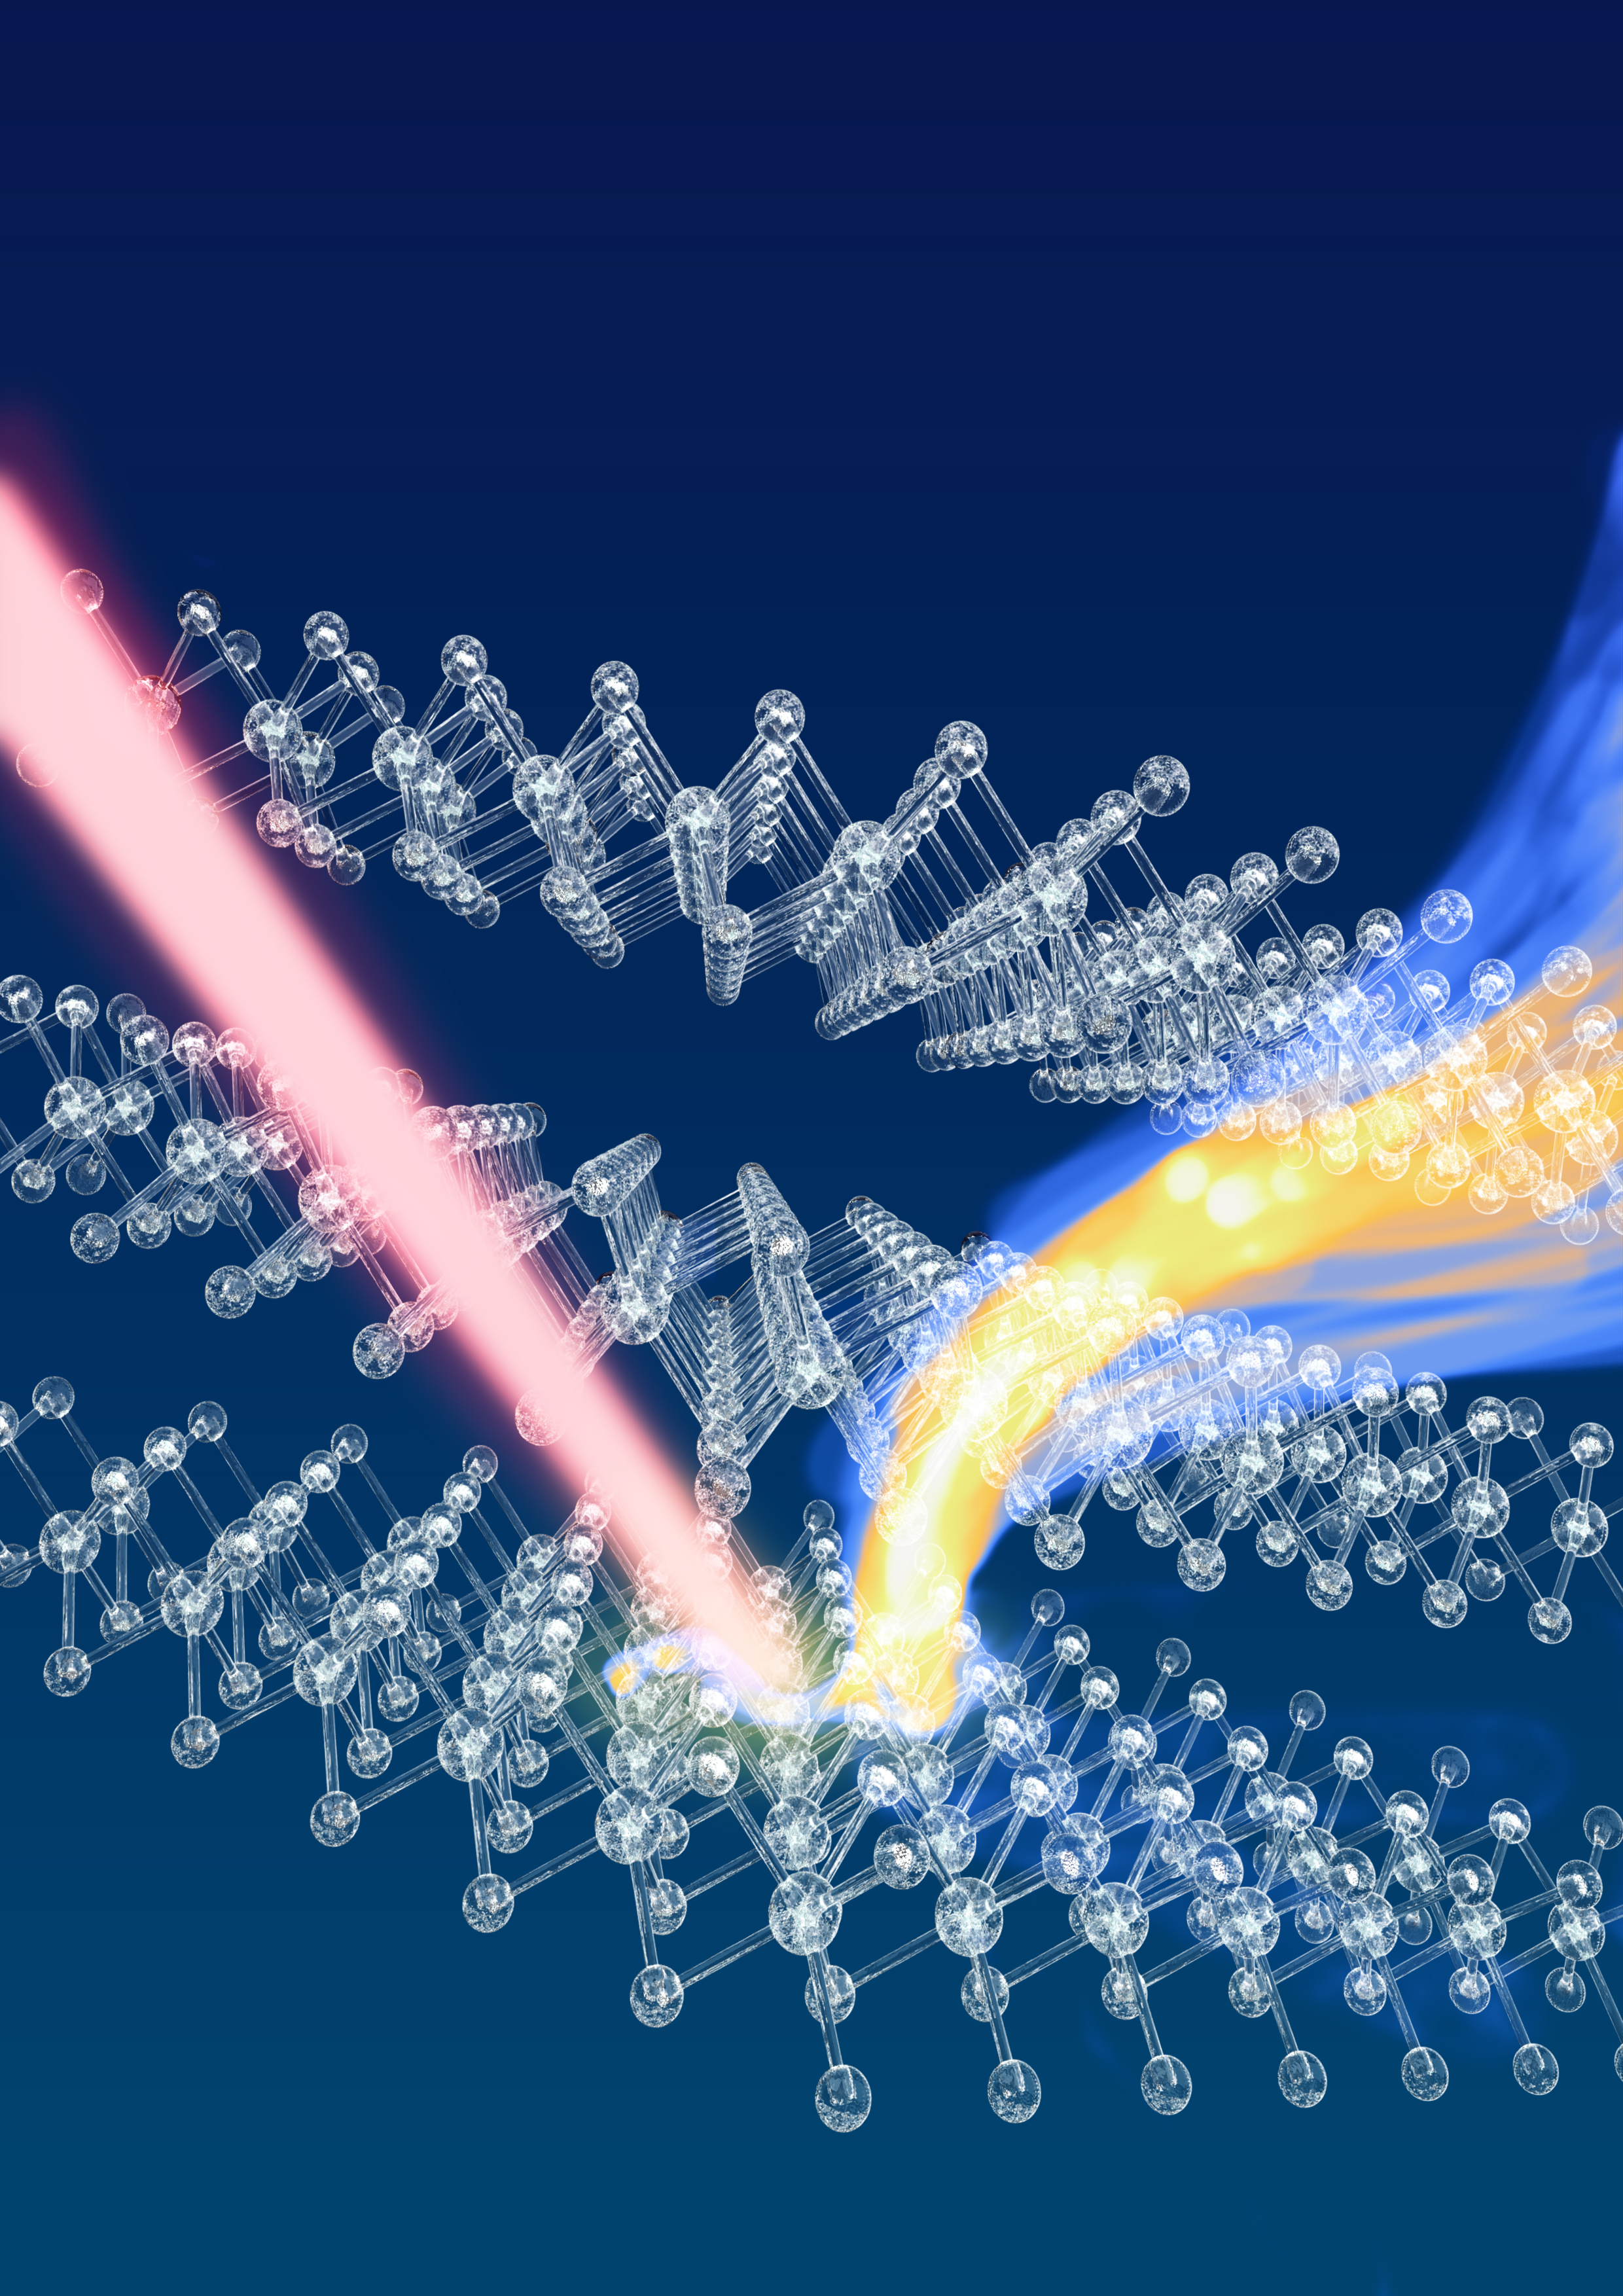
\includegraphics[width=0.6\textwidth]{Figures/Cover_v1.jpg} % 
\end{center}
\end{figure}
\end{quote}
\renewcommand{\baselinestretch}{2}
\small\normalsize

\end{center}
  %(if present, start at lower-case Roman number ii)
\addcontentsline{toc}{chapter}{Foreword}
\include{Foreword} %(if present, lower-case Roman)
\addcontentsline{toc}{chapter}{Dedication}
%Dedication

\renewcommand{\baselinestretch}{2}
\small\normalsize
\hbox{\ }
 
\vspace{.5in}

\begin{center}
\large{\textbf{\textit{Dedicated to my grandmother and my parents}}}
\end{center} 


 %(if present, lower-case Roman)
\addcontentsline{toc}{chapter}{Acknowledgements}
%Acknowledgments

\renewcommand{\baselinestretch}{2}
\small\normalsize
\hbox{\ }
 
\vspace{0in}

\begin{center}
\large{Acknowledgments} 
\end{center} 

My PhD journey in UMD is definitely one of the most memorable experience in my life. 
I would like to share my deep appreciation to all the people who helped me along the road. 
This thesis cannot be finished without contributions from them.

At first, I am deeply grateful to my advisor, Prof.You Zhou, 
for his generous support and insightful guidance throughout my PhD. 
As an advisor, he is always patient in answering my questions and provides timely feedback that helps me complete my work efficiently.

I feel truly fortunate to have worked under his supervision, where I learned not only technical skills and knowledge but, equally, integrity and a rigorous attitude toward research.



Your support shaped my approach to research and made this work possible.


\vspace{1ex}


 %(if present, lower-case Roman)
    \cleardoublepage
    \phantomsection
    \addcontentsline{toc}{chapter}{Table of Contents}
    \renewcommand{\contentsname}{Table of Contents}
\renewcommand{\baselinestretch}{1}
\small\normalsize
\tableofcontents %(required, lower-case Roman)
\newpage
\addcontentsline{toc}{chapter}{List of Tables}
    \renewcommand{\contentsname}{List of Tables}
\listoftables %(if present, lower-case Roman)
\newpage
\addcontentsline{toc}{chapter}{List of Figures}
    \renewcommand{\contentsname}{List of Figures}\listoffigures %(if present, lower-case Roman)
\newpage
% LIST OF ABBREVIATIONS
\addcontentsline{toc}{chapter}{List of Abbreviations}
%List of Abbreviations

\renewcommand{\baselinestretch}{1}
\small\normalsize
\hbox{\ }

\vspace{.5in}


\begin{center}
\large{List of Abbreviations}
\end{center} 

\vspace{3pt}

\begin{tabular}{ll}

AFM   &  Atomic Force Microscopy \\
BZ    & Brillouin zone \\
CCD   &  Charge-coupled device \\
CW   &  Continuous Wavelength \\
DBR   &  Distributed Bragg Reflector \\
EBL   & Electron-beam lithography \\
FET   &  Field-Effect Transistor \\
FWHM    & Full width at half maximum \\
hBN   &  Hexagonal Boron Nitride \\
HWP    & Half wave plate \\
ML    &  Monolayer \\
MoS$_2$  & Molybdenum disulfide \\
MoSe$_2$  & Molybdenum diselenide \\
NA   &  Numerical aperture \\
PC  &  Polycarbonate \\
PL    &  Photoluminescence \\
PFM   &  Piezoresponse Force Microscopy \\
PMMA  &  Polymethyl methacrylate \\
SEM   &  Scanning Electron Microscopy \\
TL    &  Trilayer \\
TMD   &  Transition Metal Dichalcogenide \\
TMM   &  Transfer Matrix Method \\
vdW   &   van der Waals \\
WSe$_2$ &  Tungsten Diselenide \\
1D &  One-dimensional \\
2D &  Two-dimensional \\
3D &  Three-dimensional \\

\end{tabular}

\newpage
\setlength{\parskip}{0em}
\renewcommand{\baselinestretch}{2}
\small\normalsize

%Pages from this point start at Arabic numeral 1
\setcounter{page}{1}
\pagenumbering{arabic}
%Chapter 1

\renewcommand{\thechapter}{1}

\titleformat{\chapter}[display]
  {\bfseries\Huge} % format: bold + large font
  {\chaptertitlename\ \thechapter}{20pt} % "Chapter X"
  {\Huge} % Title itself
\titlespacing*{\chapter}{0pt}{*0}{*4} % adjust spacing above/below

\chapter{Introduction}
\label{chap1}
\section{Overview}
Modern computing is under the combined pressures of scale and efficiency, and AI workloads are growing faster than improvements in transistor density and memory bandwidth\cite{Sun2015-am}.
As models get larger and memory sits farther from the processor, transferring data takes longer and consumes more energy.
Traditional copper interconnects stores charge to send a “1” and discharge to send a “0,” so a longer transfer distance require more energy every time they switch. 
They also respond more slowly because the charge has farther to go and more resistance and capacitance to overcome, which increases latency\cite{Miller2000-lm}.

Optical interconnects can transfer data by encoding electrical signal onto light with on-chip optical modulator,which can avoid Ohmic loss and enable high bandwidth over long distances\cite{Sun2015-am}.
Key building blocks for this consist electro optical modulators, high responsivity photodetectors, compact on-chip light sources(or external input coupling), low-loss waveguides/couplers, and driver electronics\cite{Miller2009-hw,Miller2010-nt}.
Among them, materials such as III–V, LiNbO$_3$, 2D semiconductors provide efficient gain, fast modulation and strong electro-optic effects\cite{Wang2018-ga,Sun2016-gg}.
Among these building blocks, the electro–optic modulator (EOM) is especially critical, as it sets the link bandwidth and energy per bit and largely determines extinction ratio and noise.
The modulation efficiency arises from the material’s nonlinear optical response as function of the electrical field or doping density. 
The induced changes in absorption and refractive index then can convert small electrical drives into large optical contrast. 
In the classical regime, large modulation depth typically requires many photons or high optical fields\cite{Miller2009-hw}. 

2D semiconductors provide strong excitonic behavior which can be easily tuned by the gating voltage. 
This enable the application in ultra compact and low voltage modulator.

Optical computing leverages photons to perform signal processing and computation with intrinsically high bandwidth, low latency, and reduced energy dissipation\cite{Miller2010-nt}. 
Because photons are massless and do not experience resistive losses, optical links can achieve lower energy per bit and avoid the RC bottlenecks that limit charge-based electronics. 

Despite these advantages, a major challenge for all-optical logic is the weakness of optical nonlinearities in conventional materials\cite{Boyd2020-re}. 
Since photons do not interact in linear media, and inducing a significant optical response typically requires high field intensities or large photon numbers\cite{Chang2014-hk}. 
Current optical switches based on the Kerr effect or free carrier modulation require elevated power levels for fast modulation, leading to effects such as two-photon absorption, excess carrier and heat generation\cite{Miller2009-hw}.
These side effects inject noise and cause thermal drift, especially when many devices are integrated on the same chip.

A promising path forward is to enter the quantum nonlinear regime, where even a few photons can interact strongly. 
One key goal is to achieve photon blockade, in which the presence of a single photon shifts the system energy to prevent the entry of a second\cite{Imamoglu1997-pb}. 
This enables single photon switches, quantum logic gates, and generation of nonclassical light source, all essential components for scalable quantum photonic circuits\cite{Lodahl2015-el,Chang2014-hk}. 
However, realizing photon blockade requires nonlinear energy shifts that exceed the linewidth\cite{Carusotto2013-mf}. 

Photon blockade requires anharmonic shift $U \geq \Gamma$, where $\Gamma=\kappa+\gamma^\ast$ is the total linewidth including cavity decay $\kappa$ and pure dephasing $\gamma^\ast$~ \cite{Birnbaum2005-ix,Verger2006-jz}. 
For a Kerr medium, the $U$ is proportional to $g /A_{\mathrm{eff}}$, where $g$ is a property from the material nonlinear coupling. $A_{\mathrm{eff}}$ the optical mode area. 
In standard dielectric or III–V cavities, one typically finds $g \sim 0.1$–$1~\mu\mathrm{eV}\cdot\mu\mathrm{m}^2$ and $A_{\mathrm{eff}}\sim 5$–$20~\mu\mathrm{m}^2$.
This gives out an overall $U\sim 0.01$–$0.2~\mathrm{meV}$, which is usually below $\Gamma\sim 0.2$–$2~\mathrm{meV}$ even at cryogenic temperatures. 
That's why it's challenging in realizing this in conventional materials or systems.

2D semiconductors offer a unique opportunity to bridge this gap. 
Their tightly bound excitons exhibit large oscillator strengths and support strong exciton exciton interactions, giving rise to large Kerr-like optical nonlinearities\cite{Wang2018-qm}. 
These interactions can be further enhanced by coupling to optical cavities\cite{Datta2022-po,Walther2018-jp}, engineering moiré potentials\cite{Zhang2021-eb}, or applying spatial confinement\cite{Thureja2022-yc}, pushing device operation into the few-photon regime. 
The atomically thin nature of 2D materials enables ultra compact devices and high density integration via van der Waals stacking, compatible with silicon photonics and CMOS platforms\cite{de-Abajo2025-vm}. 
Moreover, gate tunable carrier densities and valley control offer additional knobs to optimize modulation speed, contrast, and noise\cite{Mak2012-le}. 
The intrinsically short radiative lifetime of excitons\cite{Wang2018-zb}, while challenging for photon statistics measurements, are advantageous for creating single-photon sources with high repetition rates and ultrafast optical switches\cite{Korzh2020-ya,Esmaeil-Zadeh2020-mp}. 

In summary, no matter for classical and quantum nonlinear optics applications, enhancing the interaction strength among optical excitations and reducing their linewidth are critical goals.
While challenges remain in materials growth, theoretical understanding and device engineering, the outlook for 2D materials in nonlinear optics is overwhelmingly positive. 
Their properties coupled with ongoing innovations, position them as transformative building blocks for the next generation of optical technologies. 

\section{Thesis Outline}
This thesis focus on developing systems with large exciton interactions towards giant optical nonlinearity.
Chapter~\ref{chap2} will discuss the background of excitons, exciton-polaritons and the related physics about TMD semiconductors. 
Chapter~\ref{chap3} will introduce the experimental and numerical methods applied through the thesis.
Chapter~\ref{chap4} will discuss the approach towards exciton quantum confinement with novel electrostatic superlattice.
Chapter~\ref{chap5} will introduce the developed system with giant optical nonlinearity of Fermi polarons, where the exciton-carrier interaction contributes to this large nonlinear shift.
Chapter~\ref{chap6} will discuss the ongoing project based on Chap.~\ref{chap5} that we leverage cavity engineering for realizing polaron-polariton with enhanced optical nonlinearity.
Chapter~\ref{chap7} summarize the whole thesis and discuss the future directions of the work.



%Chapter 2

\renewcommand{\thechapter}{2}

\chapter{Background of the system}

\section{Basic structure of 2D Transition Metal Dichalcogenides}

\subsection{Lattice Structure}
Transition metal dichalcogenides(TMD) semicondcutor have the general chemical formula of $MX_2$, where $M$ refers to the transition metal atom($Mo,W$) and $X$ is the chalcogen atom($S$,$Se$,$Te$).
In the TMD bulk crystal, the metal and chalcogen atoms are bonded through covalent-ionic bonds, whereas different layers are bonded by the weak van der Waals force.
This enables accessing the monolayer TMD through mechanical exfoliation.
There are three different phases in the TMD crystal: hexagonal 2H, rhombohedral 3R, and trigonal 1T' phases. In their most thermaldynamic stable phase 2H polytype, a monolayer consists of a hexagonal plane of transition metal atoms sandwiched between two planes of chalcogen atoms, forming trigonal prismatic coordination.
This yields a honeycomb-like lattice with \textbf{$D_{3h}$} 
point-group symmetry at the monolayer level, with the absence of inversion symmetry. 
However, this inversion symmetry can be restored in even number multilayers, with one layer is rotated $180^\circ$ relative to the other layer.

In 3R phase, each successive monolayer is shifted relative to the one below, following an ABC stacking order and belongs to the \textbf{$C_{3v}$}point group rather than the AB sequence of the 2H phase. 
This stacking is characterized by the absence of inversion symmetry at all thicknesses. 
As a result, strong second-order nonlinear optical processes, such as second-harmonic generation, have been extensively investigated in 3R multilayers\cite{Xu2022-at,Qin2024-xt}.

The 1T phase, by comparison, features octahedral coordination of the transition-metal atoms with $D_{3d}$ point-group symmetry, which includes inversion symmetry even at the monolayer level.
While the ideal 1T structure is metallic, certain compounds undergo lattice distortions into the so-called 1T$^{\prime}$ phase, which breaks inversion symmetry and can host semimetallic or topologically nontrivial states, including quantum spin Hall insulators and type-II Weyl semimetals.
%%figure1-1
\renewcommand{\baselinestretch}{2}
\small\normalsize
\begin{quote}
\begin{figure}
\begin{center}
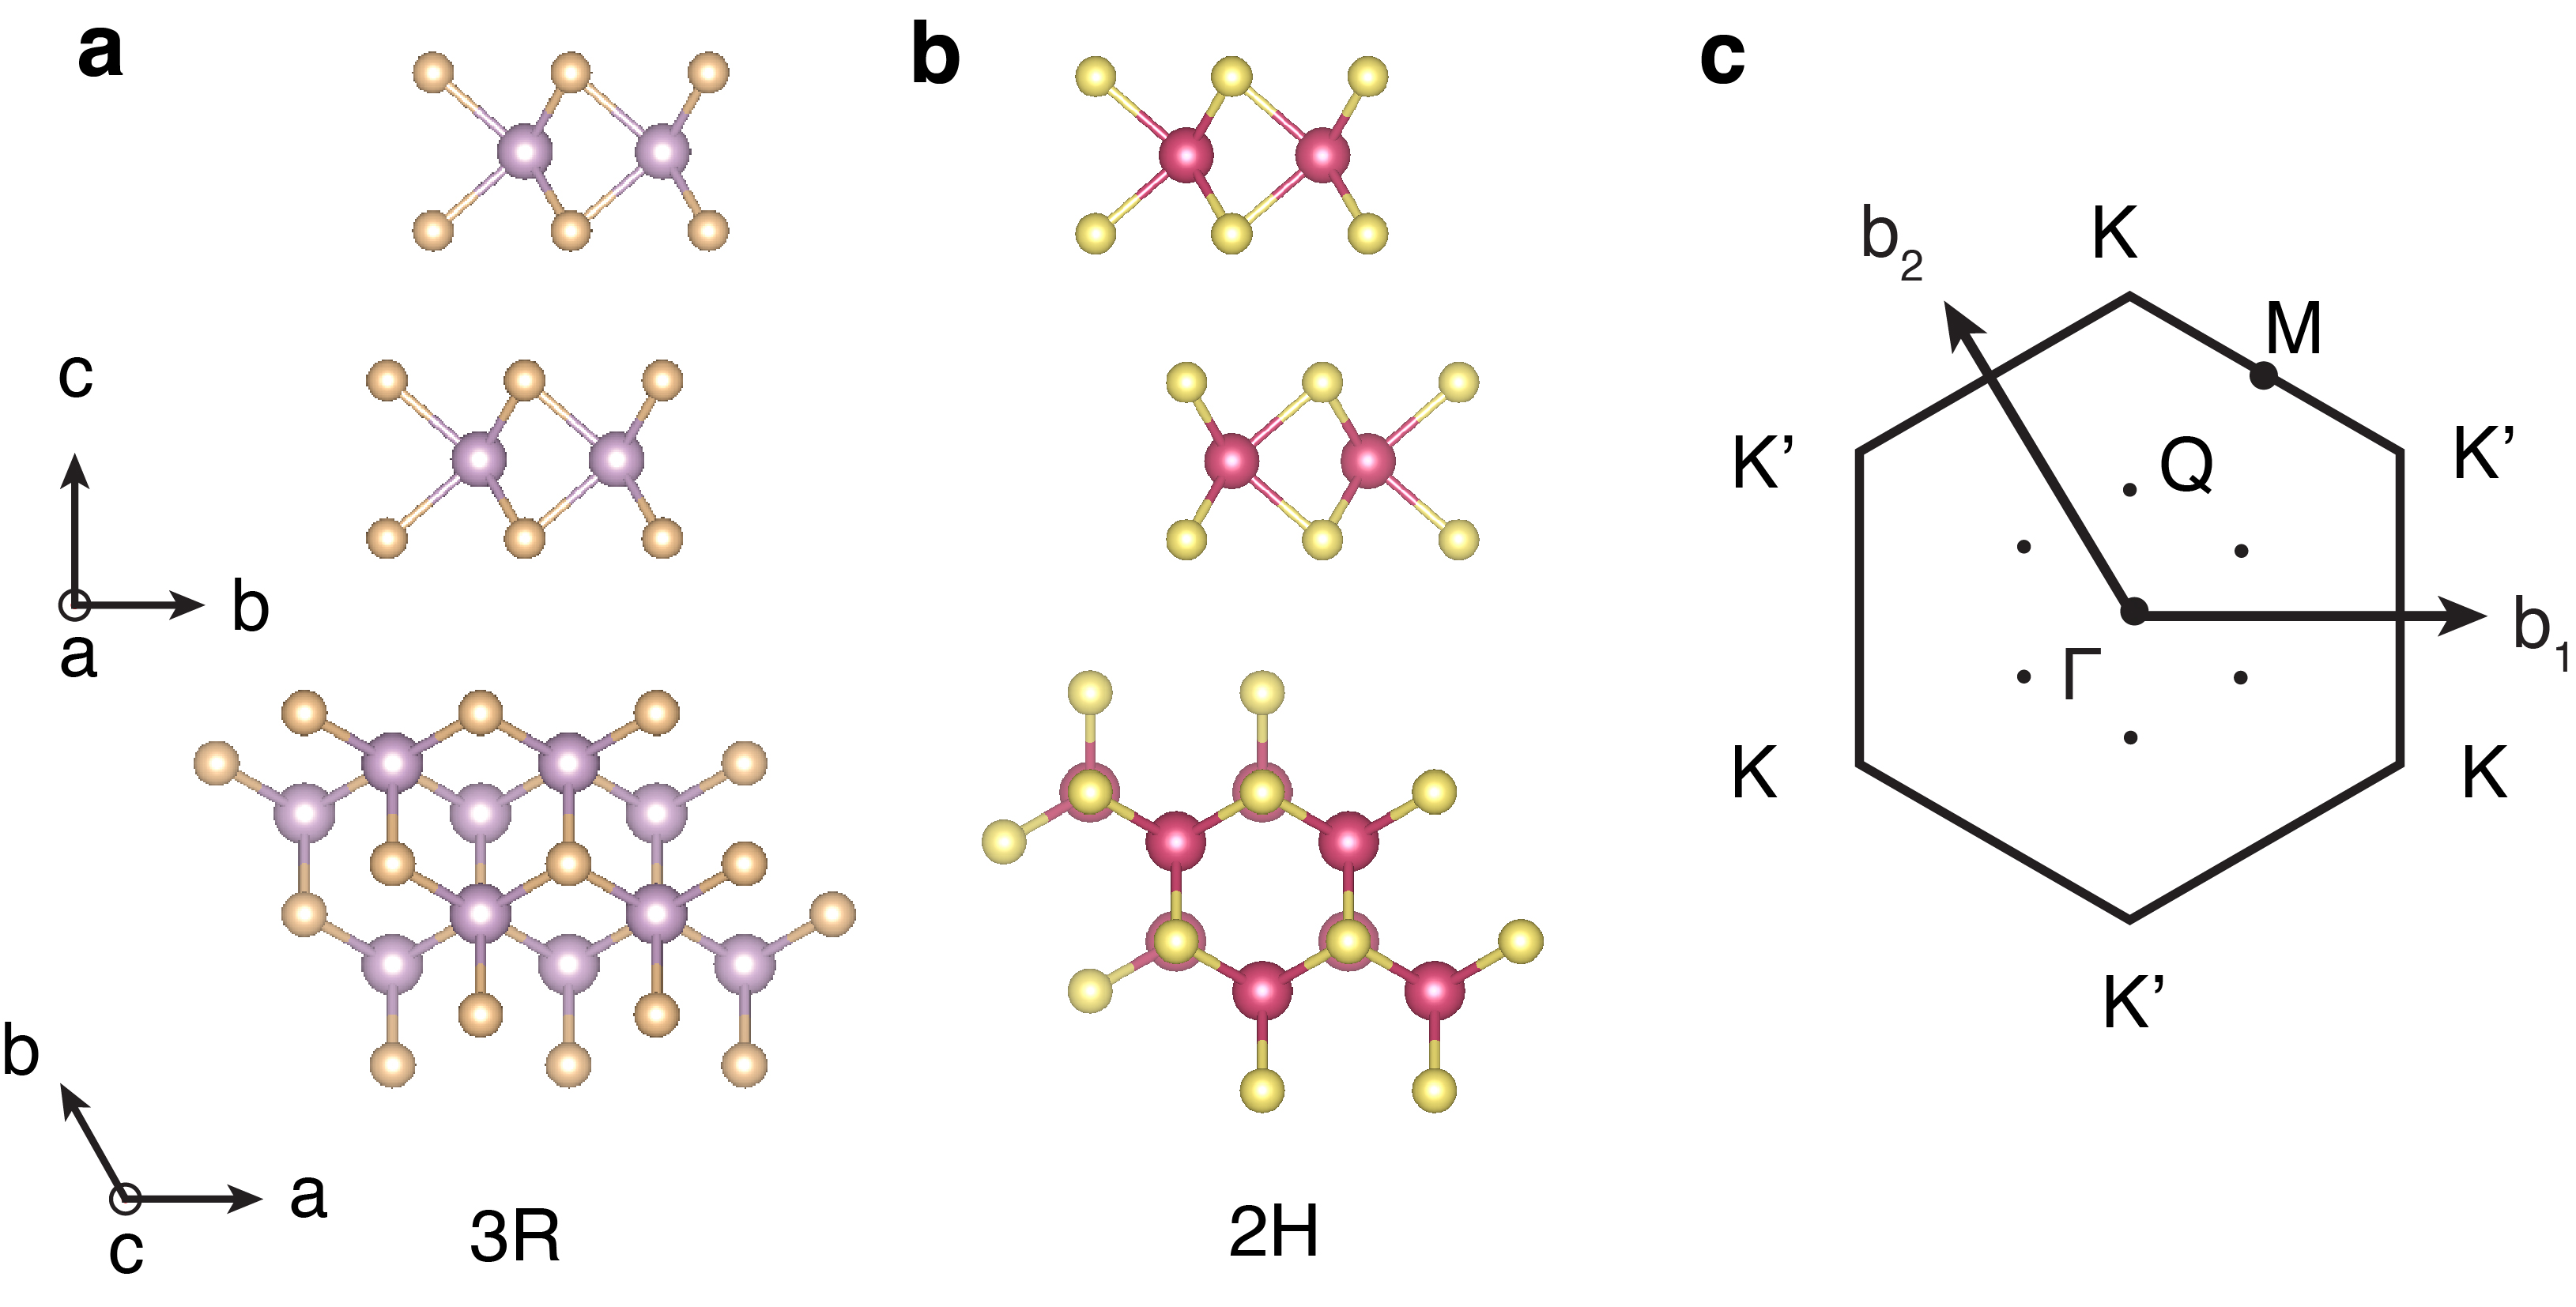
\includegraphics[width=0.85\textwidth]{Figures/C2/Fig.2-1_lattice.jpg}%
\end{center}
\caption[\textbf{Crystal structures of TMDC.}]{\textbf{a,b,} Side view (top) and top view (bottom) of the 3R and 2H stacking structure. 
\textbf{c,} Hexagonal Brillouin zone of TMD with the reciprocal lattice vectors $\mathbf{b_1}$ and $\mathbf{b_2}$.}
\label{fig.lattice}
\end{figure}
\end{quote}
\renewcommand{\baselinestretch}{2}
\small\normalsize
% ------

\subsection{Electronic band structure of TMD}
In this thesis, we mainly study the layers mechanically exfoliated from 2H phase TMD. The discussion of the electronic bandstructure would thus mainly focus on the 2H phase. 

For the semicondcutor TMDCs, the bandgap is around 1 to 2 eV\cite{Manzeli2017-nt}.
In the monolayer TMD, the conduction band minimum and valence band maximum located at the corner of the Brillouin zone $K$ ($K^\prime$) valley, which is mainly derived from the transition-metal $d$ orbitals ($d_{z^2}$ for the conduction band and $d_{x^2-y^2}$ + $d_{xy}$ for the valence band)\cite{Liu2013-jh}. 
%%figure1-2
\renewcommand{\baselinestretch}{2}
\small\normalsize
\begin{quote}
\begin{figure}
\begin{center}
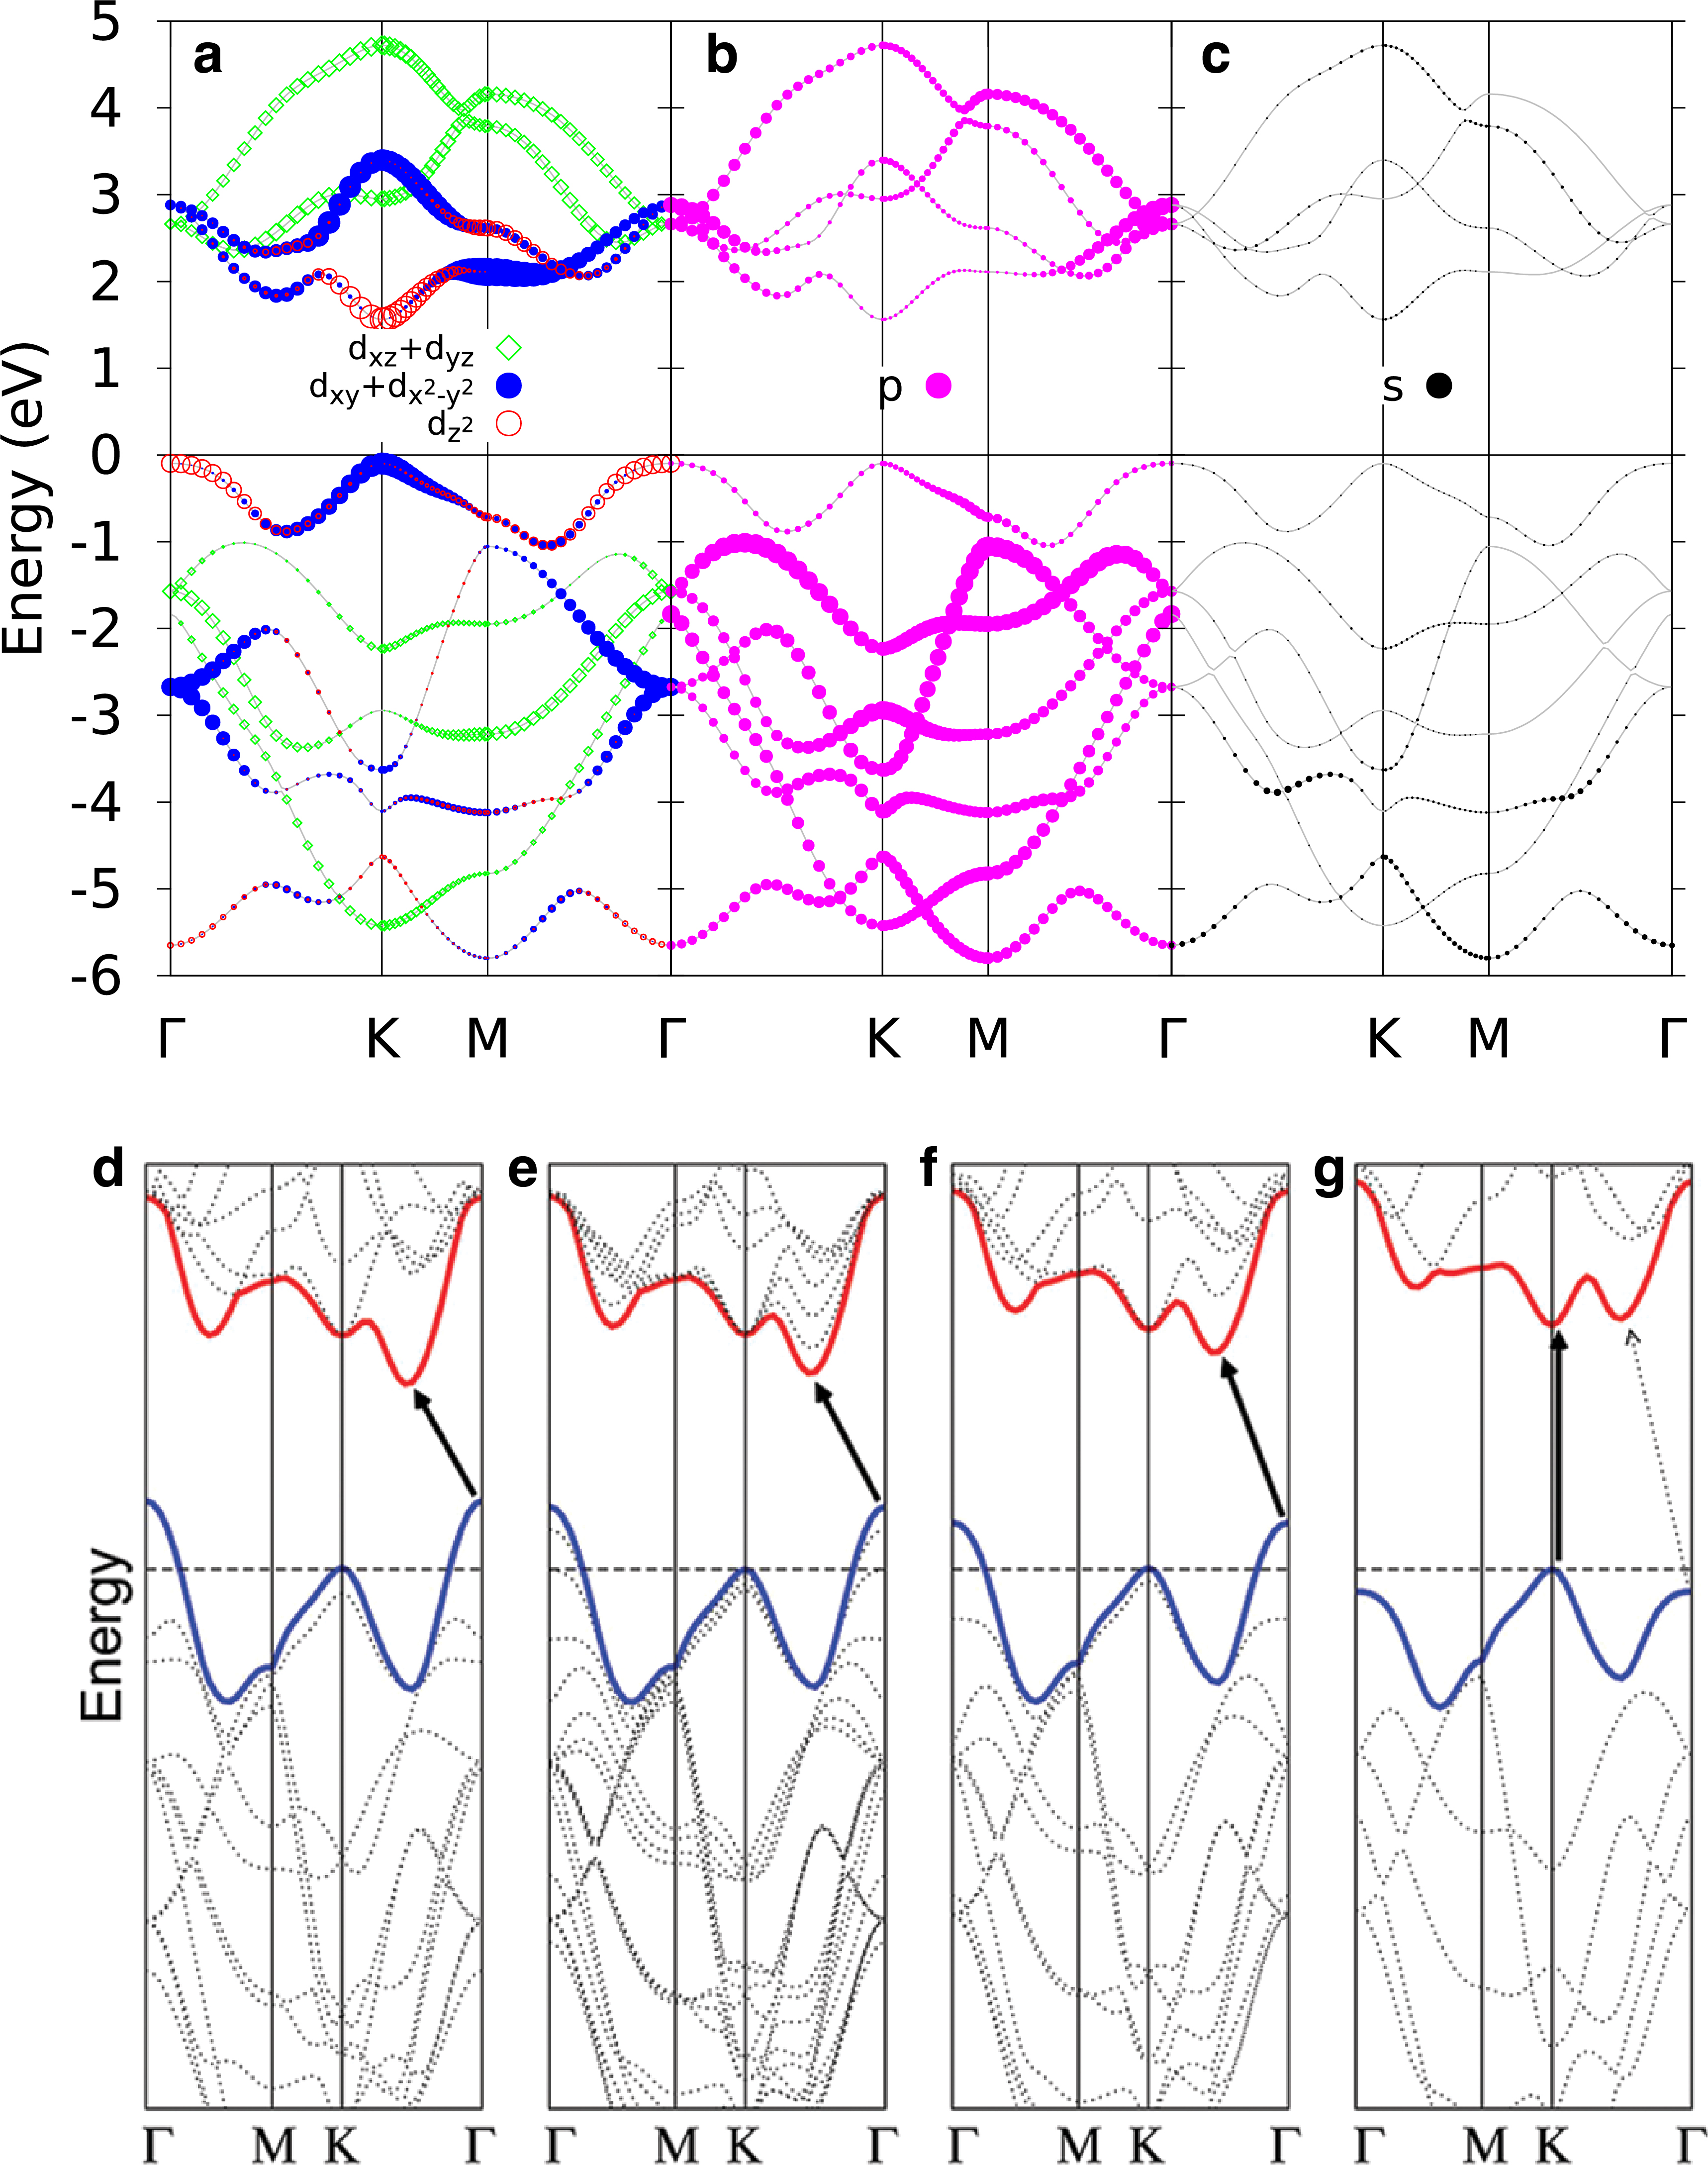
\includegraphics[width=0.65\textwidth]{Figures/C2/Fig.2-2_bandstructure.jpg}%
\end{center}
\caption[\textbf{Band structures of TMDC.}]{\textbf{a,b,c} Calculated orbital projected band structure for monolayer $MoS_2$, with \textbf{a} contribution from the Mo atom $d$ orbitals;\textbf{b}Total $p$ orbitals dominated by the chalcogen S atom; \textbf{c} Total $s$ orbital.
\textbf{d,e,f,g} Calculated bandstructure of bulk,quadrilayer,bilayer and monolayer TMD(from left to right).
The crossover from indirect to direct bandstructure happens at the monolayer limit.Figure adpated from\cite{Splendiani2010-km,Liu2013-jh}.}
\label{fig.band}
\end{figure}
\end{quote}
\renewcommand{\baselinestretch}{2}
\small\normalsize

One well-known feature of the TMD materials is the indirect to direct band structure transition when the layer thickness is approaching to the monolayer limit\cite{Mak2010-dq}.
This crossover arises from the different sensitivity of electronic states at distinct wave vectors to interlayer coupling and quantum confinement\cite{Splendiani2010-km}.
At the k points, states are strongly localized around the metal atoms and therefore remain largely unaffected by interlayer coupling. 
In contrast, the valence states near $\Gamma$ and the conduction states near the $Q$ valley (between $\Gamma$ and $K$) originate from hybridization between transition-metal $d$ orbitals 
and chalcogen $p_z$ orbitals. 
Because the $p_z$ orbitals extend out of plane, they are more 
delocalized and thus highly sensitive to interlayer coupling. 
As a result,with increasing layer numbers lifts the $\Gamma$ valence band upward and lowers the $Q$ conduction band, while the $K$ valleys remain nearly unchanged.
Figure~\ref{fig.band} shows this direct–indirect crossover in the calculated bandstructures.

\subsection{Spin-orbit interaction}
Spin--orbit coupling (SOC) arises from the relativistic interaction between an electron’s orbital motion and its spin. 
In the effective one-electron picture, the SOC Hamiltonian can be expressed as
\begin{equation}
H_{\mathrm{SOC}} = \xi(r)\, \mathbf{L}\cdot\mathbf{S}
\label{eq.SOC}
\end{equation}
where $\mathbf{L}$ and $\mathbf{S}$ are the orbital and spin angular momenta, and $\xi(r)$ denotes the radial SOC strength, which increases strongly with atomic number\cite{Sakurai2020-jh,Winkler2003-ty}. 
In transition-metal dichalcogenides (TMDs), the heavy transition-metal atoms (Mo, W) provide a strong SOC environment that directly impacts the band edges\cite{Xiao2012-pw,Liu2013-jh}.
At the $K$ and $K'$ valleys, the valence-band maximum is primarily derived from in-plane $d_{x^2-y^2}$ and $d_{xy}$ orbitals. 
In the complex orbital basis, these states correspond to magnetic quantum numbers $m_l = \pm 2$, which carry significant angular momentum around the $z$-axis. 
Their strong coupling to spin through the $L_z S_z$ interaction results in a large spin splitting, typically several hundred meV, especially for W-based TMD\cite{Kormanyos2015-dn,Zhu-Z-Y-and-Cheng-Y-C-and-Schwingenschl-ogl-U2011-lo}.
In contrast, the conduction-band minimum originates mainly from the $d_{z^2}$ orbital ($m_l = 0$), which carries zero orbital angular momentum projection along $z$. 
However, the calculation of the bandstructure shows a finite spin splitting in the value of a few meV in the conduction band.
This arises through SOC-mediated coupling of the 
$d_{z^2}$ state to nearby orbitals that carry finite angular momentum ($m_l = \pm 1$), most importantly the transition-metal $d_{xz}/d_{yz}$ and chalcogen $p_x/p_y$ states\cite{Liu2013-jh,Kosmider2013-bt}. 
In MoX$_2$, this interaction produces a negative splitting, so the lower conduction subband has the opposite spin orientation to the valence-band maximum. 
In contrast, WX$_2$ compounds exhibit a positive splitting, and the conduction subband ordering is reversed\cite{Liu2013-jh}.
The broken inversion symmetry together with strong spin–orbit coupling in monolayer TMDs gives rise to spin–valley coupling, which enables control of valley degrees of freedom through phenomena such as the valley Hall effect and valley-selective optical transitions\cite{Mak2012-le,Cao2012-tt,Xiao2012-pw}.

\subsection{Valley-Dependent Optical Selection Rules}
Optical transitions in semiconductors are governed by the electric-dipole selection rule, 
which enforces conservation of angular momentum between the electron system and the absorbed or emitted photon\cite{Yu2010-yp,Fox2010-ly}. 
The corresponding transition amplitude can be written as\cite{Fox2010-ly}:
\begin{equation}
M_{\pm}(\mathbf{k}) = \big\langle \psi_{c}(\mathbf{k}) \big| 
\hat{\mathbf{p}} \cdot \mathbf{e}_{\pm} 
\big| \psi_{v}(\mathbf{k}) \big\rangle,
\label{eq.OP transition}
\end{equation}
where $\psi_{v}$ and $\psi_{c}$ denote the valence- and conduction-band Bloch states,
$\hat{\mathbf{p}}$ is the momentum operator, and
$\mathbf{e}_{\pm} =\frac{1}{\sqrt{2}} (\hat{x} \pm i\hat{y})$ are polarization vectors for right- ($\sigma^{+}$) and left- ($\sigma^{-}$) handed circularly polarized light\cite{Teich1991-lv}.
Because $\mathbf{e}_{\pm}$ carries angular momentum projection $\pm \hbar$ along the light propagation axis, a circularly polarized photon transfers angular momentum $\pm 1$ into the electronic system\cite{Fox2010-ly}. 
Thus, optical excitation with $\sigma^+$ or $\sigma^-$ light can
be used to probe states that differ in their orbital angular momentum by one unit\cite{Cao2012-tt,Xiao2012-pw,Mak2012-le}.

In semiconducting TMD monolayers, the broken inversion symmetry and strong spin--orbit coupling translate these general rules into valley-specific selection rules\cite{Xiao2012-pw}. 
The valence band maximum at the inequivalent $K$ and $K'$ valleys is dominated by metal $d_{x^2-y^2}$ and $d_{xy}$ orbitals, which combine as $d_{x^2-y^2} \pm i d_{xy}$ and carry angular momentum projections $m_l = \pm 2$.
The conduction band minimum is mainly derived from the $d_{z^2}$ orbital ($m_l=0$)\cite{Liu2013-jh}. 
Interband optical transitions are therefore allowed only if the angular momentum of the photon compensates the orbital character of the valence state. 
As a consequence, transitions at the $K$ valley couple exclusively to $\sigma^+$ photons, while those at $K'$ couple only to $\sigma^-$ photons as shown in Figure~\ref{fig.selection-rule}.

%Fig.5--------------
\renewcommand{\baselinestretch}{1}
\small\normalsize
\begin{quote}
\begin{figure}
\begin{center}
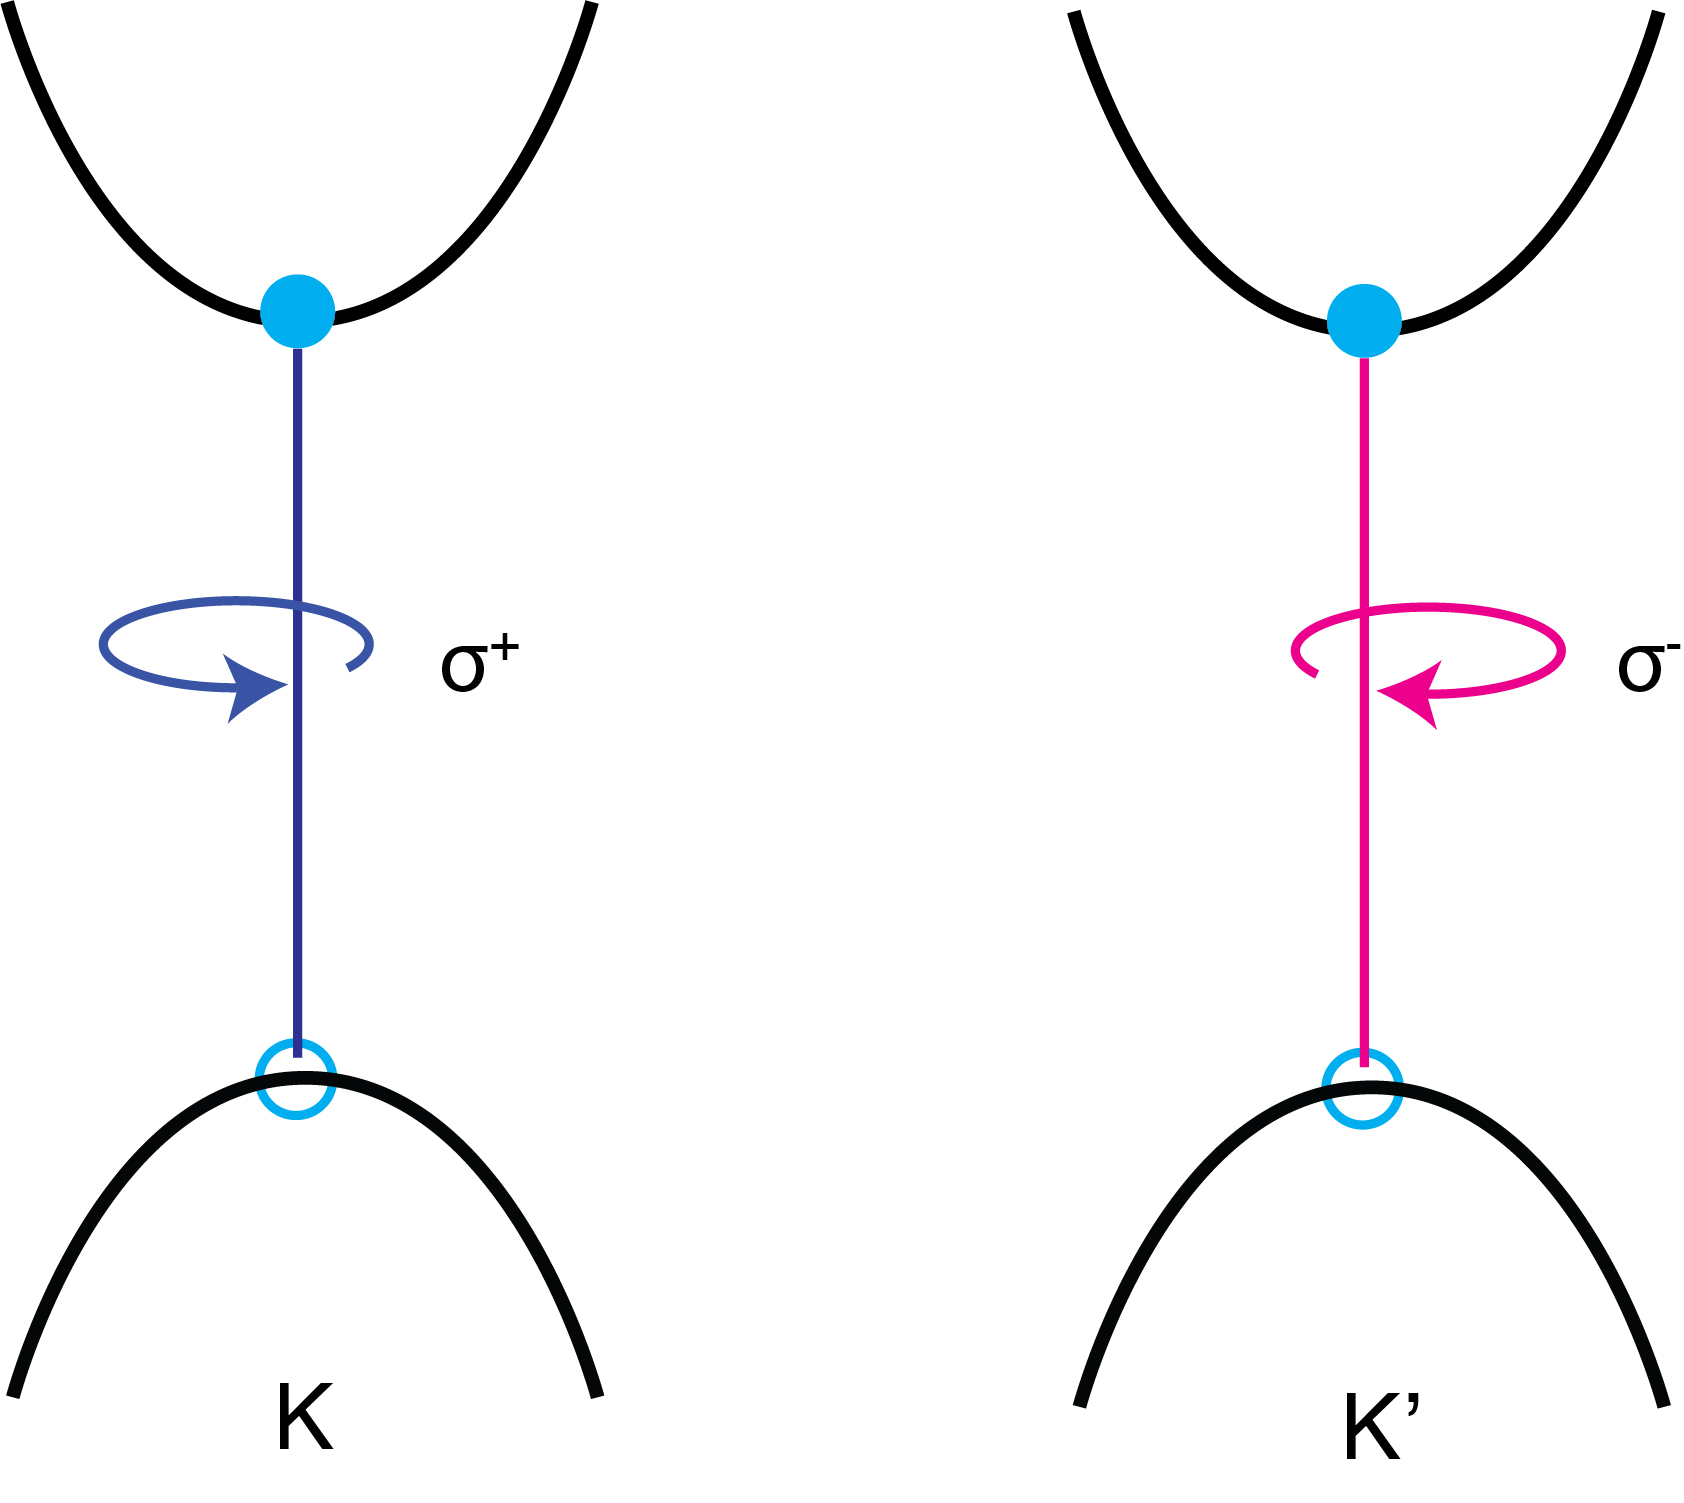
\includegraphics[width=0.4\textwidth]{Figures/C2/Fig.selection_rule.jpg} % 
\end{center}
\caption[Valley-dependent optical selection rule] {\textbf{Valley-dependent optical selection rule.}The left and right circular polarized light coupled to the $K$ and $K^\prime$ valley, respectively.}
\label{fig.selection-rule}
\end{figure}
\end{quote}
\renewcommand{\baselinestretch}{2}
\small\normalsize
% --------------
This valley--helicity locking gives rise to valley-selective circular dichroism, as demonstrated in monolayer MoS$_2$ \cite{Mak2012-le,Zeng2012-ss}. 
The experimental observation of nearly perfect polarization selectivity provides direct evidence that inversion symmetry
breaking is essential for lifting valley degeneracy in optical transitions.

However, in bilayer TMDs with 2H stacking, where the top layer is rotated by $180^{\circ}$ relative to the bottom layer, the inversion
symmetry is restored, and the valley-dependent optical selection rules are lost: both valleys can now couple to both helicities with equal weight. 
As a result, bilayer MoS$_2$ shows no net circular dichroism under optical excitation \cite{Mak2012-le}. 
This striking contrast between monolayer and bilayer systems highlights the crucial role of symmetry:
broken inversion symmetry in monolayers enforces a one-to-one correspondence between photon helicity and valley index, while the restoration of inversion symmetry in bilayers removes this correspondence and suppresses valley polarization.

In summary, the valley-contrasting optical selection rules in monolayer TMDs originate from the unique orbital composition of the band edges and the absence of inversion symmetry. 
These rules form the microscopic basis of valley-selective optical excitation and detection, establishing light helicity as a powerful handle to manipulate valley degrees of freedom in two-dimensional semiconductors\cite{Yu2017-jb}.

\section{Excitons in TMDs}
When the semiconductor absorbs a photon with energy greater than its band gap, an electron would be promoted from the valence band to the conduction band and leaves a positively charged hole in the valence band. 
The Coulomb attraction between the negatively charged electron and the hole can lead to the formation of a bound electorn-hole pair called exciton\cite{Fox2010-ly,Yu2010-ae}. 

Excitons can be classified into two types depending on the spatial extent of the electron--hole wavefunction. 
Frenkel excitons, typically exist in molecular crystals and insulators, are tightly bound and localized on the scale of one unit cell. 
In contrast, Wannier–Mott excitons have a larger radius and extend over many unit cells, so their center of mass can propagate through the crystal. 
Owing to this spatial delocalization, they are commonly referred to as free excitons.

\subsection{Wannier equation and binding energy}
The energy of the exciton can be obtained by solving the two-body Schrödinger equation, which can be written in relative and center-of-mass coordinates. 
The relative motion based on the effective mass can be described by the Wannier equation\cite{Yu2010-ae}:
\begin{equation}
-\left[ \frac{\hbar^2}{2\mu} \nabla^2 + V(\textbf{r}) \right] \psi_{n}(\textbf{r}) 
= E_{n} \, \psi_{n}(\textbf{r})
\label{eq:wannier}
\end{equation}
where $\mu =\frac {m_e m_h}{(m_e+m_h)}$ is the reduced mass,$\psi_{n}(r)$ is the exciton wavefunction. $V(r)$ is the Coulomb interaction, and $E_n$ are the excitonic eigenenergies below the band gap $E_g$. 
$V(r)$ has the Coulomb form as:
\begin{equation}
V(\textbf{r}) = - \frac{e^2}{4\pi \varepsilon_0 \varepsilon_r \textbf{r}}
\label{eq:coulomb}
\end{equation}
By solving the Wannier equation with 3D and 2D Laplace operator in polar coordinates, we can obtain the exciton binding energies follow a Rydberg series\cite{Chernikov2014-vo,Yu2010-ae}:
\begin{flalign}
E_{B,3D}^{(n)} = - \frac{R_X}{n^2} \quad n = 1,2,3,\dots \\[6pt]
E_{B,2D}^{(n)} = - \frac{R_X}{(n-\frac{1}{2})^2},\quad n = 1,2,3,\dots 
\label{eq:exciton_rydberg}
\end{flalign}
$n$ is the principal quantum number, $E_{B,3D}^{(n)}$ is the exciton binding energy in three dimension and $E_{B,2D}^{(n)}$ is the binding energy in 2D plane.$R_X$ is the exciton Rydberg energy and can be expressed as 
$R_X = \frac{\mu}{m_0\varepsilon_r^2}R_H$. $R_H$ is the Rydberg energy of the hydrogen atom(13.6 eV). $\mu$ refers to the reduced electron--hole mass and $\varepsilon_r$ is the relative dielectric
constant. 
The exciton binding energy and the electronic band gap would have the relationship shown as:
\begin{equation}
E_n = E_g-E_{B,2D/3D}^{(n)}
\label{eq:optical gap}
\end{equation}\vspace{-0.5em}
where $E_g$ is the quasiparticle band gap, $E_n$ is the optical band gap when $n =1$. The corresponding exciton Bohr radius for the 1S exciton in 3D and 2D can be obtained as:
\begin{align}
a_{B,3D} &= \frac{4\pi \varepsilon_0 \varepsilon_r \hbar^2}{\mu e^2} 
           = a_0 \cdot \frac{\varepsilon_r}{\mu/m_0} \\[6pt]
a_{B,2D} &= \frac{2\pi \varepsilon_0 \varepsilon_r \hbar^2}{\mu e^2} 
           = a_0 \cdot \frac{\varepsilon_r}{2\mu/m_0} 
           = \frac{1}{2} a_{B,3D}
\label{eq:exciton_bohr_radius}
\end{align}
The $a_0$ value refers to the atomic Bohr radius. 
Compared to the 3D case, the 1s exciton confined to a 2D plane exhibits a binding energy that is enhanced by a factor of four.
This can be understood that when the dimensionality is reduced from 3D to 2D, the exciton cannot spread out in all three spatial directions.
Instead, the electron and hole are forced to remain in the same plane, which increases their spatial overlap. 
This increased overlap enhance the Coulomb attraction, leading to a smaller Bohr radius and larger binding energy in the 2D plane.
In real experiments, TMDs are typically studied in device structures encapsulated by dielectric hBN to prevent any inhomogeneous perturbation,and it has a relatively low permittivity of about 3\cite{Hunt2013-ma}.
This weak screening further enhances the Coulomb interaction, resulting in a much larger exciton binding energy($\sim$ 500 meV)\cite{Wang2018-my} compared to that in GaAs quantum wells($\sim$ tens of meV)\cite{Nakwaski1995-hc}.

%Fig.1-4--------------
\renewcommand{\baselinestretch}{1}
\small\normalsize
\begin{quote}
\begin{figure}
\begin{center}
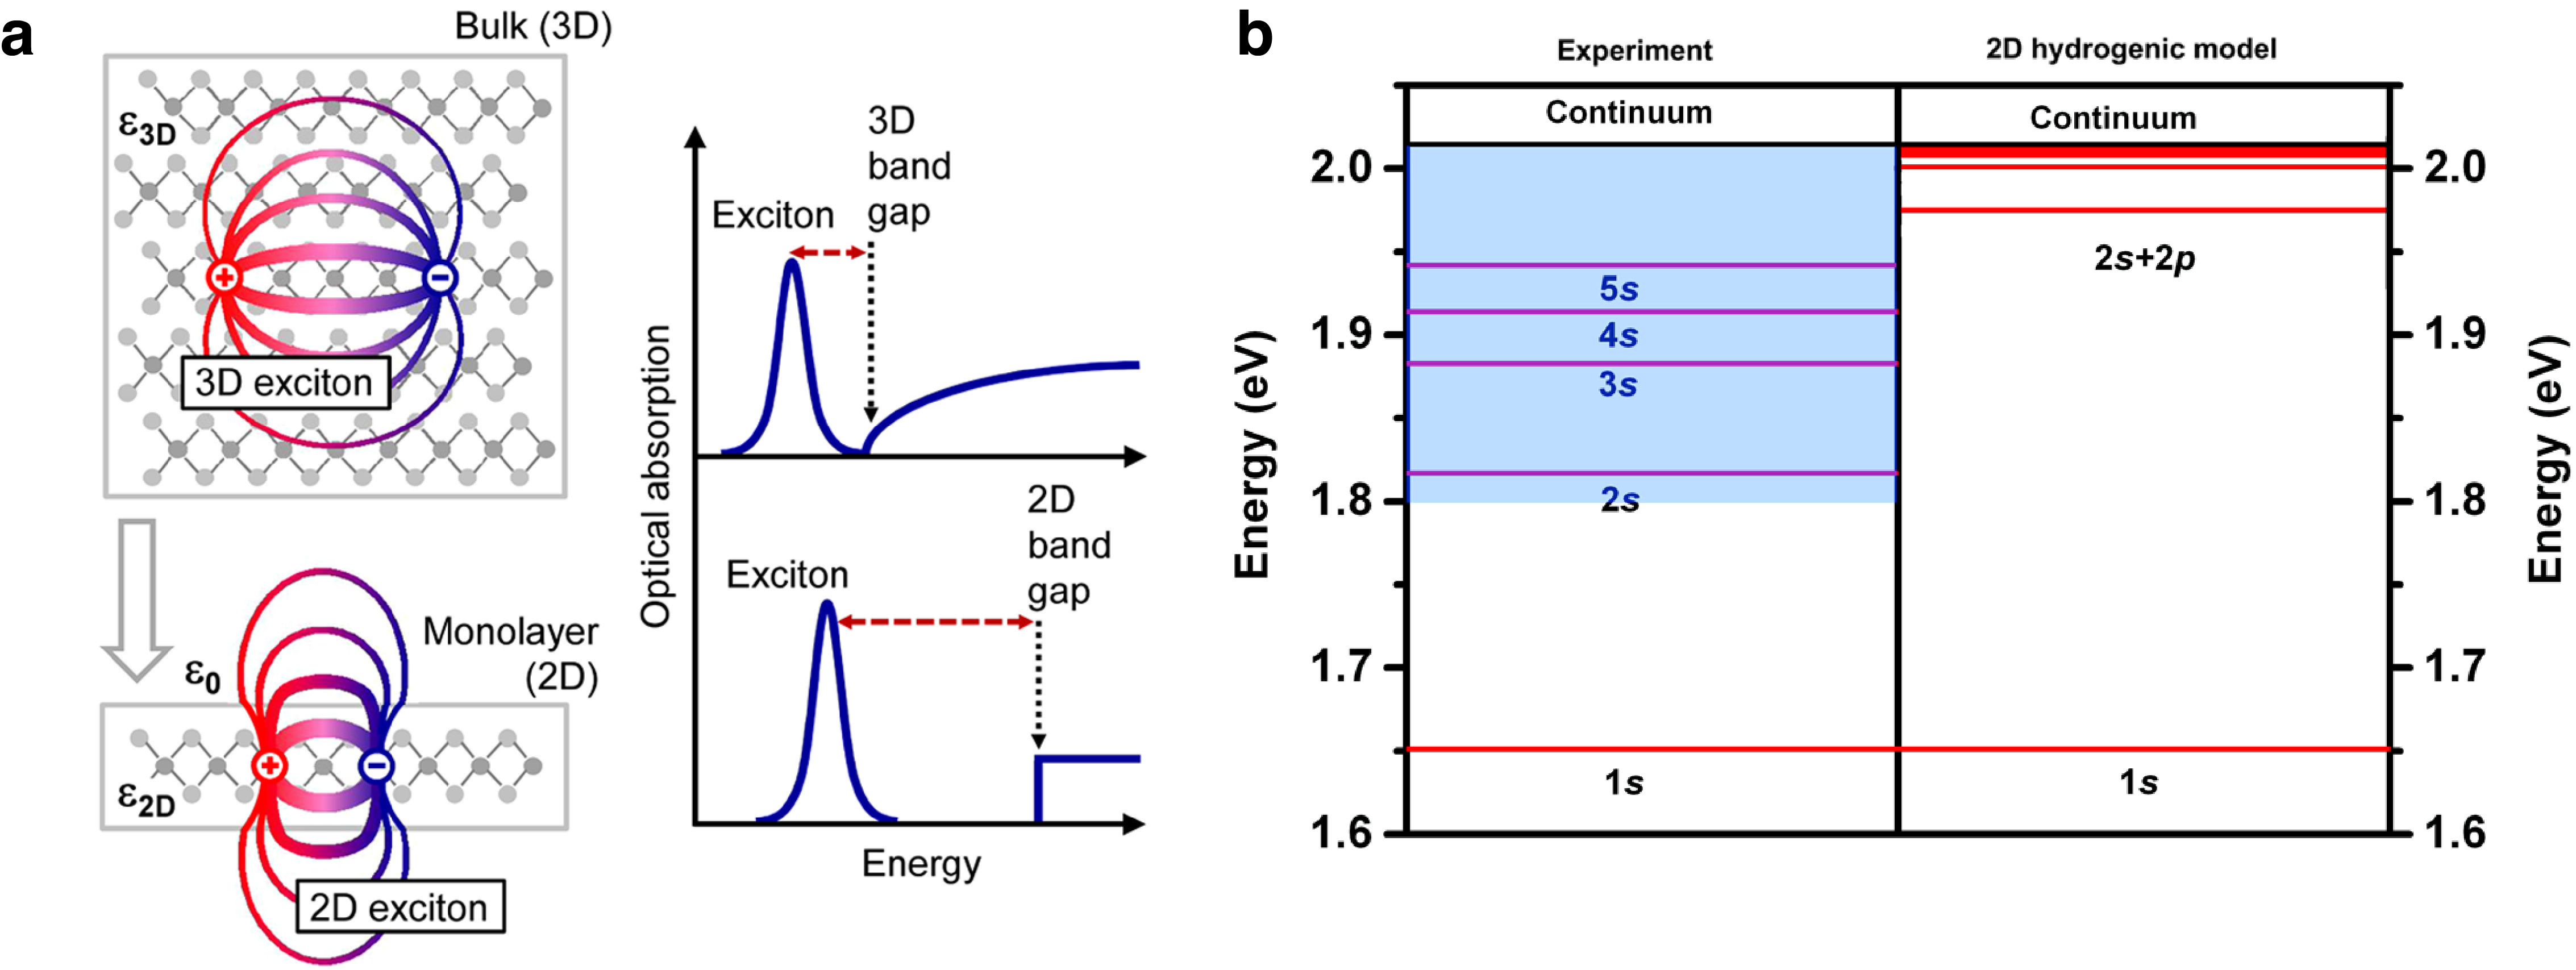
\includegraphics[width=1\textwidth]{Figures/C2/Fig.2-4_rydbergEx.jpg} 
\end{center}
\caption[Rydberg exciton states in 2D TMDCs] {\textbf{Rydberg exciton states in 2D TMDCs.} \textbf{a,}Schematic of the bound electron hole pairs in 3D and 2D. The reduced dielectric screening and 2d plane confinement increase the quasiparitcle bandgap and the exciton binding energy. 
\textbf{b,}Comparison of exciton energy from experiment and 2D hydrogen model. 
Red lines are exciton states obtained from one-photon absorption and blue shaded region is from two-photon absorption corresponding to the p-states.Figures are adpated from\cite{Chernikov2014-vo,He2014-ct}.}
\label{fig.rydberg_Ex}
\end{figure}
\end{quote}
\renewcommand{\baselinestretch}{2}
\small\normalsize
% --------------
However, the conventional Coloumb potential form fails to reproduce the experimentally observed binding energies and non-hydrogenic exciton spectra in TMDs (Figure~\ref{fig.rydberg_Ex}b).
This is due to the use of the constant dielectric constant $\varepsilon_r$ in the potential.
As in atomic thin layer, the electric field lines generated by an electron–hole pair extend partly within the 2D sheet and partly into the surrounding environment, which have a different permittivity\cite{Latini2015-za}.

By considering the nonlocal dielectric screening, the electron--hole
interaction can be more accurately described by the Rytova--Keldysh potential\cite{Keldysh1979-kr,Chernikov2014-vo}:
\begin{equation}
V_{\mathrm{eh}}(r) = -\frac{\pi e^2}{2 r_0} 
\left[ H_0\!\left(\frac{r}{r_0}\right) - Y_0\!\left(\frac{r}{r_0}\right) \right]
\label{eq:rytova}
\end{equation}
where $H_0$ and $Y_0$ are the Struve and Bessel functions, respectively.
$r_0$ is the screening length determined by the 2D polarizability and the surrounding dielectric environment(3 to 6 nm in TMD)\cite{Chernikov2014-vo}. 
At large electron--hole separations, $V_{eh}(r)$ scales in $1/r$ as the bare Coulomb interaction, while at shorter distances it exhibits a weaker $\log(r)$ dependence. 
Solving Eq.~\eqref{eq:wannier} with $V(r) = V_{\mathrm{eh}}(r)$ yields binding energies of several hundreds meV, consistent with experimental observations in monolayer MoS$_2$
and WSe$_2$.

In the presence of free carriers, excitons can interact with the surrounding Fermi sea of electrons or holes, forming new excitation states known as polarons\cite{Sidler2017-ff}. 
The polaron can be described as an exciton dressed by particle--hole excitations of the Fermi sea, shown as two different branches in the optical spectrum: an attractive polaron at lower energy and a repulsive polaron at higher energy\cite{Sidler2017-ff,Liu2021-er}.

\subsection{Exciton in external Electric field}
The motion of the exciton can be separated into two parts: the relative motion of the electron around the hole, which determines the binding energy and size of the exciton, and the center-of-mass (COM) motion of the exciton as a whole across the 2D plane of the material\cite{Yu2010-yp,Griffiths2019-oc}.
The corresponded coordinate is:
$\mathbf r = \mathbf r_e - \mathbf r_h$ for relative motion
and
$\mathbf R = (m_e \mathbf r_e + m_h \mathbf r_h)/(m_e+m_h)$ for the COM motion, where $m_e$ and $m_h$ are the electron and hole effective masses.
The total Hamiltonian can be expressed as:
\begin{equation}
H \;=\; H_{\mathrm{rel}}(\mathbf r) \;+\; H_{\mathrm{COM}}(\mathbf R).
\label{eq:exciton_split}
\end{equation}
The two respective Hamiltonian are:
\begin{align}
H_{\mathrm{rel}}(\mathbf r) &= -\frac{\hbar^2}{2\mu}\nabla_{\mathbf r}^2 
+ V(\mathbf r) \label{eq:H_rel}\\[6pt]
H_{\mathrm{COM}}(\mathbf R) &= -\frac{\hbar^2}{2M}\nabla_{\mathbf R}^2 
+ V_{\mathrm{ext}}(\mathbf R) \label{eq:H_COM}
\end{align}
Eq.~\ref{eq:H_rel} is also mentioned in eq.~\ref{eq:wannier}.
Solving this tells us how tightly the electron and hole are bound and what the size of the exciton is. 
Eq.~\ref{eq:H_COM} governs the COM motion of the exciton, with total mass $M = m_e + m_h$. 
When an external fields or potentials is involved, the exciton as a whole can be pushed around or trapped depending on the form of $V_{\mathrm{ext}}(\mathbf R)$. 
And the kinetic energy of the exciton can be defined as\cite{Yu2010-ae}:
\begin{equation}
E_{R}(k) = \frac{\hbar^{2}k^{2}}{2M}
\label{eq:exciton_Ek}
\end{equation}
With $\mathbf{k = k_n+k_p}$. $\mathbf{k_n}, \mathbf{k_p}$ refers to the electron and hole momentum, respectively.

An uniform electric field applied aligned with the TMD exciton couples directly to the electron--hole relative coordinate. 
In this case, the excitonic Hamiltonian includes an additional term, so that the Wannier equation becomes\cite{Pedersen2016-pv}:
\begin{equation}
\left[-\frac{\hbar^2}{2\mu}\nabla_{\mathbf r}^2 
- \frac{e^2}{4\pi\varepsilon_0\varepsilon_r |\mathbf r|}
+ e \epsilon \mathbf r \right] \varphi(\mathbf r) 
= E_r \varphi(\mathbf r),
\label{eq:wannier_field}
\end{equation}
where $\mu$ is the reduced mass and $\epsilon$ is the electrostatic field. 
In the weak-field regime, where the applied field is well below the dissociation threshold, the leading correction to the exciton energy is given by the quadratic Stark shift\cite{Lian2024-bh,Roch2018-lp}, then then energy shift of the 1s exciton depends on the field can be obtained in terms of\cite{Thureja2022-cv,Pedersen2016-pv}:
\begin{equation}
\Delta E \;=\; -\frac{1}{2}\,\alpha_{1s} \epsilon^2
\label{eq:stark_shift}
\end{equation}
where $\alpha$ is the 1s exciton polarizability.
Accroding to this, this electric field induced finite dipole moment can be expressed as $\alpha_{1s} \epsilon$. 
The exciton polarizability $\alpha$ is proportional to the exciton Bohr radius. 
% In our case, the external perturbation is an electric field with a Gaussian spatial profile:
% \begin{equation}
% E(\mathbf R) = E_0 \exp\!\left(-\frac{R^2}{2\sigma^2}\right),
% \label{eq:gaussian_field}
% \end{equation}
% where $E_0$ is the field amplitude and $\sigma$ is the characteristic width. 
% Because the exciton has a finite polarizability $\alpha$, this field produces an effective potential for the COM motion of the form
% \[
% V_{\mathrm{ext}}(\mathbf R) \;\propto\; -\alpha |E(\mathbf R)|^2.
% \]
% This means that the exciton experiences a trap whose shape follows the Gaussian profile of the applied field. 
% In physical terms, the exciton tends to move toward the region of strongest field, and if the field is localized, the exciton becomes confined in that region much like a particle in a potential well. 

% It is important to emphasize that the Wannier equation for the relative motion remains essential in this situation. 
% The internal solution determines key quantities such as the binding energy, dipole moment, and polarizability of the exciton. These parameters, in turn, set how strongly the exciton responds to the external field. 
% Without solving the Wannier equation, one would not know the size or strength of the exciton, and the description of its confinement would be incomplete. 
% Thus, the full picture combines both aspects: the internal exciton properties from $H_{\mathrm{rel}}$ and the COM dynamics under the external Gaussian field from $H_{\mathrm{COM}}$.

\subsection{Light-matter interaction}
The light-matter interaction can be described by the transition probabilities, which can be calculated through the Fermi'Golden rule\cite{Fox2010-ly}:
\begin{equation}
\Gamma \;=\; \frac{2\pi}{\hbar}\, \big|\langle f \vert H^{\prime} \vert i \rangle\big|^2 \,
\rho_{\mathrm{ph}}(\omega_n)
\label{eq:fermi_golden_rule}
\end{equation}
where $\Gamma$ is the radiative decay rate,$\langle f \vert H^{\prime} \vert i \rangle$ is the matrix element with the electric dipole interaction Hamiltonian $H^{\prime} = -e \mathbf{r} \cdot \mathbf{E}$.
$\lvert i\rangle$ and $\lvert f\rangle$ are the initial and final states, and $\rho_{\mathrm{ph}}(\omega_n)$ is the photonic density of states at the transition frequency. The matrix element is directly proportional to the oscillator strength $f_0$ as\cite{Fox2010-ly}:
\begin{equation}
f_0 \;=\; \frac{2 m_0 \omega_n}{\hbar}\,\big|\langle f \vert \mathbf{r}\cdot\mathbf{E} \vert i \rangle\big|^2 \
\label{eq:oscillator_strength}
\end{equation}
where $m_0$ is the free-electron mass, $\omega_n$ is the exciton transition frequency, $\hbar$ is the reduced Planck constant. 
In the 2D system,for exciton to absorb or emit a photon, the in-plane momentum must be conserved during the process.
A photon of frequency $\omega_n$ has wavevector magnitude
$q =\frac{\omega_n}{c}$ whose in-plane component $q_{\parallel}$ is small near normal incidence. 
An exciton with center-of-mass in-plane momentum $\mathbf K$ can couple directly to light only when its momentum matches the photon's in-plane momentum as $|\mathbf K| \;\le\; q_{\parallel}$.
This defines the light cone that a narrow disk around
$\mathbf K\!=\!0$ in momentum space\cite{Wang2018-my}. 
Excitons inside the light cone are optically bright and can absorb/emit photons efficiently, whereas excitons outside the cone are dark with respect to direct radiative processes and must first scatter (e.g., by phonons or disorder) back into the lightcone to recombine\cite{Paik2024-ip,}.

The exciton linewidth in directly related to the radiative decay rate, which is proportional to $1 / a_B^2$\cite{Wang2018-my}. Since TMD excitons have very small Bohr radius($\sim 1\,\ nm$), the calculated radiative broadening is on the order of 1 \cite{Glazov2015-us,Glazov2014-qz}.
This corresponds to ultrafast intrinsic lifetimes shorter than 1 ps\cite{Moody2015-iz,PhysRevB.93.205423}, which is about two orders of magnitude faster than excitons in GaAs quantum wells\cite{PhysRevLett.67.2355}. 
Additional broadening occurs from exciton--phonon scattering, intervalley relaxation, and disorder-induced inhomogeneity, which typically increase with temperature\cite{Cadiz2017-ly,Robert2018-if,Ajayi2017-ky,Moody2015-iz}.
Inhomogeneous broadening originates from spatial variations in the local environment, including disorder, strain, and dielectric fluctuations, which create a distribution of resonance energies across the sample\cite{Jakubczyk2019-wv}.
In TMD, exciton linewidths are often dominated by inhomogeneous broadening from disorder, strain, and dielectric fluctuations. 
Encapsulation in hBN provides a clean and uniform dielectric environment that suppresses these effects, allowing linewidths to approach the intrinsic homogeneous limit\cite{Jakubczyk2019-wv,Wang2018-my}.

% \subsection{Exciton-exciton interactions}
\section{Exciton polaritons in strong coupled microcavity system}
We have already discussed the Wannier-Mott excitons in the TMD system.
Polaritons in transition-metal dichalcogenide (TMD) systems are formed when strongly bound excitons interact with photons confined in an optical cavity\cite{Deng2010-ul}. 
The resulting strong coupling between exciton states and photon modes produces new hybrid quasiparticles that share properties of both.
Their large exciton binding energies and strong oscillator strengths enable robust polariton formation, even at elevated temperatures\cite{Liu2015-hm}.
The valley-selective optical response of TMD excitons further provides polaritons with spin–valley degrees of freedom\cite{LaMountain2021-ck,Chen2017-tc}.
These features make TMD polaritons a promising platform for studying nonlinear interactions and quantum photonic phenomena\cite{Gu2024-ul}.

\subsection{Planar microcavity system}
Polaritons are commonly studied in microcavities, where strong coupling between excitons and confined photons produces hybrid light–matter states\cite{Rahimi-Iman2020-tt,Deng2010-ul}. 
The planar (1D) microcavity is the simplest geometry, with confinement only along the growth direction while allowing in-plane propagation, making it well suited for examining dispersion and spatial transport. 
To realize this, a high quality-factor (Q) microcavity\cite{Vahala2003-yh} is essential, as it minimizes photon losses and prolongs the photon lifetime, thereby strengthening light–matter coupling and enhancing nonlinear polariton interactions\cite{Gu2021-cu,Emmanuele2020-oh,Louca2023-in,Datta2022-po,enhancing}. 

A Fabry–Pérot cavity with distributed Bragg reflectors (DBRs) provides simple, well-defined modes, making it ideal for polariton studies in 2D materials.
In this strcutrue, each DBR is formed by alternating two dielectric materials with a high refractive index contrast, with each layer thickness set to $l = \frac {\lambda}{4 n_0}$. 
For light with a vacuum wavelength $\lambda$ satisfying this condition, multiple reflections at the interfaces interfere constructively, resulting in high reflectivity.
Under this design, the DBR acts as a highly reflective mirror within a certain wavelength range, known as the stop band or photonic band. 
If we have the DBR with $N$ pairs of high-($n_2$) and low-($n_1$) refractive index layers, in the normal incidence case, the intensity reflectivity can be approximated by\cite{Rahimi-Iman2020-tt}:
\begin{equation}
  R \;=\;
  \left[
  \frac{ n_o \, n_2^{\,2N} \;-\; n_s \, n_1^{\,2N} }
       { n_o \, n_2^{\,2N} \;+\; n_s \, n_1^{\,2N} }
  \right]^2 
\label{eq:DBR_R}
\end{equation}
where $n_o$ is the refractive index of the incident medium, $n_1$ $n_s$ is the index of the substrate. 
\\The normalized stopband width around the central frequency
$f_0 = c/\lambda_0$ is:
\begin{equation}
  \frac{\Delta f_0}{f_0}
  \;=\;
  \frac{4}{\pi}\,\arcsin\!\left(\frac{n_2-n_1}{n_2+n_1}\right).
  \label{eq:DBR_bw}
\end{equation}\vspace{-0.5em}
Figure~\ref{fig.DBR} shows the simulated reflectance spectrum and the cross-section SEM of the bottom DBR we used in chapter 6. 
%Fig.5--------------
\renewcommand{\baselinestretch}{2}
\small\normalsize
\begin{quote}
\begin{figure}
\begin{center}
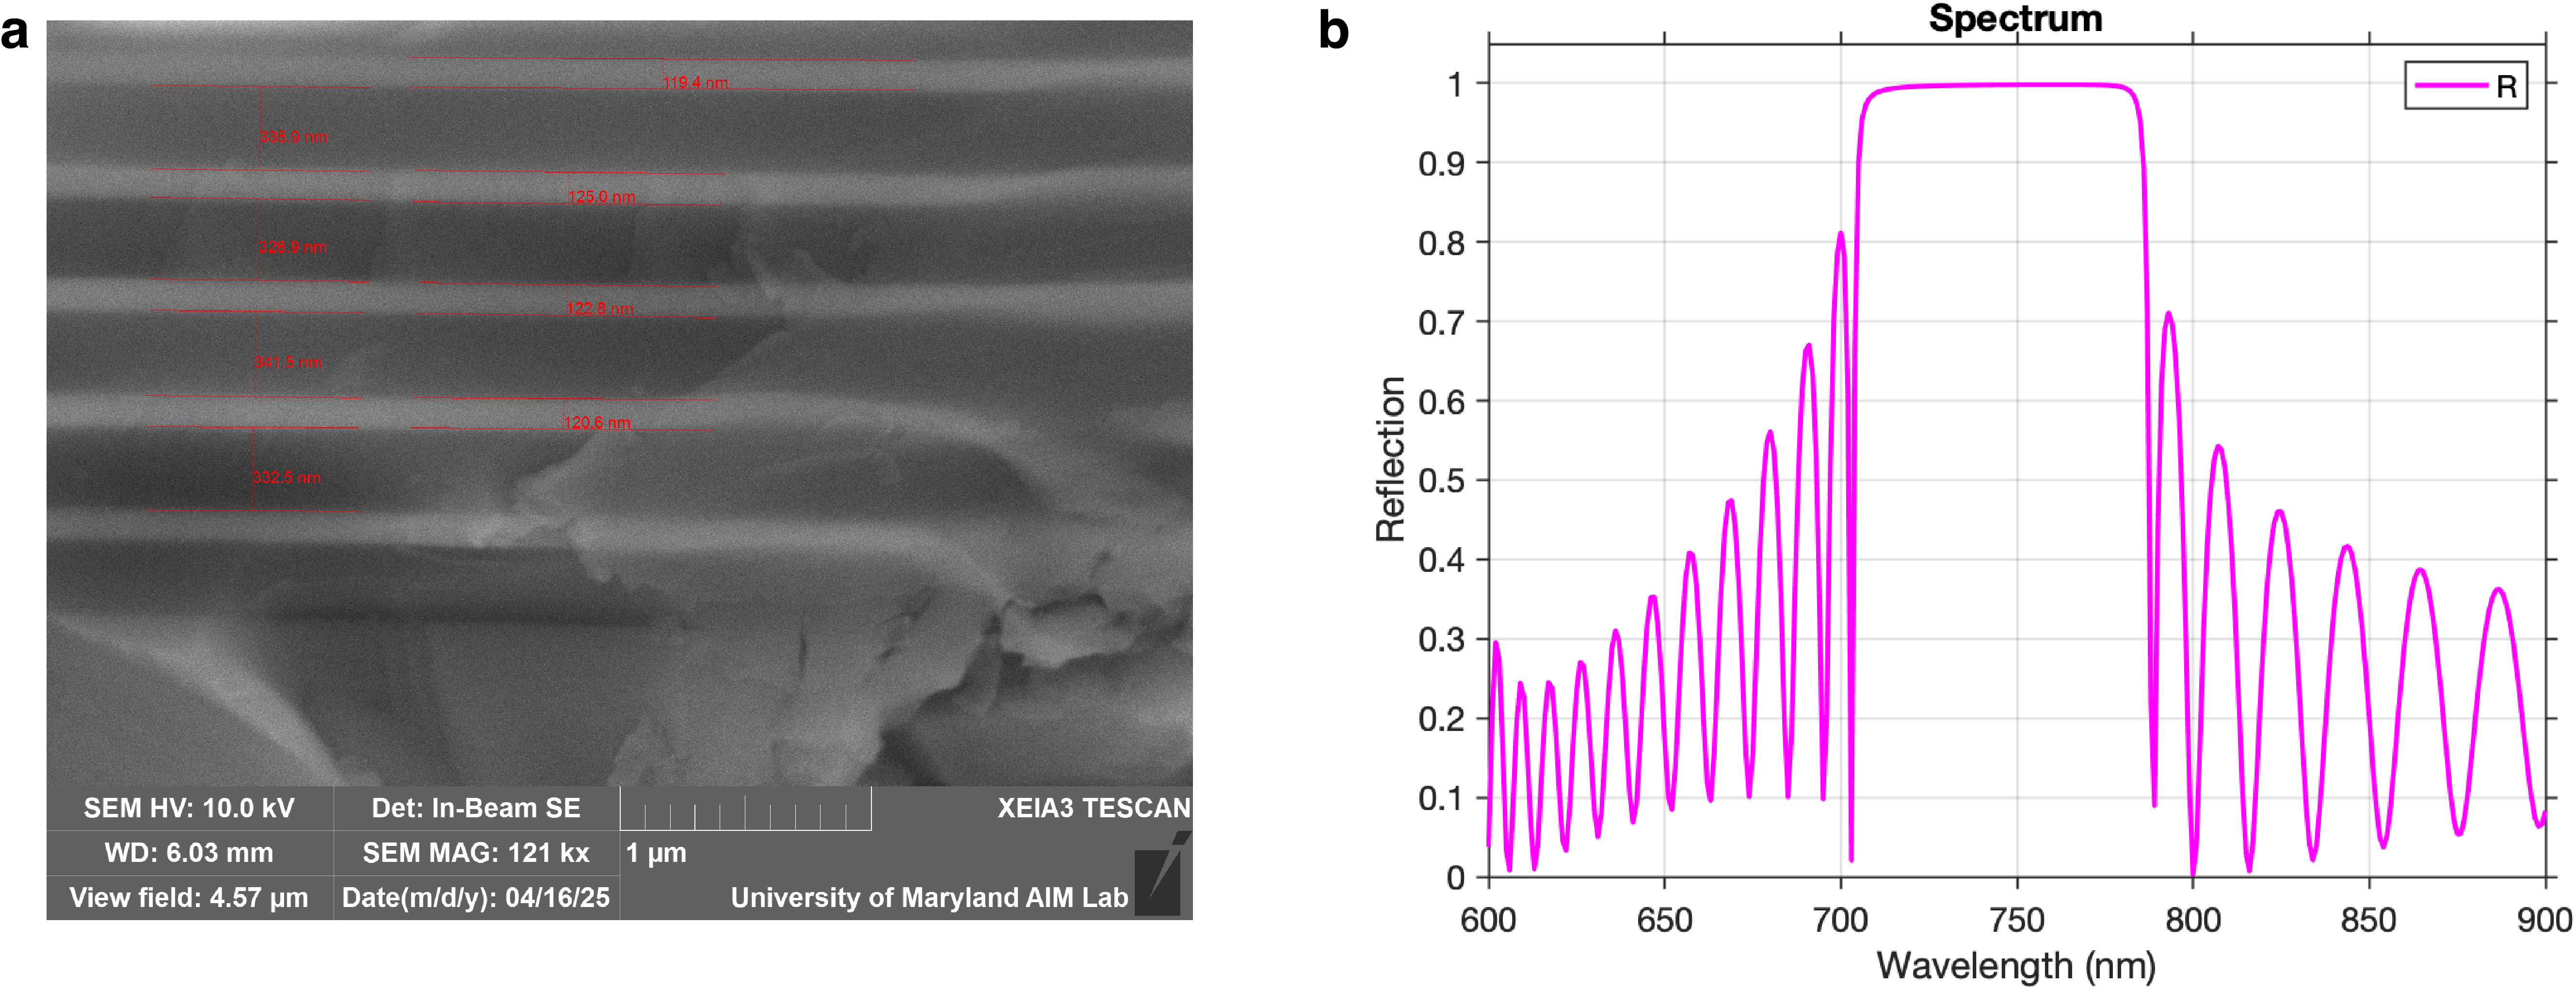
\includegraphics[width=0.9\textwidth]{Figures/C2/Fig.2-5_DBR.jpg} 
\end{center}
\caption[Structure of the sputtered DBR reviled by the cross section SEM and the reflectance spectrum calculated by TMM method.] {Structure of the sputtered DBR reviled by the cross section SEM \textbf{a} and the reflectance spectrum calculated by TMM method \textbf{b}.}
\label{fig.DBR}
\end{figure}
\end{quote}
\renewcommand{\baselinestretch}{2}
\small\normalsize
% --------
The cavity mode with the resonance at $\lambda_0$ can be formed by placing two DBRs with a separation corresponding to an optical thickness of $l_c = n\frac {\lambda}{2 n_0}$. Where $n$ is an integer. 
In this Fabry--P\'erot microcavity, the optical field is confined only in the $z$ direction but free in the $x$--$y$ plane. 
The distribution of the standing wave can be calculated by the transfer matrix method(see in Chapter 3). 

In the 1D microcavity, the cavity photon exhibits an in-plane energy dispersion as a function of the in-plane wavevector $k_{\parallel}$\cite{Deng2010-ul}:
\begin{equation}
E_{\mathrm{cav}} = \frac{\hbar c}{n_c} \sqrt{k_{\parallel}^2 + k_{\perp}^2},
\label{eq:cavity_dispersion}
\end{equation}
\vspace{-0.5em}
where the longitudinal wavevector is 
\vspace{-0.5em}
\begin{equation}
k_{\perp} = \frac{2\pi n_c}{\lambda}.
\label{eq:k_perp}
\end{equation}\vspace{-0.5em}
Given a photon incident angle $\theta$, the in-plane component of the wavevector can be approximated as:
\begin{equation}
k_{\parallel} \approx \frac{2\pi}{\lambda} \, \theta, 
\qquad \text{when } k_{\parallel} \ll k_{\perp}.
\label{eq:k_parallel}
\end{equation}\vspace{-0.5em}
Thus, the cavity energy can be expressed in a parabolic form as
\begin{equation}
E_{\mathrm{cav}} \approx \frac{\hbar c}{n_c} k_{\perp} 
+ \frac{\hbar^2 k_{\parallel}^2}{2 m_{\mathrm{cav}}},
\label{eq:cavity_parabola}
\end{equation}
where $m_{\mathrm{cav}}$ is the effective photon mass of the cavity mode.

\subsection{Strong coupling exciton polaritons}
The fundamental TE mode has its electric field within the cavity plane (transverse to $z$), matching the in-plane transition dipole of bright TMD excitons. 
According to the Fermi’s golden rule, the transition rate $\Gamma_{\omega}$ can be expressed as:
\begin{equation}
\Gamma(\omega)\;\propto\; \big|\langle X|\,(-\mathbf{d}\!\cdot\!\mathbf{E})\,|0\rangle\big|^{2}\,\rho(\omega)
= \big|\mathbf{d}\big|^{2}\,\big|\mathbf{E}\big|^{2}\,\kappa^{2}\,\rho(\omega),
\qquad \kappa \equiv \hat{\mathbf{d}}\!\cdot\!\hat{\mathbf{E}},
\end{equation}
Thus the alignment ($\kappa\!=\!1$) maximizes the $\Gamma$ for the TE mode.
where $\mathbf d$ is the exciton transition dipole, $\mathbf E$ is the cavity field at the monolayer, $\rho(\omega)$ is the photonic density of states, and $\kappa\equiv \hat{\mathbf d}\!\cdot\!\hat{\mathbf E}$ is the polarization (orientation) factor; TE polarization gives $\kappa\simeq 1$, whereas TM fields with an out-of-plane component reduce $\kappa$.
In cavity QED, the vacuum Rabi coupling for a single exciton to the cavity photon can be expressed by the coupling coefficient $g_1$ as:
\begin{equation}
g_1 \;=\; \frac{1}{\hbar}\,\big|\mathbf{d}\!\cdot\!\mathbf{E}_{\rm vac}\big|
\;=\; \frac{|\mathbf{d}|}{\hbar}\,\sqrt{\frac{\hbar\omega_c}{2\varepsilon_0 \varepsilon_b V_{\rm eff}}}\;\kappa,
\end{equation}
where $V_{\rm eff}\!\approx\!A\,L_{\rm eff}$ for a planar cavity, $\varepsilon_b$ is the background permittivity, and $\kappa$ is the polarization (orientation) factor. 
The effective cavity length $L_{\rm eff}$ consist of the cavity spacer length $L_{\rm eff}$ and the field penetration length $L_{\rm DBR}$, which is given by:
\begin{equation}
\ell_{\mathrm{eff}} = \frac{\lambda_0}{2}\,
\frac{n_{\mathrm{1}}\,n_{\mathrm{2}}}{\,n_0\,(\,n_{\mathrm{2}} - n_{\mathrm{2}}\,)} \, 
\end{equation}\vspace{-0.5em}
For the 2D exciton sheet, we assume there are $N$ numbers of exciotns within the mode area and can coherently couple to the cavity mode. 
This collective coupling strength can be expressed as:
\begin{equation}
g_{\rm 0} \;=\; \sqrt{N}\,g_1 \;\;\Rightarrow\;\;
\hbar\Omega_R \;=\; 2 g_{\rm 0}
\end{equation}\vspace{-0.5em}
The resulting hybrid light–matter quasiparticles are cavity polaritons. 
And when we looking at the exciton-polairton Hamiltonian, the microscopic coupling $g_{\rm 0}$ appears as the off-diagonal term at fixed in-plane wavevector $k_{\parallel}$:
\begin{equation}
\begin{aligned}
\hat H_{\mathrm{pol}}
&= \hat H_{\mathrm{cav}}+\hat H_{\mathrm{exc}}+\hat H_{\mathrm{int}} \\
&= \sum\!\
  E_{\mathrm{cav}}(k_\parallel)\,\hat a_{k_\parallel}^{\dagger}\hat a_{k_\parallel}
 +\sum\!\
  E_{\mathrm{exc}}(k_\parallel)\,\hat b_{k_\parallel}^{\dagger}\hat b_{k_\parallel}
 +\sum\!\
  g_0\big(\hat a_{k_\parallel}^{\dagger}\hat b_{k_\parallel}
         +\hat b_{k_\parallel}^{\dagger}\hat a_{k_\parallel}\big)
\end{aligned}\
\label{eq:H_polariton}
\end{equation}
where $\hat{a}^{\dagger}_{k_{\parallel}}$ ($\hat{b}^{\dagger}_{k_{\parallel}}$) creates a cavity photon (exciton) with in-plane wavevector $k_{\parallel}$, $E_{\mathrm{cav}}(k_{\parallel})$ and $E_{\mathrm{exc}}(k_{\parallel})$ are the bare dispersions, and $g_0$ is the light–matter coupling strength (enhanced by the cavity field and the excitonic oscillator strength).

In the strong-coupling regime (i.e., when the coherent coupling $g_0$ exceeds the relevant photon and exciton dissipation rates), the eigenmodes are coherent superpositions of the bare photon and exciton. 
The transformation to the lower/upper polariton operators is given by the Hopfield mixing:
\begin{equation}
\begin{pmatrix}
\hat{p}_{k_{\parallel}} \\
\hat{q}_{k_{\parallel}}
\end{pmatrix}
=
\begin{pmatrix}
C_{k_{\parallel}} & X_{k_{\parallel}} \\
X_{k_{\parallel}} & -\,C_{k_{\parallel}}
\end{pmatrix}
\begin{pmatrix}
\hat{a}_{k_{\parallel}} \\
\hat{b}_{k_{\parallel}}
\end{pmatrix},
\qquad
|C_{k_{\parallel}}|^{2}+|X_{k_{\parallel}}|^{2}=1,
\label{eq:Hopfield}
\end{equation}
where $|C_{k_{\parallel}}|^{2}$ and $|X_{k_{\parallel}}|^{2}$ quantify the photonic and excitonic fractions, respectively. It can be defined as:
\begin{equation}\
\lvert X_{k_\parallel}\rvert^{2}
= \frac{1}{2}\!\left(
1 + \frac{\Delta E(k_\parallel)}{\sqrt{[\Delta E(k_\parallel)]^{2}+4 g_0^{2}}}
\right)
\end{equation}

\begin{equation}\
\lvert C_{k_\parallel}\rvert^{2}
= \frac{1}{2}\!\left(
1 - \frac{\Delta E(k_\parallel)}{\sqrt{[\Delta E(k_\parallel)]^{2}+4 g_0^{2}}}
\right)
\end{equation}
Diagonalizing Eq.~\eqref{eq:H_polariton} yields the lower (LP) and upper (UP) polariton energies:
\begin{equation}
E_{\mathrm{LP,UP}}(k_{\parallel})
=
\frac{E_{\mathrm{cav}}(k_{\parallel}) + E_{\mathrm{exc}}(k_{\parallel})}{2}
\;\pm\;
\frac{1}{2}\sqrt{\big[E_{\mathrm{cav}}(k_{\parallel}) - E_{\mathrm{exc}}(k_{\parallel})\big]^2 + 4 g_0^{\,2}}\, 
\label{eq:LP_UP}
\end{equation}
From this we can see that when the cavity is on resonance with the exciton frequency (zero detuning), the energy splitting between the lower and upper polariton branch would be $2g_0$. This is also called the vacuum Rabi splitting.
The detuning between the uncoupled modes is defined as:
\begin{equation}
\Delta(k_{\parallel}) \;\equiv\; E_{\mathrm{cav}}(k_{\parallel}) - E_{\mathrm{exc}}(k_{\parallel}) .
\label{eq:detuning}
\end{equation}
At zero detuning ($\Delta=0$),the polaritons are half-light, half-matter ($|C_{k_{\parallel}}|^{2}=|X_{k_{\parallel}}|^{2}=1/2$).
%Fig.1-4--------------
\renewcommand{\baselinestretch}{1}
\small\normalsize
\begin{quote}
\begin{figure}
\begin{center}
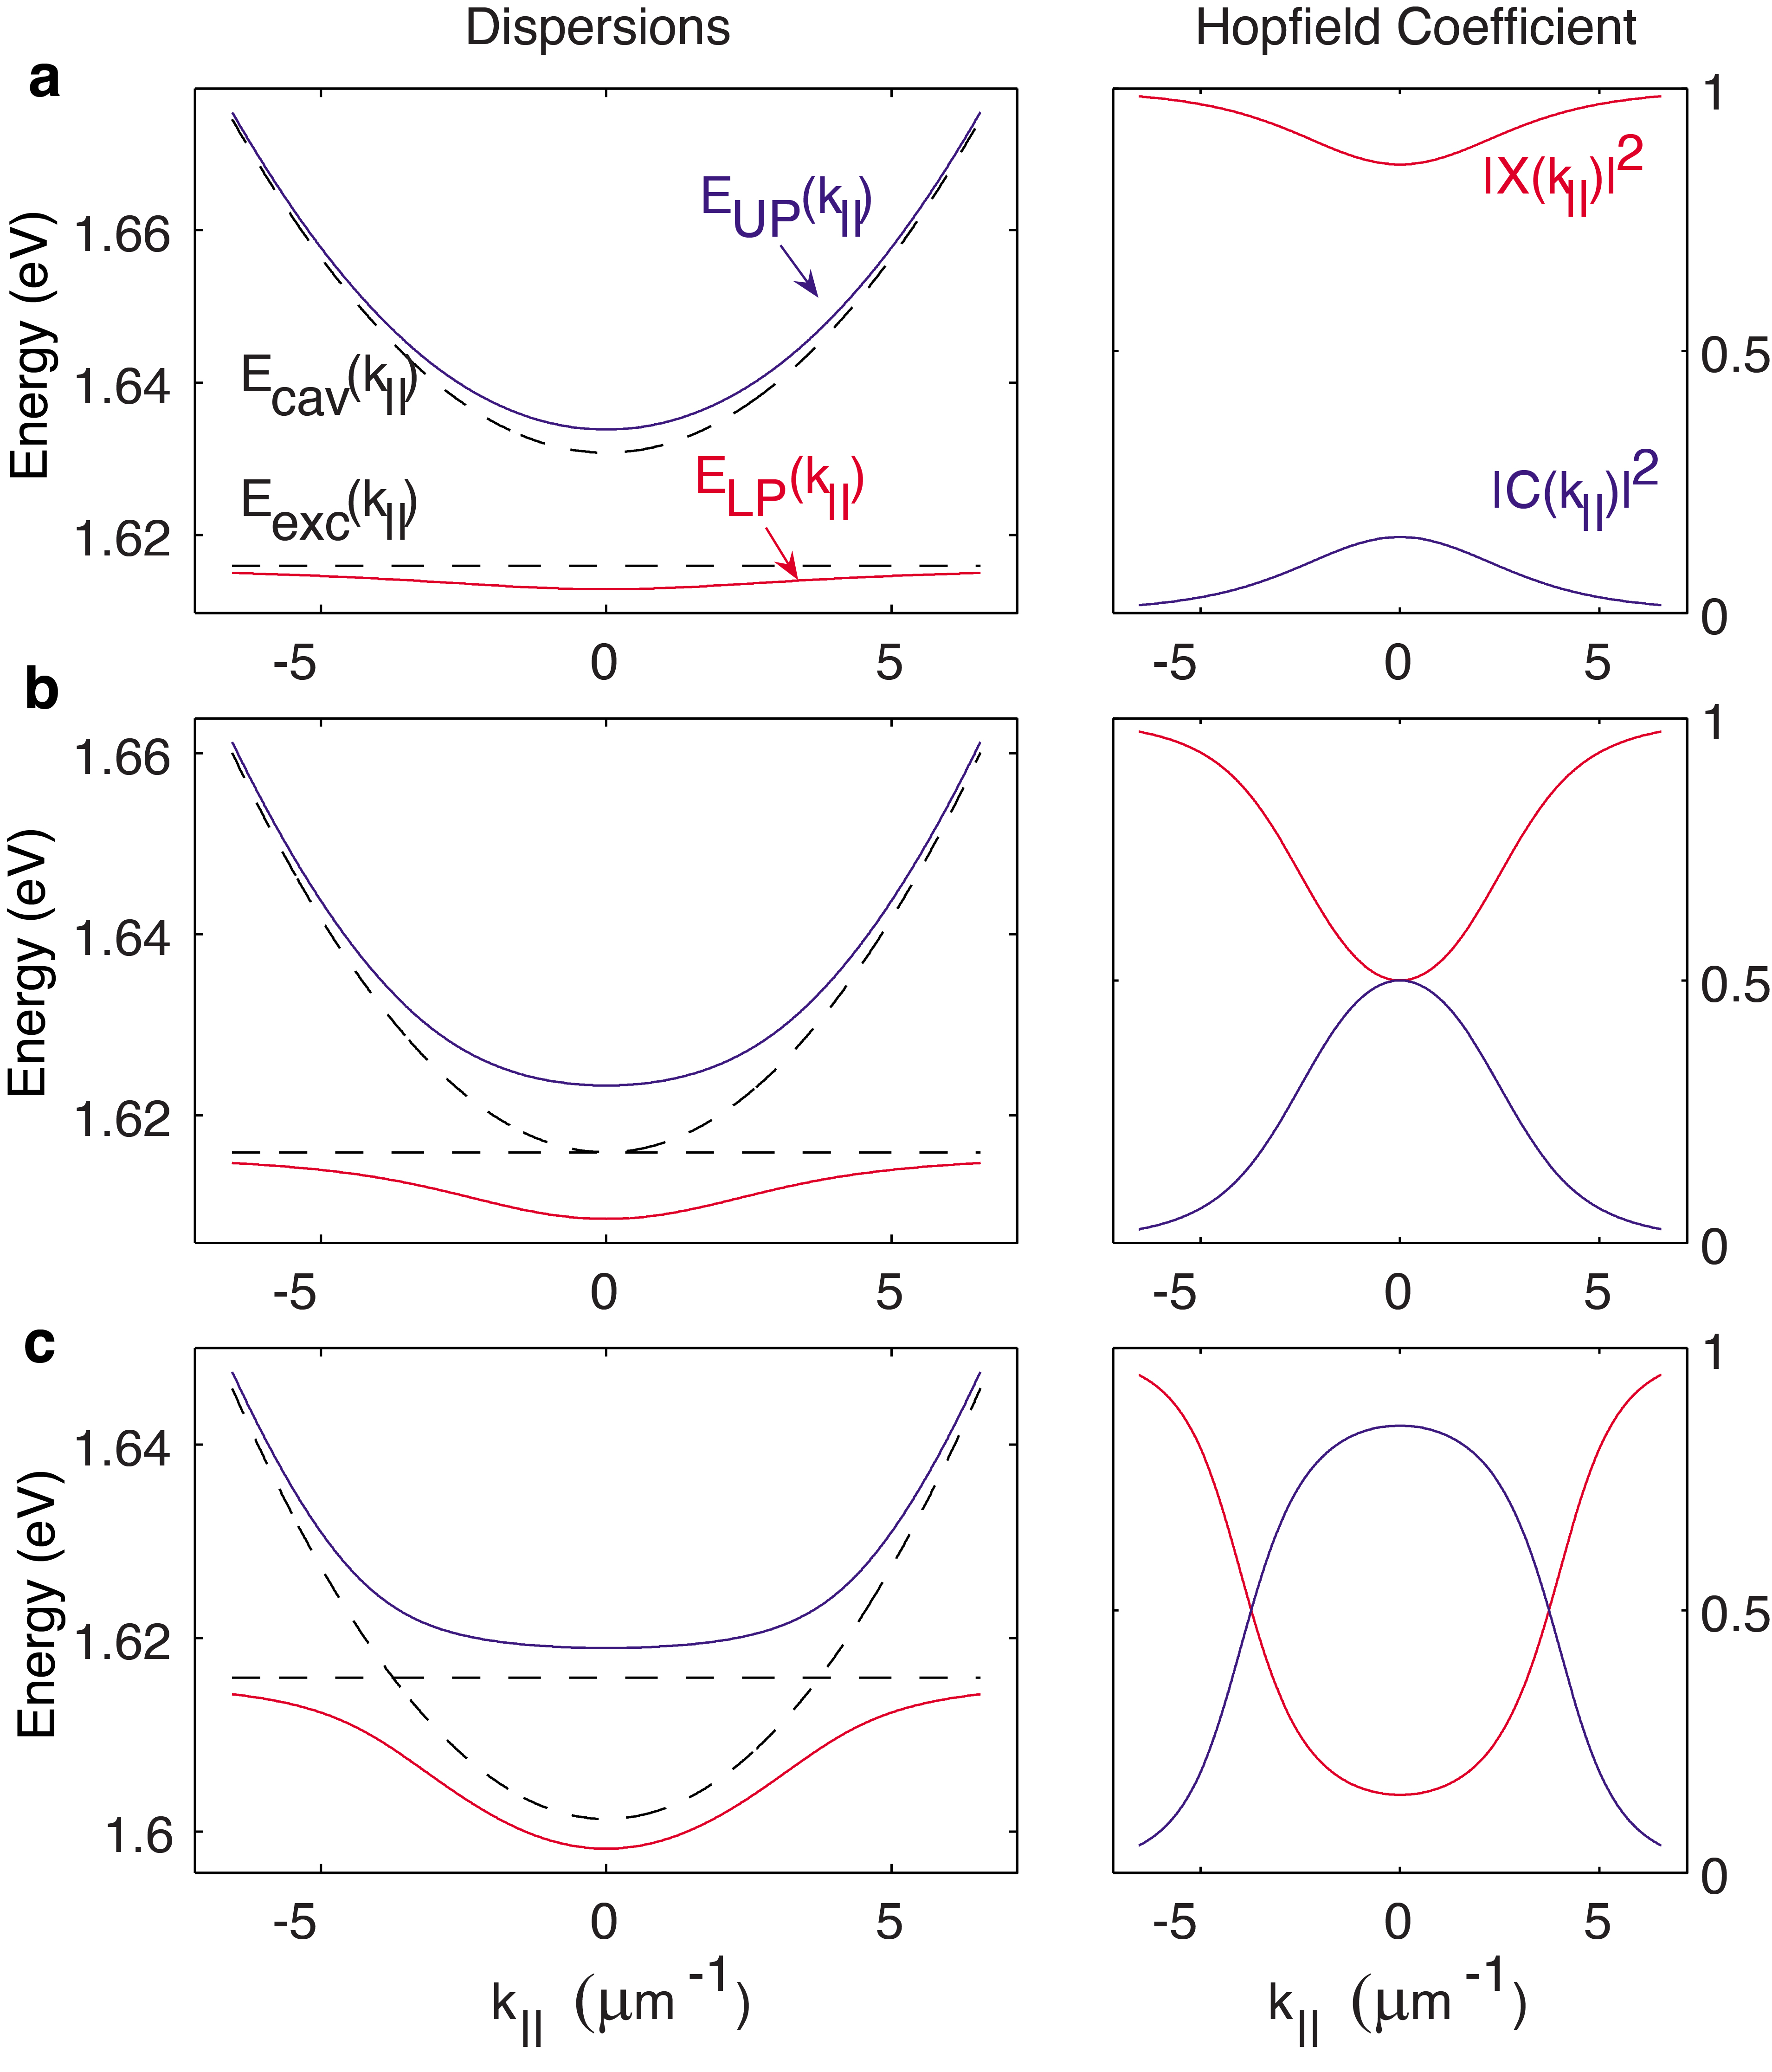
\includegraphics[width=0.8\textwidth]{Figures/C2/Fig.2-6_polariton_detune.jpg} % 
\end{center}
\caption[Exciton polariton dispersions and the Hopfield coefficent for lower polariton at different detuning $\Delta$] {\textbf{Exciton polariton dispersions and the Hopfield coefficent for lower polariton at different detunings.} \textbf{a,} $\Delta= 2 g_0$; \textbf{b,} $\Delta\ = 0$; \textbf{c,} $\Delta\ = -2g_0$.
Figures are adpated from[].}
\label{fig.rydberg_Ex}
\end{figure}
\end{quote}
\renewcommand{\baselinestretch}{2}
\small\normalsize
% --------------
Equivalently, using the 2D oscillator strength per area $f_{2\mathrm{D}}$, we can have the Rabi splitting as:
\begin{equation}
\Omega_R^{2} \;\propto\; \frac{f_{2\mathrm{D}}}{\varepsilon_b\,L_{\rm eff}}\,\kappa^{2}
\end{equation}
This shows that the in-plane TE polarization ($\kappa\!\approx\!1$) maximizes $\Omega_R$, and larger $f_{2\mathrm{D}}$ and smaller $L_{\rm eff}$ would further increase the Rabi splitting. 
Since the planar (1D) cavity provides an in-plane TE field aligned to the TMD intralayer exciton dipole, the dipole–field overlap $\lvert\mathbf d\!\cdot\!\mathbf E\rvert$ is maximized. 
Leveraging the monolayer’s large oscillator strength and the enhancement at the field antinode, the strong coupling regime is easy to access in the TMD embedded microcavity system, even with limited quality factor. 
The strong coupling is obtained when
\begin{equation}
2 g_{\rm 0} \;>\; \frac{1}{2}\big(\gamma_{\rm cav} + \gamma_{exciton}\big)
\end{equation}
where $\gamma_{\rm cav}$ and $\gamma_{exciton}$ are the cavity and exciton linewidths.
% \smallskip



%Chapter 3

\renewcommand{\thechapter}{3}

\chapter{Experimental Methods}
\label{chap3}

In this chapter, I present the fabrication and metrology methods employed throughout this thesis. 
Section~\ref{sec:van der Waals heterostructure Fabrication} describes the details of the fabrication process for dual-gate FET van der Waals heterostructure and outlines the basic electrostatic model.
Section~\ref{1D microcavity} introduces the transfer matrix method (TMM) simulations that will be used in Chapter~\ref{chap6}.
Section~\ref{sec:Metrology} discusses the working principle of Piezoresponse Force Microscopy (PFM) and the experimental details relevant to Chapter~\ref{chap4}. 
Finally, Section~\ref{sec:Optical Spectroscopy} presents the optical spectroscopy techniques employed to study exciton and polariton behavior.

\section{van der Waals heterostructure Fabrication} \label{sec:van der Waals heterostructure Fabrication}

\subsection{PC Dry transfer}
\label{sec:PC Dry transfe}
Since two-dimensional transition-metal dichalcogenides (TMDs) are layered crystals without dangling bonds between adjacent sheets, they can be mechanically exfoliated by the scotch-tape method down to the monolayer limit. 
The weak interlayer van der Waals forces also allow different 2D crystals to be stacked together, forming van der Waals heterostructures. 
Such heterostructures can be assembled either by wet or dry transfer. In the wet transfer process, exfoliated flakes are floated off the substrate in a liquid medium and redeposited onto a target, which is straightforward to implement but often leaves polymer residues or trapped bubbles at the interfaces. 
In contrast, dry transfer methods employ a polymer stamp (such as polycarbonate or polypropylene carbonate on a PDMS support) under an optical microscope to pick up and stack flakes sequentially. 
This deterministic “pick-up” approach enables accurate alignment, twist-angle control, and much cleaner interfaces, which are essential for studying the intrinsic electronic and optical properties of two-dimensional materials. 
For this reason, dry transfer was used throughout this work to assemble hBN-encapsulated TMD heterostructures.

In the PC-assisted dry transfer process, a thin polycarbonate (PC) film supported on a poly-dimethylsiloxane (PDMS) block is mounted on a transparent glass slide and integrated with a micromanipulator stage. 
Under an optical microscope, the PC/PDMS stamp is carefully lowered onto the target flake and brought into contact at a controlled temperature—typically 80–120 $^{\circ}$ for hBN and above 140 $^{\circ}$ for graphite. TMD flakes are usually picked up at lower temperatures to minimize defect activation and to reduce bubble and wrinkle formation caused by thermal expansion. 
The flake adheres to the polymer, and by sequentially picking up and releasing individual layers, van der Waals heterostructures are built up. After the full stack is assembled, it is released onto the final substrate at 140–160 $^{\circ}$. 
Once cooled to room temperature, the PC film with the chip is dissolved in chloroform for 10 minutes, followed by soaking in acetone and IPA for 10 minutes each. 
In addition to PC-based transfer, other polymers such as PPC are widely used because they can be released at lower temperatures and are easier to clean. 
Direct PDMS stamping without a polymer interlayer is also possible and offers a simpler workflow, though it tends to introduce more contamination and less reliable adhesion. 
Overall, the PC-assisted dry transfer method provides a balance of clean interfaces, mechanical stability, and reproducibility, and was therefore adopted in this work for the assembly of van der Waals heterostructures.

\subsection{Electrodes Patterning}
\label{sec:Electrodes Patterning}
Electron beam lithography (EBL) was employed to define nanoscale electrodes and contact pads for the van der Waals heterostructures in this thesis. 
In this technique, a finely focused electron beam is scanned across the surface of an electron-sensitive resist, directly writing the desired pattern with nanometer precision. 
For this work, the heterostructure samples were first spin-coated with a positive, low-molecular-weight e-beam resist, MMA(8.5) EL11(methyl methacrylate), at 3000 rpm for 60s, yielding a film thickness of approximately 500 nm. 
A second layer of high-molecular-weight resist, 495 PMMA A4, was then spin-coated at the same speed and time, producing a thickness of about 200 nm. 
This bilayer resist stack is particularly advantageous for metal lift-off, as the differential dissolution between MMA and PMMA creates an undercut profile that suppresses metal deposition on the sidewalls, thereby ensuring a clean and reliable lift-off process.
Before and after each spin-coating step, the samples were baked at 180 $^{\circ}C$ for 3 minutes to improve resist adhesion and remove residual solvent.
Patterning was performed using a field-emission electron-beam lithography Elionix ELS-G100 system operated at an acceleration voltage of 100 kV with beam currents of 1nA(for electrodes) and 50 nA (for lead pads). 
We used the SEM mode during the process to align the layout with the reference marker.
After exposure, the samples were developed in a 1:3 solution of DI water and isopropanol (IPA) for 1 minute.
Finally,the 5 nm Cr and 80 nm Au were deposited by thermal evaporation, and the remaining resist was lifted off in acetone and then soaked in IPA.

\subsection{Electrostatic Model in Dual-gate FET}
\label{Electrostatic Model in Dual-gate FET}
Stacking different 2D materials (eg. conductive graphite,insulated hBN, semiconductor TMD) together with a sequence enable multifunctional device. One of the most common device structure is the FETs (Field-Effect transistors).
In the 2D FET structure, a thin TMD flake is contacted by graphite, while a gate electrode is separated from the channel by insulating dielectric hBN. 
The graphite gate electrode does not conduct current directly into the TMD channel, instead, an applied gate voltage shifts the Fermi level in the TMD by electrostatic coupling. 
In this way, the carrier density in the channel can be tuned continuously from intrinsic to electron-doped or hole-doped regimes. 
A dual-gate geometry provides a large flexibility: the sum of the top-($V_{tg}$) and bottom-gate ($V_{bg}$) voltages controls the overall doping density, while the voltage difference establishes a vertical electric field($F_z$) across the TMD channel that modifies band alignment and excitonic energies.

Here, the electrostatic model we used for calculating the doping density $n_{total}$ and the applied electric field $F_z$ is shown in the schematic Fig.~\ref{fig.FET}.

%Fig.2--------------
\renewcommand{\baselinestretch}{1}
\small\normalsize
\begin{quote}
\begin{figure}
\begin{center}
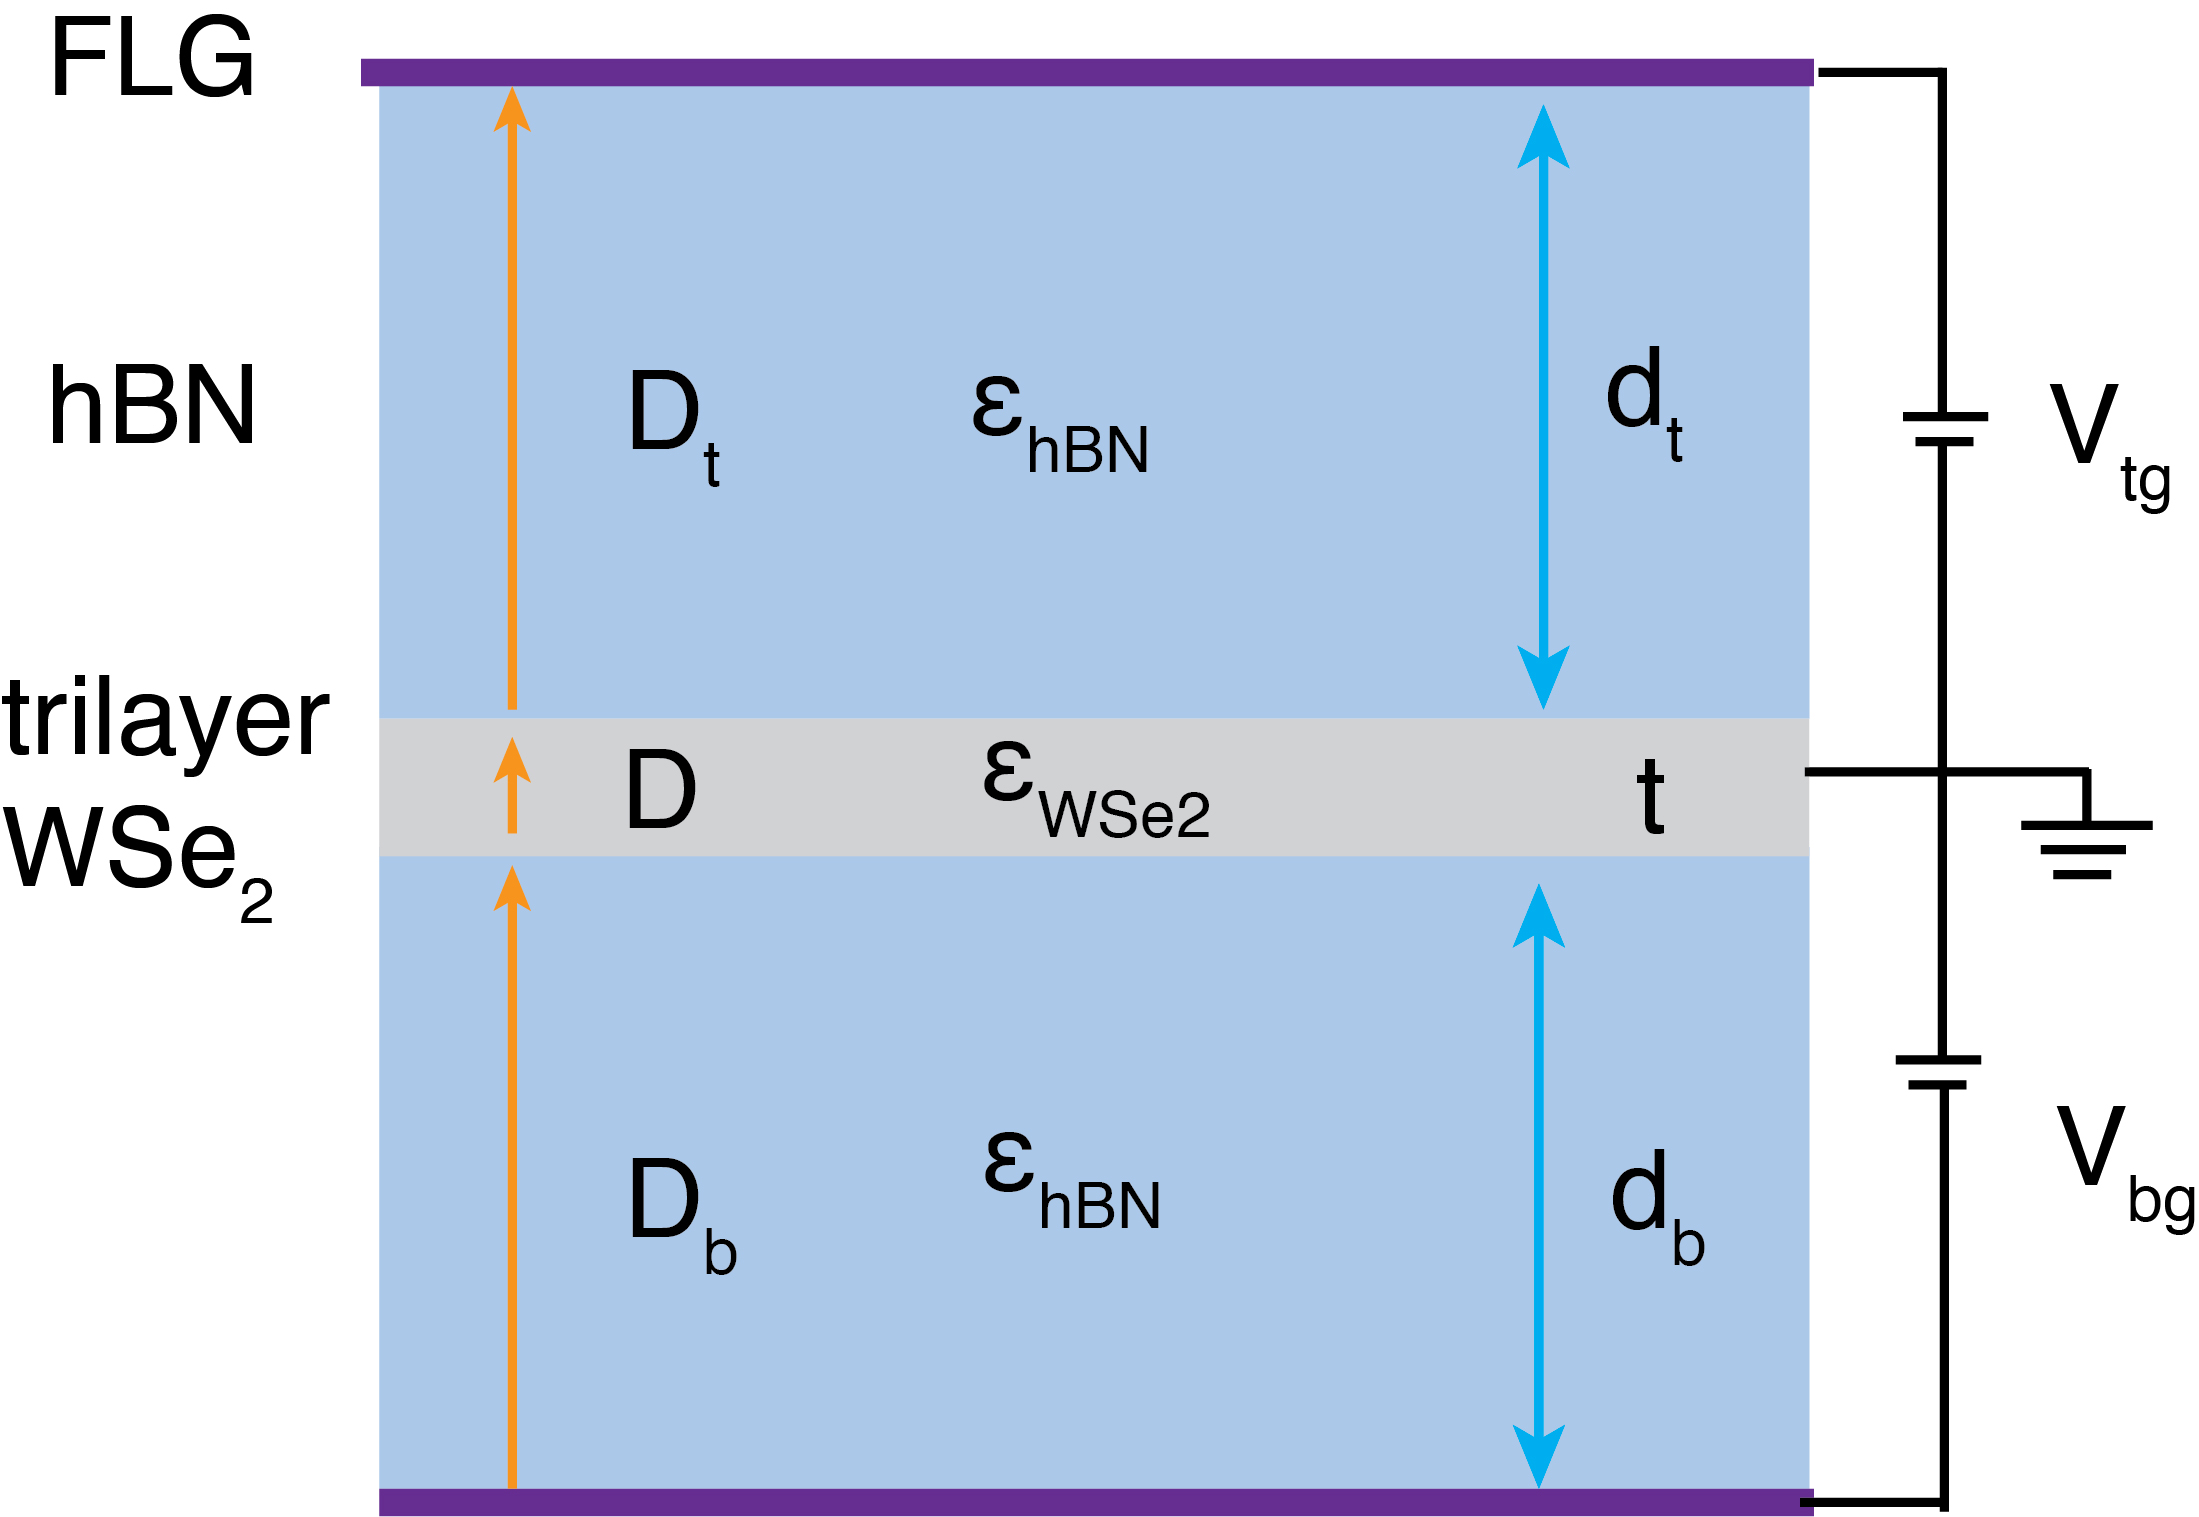
\includegraphics[width=0.45\textwidth]{Figures/C3/Fig.FET.jpg} % 
\end{center}
\caption[Schematic of the Dual-gate trilayer WSe$_2$ FET.] {\textbf{Schematic of the Dual-gate trilayer WSe$_2$ FET.}}
\label{fig.FET}
\end{figure}
\end{quote}
\renewcommand{\baselinestretch}{2}
\small\normalsize
% --------------

The TMD (here we use trilayer WSe$_2$ to keep it consistant with Chapter.5 )is modelled as the grounded sheet. 
Through the electrostatic gating, the generated displacement field $D_t$ and $D_b$ according to the applied $V_{tg}$ and $V_{bg}$ can lead to the net carrier doping in the TMD layer with the density of $n_{total}$ and the displacement filed $D_z$. 
These two parameters can be tunded independently through $V_{tg}$ and $V_{bg}$. The displacement field can be tuned as:
\begin{align}
D_T = C_{top} \bigl(V_{tg} - V^0_{tg}\bigr)  \label{eq:Dfield_t} \\ D_B = -C_{bot} \bigl(V_{bg} - V^0_{bg}\bigr)
\label{eq:Dfield_b}
\end{align} 
where the $V^0_{tg}$ and $V^0_{bg}$ are the voltage needed to compensate the initial environmental doping.
Then we can have the description of the top and bottom capacitance per unit area as:
\begin{align}
C_{top} = \frac{\epsilon_{0}\epsilon_{hBN}}{d_{t}} \label{eq:Ctop} \\
\quad  C_{bot} = \frac{\epsilon_{0}\epsilon_{hBN}}{d_{b}} \label{eq:Cbot}
\end{align} 
where the $d_{t}$ and $d_{b}$ are the thickness of the top and bottom encapsulated hBN, respectively.$\epsilon_{0}$ refers to the vacuum permittivity and .$\epsilon_{hBN}$ is the hBN dielectric constant, which we use a value of 3.7 for all the estimation. 
Now, we can obtain the electron density with the parallel capacitor model:
\begin{align}
n_{\text{total}} &= n_{top} + n_{bot} = \frac{1}{e} \left[ C_{top} \left( V_{tg} - V^{0}_{tg} \right) 
+ C_{bot} \left( V_{bg} - V^{0}_{bg} \right) \right] \label{eq:chargeQ}
\end{align}
As a result, we can calculate the total doping density inside the TMD by plug Eq.~\ref{eq:Ctop},\ref{eq:Cbot} into \ref{eq:chargeQ}, Finally, the net carrier doping density can be calculated as
\begin{equation}
n_{\text{total}} = \frac{1}{e}\,\epsilon_{0}\epsilon_{hBN} 
\left[ \frac{ V_{tg} - V^{0}_{tg} }{d_t}
     + \frac{ V_{bg} - V^{0}_{bg} }{d_b} \right]
\label{eq:ntotal}
\end{equation}
Then, we can calculate the displacement field $D$ accross the TMD induced through the gating (assuming there are no charges in TMD layer)
\begin{align}
\begin{split}
D &= \frac{1}{2} \left( D_{tg} + D_{bg} \right) \\
  &= \frac{1}{2}\,\epsilon_{0}\epsilon_{hBN} 
     \left[ \frac{ V_{tg} - V^{0}_{tg} }{d_t} 
          - \frac{ V_{bg} - V^{0}_{bg} }{d_b} \right]
\end{split}
\label{eq:Fieldtotal}
\end{align}
Finally, the applied electric field $F_z$ is calculated as:
\begin{align}
\begin{split}
F_z &= \frac{1}{2}\,\frac{\epsilon_{hBN}}{\epsilon_{TMD}}
     \left[ \frac{ V_{tg} - V^{0}_{tg} }{d_t} 
          - \frac{ V_{bg} - V^{0}_{bg} }{d_b} \right]
\end{split}
\label{eq:Efield}
\end{align}
The $\epsilon_{TMD}$ we use for trilayer WSe$_2$ is around 7 in \ref{chap5}.

\section{1D microcavity}
\label{1D microcavity}

\subsection{Transfer Matrix Method}
\label{Transfer Matrix Method}
The transfer matrix method (TMM) is a widely used approach for modeling the optical response of multilayer thin-film structures. 
In this method, each dielectric layer is treated as a homogeneous medium characterized by its refractive index and thickness. 
Light propagation through a layer is represented by a propagation (phase) matrix, while each interface between adjacent layers is described by a dynamical matrix derived from the Fresnel reflection and trans-mission coefficients. 
By multiplying the matrices of all layers, one obtains a global transfer matrix that directly relates the incident and transmitted electromagnetic field amplitudes, from which the reflectance, transmittance, and absorption spectra can be calculated.  

To illustrate the method, consider a three-medium system with refractive indices $n_0$, $n_1$, and $n_2$, where the middle film has thickness $L$ as shown in the Fig.~\ref{fig.TMM}.

%Fig.3--------------
\renewcommand{\baselinestretch}{1}
\small\normalsize
\begin{quote}
\begin{figure}
\begin{center}
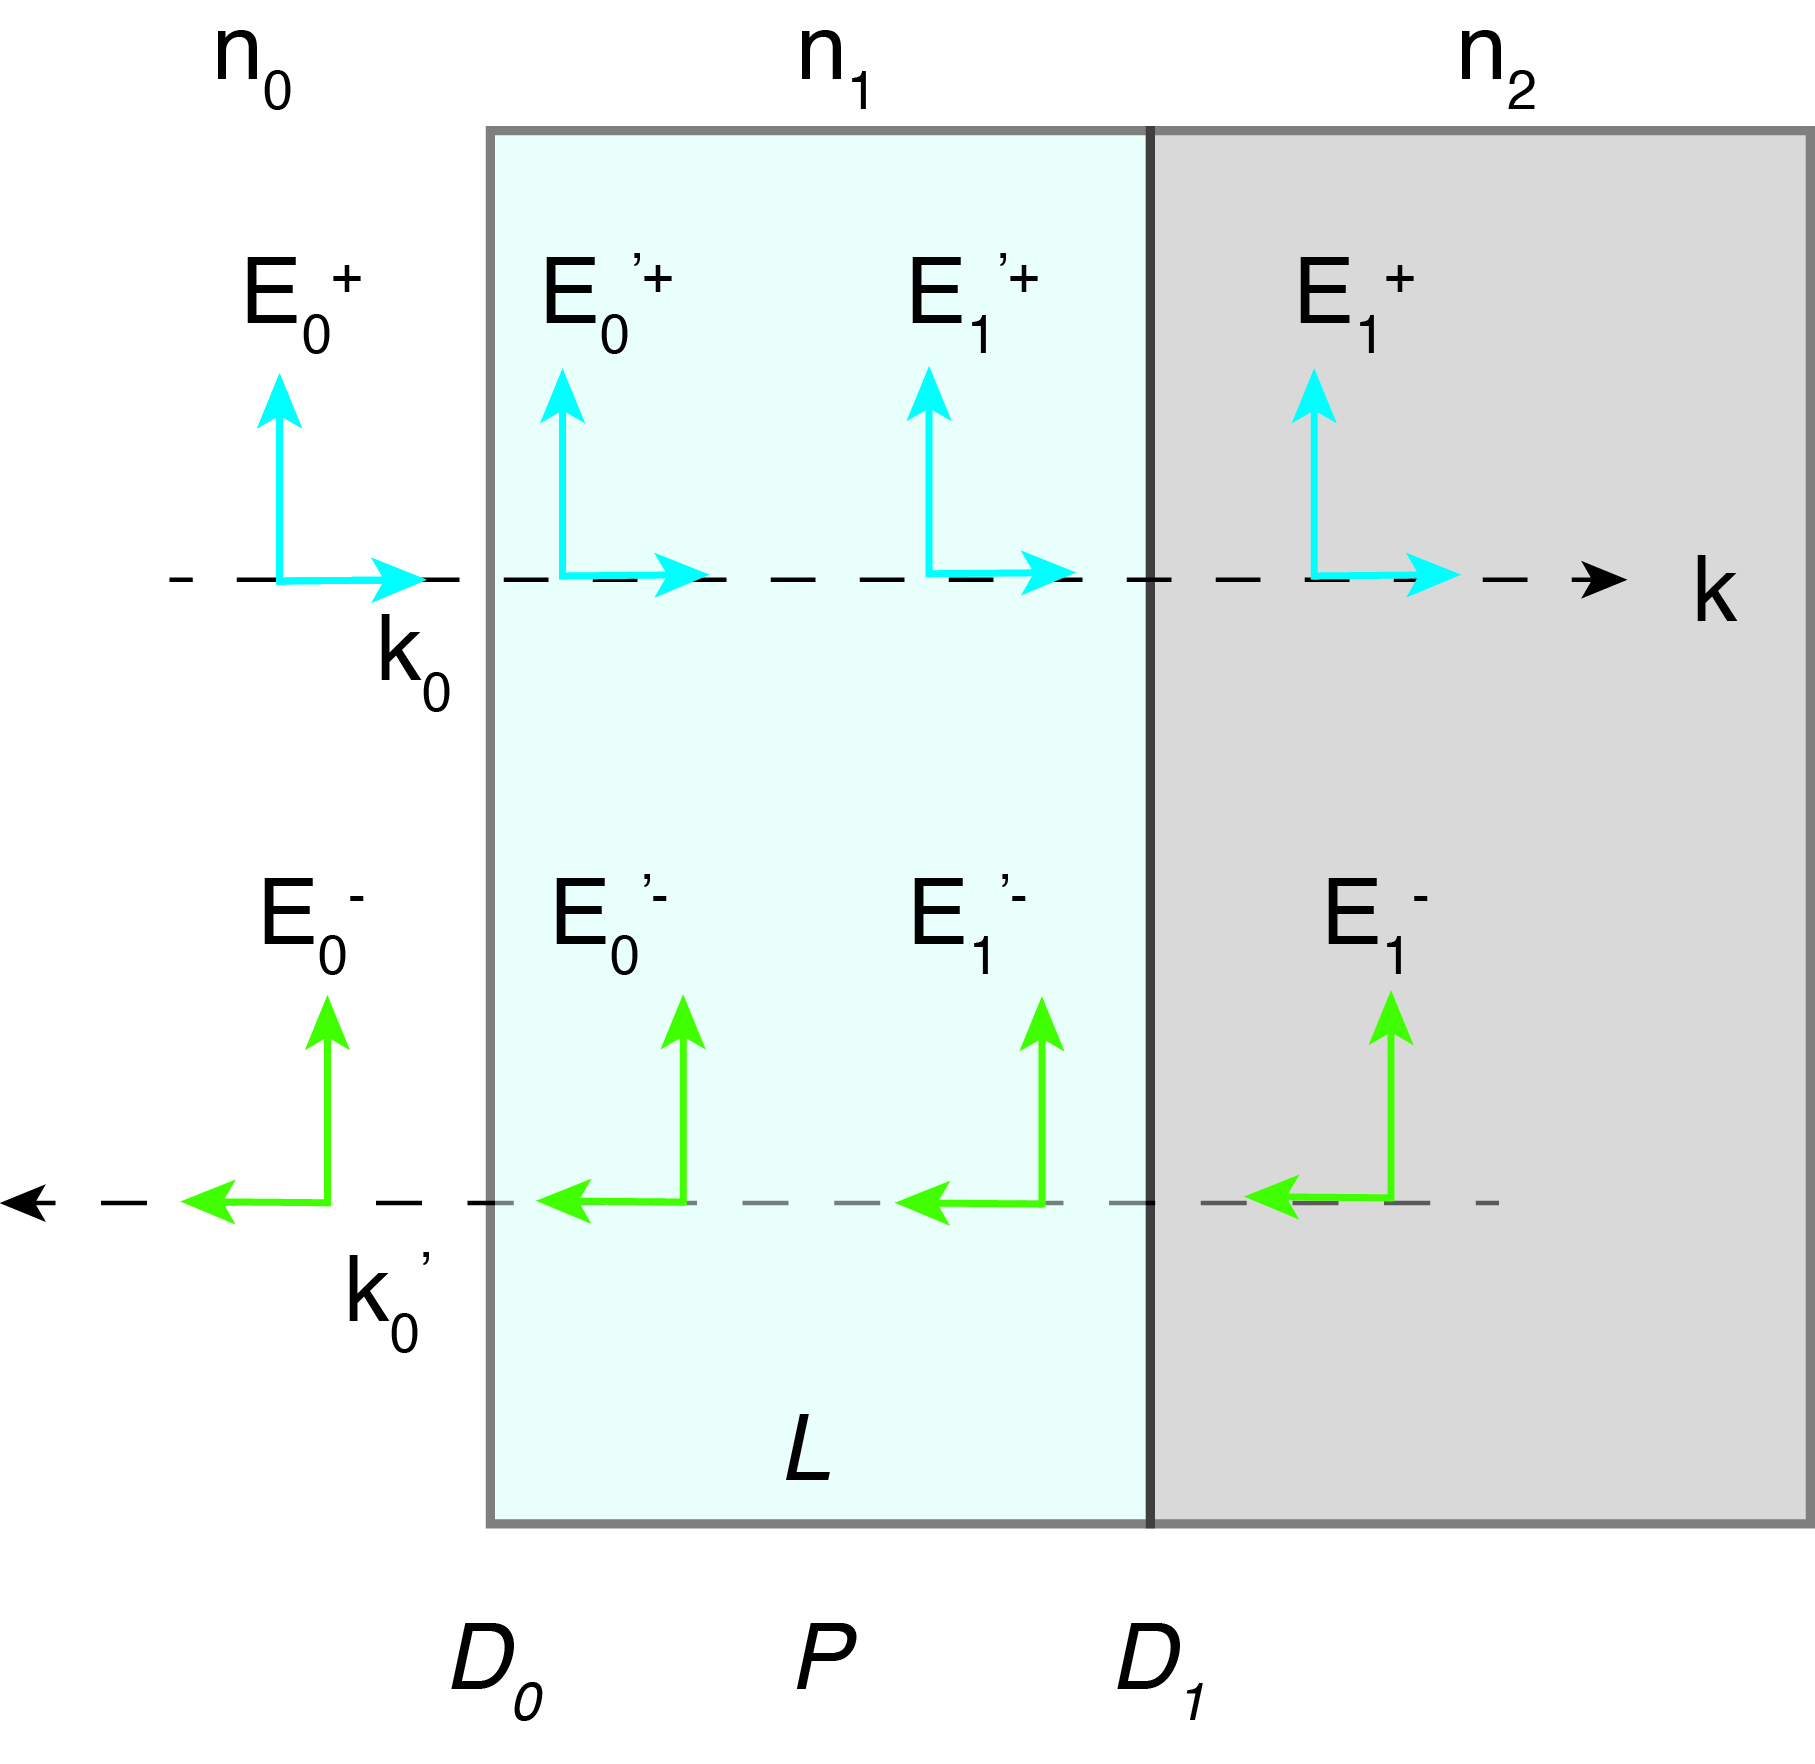
\includegraphics[width=0.4\textwidth]{Figures/C3/Fig.TMM.jpg} % 
\end{center}
\caption[Schematic of the layered structure with propagating wave's electric field and wave vector.] {Schematic of the layered structure with propagating wave's electric field and wave vector.The thickness of the dielectric materials is set as L}
\label{fig.TMM}
\end{figure}
\end{quote}
\renewcommand{\baselinestretch}{2}
\small\normalsize
% --------------

For TE (s-polarized) light, the vacuum wavenumber is $k_0 = 2\pi/\lambda$ and the longitudinal wavevector component in each medium is defined as
\begin{equation}
q_j = k_0 n_j \cos\theta_j, 
\qquad j \in \{0,1,2\},
\label{eq:q_def}
\end{equation}
with the angles $\theta_j$ constrained by Snell’s law,
\begin{equation}
n_0 \sin\theta_0 = n_1 \sin\theta_1 = n_2 \sin\theta_2.
\label{eq:snell}
\end{equation}

The electric field in each region can then be expressed as a superposition of forward- and backward-propagating plane waves:
\begin{equation}
E(x)=
\begin{cases}
E_0^{+} e^{i k_0 x} + E_0^{-} e^{-i k_0 x}, & \text{for } x<0,\\[4pt]
E_1^{+} e^{i k_1 x} + E_1^{-} e^{-i k_1 x}, & \text{for } 0<x<L,\\[4pt]
E_2^{+} e^{i k_2 (x-L)} + E_2^{-} e^{-i k_2 (x-L)}, & \text{for } x>L.
\end{cases}
\label{eq:Ex_f}
\end{equation}
By enforcing continuity of the electric field and its derivative at each interface, one obtains the Fresnel reflection and transmission amplitudes for TE polarization:
\begin{equation}
r_{ij}^{(\mathrm{TE})} = \frac{q_i - q_j}{q_i + q_j}, 
\qquad
t_{ij}^{(\mathrm{TE})} = \frac{2 q_i}{q_i + q_j}.
\label{eq:fresnel}
\end{equation}

These amplitudes are then used to construct the dynamical matrices. 
At the left interface ($n_0|n_1$) and right interface ($n_1|n_2$), the relations take the form
\begin{equation}
D_0 = \frac{1}{t_{01}}
\begin{pmatrix}
1 & r_{01} \\
r_{01} & 1
\end{pmatrix}, 
\qquad
D_1 = \frac{1}{t_{12}}
\begin{pmatrix}
1 & r_{12} \\
r_{12} & 1
\end{pmatrix}.
\label{eq:D_matrices}
\end{equation}

Propagation inside the film of thickness $L$ is described by a diagonal matrix that accounts for the phase shift $\delta = q_1 L$ of forward and backward waves:
\begin{equation}
P =
\begin{pmatrix}
e^{+i\delta} & 0 \\
0 & e^{-i\delta}
\end{pmatrix}.
\label{eq:P_matrix}
\end{equation}

The total transfer matrix of the structure is obtained by combining the interface and propagation matrices as
\begin{equation}
T = D_1 P D_0 =
\begin{pmatrix}
A & B \\
C & D
\end{pmatrix},
\qquad
\begin{pmatrix}
E_1^{+} \\
E_1^{-}
\end{pmatrix}
=
T
\begin{pmatrix}
E_0^{+} \\
E_0^{-}
\end{pmatrix}.
\label{eq:T_matrix}
\end{equation}
Explicitly, the matrix elements are
\begin{align}
A &= \frac{e^{+i\delta} + r_{12} r_{01} e^{-i\delta}}{t_{12} t_{01}}, &
B &= \frac{r_{01} e^{+i\delta} + r_{12} e^{-i\delta}}{t_{12} t_{01}}, \label{eq:AB_elements}\\[6pt]
C &= \frac{r_{12} e^{+i\delta} + r_{01} e^{-i\delta}}{t_{12} t_{01}}, &
D &= \frac{r_{12} r_{01} e^{+i\delta} + e^{-i\delta}}{t_{12} t_{01}} .
\label{eq:CD_elements}
\end{align}

Finally, the reflection and transmission amplitudes can be obtained by applying the boundary condition that no wave is incident from the right-hand side ($E_1^- = 0$). 
This leads to
\begin{equation}
r = \frac{E_0^-}{E_0^+} = -\frac{C}{D},
\qquad
t = \frac{E_1^+}{E_0^+} = \frac{\det T}{D} = \frac{q_2/q_0}{D}.
\label{eq:rt}
\end{equation}
The measurable reflectance and transmittance are then
\begin{equation}
R = |r|^2,
\qquad
T = \frac{\mathrm{Re}(q_2)}{\mathrm{Re}(q_0)} |t|^2,
\qquad
A = 1 - R - T.
\label{eq:RTA}
\end{equation}

\subsection{Distributed Bragg Reflector(DBR)}
\label{Distributed Bragg Reflector(DBR)}
A high quality-factor (Q) microcavity is essential to minimize photon losses and extend the photon lifetime, thereby enhancing the light-matter coupling strength and nonlinear interactions among polaritons. 
A Fabry–Pérot cavity composed of distributed Bragg reflectors (DBRs) offers simple, well-defined optical modes that are easy to model and measure, making it particularly suitable for polariton studies in 2D materials. 
Each DBR is formed by alternating two dielectric materials with a high refractive index contrast, with each layer thickness set to $l = \frac {\lambda}{4 n_0}$ to achieve constructive interference and high reflectivity within the stopband. 
Placing two DBRs with a separation corresponding to an optical thickness of $l_c = \frac {\lambda}{2 n_0}$ forms a resonance at $\lambda_0$.

\section{Metrology}
\label{sec:Metrology}

\subsection{PFM}
Piezoresponse Force Microscopy (PFM) is an atomic force microscopy–based technique for characterizing piezoelectric and ferroelectric materials at the nanoscale. 
In PFM, a conductive AFM tip is brought into contact with the sample surface, and an AC voltage is applied between the tip and the bottom electrode. 
The converse piezoelectric effect causes the local sample region to expand and contract at the excitation frequency, which in turn drives oscillations of the cantilever. 
The amplitude of this oscillation reflects the strength of the local piezoelectric response, while the phase indicates the polarization orientation, enabling imaging of ferroelectric domain structures with nanometer resolution.

In the conventional single-frequency implementation, the tip is typically driven near the cantilever’s contact resonance to amplify the weak electromechanical signal. 
However, the reso-nance frequency varies locally with changes in mechanical stiffness, tip–sample contact, and topography. 
Because the drive frequency is fixed, these variations lead to unstable signals, reduced sensitivity, and cross-talk with topographic features, which limits the quantitative re-liability of single-frequency PFM.

To overcome these limitations, Dual AC Resonance Tracking (DART-PFM) was developed. 
Instead of a single excitation frequency, two drive frequencies are applied on either side of the contact resonance. 
The cantilever response is demodulated at both frequencies, and the difference in amplitude serves as an error signal to track the true resonance in real time as it shifts across the sample. 
In this way, the system remains locked to resonance throughout scanning, ensuring maximum sensitivity and stable phase contrast. 
DART-PFM thereby combines the resonance amplification of single-frequency PFM with robust frequency tracking, yielding higher signal-to-noise ratio and quantitative reproducibility. 
It is particularly powerful for imaging complex domain structures and for performing switching spectroscopy, where consistent sensitivity during bias sweeps is critical.

In this work, the PFM characterization is performed with DART- PFM (Dual AC Resonance Tracking Piezo Force Microscopy) mode by Oxford Asylum Cypher ES at room temperature. 
We used Ti/Ir coated conductive cantilever probes with resonance frequency of 75 kHz and a spring constant of 2.8 N/m (ASYELEC-01-R2).
We applied an AC bias with a driving amplitude of 3 V between the tip and the sample to generate an electric field in the vertical direction. 
This field induces a piezoelectric response in the sample, which is detected by monitoring the tip deflection through the laser diode. 
PFM images are obtained with a scan rate of 1Hz and a $0^{\circ}$ scan angle.
This setup enables reliable imaging of ferroelectric domains and polarization switching in thin films and emerging low-dimensional systems, providing both structural and functional information at the nanoscale.

\section{Optical Spectroscopy}
\label{sec:Optical Spectroscopy}
Optical spectroscopy is the main method for characterizing the excitonic behavior in TMD system. 

\subsection{Real- and Fourier space confocal microscopy}
PL(Photoluminescent) and reflectance measurement are the main optical methods we apply to study the emission and absorption property of the TMD materials.

PL probes the radiative recombination of photoexcited carriers and excitons in semiconductor system.
An above-gap pump creates electron–hole pairs that rapidly relax to band-edge states; bound excitons (and, when doped, trions/polaron states) then recombine and emit at characteristic energies. 
Reflectance spectroscopy is a widely used technique to probe the excited staes of the solid-state materials. 
It provides information about cavity modes, excitonic resonances, and interference effects in thin films and heterostructures.  
In all the reflectance measurement performed in this thesis, the reflectance spectrum of the TMD region is normalized with the reference region(hBN or gold). 
This normalized reflectance, expressed as the $\Delta R = R_{Sample}/R_{bg}$, highlights spectral features associated with the material and suppresses background contributions from the substrate or optical components.

A shematic of the optical setup we used in the thesis is shown in the Figure~\ref{fig.OS}. 
For excitonic study(Chapter 4,5), we primaryly used the collection path shared with the excitation path with a Galvo mirror system. 
This enables rapid acquisition of spatially resolved optical maps and accessing each spot's spectrum on the sample without moving the stage.
A 4f lens system(L5 and L6) after the galvo mirrors relays the beam so that angular deflections at the galvo are mapped to the back focal plane of the objective. 
This keeps the excitation spot fixed on the sample while allowing precise beam scanning without distortion.
At the collection path, a 10 X objective focues the beam onto the single mode fiber. The fiber core with a mode field diameter of 4 $\mu m$ serve as confocal pinhole.

For cavity and polariton study(Chapter 6), the Fourier-space imaging is needed to explore the polariton dispersion. 
In contrast to the real-space imaging, Fourier-space imaging first collects lights accross the whole sample with different reflected/emitted angle and then focues the beam to the entrance slit of the spectrometer(shown in the left part of the schematic).

For cavity and polariton characterization, k-space imaging is needed to study their dispersion relationship in momentum (photon energy vs. the wavevector). 
This is based on capturing the angular distribution of the reflected light.
In our set up, we directly image the back focal plane (Fourier plane) of the objective lens to the detector through the lenses combination (relay lens L1,L3 and focus lens L4)
In this configuration, light emitted at a specific angle is focused to a unique point on the spectrometer by lens L4, regardless of where it originated on the sample surface. 
As a result, to enhance data quality, measurements were restricted to a single selected spot by an x-y adjustable pinhole at the real space focal point, thereby minimizing the influence of sample inhomogeneity.

To calibrate the corresponding in plane momentum $k_{||}$ for each y pixel on the CCD sensor for the angle-resolved measurement, we need to first calculate the corresponded beam angle for each pixel on the y axis. 
The maximum collection angle depends on the objective NA as:

\begin{equation}
\text{NA} = n \cdot \sin\theta 
\label{eq:NA}
\end{equation}

where $i$ is the pixel index, $i_0 = N/2$ is the center pixel, and $N$ is the total number of pixels along the $y$-axis of the CCD.  

The corresponding in-plane momentum $k_{\parallel}$ is then given by
\begin{equation}
k_{\parallel} = \frac{2\pi}{\lambda} \cdot \sin\phi .
\label{eq:k_parallel}
\end{equation}

All the above optical measurements were carried out in attoDRY 800 closed-cycle cryostat (operated near 4 K).
An apochromatic objective inside the cryostat (NA = 0.82) focuses the 635 nm diode laser to a diffraction-limited spot $(\mathrm{FWHM}\approx 0.51\,\lambda/\mathrm{NA}\approx 0.4~\mu\mathrm{m}\ \text{at}\ 635~\mathrm{nm})$ and collects the emission with a free-space to fiber coupler. The signal is then dispersed by a Horiba iHR320 spectrometer (300 lines/mm grating) and detected on a Synapse-Plus visible CCD. 
The single mode fiber core with a size of 4 $\mu m$ serve as confocal pinhole.


%Fig.4--------------
\renewcommand{\baselinestretch}{1}
\small\normalsize
\begin{quote}
\begin{figure}
\begin{center}
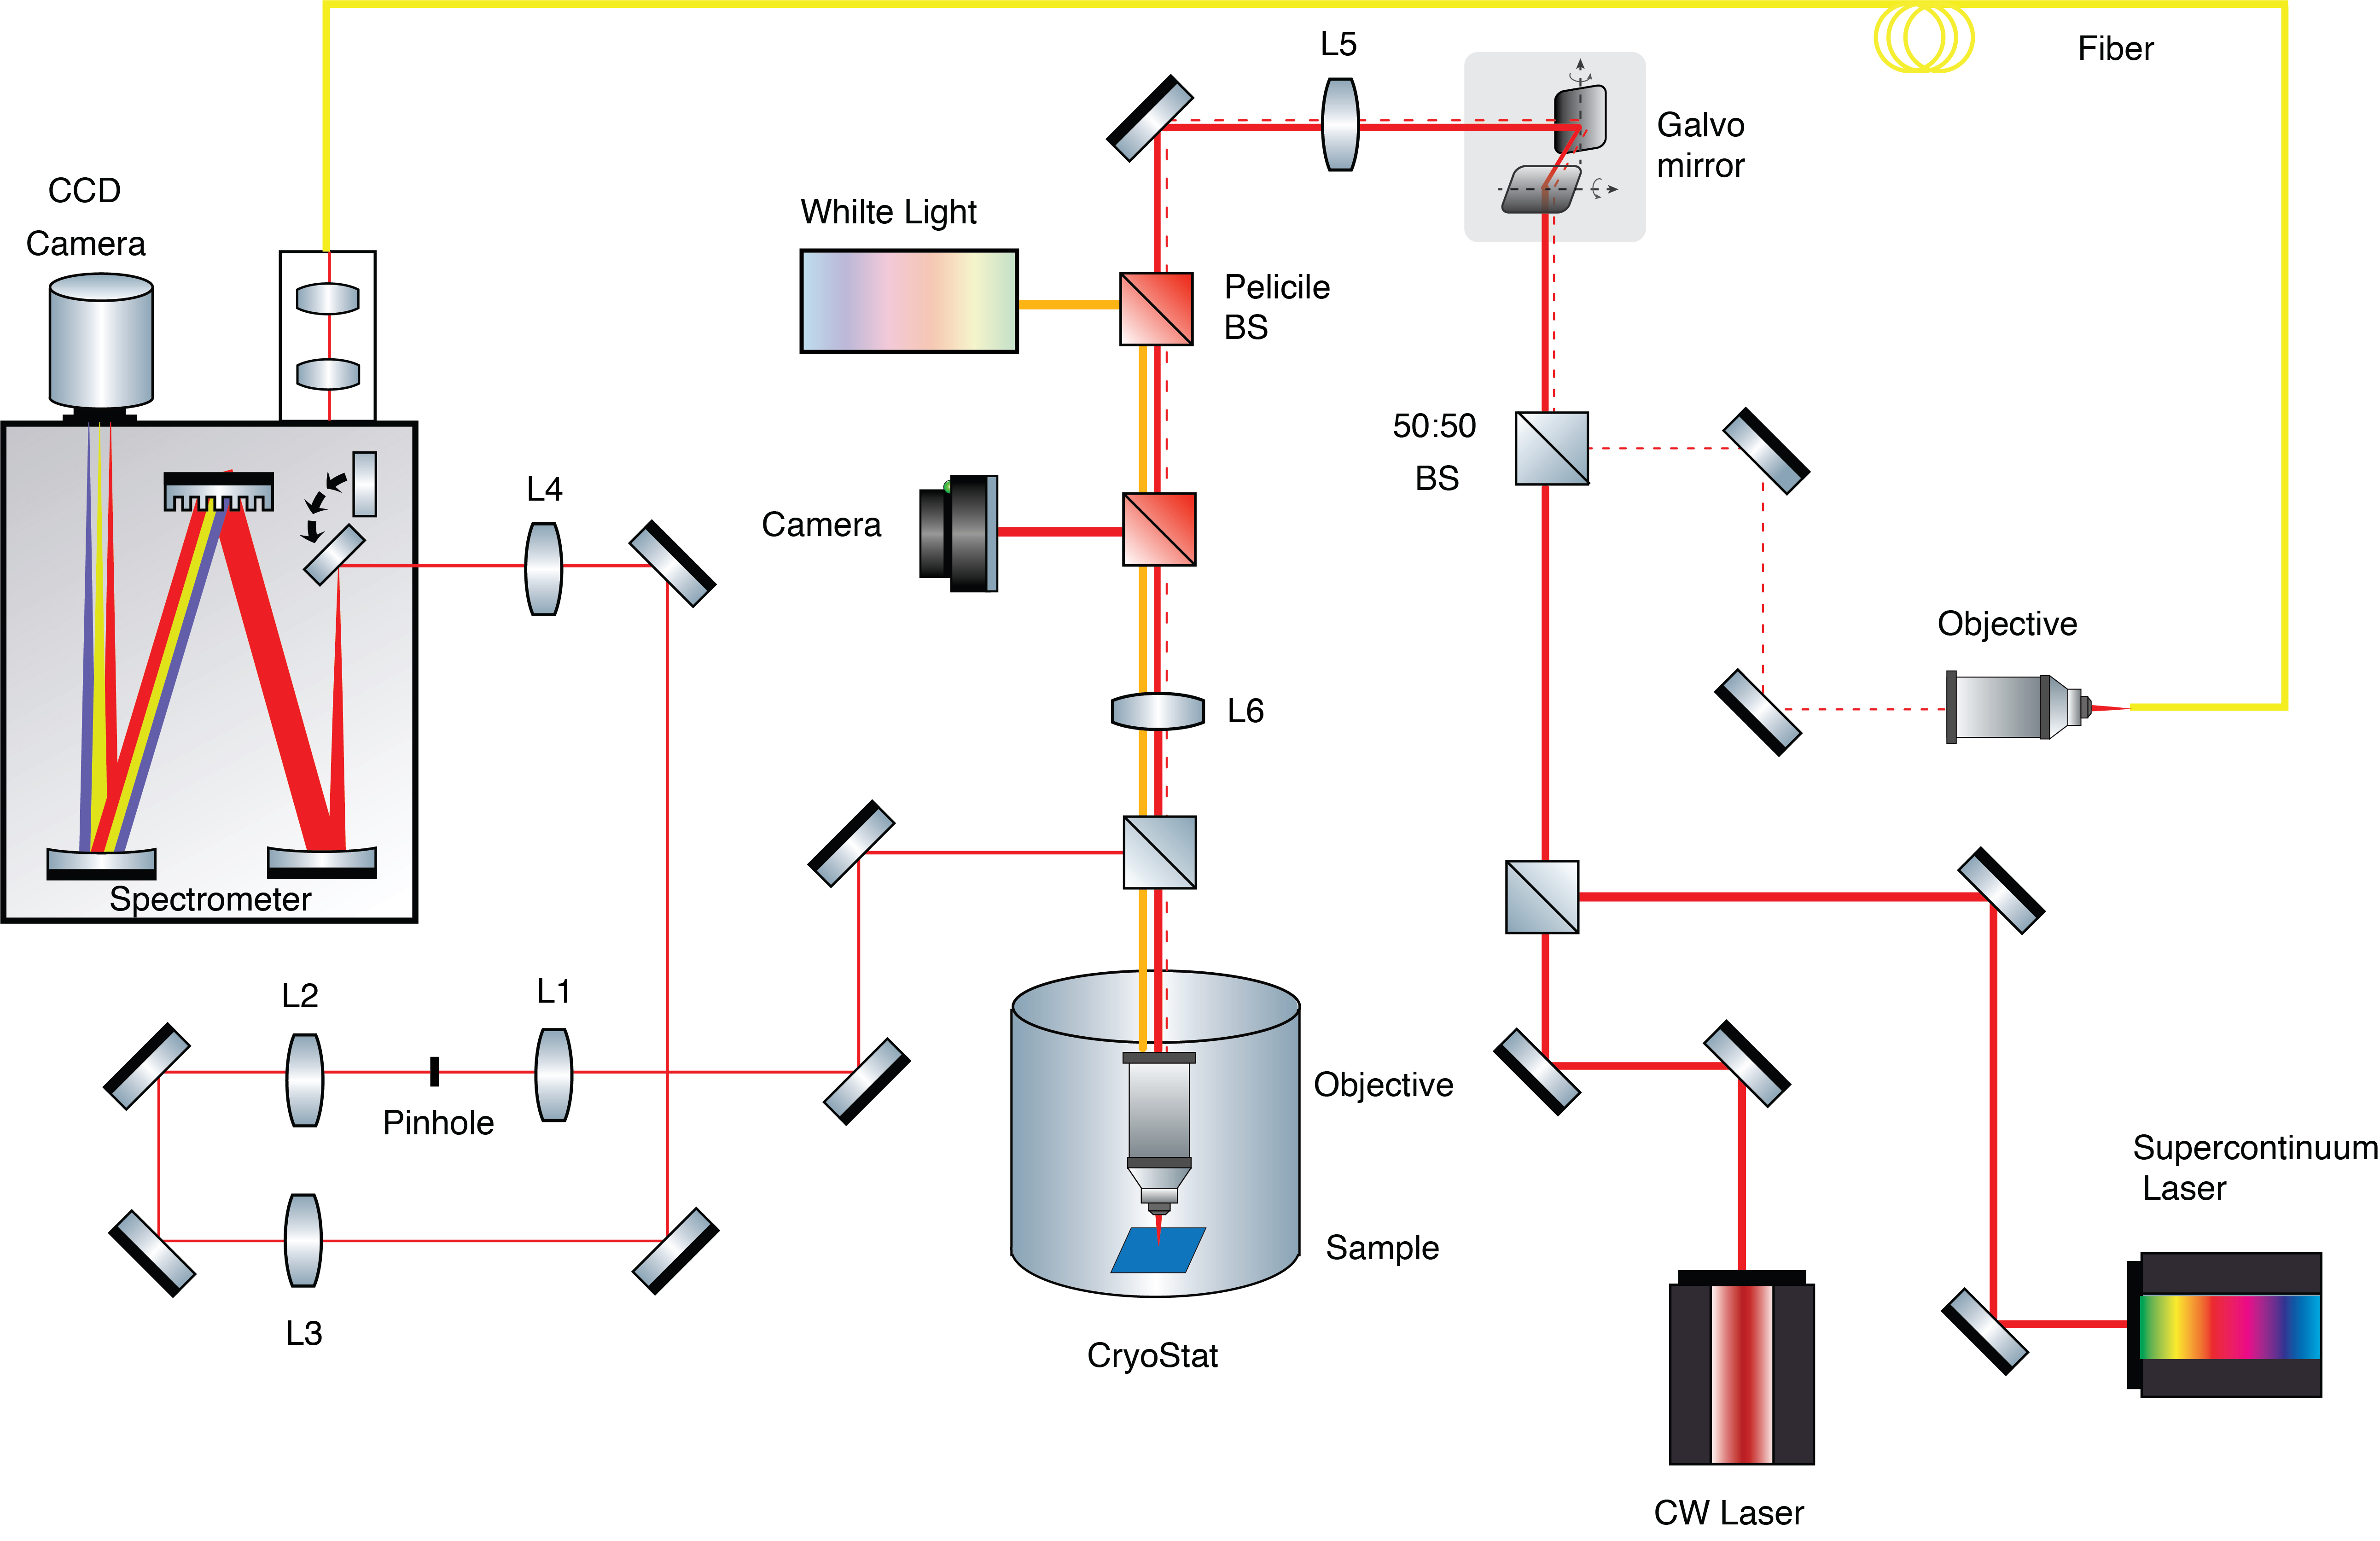
\includegraphics[width=1\textwidth]{Figures/C3/Fig.Setup.jpg} % 
\end{center}
\caption[Real-space and Fourier-space spectroscopy experimental setup.] {\textbf{Real-space and Fourier-space spectroscopy experimental setup.} L1 and L3(flip) are the Fourier plane relay lens. The distance before L1 to the objective is set as $2f_1$.  The distance between L1 and L3 is set as $2f_1+f_3$. L1 and L2(flip) are the real plane relay lens.The distance between L1 and L2 is set as $2f_1+f_2$.The pinhole is set at center between L1 and L2. L4 is the imaging lens for the spectrometer.}
\label{fig.OS}
\end{figure}
\end{quote}
\renewcommand{\baselinestretch}{2}
\small\normalsize
% --------------
%Chapter 4

\renewcommand{\thechapter}{4}

\chapter{Exciton confinement in moiré electrostatic superlattice}
\label{chap4}

Quantum confining excitons has been a persistent challenge in the pursuit of strong exciton interactions and quantum light generation. Unlike electrons, which can be readily controlled via electric fields, imposing strong nanoscale potentials on excitons to enable quantum confinement has proven challenging. 
In this study, we utilize piezoelectric force microscopy to image the domain structures of twisted hexagonal boron nitride (hBN), revealing evidence of strong 
in-plane electric fields at the domain boundaries. 
By placing a monolayer MoSe$_2$ only one to two nanometers away from the twisted hBN interface, we observe energy splitting of neutral excitons and Fermi polarons by several millielectronvolts at the moiré domain boundaries. 
By directly correlating local structural and optical properties, we attribute such observations to excitons confined in a nanoscale one-dimensional electrostatic potential created by the strong in-plane electric fields at the moiré domain boundaries.
Intriguingly, this 1D quantum confinement results in pronounced polarization anisotropy in the excitons’ reflection and emission, persistent to temperatures as high as ~80 Kelvins. 
These findings open new avenues for exploring and controlling strongly interacting excitons for classical and quantum optoelectronics.

\section{Introduction}

Quantum confinement of excitons enables fundamental studies of strongly interacting quantum many-body systems, such as strongly interaction excitons and quantum light generation \cite{Aharonovich2016-sl,Palacios-Berraquero2017-zr,Baek2020-qm,Hu2024-ua,Heithoff2024-jn,Shanks2021-qb,Thureja2022-cv} with applications to energy transfer and information processing\cite{Montblanch2023-ny,Butov2017-ls}. 
However, unlike electrons, which can be readily controlled via an electric field\cite{Wang2018-tm}, imposing strong nanoscale potential on excitons for quantum confinement has been challenging \cite{Butov2017-ls,Rapaport2005-fy}. Substantial progress has been made in confining excitons in van der Waals heterostructures based on atomically thin semiconductors\cite{Hu2024-ua,Heithoff2024-jn,Thureja2022-cv,Thureja2024-og}. 
Notably, nanoscale confinement of excitons has been achieved in the moiré patterns of two-dimensional semiconductors\cite{Jin2019-ce,Tran2019-uv,Wu2018-ty,Yu2017-so,Naik2022-qk,Seyler2019-ok}. This moiré potential, driven by interlayer electronic hybridization, can be remarkably strong, splitting the exciton energies by tens of meVs through quantum confinement\cite{Seyler2019-ok,Shabani2021-lf}. 
However, interlayer hybridization induces lattice relaxation and often a transition to an indirect band gap, causing undesirable effects such as exciton linewidth broadening and reduced quantum yield\cite{Tang2021-io,Huang2022-jh,Li2021-xh}. Alternatively, a recent approach uses the fringe in-plane electrical field of patterned gate electrodes to directly modulate the exciton energies without changing the materials’ band structures\cite{Heithoff2024-jn,Thureja2022-cv,Thureja2024-og}. Compared with moiré potential, the strength of the confinement is weaker, primarily limited by the gating geometry and electrical breakdown of dielectrics.


\section{Sample Fabrication}

Graphite, hBN flakes are mechanically exfoliated from the bulk crystals onto the silicon chip with SiO$_2$ layer. Exfoliated monolayer MoSe$_2$  flakes were provided by the Quantum Material Press (QPress) facility in the Center for Functional Nanomaterials (CFN) at Brookhaven National Laboratory (BNL). The thickness of the gated hBN flakes and MoSe$_2$ layer numbers are estimated based on the color contrast under optical microscopy. Twisted hBN flake thickness is identified by contact-mode AFM. The heterostructure is assembled in a transfer station built by Everbeing Int’l Corp., which uses PDMS (Polydimethylsiloxane) and PC (Polycarbonate) as stamp and transfer all the flakes in a dry transfer method onto a silicon chip with 285nm SiO$_2$ layer. Then the electrical contacts are patterned by electron-beam lithography and a liftoff process where we deposited 5nm of Cr and 80nm of Au by thermal evaporation.

\section{Results}
\subsection{In-plane polarization at the moiré domain boundaries revealed by PFM}

Here, we develop a method that takes advantage of both methods to realize strong confinement of excitons while maintaining the direct band gap. 
We leverage the recently discovered moiré ferroelectricity\cite{Woods2021-cn,Yasuda2021-is,Wang2022-hi,Kim2024-al} in twisted hexagonal boron nitride (hBN) to imprint a nanoscale potential on excitons in 2D semiconductors\cite{Gu2024-gk,Zhao2021-cm,Kim2025-jv}. 
Such imprinting of electrostatic potential modifies the electronic distribution inside the remote semiconducting layer, leading to the formation of charged excitons\cite{Cho2025-ai} and electronic Mott-Wigner states\cite{Kiper2025-ao}. 
Different from these earlier studies focusing on the effects of out-of-plane electric fields inside moiré domains\cite{Vizner-Stern2021-gx,Wu2021-cf}, we utilize the strong local in-plane electric fields at the moiré domain boundary (DB) to confine excitons within a narrow strip of $\sim$ ten nanometers. We further demonstrate that the same field leads to even stronger confinement of the Rydberg states due to their larger polarizability\cite{Heckotter2017-im}. 
These results open exciting avenues for studying many-body quantum systems, such as strongly interacting excitons and photons\cite{Froese2025-sz}, and novel ferroelectric control mechanisms for classical and quantum optoelectronics\cite{Zhang2024-mw,Sung2020-tn,Yang2024-er}. 

To create moiré superlattice domains, we stack two thin layers of hBN with a near $\sim 20^\circ$ target twist angle of\cite{Kim2024-al,Sung2020-tn}. The AB and BA stacking domains generate out-of-plane polarizations in opposite directions and an in-plane electric field near DBs (Figure~\ref{fig4.1} a). 
The in-plane field is predicted to be comparable to the out-of-plane polarization inside the domains\cite{Bennett2023-cs,Walet2021-zp}. 
Since the strength of the in-plane electric field decreases with increasing vertical distance \textit{d}\cite{Kim2024-al}, 
we select thin hBN layers ($\sim$ 2 nm) so the twisted interface remains close to the sample surface and characterize the surface with piezoelectric force microscopy (PFM). 
Unlike Kelvin probe force microscopy (KPFM), which is sensitive to surface potential arising from out-of-plane polarizations \cite{Woods2021-cn,Kim2024-al,Kim2025-jv,Vizner_Stern2021-ls,Han2024-bh,Weston2022-jl}, 
PFM detects both out-of-plane and in-plane polarizations from different modes of cantilever movements, such as vertical displacement, buckling, and torsion\cite{Li2024-un,Chiodini2025-qj}, distinguished by their respective photodiode responses\cite{McGilly2020-nz}(Figures ~\ref{fig4.1} b,c).

Here, we focus on the in-plane polarization at the twisted hBN DBs. 
Figures~\ref{fig4.1}d,e present the measured PFM amplitude and phase maps, revealing the clear formation of multiple domains, even though no obvious features are observed in the corresponding topography map(Figure~\ref{fig4.1s}b). 
Domain sizes vary significantly across different regions, ranging from a few tens of nanometers to several micrometers, due to local variations in the twist angle. 
Interestingly, we observe the strongest piezoelectric response at the domain boundaries with weaker contrast across the two types of domains, in contrast to KPFM of similar systems\cite{Woods2021-cn,Vizner-Stern2021-gx}.
Furthermore, the PFM response at DBs is most pronounced when the boundary aligns parallel to the cantilever and changes its sign depending on boundary orientations.

These observations reveal a strong in-plane electric field at the DBs. 
As shown in Figures~\ref{fig4.1}b,c, when DBs is parallel to the cantilever, the in-plane polarization perpendicular to the boundary induces torsion of the cantilever, generating a PFM signal. 
The sign of the PFM signal at DBs therefore reflects the different directions of the in-plane electric field. 
When the in-plane field is parallel to the cantilever, the cantilever buckles, which is detectable via vertical motion and has been recently reported\cite{Chiodini2025-qj,Wan2024-wj}.
However, in our experiments, this corresponding vertical signal is not selected by the photodiode, further evidenced by the uniform amplitude across different domains. 

%%///////////////Figure panel///////////////////////////
%Fig.1--------------
\renewcommand{\baselinestretch}{1}
\small\normalsize
\begin{quote}
\begin{figure}
\begin{center}
% \includegraphics[0in,0in][3.25in,4.266in]{nlsetime.eps}
\includegraphics[width=0.9\textwidth]{Figures/C4/figure1-4.jpg} % 
\end{center}
\caption[caption] {\textbf{In-plane electric field in twisted hBN triangular Moiré superlattice.} \textbf{a,} Top and side views of the in-plane electric field at domain boundaries (DBs) in twisted hBN moiré superlattice. The surface potential difference across the domains creates an in-plane electric field, which decays with increasing vertical distance from the interface. \textbf{b, c,} Different modes of PFM cantilever displacement in response to the in-plane electric field and corresponding photodiode responses. \textbf{d, e,} PFM amplitude and phase map of a twisted hBN sample showing varying domain size.}
\label{fig4.1}
\end{figure}
\end{quote}
\renewcommand{\baselinestretch}{2}
\small\normalsize
% --------------

%Fig.2--------------
\renewcommand{\baselinestretch}{1}
\small\normalsize
\begin{quote}
\begin{figure}
\begin{center}
\includegraphics[width=0.8\textwidth]{Figures/C4/figure-S1-3.jpg} % 
\end{center}
\caption[Optical image and PFM map of Device D1] {\textbf{Optical image and PFM map of Device D1.} \textbf{a,} Optical image of the R-stacked twisted hBN.\textbf{b,}Topography and \textbf{c,} PFM amplitude image of the region indicated by the purple box in \textbf{a}. After PFM characterization, we stack the monolayer MoSe2 on top of the twisted hBN surface and then encapsulate it with gate hBN and top graphite. \textbf{d,}The optical image and \textbf{e,} the device schematic of the final device.}
\label{fig4.1s}
\end{figure}
\end{quote}
\renewcommand{\baselinestretch}{2}
\small\normalsize
% --------------
%%///////////////Figure panel End///////////////////////////

\subsection{Confining excitons by in-plane electric field}

Next, we integrate a monolayer MoSe$_2$ flake on top of the twisted hBN and encapsulate it with additional top hBN and graphene. The entire fabrication process was performed without heating the samples to a high temperature to avoid perturbation of the domain structures. We then perform the reflectance and PL measurements of the sample at 5 K to establish a correlation between the twisted hBN domain sizes and the MoSe$_2$ exciton spectroscopic features.

We first characterize excitons in regions with large domains of $\sim$ 1-2 µm shown in Figure~\ref{fig4.2} a, where a single domain can be resolved in the far field.
Figures~\ref{fig4.2} b,c show the corresponding reflectance spectrum of the MoSe$_2$ taken within the region. 
However,when the laser is within a single domain, both PL and reflection spectra show a single exciton peak, similar to MoSe$_2$ encapsulated in non-twisted hBN\cite{Scuri2018-bn}. 
However, when the laser moves on to the domain boundaries, we observe a split in the exciton energy of around $\sim$ 3 meV in both PL and reflectance, dramatically different from typical hBN-encapsulated monolayers.

We further investigate how the energy splitting varies as a function of domain size across the sample. 
As shown in Figures~\ref{fig4.2} d,e, we observe that exciton energy splitting increases as domain size decreases, reaching as high as $\sim$ 7 meV when the domain size is approximately 250 nm.
Since these domain sizes are below the diffraction limit, the measured exciton response includes contributions from both within the domains and along the domain walls.
Interestingly, the exciton splitting also correlates with the strength of the in-plane electric field. 
By comparing regions with similar domain sizes but different in-plane electric fields, as indicated by PFM amplitude, we observe larger exciton splitting in areas with stronger in-plane fields (see difference in Figure~\ref{fig4.3} d,e).

Several mechanisms can influence the excitonic spectra of MoSe$_2$ on twisted hBN. 
For instance, out-of-plane polarization can introduce varying doping levels across different domains\cite{Cho2025-ai,Choi2024-ei,Soubelet2021-hc}. 
While this may shift the exciton energy, a pure doping effect would not cause exciton splitting, since the doping—and thus the exciton resonance—are expected to change continuously across domains\cite{Cho2025-ai}. 
In contrast, inhomogeneous strain can shift and split exciton energy\cite{Mitioglu2018-qt,Glazov2022-vs}. 
This effect can occur even in TMDs encapsulated in non-twisted hBN, often arising uncontrollably in areas with strong strain gradients, such as near bubbles\cite{Darlington2020-ok}.

Another possible mechanism is related to the in-plane electric field $F_x$ at the domain boundaries. 
In particular, modifies the exciton energy by:
\begin{equation}
\Delta E = -\frac{1}{2}\,\alpha \lvert F_x \rvert^2
\label{eq:stark}
\end{equation} 
where $\alpha$ is the polarization coefficient of excitons\cite{Thureja2022-cv,Pedersen2016-pv}. 
Therefore, a strong and spatially localized $F_x$ at the moiré domain boundaries can create a nanoscale confinement potential $V_x$ for excitons, which induces exciton energy splitting \cite{Hu2024-ua,Heithoff2024-jn,Thureja2022-cv,Thureja2024-og} (Figure~\ref{fig4.2}f). 
Observing exciton splitting exclusively near domain boundaries in large-domain regions suggests that this electrostatic effect may play a significant role in our studies. 
This also explains the larger exciton splitting observed at regions with stronger PFM response and smaller domains, where smaller domains likely correspond to narrower domain walls and tighter confinement.

%%///////////////Figure panel En///////////////////////////
%Fig.3--------------
\renewcommand{\baselinestretch}{1}
\small\normalsize
\begin{quote}
\begin{figure}
\begin{center}
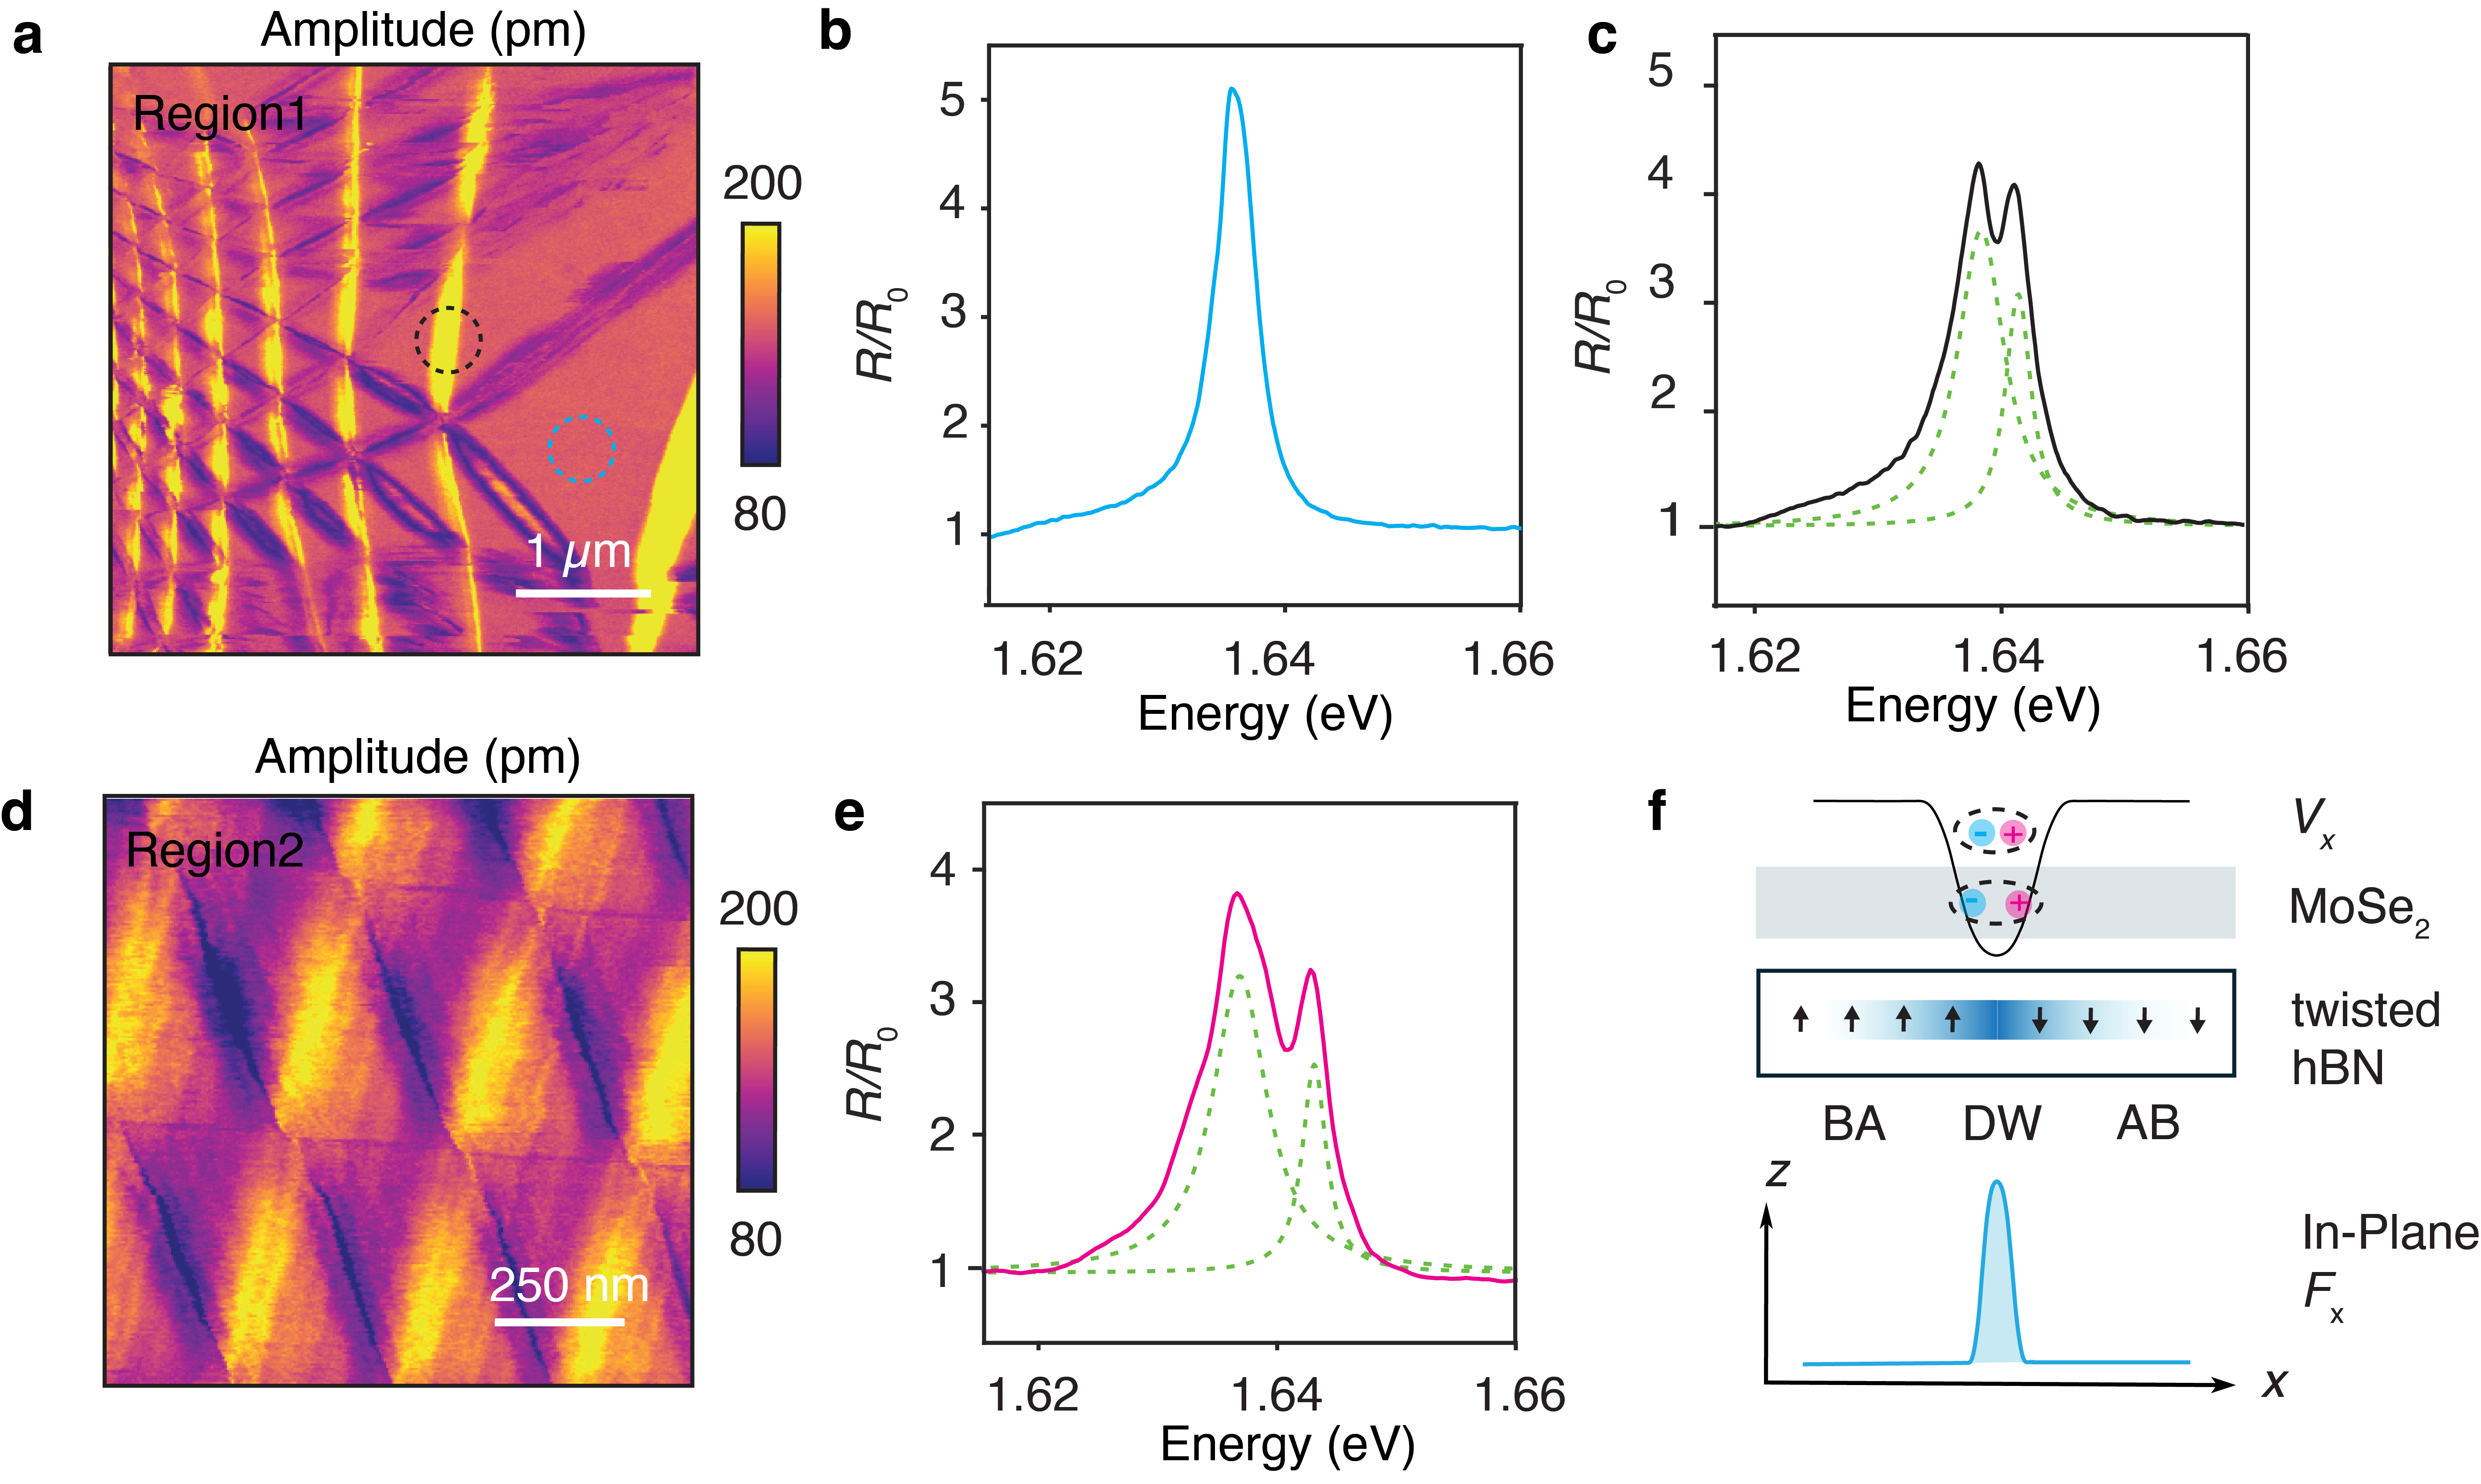
\includegraphics[width=1\textwidth]{Figures/C4/figure2-2.jpg} % 
\end{center}
\caption[caption] {\textbf{Confined intralayer excitons by the in-plane electric field.} \textbf{a,} PFM image of the electrostatic superlattice showing different sizes of triangular domains.\textbf{b,} Normalized reflectance taken at the large domain area indicated as the blue spot in \textbf{a}. \textbf{c,} Normalized reflectance taken at the domain boundary indicated as the black spot in \textbf{a}. Green dashed lines are Lorentzian fit, and the solid line is measured data. \textbf{d,} PFM image of a region with sub-diffraction-limit domains. \textbf{e,} Normalized reflectance spectra taken at the region in \textbf{d}. \textbf{f,} Schematic of the field-induced confinement potential $V_x$ confining intralayer excitons in MoSe$_2$ adjacent to the twisted hBN at the domain boundary.}
\label{fig4.2}
\end{figure}
\end{quote}
\renewcommand{\baselinestretch}{2}
\small\normalsize
% --------------
%%///////////////Figure panel End///////////////////////////

\subsection{1D Confinement nature of excitons}

Excitons confined in 1D potential, such as along moiré domain walls, are expected to exhibit strong anisotropic optical properties\cite{Thureja2022-cv,Bai2020-ih} (Figure~\ref{fig4.3} a). 
Therefore, to test our hypothesis further, we measure how reflectance and PL spectra of the excitons vary as a function of the linear polarization angle. 
First, we study the region with large domains so that only a single domain boundary contributes to the optical signal in the far-field (Figures~\ref{fig4.3} b,c). 
As shown in Figures~\ref{fig4.3} d-f, we observe anisotropic exciton reflection and emission with high degrees of linear polarization. 
By mapping the polarizer direction to the real-space angles on the sample, we find that the exciton polarization directions are parallel to the domain boundaries and remain so across the sample. 
As shown in Figures~\ref{fig4.3} d,e, when the domain wall orientations rotate by $20^\circ$ across two regions, we observe a similar amount of rotation in the linear polarization axis of the excitons. 
In contrast, we did not observe any polarization-dependent behaviors in regions with a single exciton resonance without splitting (Figure~\ref{fig.s2} e). 
Similar exciton splitting and linear polarization behaviors are also observed in more than four different samples with similar structures. 

The observed polarization dependence can be attributed to the 1D confinement at the domain boundary. 
In monolayer TMDs, due to electron-hole exchange interactions, the exciton dispersion splits into longitudinal and transverse branches, which have a coherent superposition of K and -K valley excitons at zero momentum\cite{Yu2014-gi}.
A 1D confinement potential breaks the $C_3$ in-plane rotation symmetry and splits the longitude and transverse branch at the zero momentum, which couples to light in two orthogonal directions \cite{Glazov2015-us,Yu2015-br,Qiu2015-vl} (Figure~\ref{fig.4.3} a).
With sufficiently strong confinement, this x–y polarization energy splitting surpasses the confinement energy, resulting in all confined modes becoming linearly polarized, as observed in our experiments. 
This linear polarization in reflection and emission also strongly suggests that inhomogeneous strain is not the dominant factor here. 
In control experiments observing exciton splitting on non-twisted hBN substrates, the two strain-split exciton resonances have random polarization angle dependence, likely due to variations of the local strain (Fig.~\ref{fig.s3}). 

Furthermore, remarkbly, we find that the 2s exciton state exhibits a larger energy splitting than the 1s state (Figure~\ref{fig.s7}), consistent with its greater polarizability. 
This further supports our conclusion that the splitting is not caused by strain, which would shift the 1s and 2s states by a similar amount.

Consistent with the quantum confinement picture, we find that the lower-energy peak is constantly redshifted relative to the free excitons. 
The higher-energy peak, however, appears near the free exciton energy due to overlapping contributions from both confined and bulk excitons—an effect of our optical probe being much larger than the domain walls.
Additional evidence of exciton confinement comes from power-dependent PL measurements. 
Compared to free 2D excitons, the 1D confined excitons exhibit significantly faster saturation (Figure~\ref{fig.s6}), consistent with the expectation of enhanced exciton–exciton interactions within the confined systems.

Further evidence can also be found in regions where the domain size falls below the diffraction limit. 
In these regions, the exciton reflectance and emission are no longer linearly polarized but still exhibit an anisotropic response. 
Notably, in specific spots, two local maxima of PL emission are observed at polarization angles separated by roughly sixty degrees (Figure.~\ref{fig.s2} d). 
These phenomena can be understood from the non-perfect triangle shapes of domain boundaries measured from PFM, where one particular domain wall direction would contribute more to the measured optical signal than the other directions.

%///////////////////////Figure Panel/////////////////////////

%Fig.4--------------
\renewcommand{\baselinestretch}{1}
\small\normalsize
\begin{quote}
\begin{figure}
\begin{center}
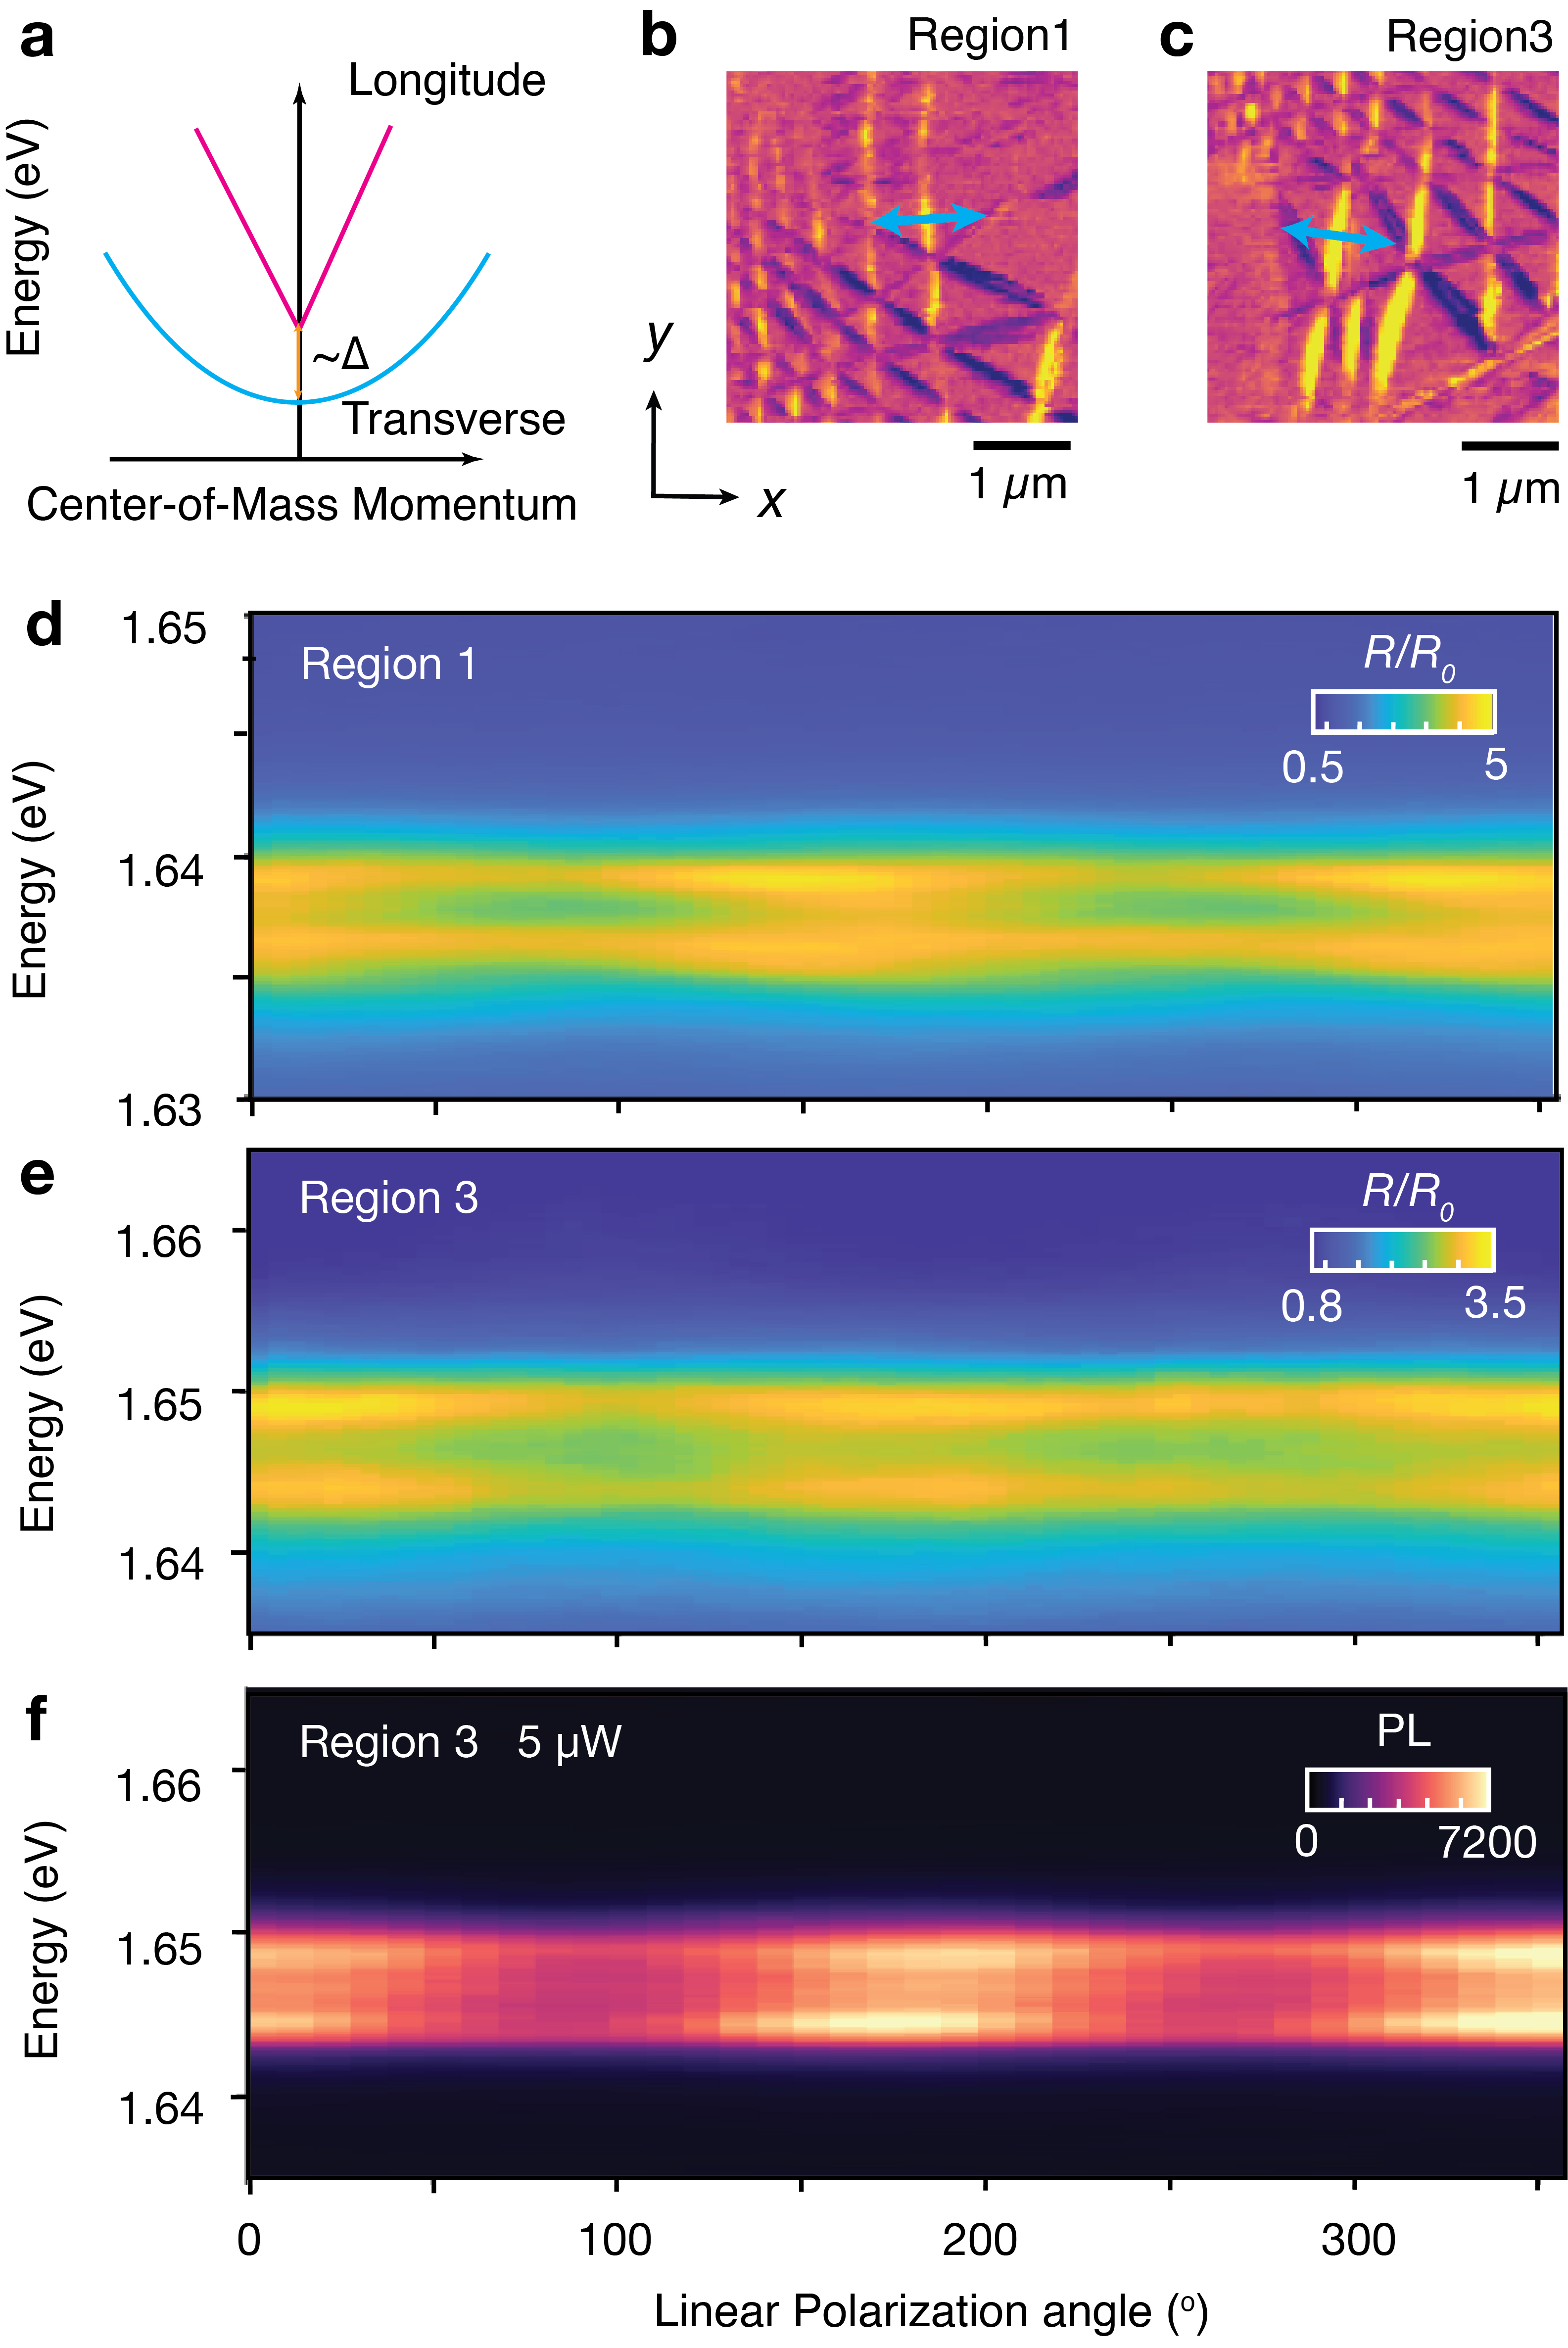
\includegraphics[width=0.7\textwidth]{Figures/C4/figure3-7.jpg} % 
\end{center}
\caption[caption] {\textbf{1D confinement at the domain boundary.} \textbf{a,} Schematic of the confined exciton dispersion. Under spatial localization, the exciton longitude and transverse branch become split with a magnitude of $\sim\Delta$ at zero center-of-mass momentum.\textbf{b,c,} PFM map of \textbf{b,} regions 1 and \textbf{c,} regions 3. \textbf{d,e,} Normalized reflectance as a function of the excitation linear polarization angle in regions 1 and 3 as indicated by the blue arrow in \textbf{b} and \textbf{c}, respectively. \textbf{f,} PL emission as a function of linear polarization with $5\,\mu\mathrm{W}$ excitation power from $635\,\mathrm{nm}$ CW laser. The spot is the same one taken in \textbf{e}.}
\label{fig4.3}
\end{figure}
\end{quote}
\renewcommand{\baselinestretch}{2}
\small\normalsize
% --------------

%Fig.5--------------
\renewcommand{\baselinestretch}{1}
\small\normalsize
\begin{quote}
\begin{figure}
\begin{center}
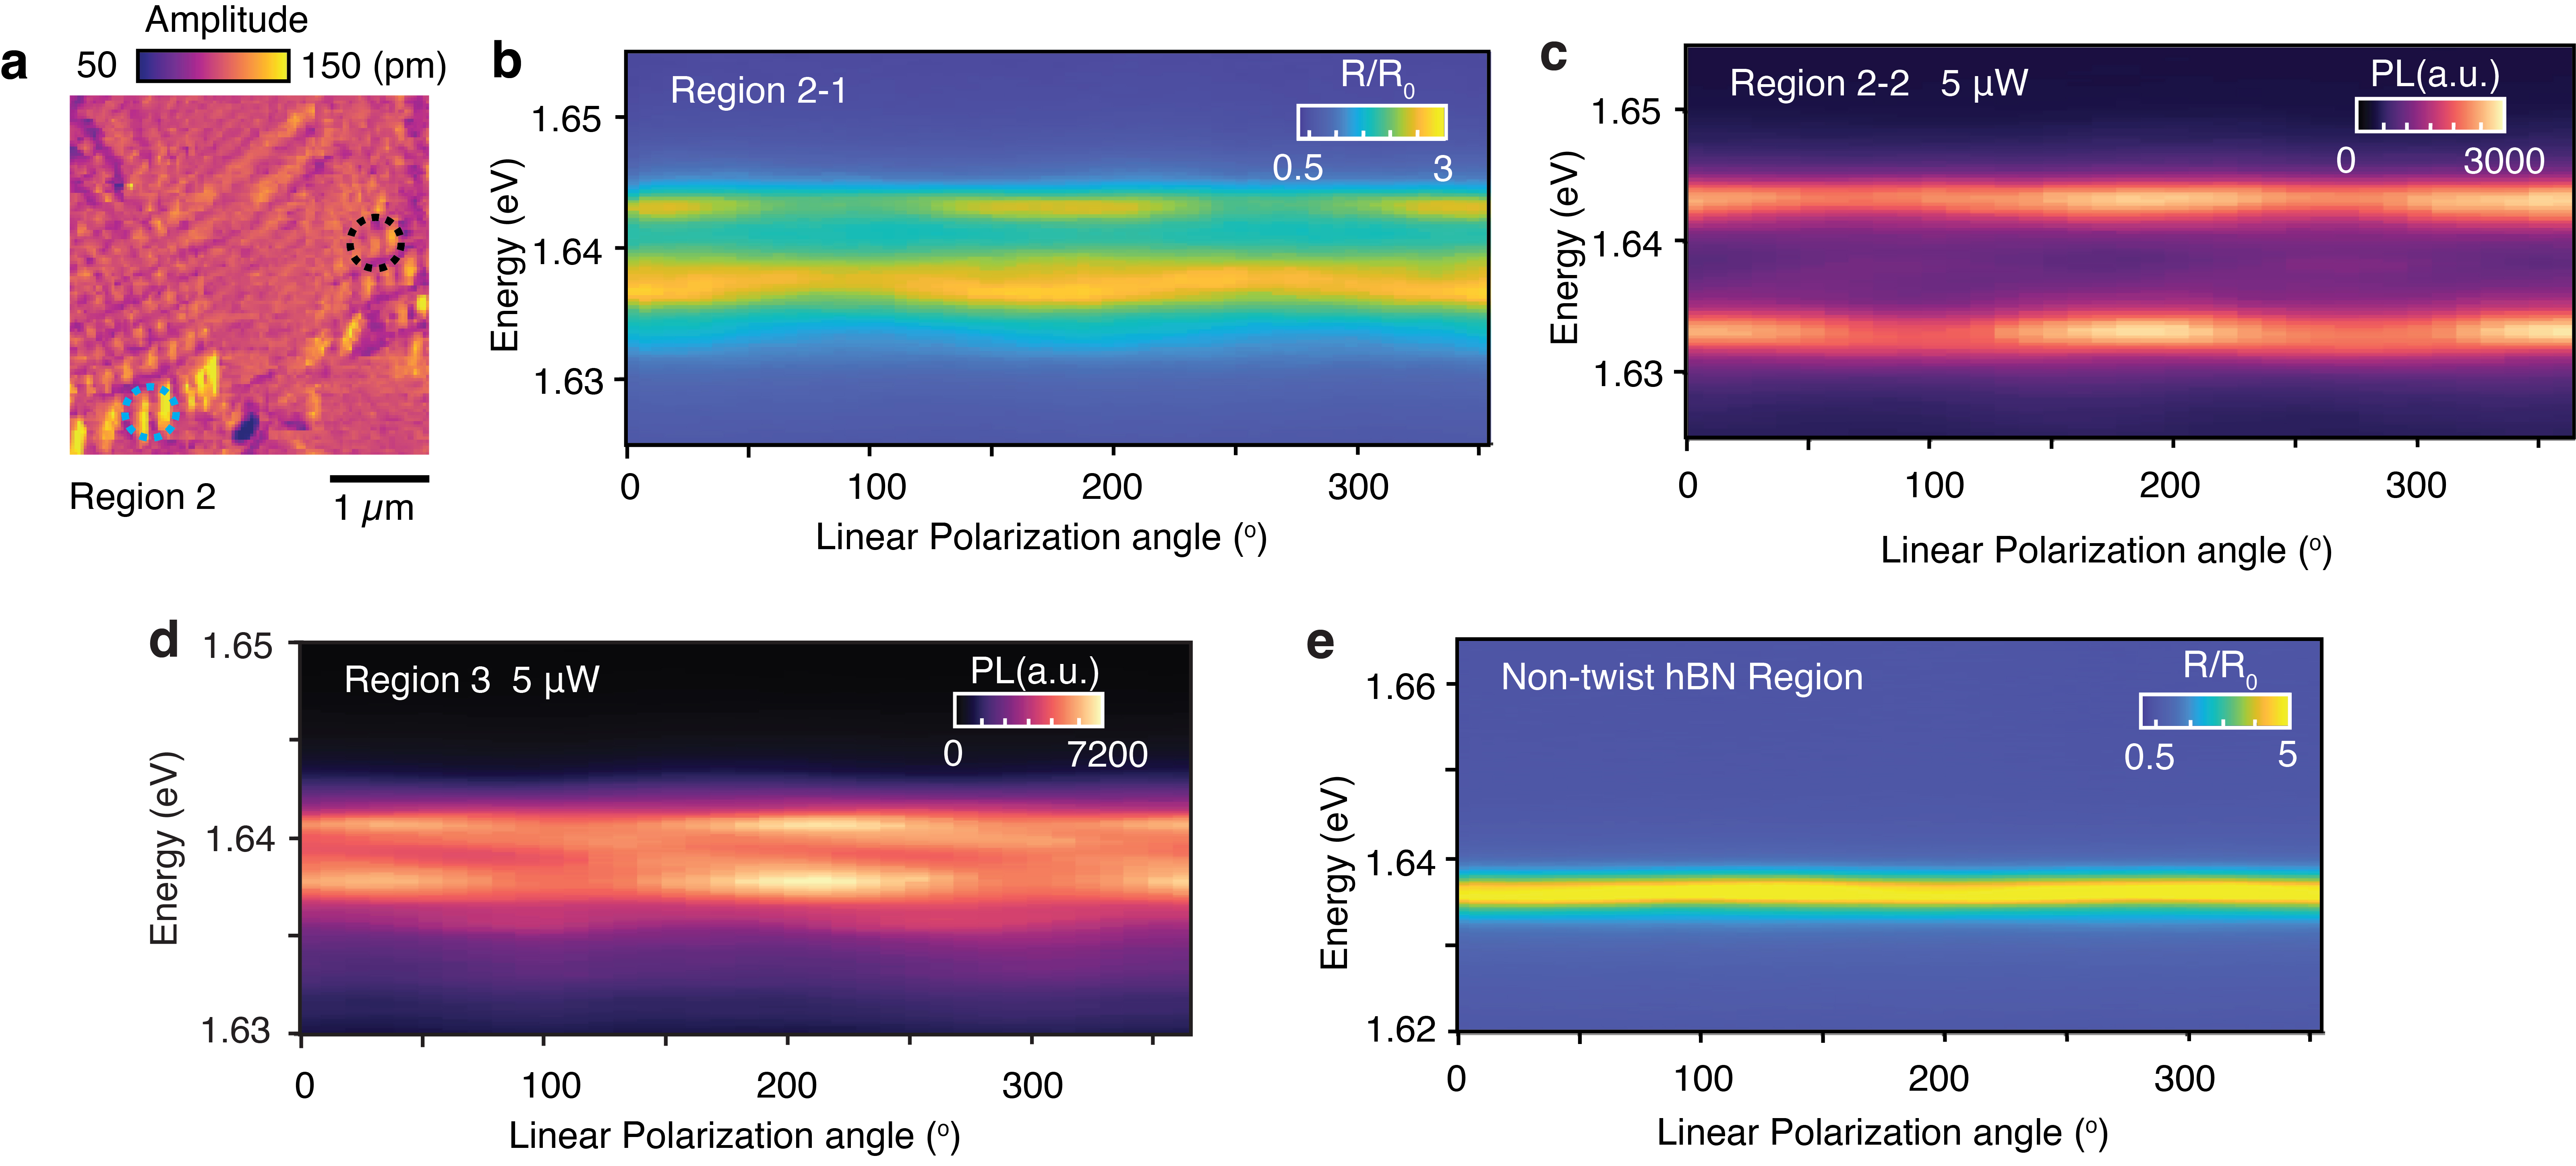
\includegraphics[width=1\textwidth]{Figures/C4/figure-S2.jpg} % 
\end{center}
\caption[caption] {\textbf{Polarization dependence of excitons in regions with sub-diffraction domains.} \textbf{a,} PFM amplitude map of region 2. The blue and black dashed circles correspond to the detection spot in \textbf{b} and \textbf{c}, respectively. 
\textbf{b,} Linear polarization dependence of the exciton reflection in region 2-1. \textbf{c,} Linear polarization dependence of PL in regions 2-2, which has a small domain size below the diffraction limit (smaller than 200 nm). The splitting energy of the two resonances is around 10 meV. \textbf{d,} Linear polarization PL emission for the similar spot in Fig.~\ref{fig4.3} b (region 2). As the laser spot detects two domains simultaneously, there are two maxima in the PL polarization angle, which are separated by a nearly $60^\circ$. This can be understood from the non-perfect triangle shapes of domain boundaries measured from PFM, where one particular domain wall direction would contribute more to the measured optical signal than the other directions. \textbf{e,} Linear polarization dependence of the reflectance taken at the non-twist hBN region. No obvious polarization dependence is observed. }
\label{fig.s2}
\end{figure}
\end{quote}
\renewcommand{\baselinestretch}{2}
\small\normalsize
% --------------

%Fig.6--------------
\renewcommand{\baselinestretch}{1}
\small\normalsize
\begin{quote}
\begin{figure}
\begin{center}
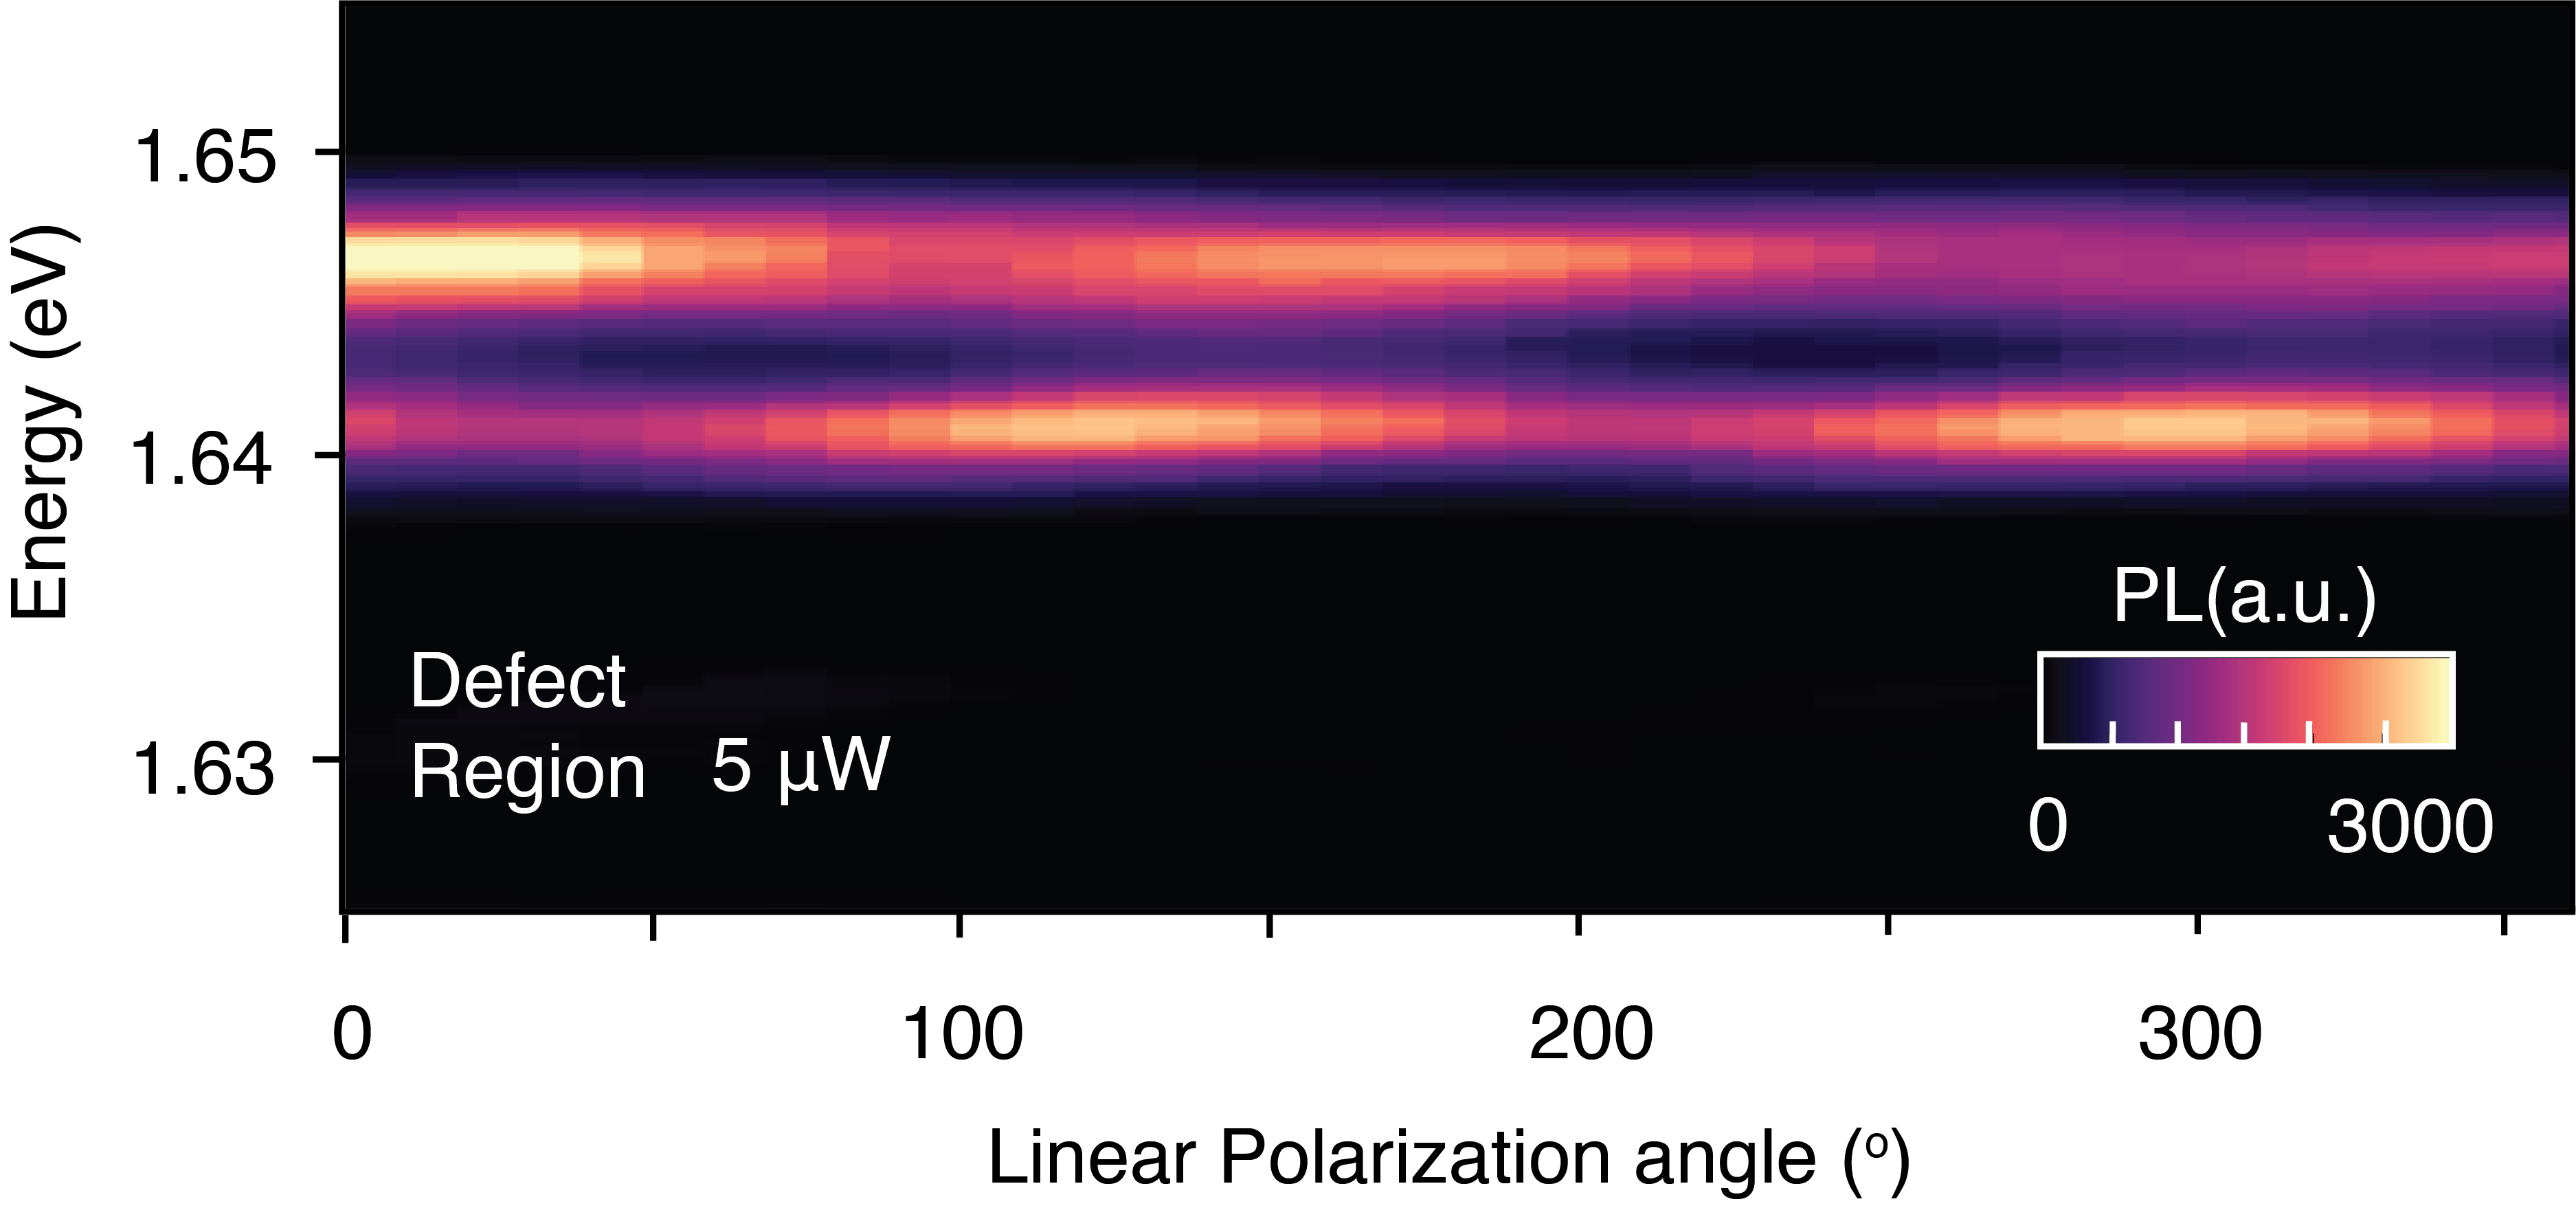
\includegraphics[width=0.7\textwidth]{Figures/C4/figure-S3.jpg} % 
\end{center}
\caption[caption] {\textbf{Polarization dependence of energy-split excitons caused by strain} In regions where local strain splits the exciton peaks, the two exciton peaks do not have the same linear polarization.}
\label{fig.s3}
\end{figure}
\end{quote}
\renewcommand{\baselinestretch}{2}
\small\normalsize
% --------------

%Fig.7--------------
\renewcommand{\baselinestretch}{1}
\small\normalsize
\begin{quote}
\begin{figure}
\begin{center}
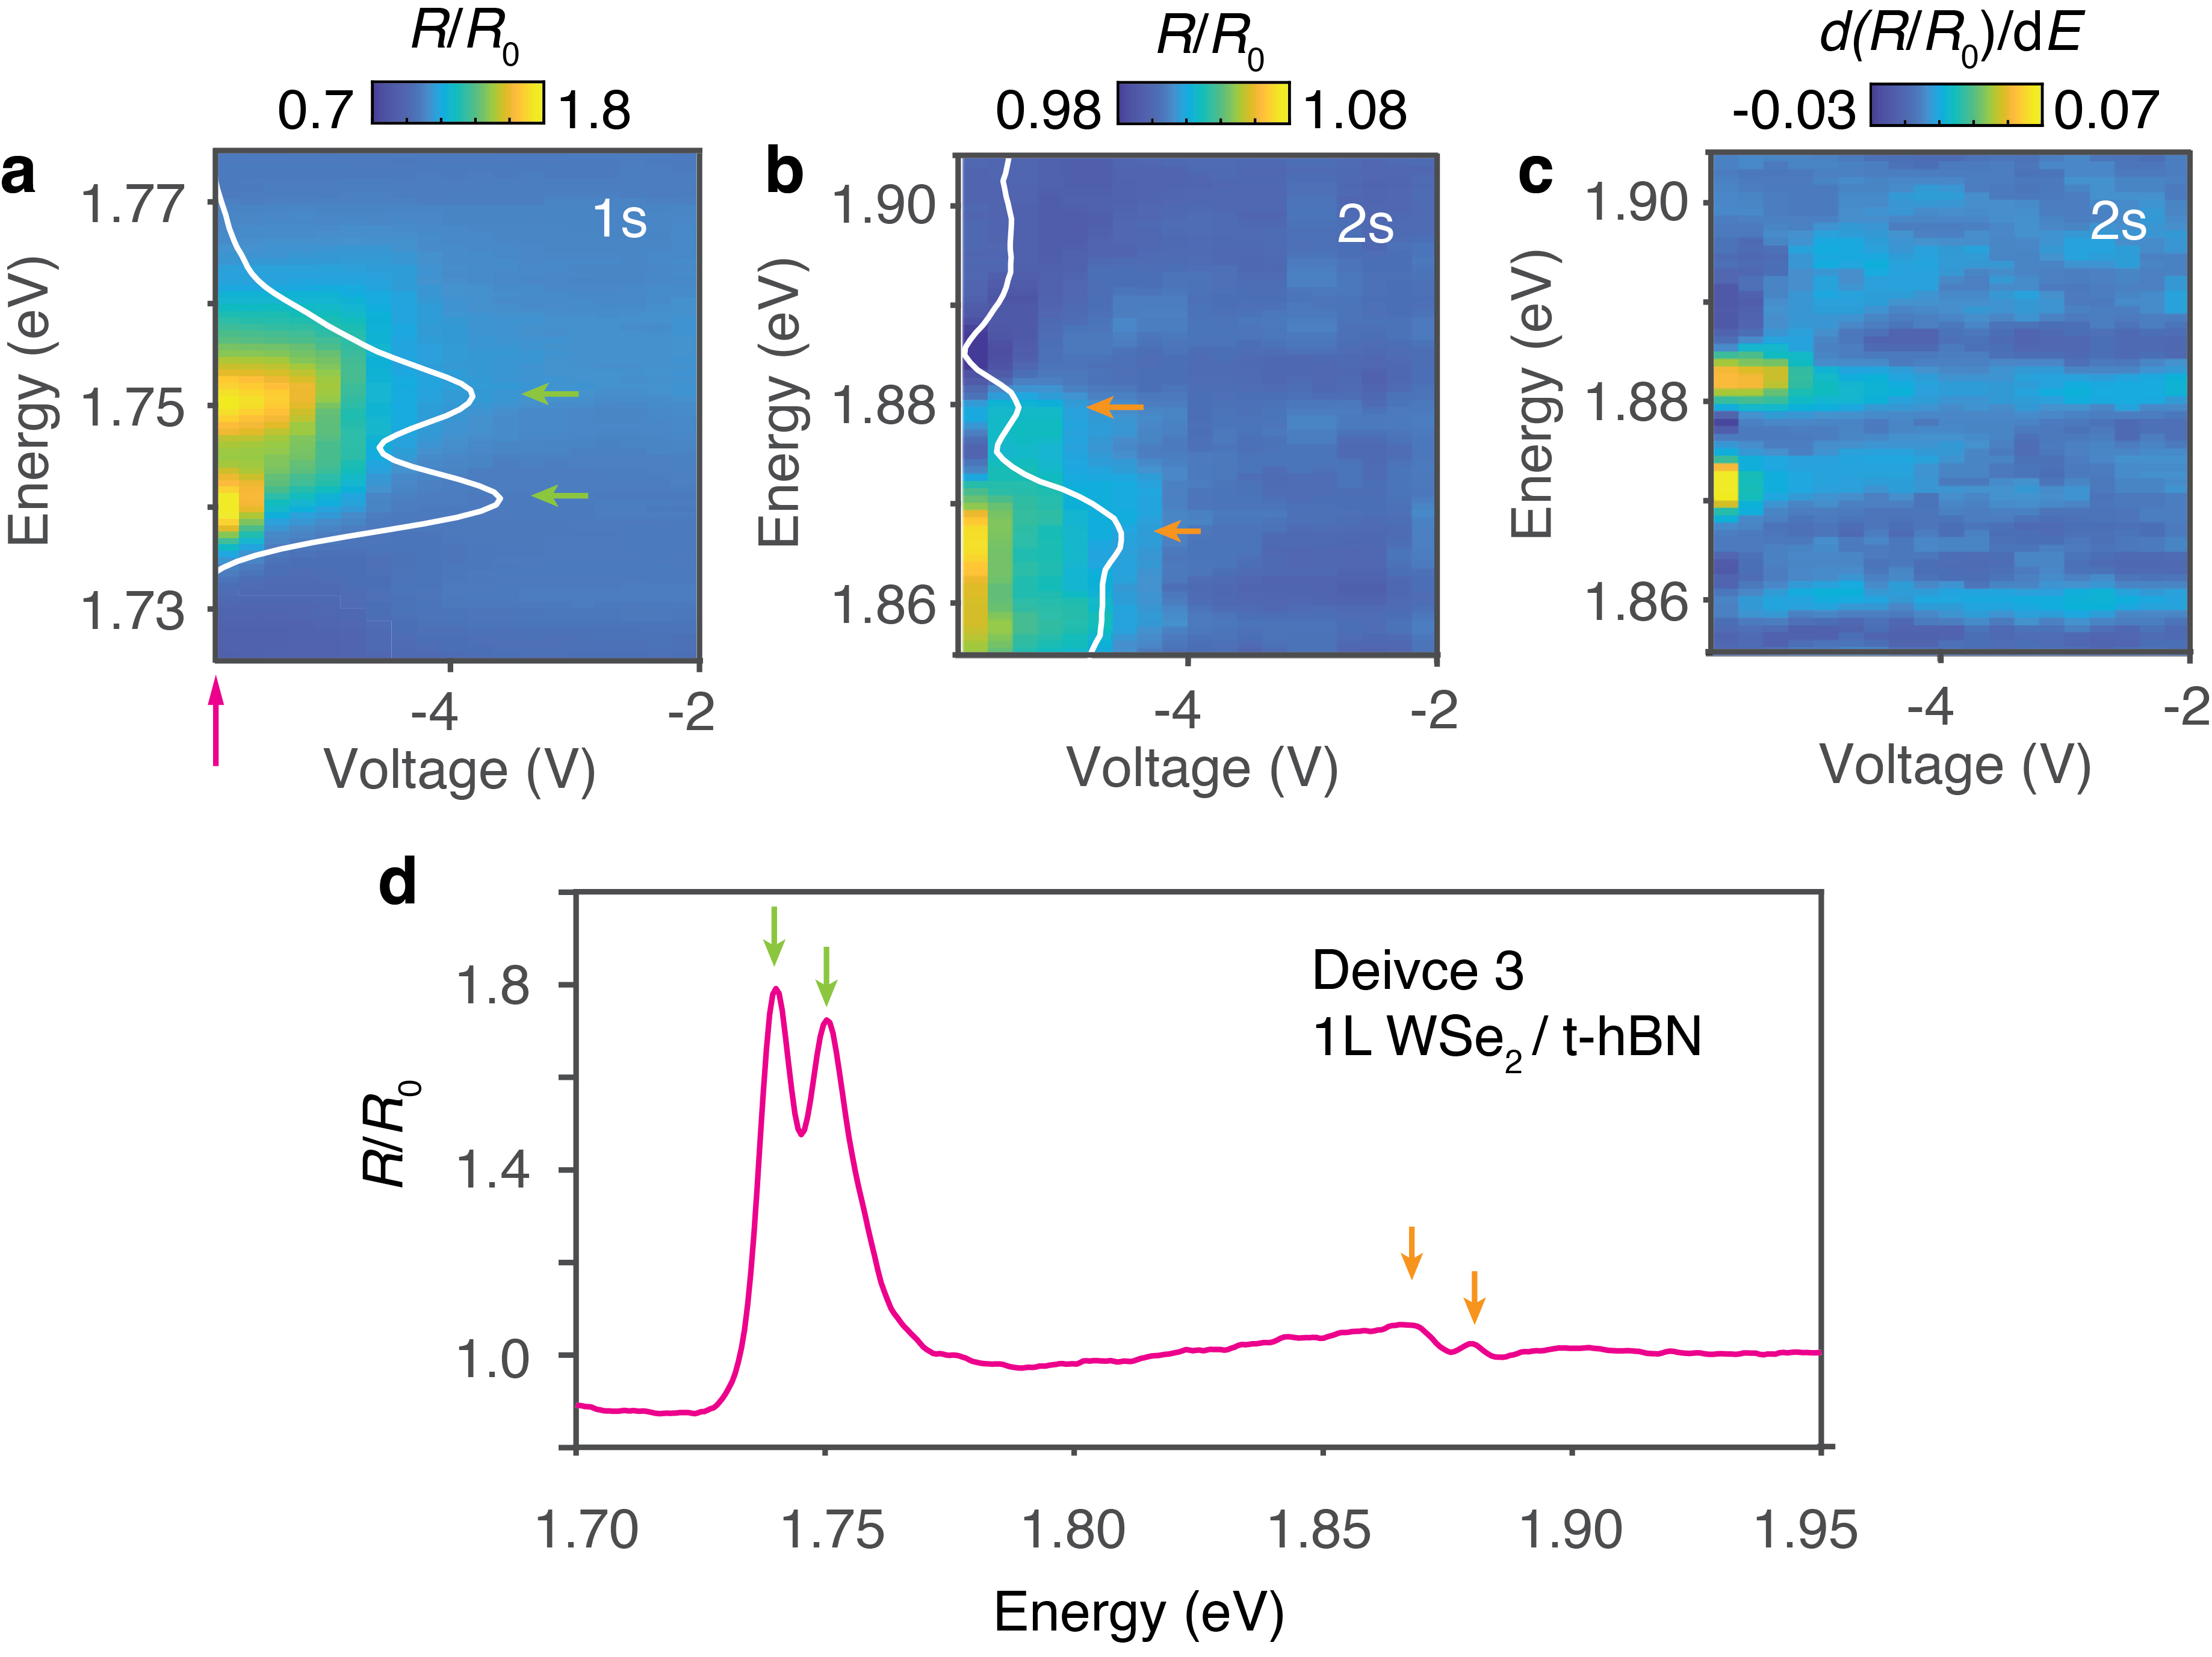
\includegraphics[width=0.8\textwidth]{Figures/C4/figure-S7.jpg} % 
\end{center}
\caption[Rydberg exciton] {\textbf{Quantum confinement of 2S exciton in 1L $WSe_2$ / twisted hBN.} \textbf{a,} 1s exciton and \textbf{b,} 2s exciton splitting shown in normalized reflectance. \textbf{c,} Normalized reflectance spectrum at charge neutral point. The energy splitting is $\sim$ 10 meV for 1s exciton and $\sim$ 13 meV for 2s exciton. For monolayer $WSe_2$ on the same twisted hBN interface, a larger energy splitting than that of MoSe$_2$ is expected due to a larger polarizability of $\alpha \sim 10.2~\text{eV}\,\text{nm}^2/\text{V}^2$ in $WSe_2$ for 1s exciton. The 2s exciton owns even larger splitting due to its large Bohr radius and thus larger polarizability.}
\label{fig.s7}
\end{figure}
\end{quote}
\renewcommand{\baselinestretch}{2}
\small\normalsize
% --------------


%Fig.8--------------
\renewcommand{\baselinestretch}{1}
\small\normalsize
\begin{quote}
\begin{figure}
\begin{center}
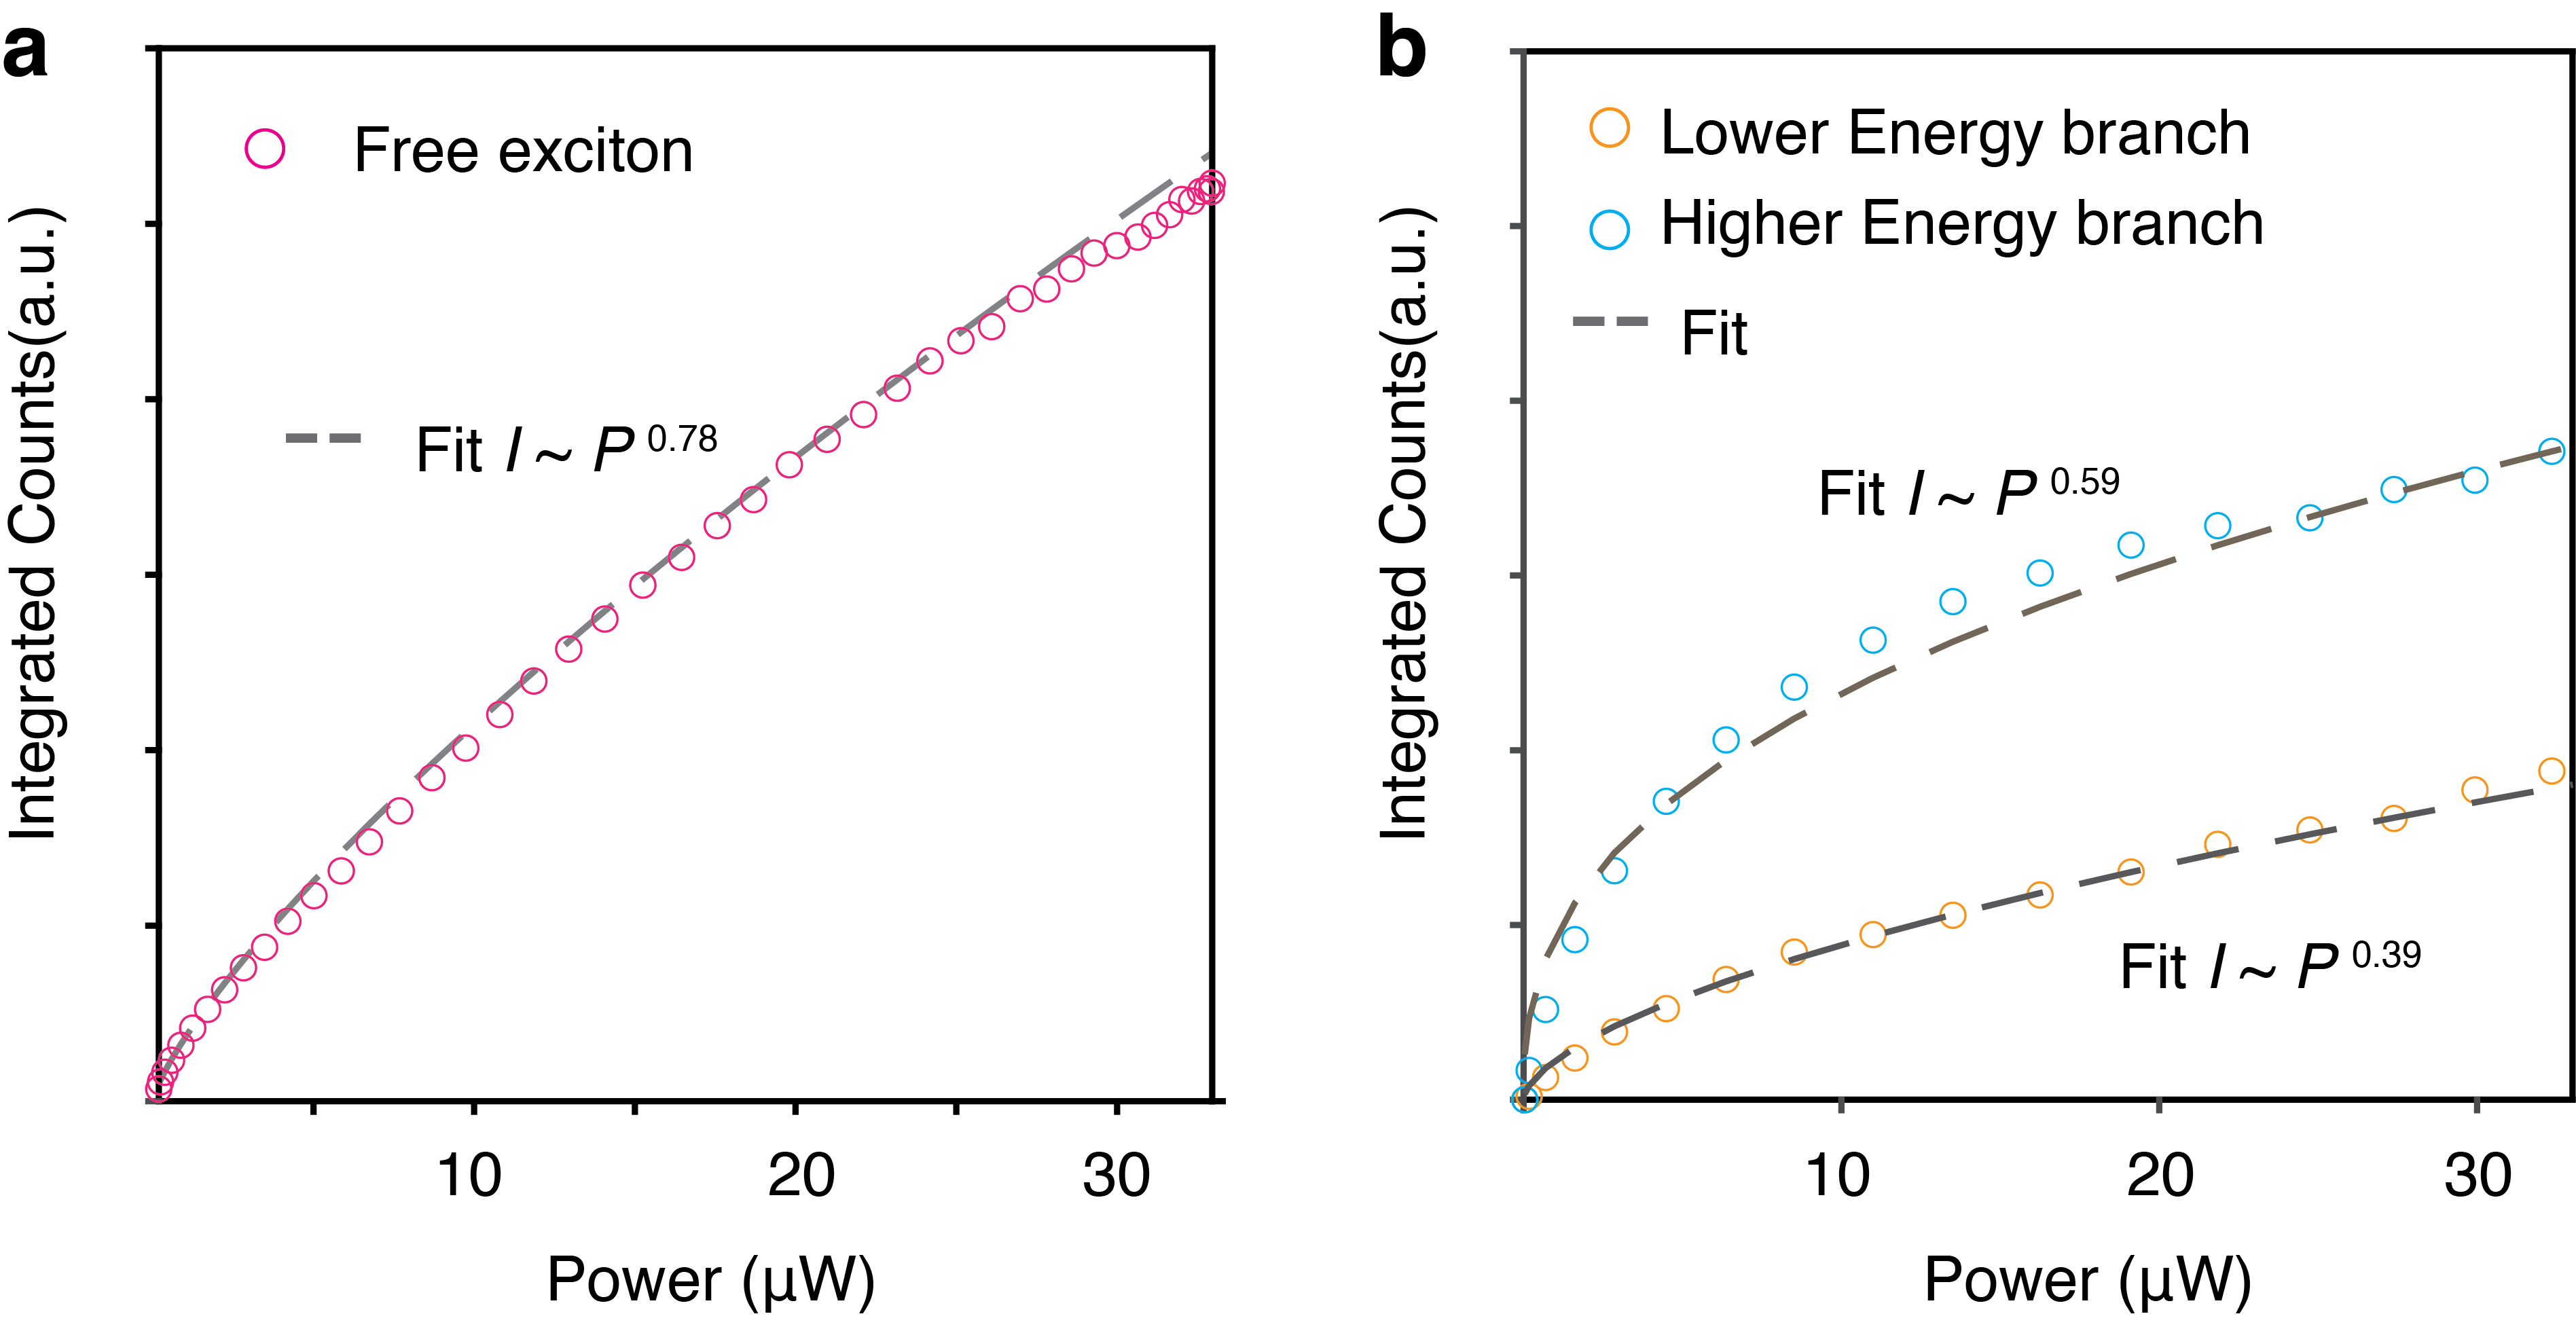
\includegraphics[width=0.7\textwidth]{Figures/C4/figure-S6.jpg} % 
\end{center}
\caption[power dependent] {\textbf{Excitation power–dependent PL intensities of free and 1D-confined excitons.} With increasing excitation power, \textbf{a,} the integrated PL intensity of free 2D excitons rises almost linearly, whereas \textbf{b,} the 1D-confined excitons exhibit sublinear saturation. Notably, the lowest-energy branch saturates significantly faster than the higher-energy branch.}
\label{fig.s6}
\end{figure}
\end{quote}
\renewcommand{\baselinestretch}{2}
\small\normalsize
% --------------
%///////////////////////Figure Panel End/////////////////////////

\subsection{Anisotropic Polarization of polarons and temperature-dependent}

Such quantum confinement also applies to charged excitons near DBs. 
In another MoSe$_2$ device, D2, we also observe a splitting in both the repulsive and the attractive polarons as we adjust the doping levels via gating (Figure~\ref{fig.s4}).
The reflectance of the neutral exciton, repulsive polaron, and attractive polaron all exhibit linear polarization parallel to the domain wall directions, indicating that 1D confinement can also occur for the Fermi polarons (Figures~\ref{fig.4-10} a-c).
Intriguingly, as doping density increases, the split between the repulsive polarons tends to decrease, whereas that between the attractive polarons slightly increases (Figure~\ref{fig.s4} b).
A quantitative understanding of the confinement of Fermi polarons requires further theoretical studies, for instance, on the polarizability of attractive vs. repulsive polarons \cite{Cavalcante2018-er}. 
Nevertheless, such behaviors stand in stark contrast to strain-induced energy splitting, which is expected to be independent of doping. 

To further demonstrate the robustness of this confinement, we measure the polarization-resolved reflectance of the neutral excitons at different temperatures. 
The anisotropic excitonic response persists but becomes weaker with increasing temperature. 
At temperatures around 80 K, where the thermal energy becomes comparable to the confinement potential, the two split exciton peaks merge into a single free exciton peak. 
The reflection and emission from excitons also become isotropic in the 2D plane above this temperature. 
We note that the disappearance of the splitting is not simply due to the linewidth change because the total linewidth does not change dramatically with increasing temperature up to 100 K (Figure~\ref{fig.s5}). 

%////////////////////////////Figure Panel//////////////////
%Fig.9(s4)--------------
\renewcommand{\baselinestretch}{1}
\small\normalsize
\begin{quote}
\begin{figure}
\begin{center}
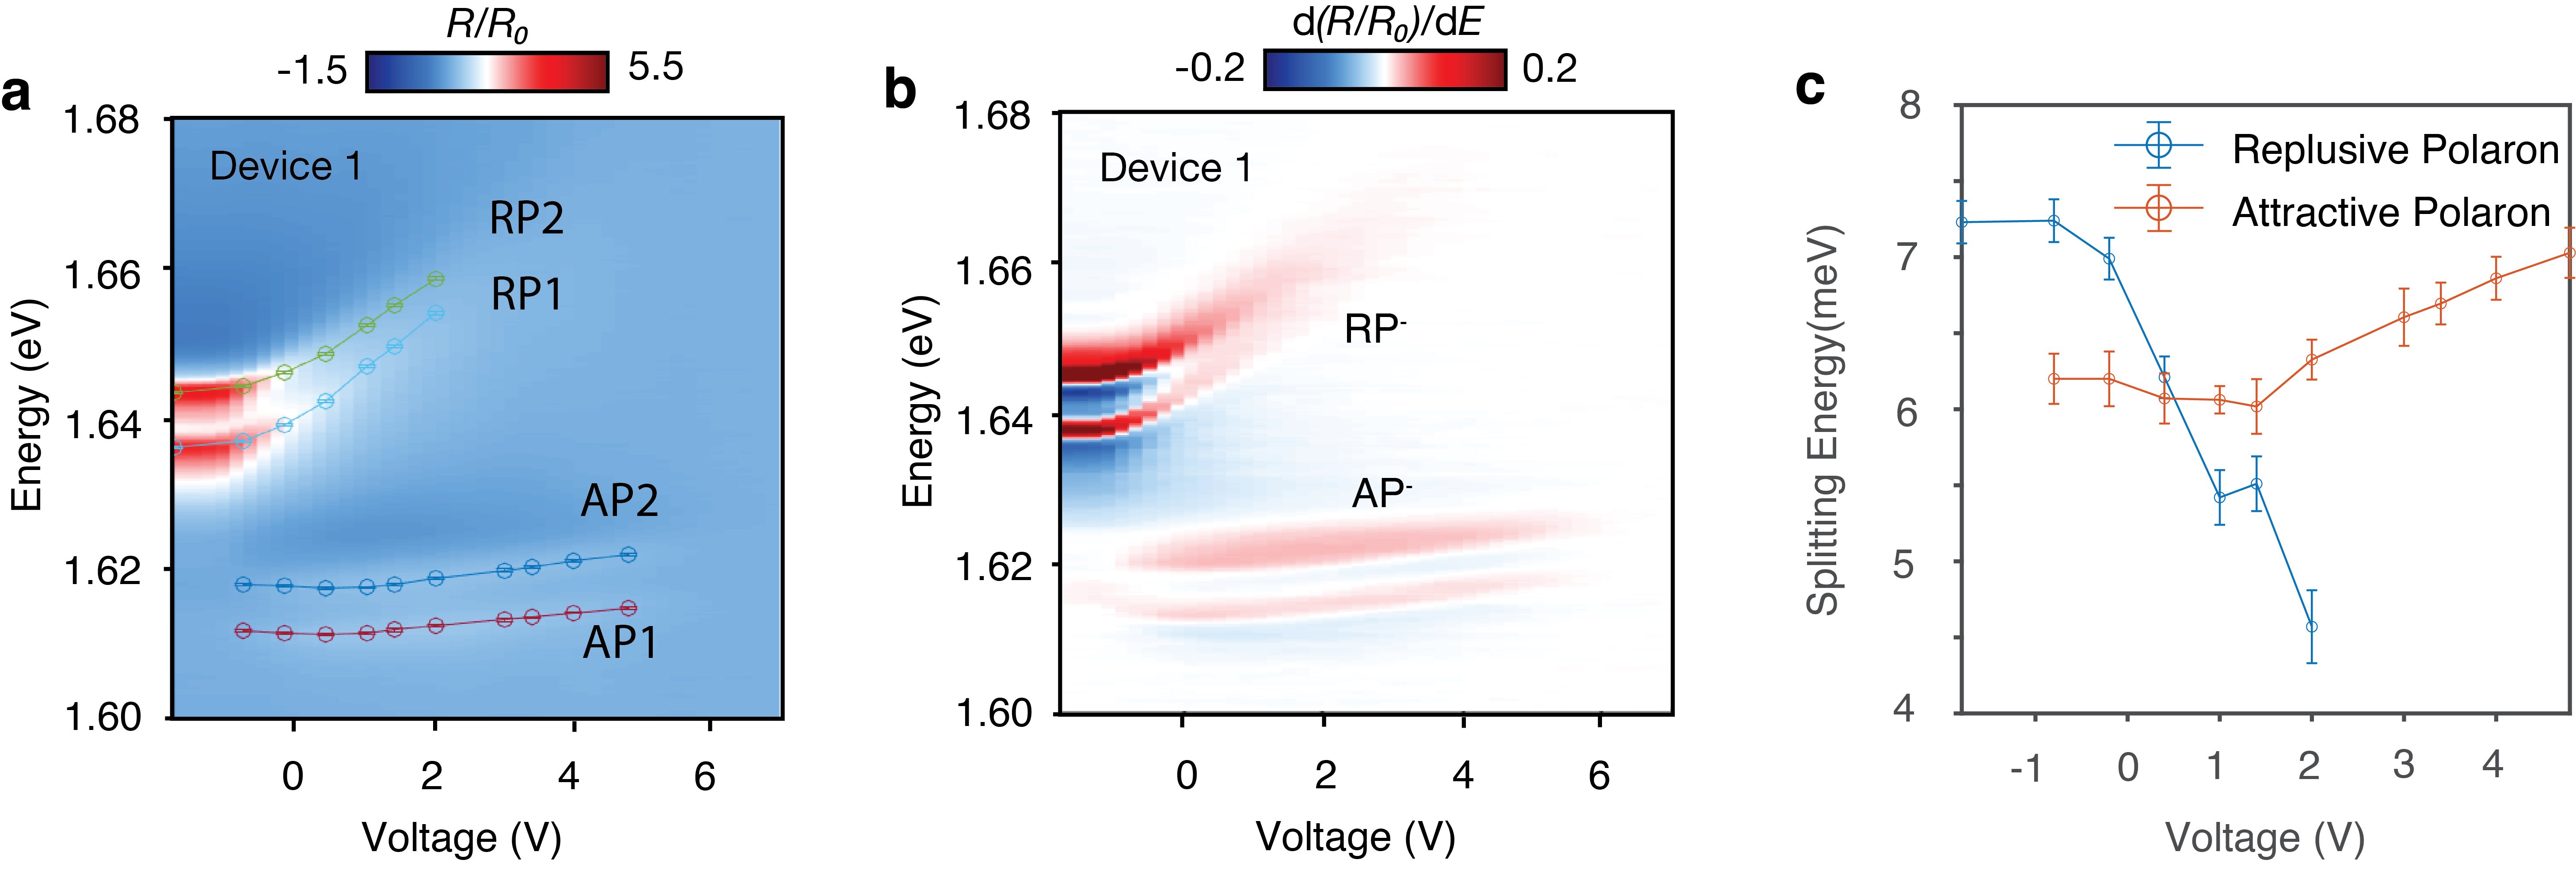
\includegraphics[width=1\textwidth]{Figures/C4/figure-S4.jpg} % 
\end{center}
\caption[gate polarons] {\textbf{Confinement of repulsive and attractive polarons.} Doping dependence of \textbf{a,} normalized reflectance, and \textbf{b,} its derivative with respect to energy. 
\textbf{c,} The energy splitting of the repulsive and attractive polarons exhibit different dependence on the doping level. The error bars represents the uncertainty in determining the peak position by Gaussian fit.}
\label{fig.s4}
\end{figure}
\end{quote}
\renewcommand{\baselinestretch}{2}
\small\normalsize
% 

%Fig.10(4)--------------
\renewcommand{\baselinestretch}{1}
\small\normalsize
\begin{quote}
\begin{figure}
\begin{center}
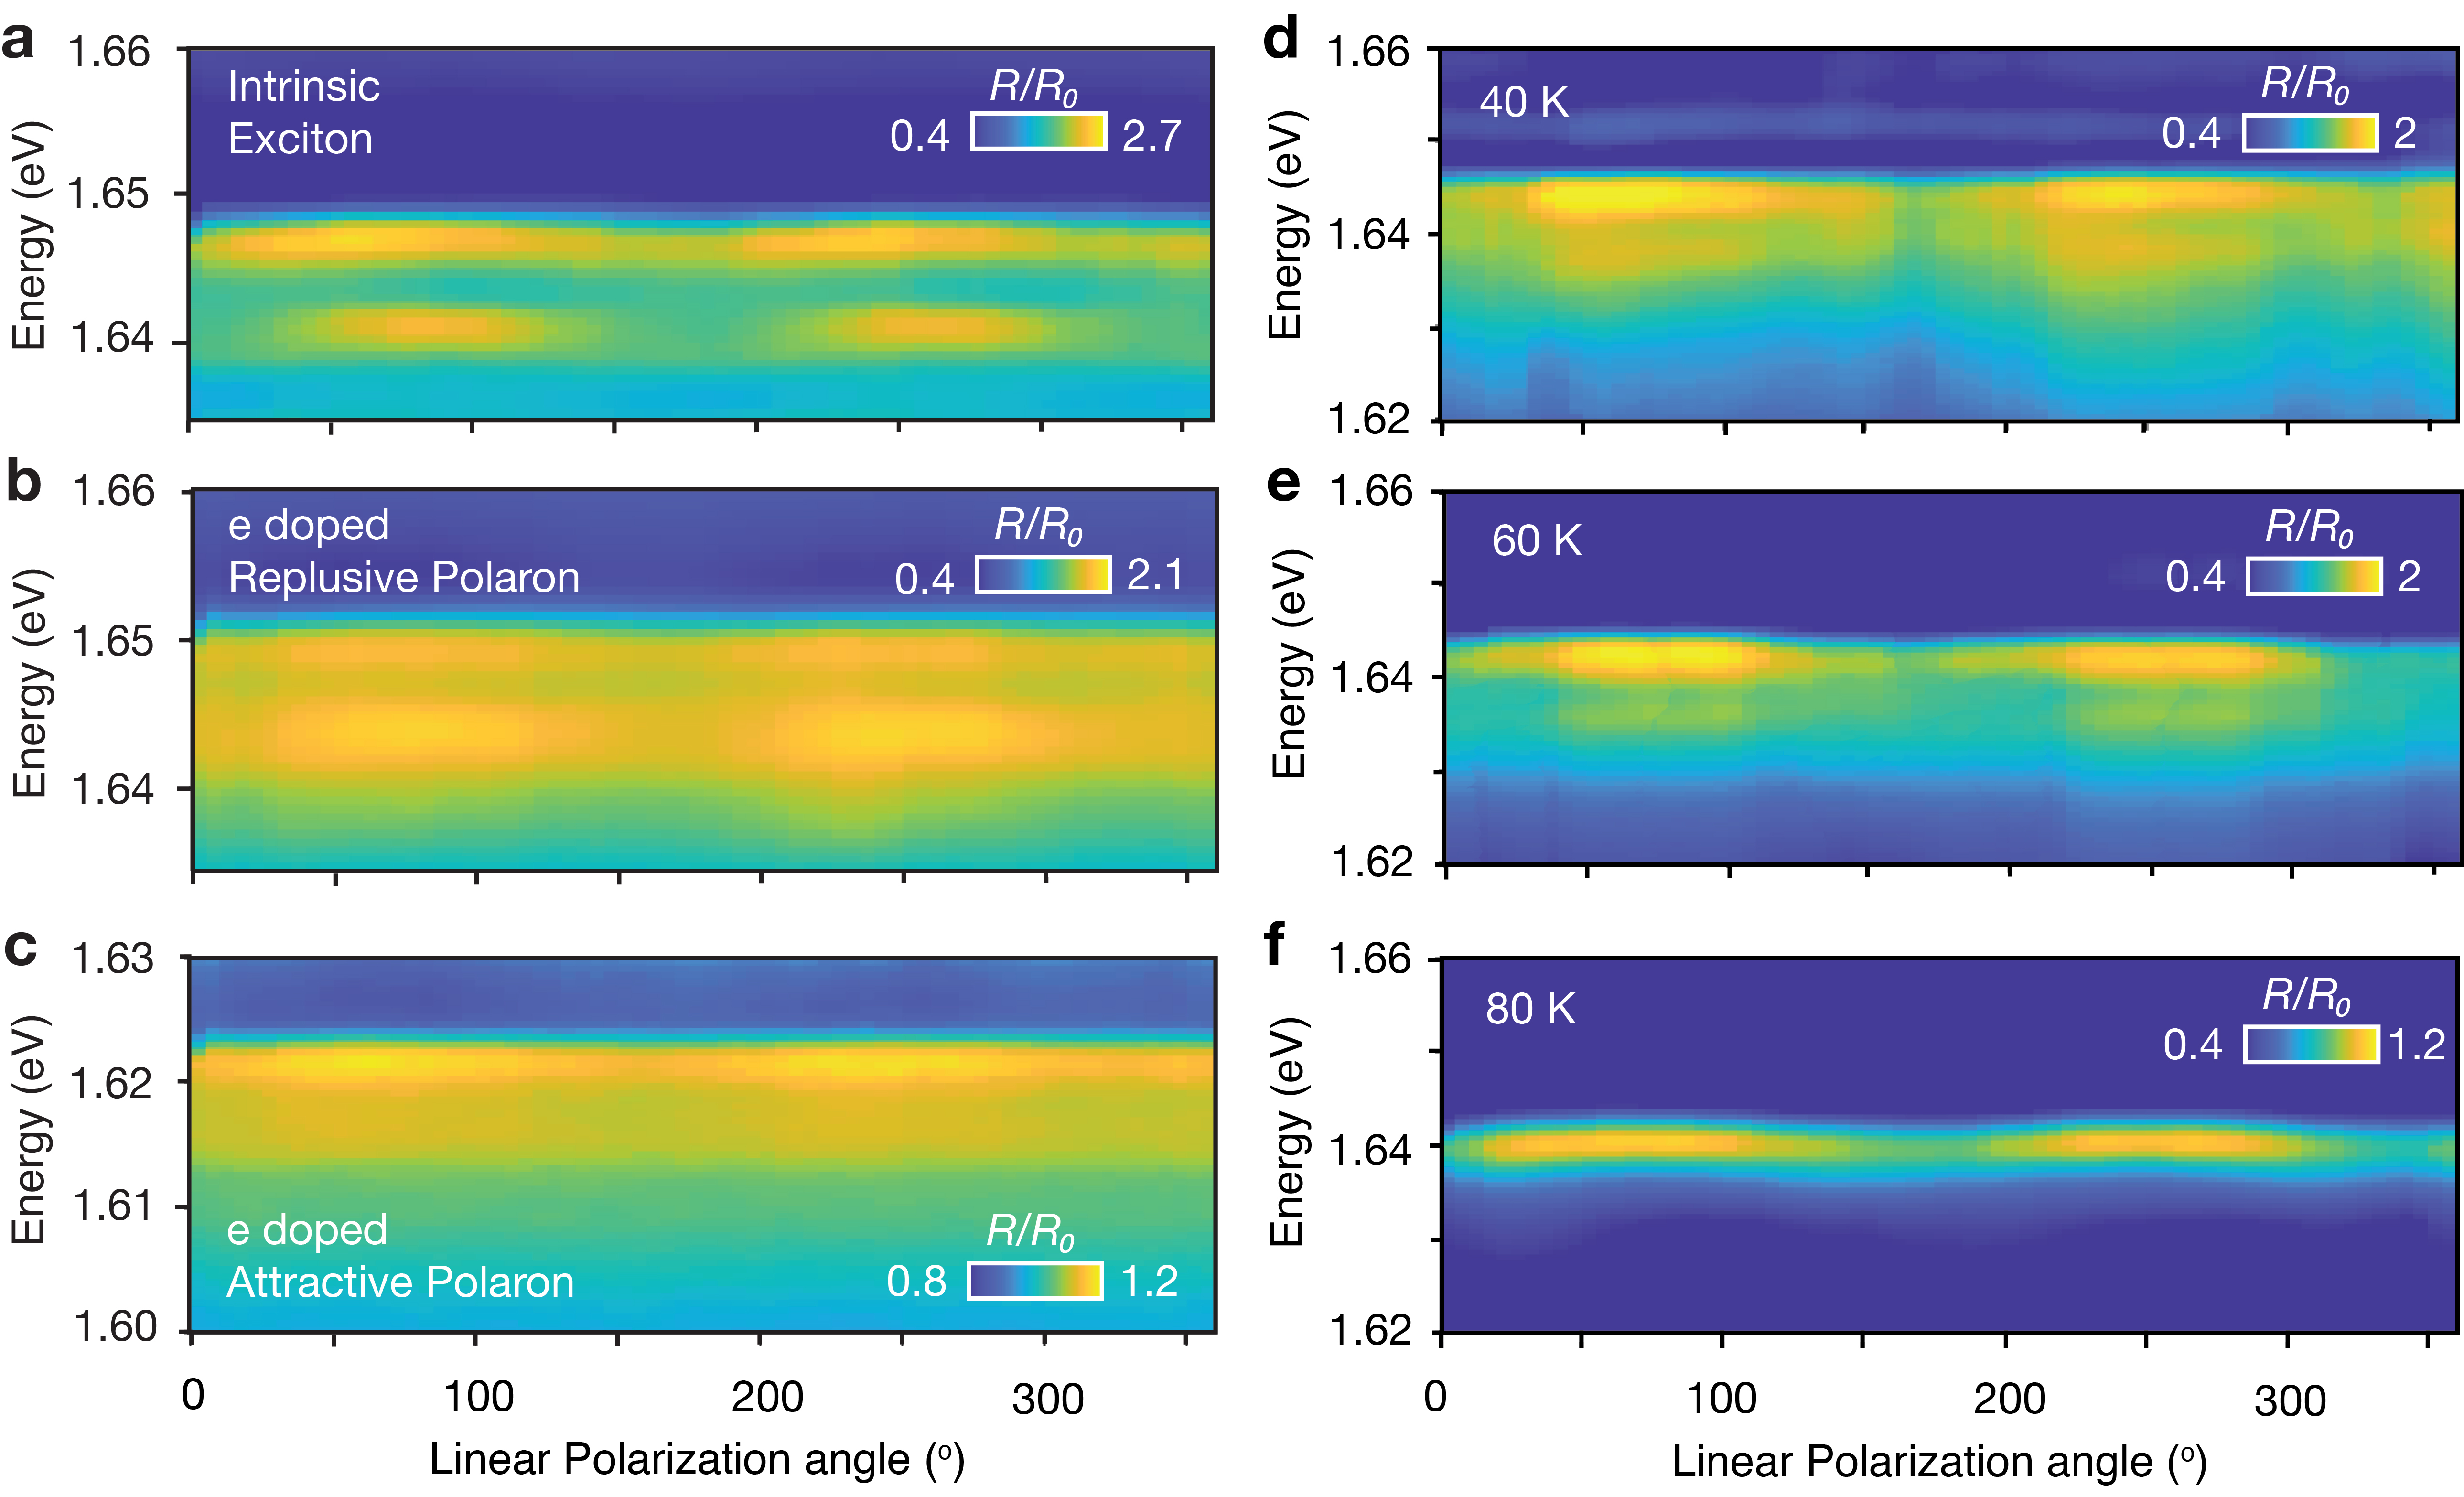
\includegraphics[width=0.9\textwidth]{Figures/C4/figure4-9.jpg} % 
\end{center}
\caption[gate polarons polarization] {\textbf{Anisotropic optical response of Fermi polarons and their temperature dependence.} \textbf{a-c,} Linear polarization dependent reflectance of a, neutral exciton (at gate voltage \textit{V} =-2.5 V), \textbf{b,} repulsive polaron, and \textbf{c,} attractive polaron (at gate voltage \textit{V} =0.5 V) at electron-doped in MoSe$_2$ in device \textbf{D2} at 5 K. \textbf{d-f,} Linear polarization dependent reflectance of neutral exciton at different temperatures.}
\label{fig.4-10}
\end{figure}
\end{quote}
\renewcommand{\baselinestretch}{2}
\small\normalsize
% 

%Fig.11(s5)--------------
\renewcommand{\baselinestretch}{1}
\small\normalsize
\begin{quote}
\begin{figure}
\begin{center}
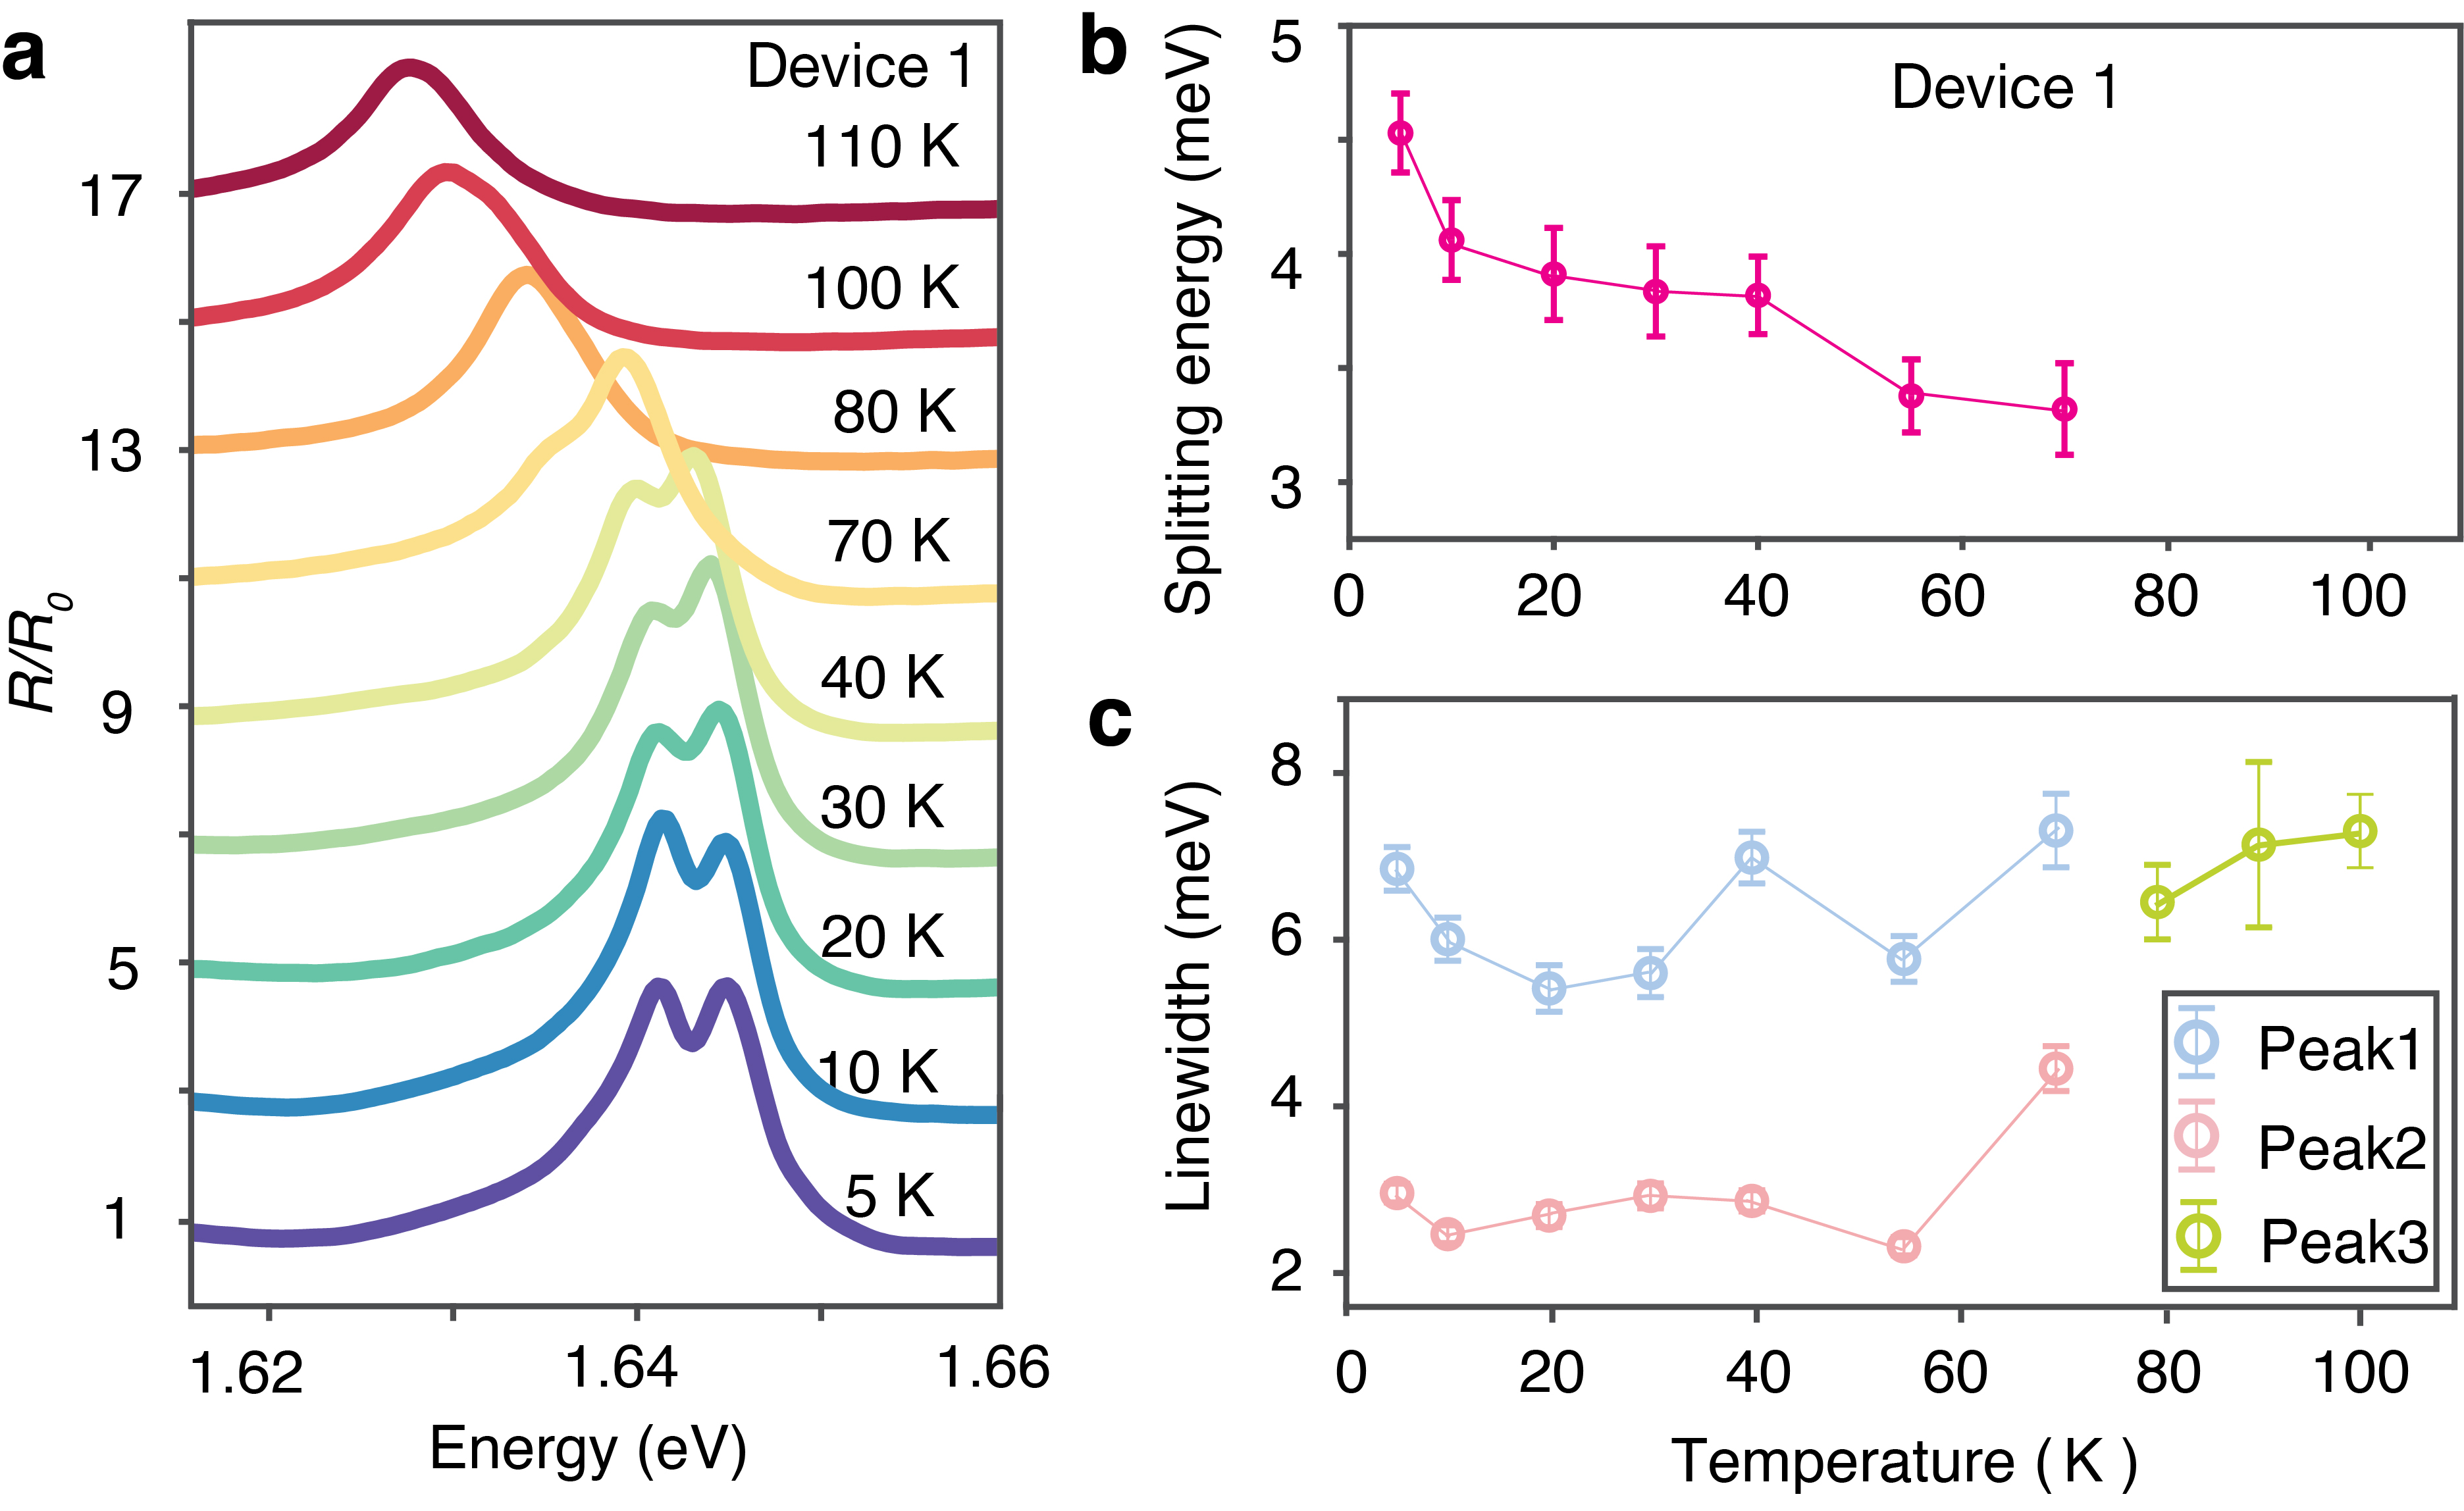
\includegraphics[width=0.9\textwidth]{Figures/C4/figure-S5.jpg} % 
\end{center}
\caption[Temperature dependent QC] {\textbf{Temperature-dependent quantum confinement.} \textbf{a-c,} \textbf{a,} Normalized reflectance of the intralayer excitons at different temperatures. With increasing temperature, each spectrum is shifted by a constant. \textbf{b,} The splitting energy decreases with increasing temperature and eventually vanishes near 80 K. \textbf{c,} The extracted linewidth as a function of temperature. Below 100 K, the linewidth does not change significantly, suggesting that the observed reduction in the splitting energy is not simply due to the linewidth change. The error bars represent the uncertainty associated with the fitted parameters of a Lorentzian model.}
\label{fig.s5}
\end{figure}
\end{quote}
\renewcommand{\baselinestretch}{2}
\small\normalsize
%////////////////////////////Figure Panel End//////////////////

\section{Discussions}

Finally, we quantify the strength and spatial extent of the quantum confinement potential. 
The potential depth induced by the in-plane electric field is given by Eq.~\ref{eq:stark}, 
where $\alpha\sim 6.5~\text{eV}\,\text{nm}^2/\text{V}^2$ for intralayer excitons in monolayer MoSe$_2$\cite{Thureja2022-yc,Cavalcante2018-er}. 
By modelling the electrostatic field generated by twisted hBN and solving the Schrödinger equation of excitons, we find the exciton confinement potential can reach a few to ten meVs, leading to two energy eigenstates with an energy splitting consistent with our experimental observations (Figure~\ref{fig.s8}). 
This potential is slightly deeper than those reported in recent experiments utilizing twisted hBN\cite{Kim2025-jv,Kiper2025-ao} and the electrostatic gated devices\cite{Heithoff2024-su,Thureja2022-yc}, but weaker than that inside the moiré superlattices16, as one may expect. 
Additionally, we estimate the lateral size of the confinement to be $\sim$ 4 nm, slightly smaller than the moiré DB size in the PFM images, possibly due to the limited PFM resolution. 
These results indicate that such electrostatic moiré potential imposes stronger and tighter confinement than in partially gated devices\cite{Hu2024-ua, Heithoff2024-su,Thureja2022-yc,Wang2018-tm,Thureja2024-og}. 
While strain can also be used to modify exciton energies and induce anisotropic diffusion\cite{Dirnberger2021-xd}, realizing one-dimensional, quantum-confined excitons under strain remains a challenge due to the difficulty of controllably applying nanoscale strain gradients.

Notably, the linewidth of such confined excitons is comparable to that of free excitons and exceeds some previously reported values in certain confined systems\cite{Hu2024-ua,Thureja2022-yc,Seyler2019-ok,Liu2021-hj}. 
Unlike zero-dimensional (0D) confinement, such as in moiré superlattices\cite{Seyler2019-ok,Liu2021-hj}, excitons in our system are restricted only along one dimension, resulting in large radiative broadening. 
Additionally, far-field measurements integrate signals from the entire 1D edge, leading to inhomogeneous broadening related to variations in disorder, domain boundary sizes, and electrostatic field, making it comparable to that of free excitons. 
Further improvement of the fabrication techniques is required to further reduce such inhomogeneous broadening.

\subsection{Estimation of the In plane Electric field and Confinement Potential}

We estimate the in-plane electric field distribution in the proximated MoSe$_2$ monolayer induced by the electrostatic potential drop of the underneath AB/BA domain boundary at the twisted hBN interface. 
The potential difference is related to the formed superlattice period \textit{b} and the distance between the superlattice interface and the top surface \textit{b}, which can be expressed as\cite{Zhao2021-cm}:
\begin{equation}
V(\mathbf{R}, z) \simeq \operatorname{sgn}(z)\,
\frac{P(\mathbf{R})}{2 \varepsilon_{0}}\,
e^{-G|z|}
\end{equation}
Where $P(\mathbf{R})$ is the laterally modulated net electrical polarization, $\mathbf{R}$ refers to the real local position. 
$G = \frac{4\pi}{\sqrt{3}\,b}$. 
When the superlattice period \textit{b} is large and distance \textit{z} is small ---$G|z| \ll 1$, the potential strength can be expressed as
\begin{equation}
\Delta V = V_{\max} - V_{\min} = \frac{P_{\max}}{\varepsilon_{0}}
\label{eq:potential_strength}
\end{equation}
where $P_{\max}$ is the calculated electrical polarization in AB-stacked twisted hBN at the position $r = \tfrac{2a}{\sqrt{3}}$, with $a$ being the lattice constant of hBN.
According to this, we obtained a potential difference of $254.1~\text{mV}$, with the top hBN thickness ($z$) of $2~\text{nm}$ and a supercell periodicity ($b$) of $1000~\text{nm}$. 
This would induce a Gaussian-distributed electric field at the domain boundary with a peak amplitude of $\sim 33.8 \pm 6~\text{mV}/\text{nm}$ and a domain width of $6 \sim 8~\text{nm}$.

We then apply the calculated peak electric field to build the quantum harmonic potential trap and calculate the exciton center-of-mass wave functions. 
We obtained in total two eigenstates confined in this harmonic trap, with a confinement length $l_x$ of $4.3~\text{nm}$ extracted 
from the FWHM of the ground-state eigenfunction as
$l_x = \frac{\mathrm{FWHM}}{2\sqrt{\ln 2}}$
This value can be compared to the confinement length estimated using a harmonic oscillator approximation based on the measured exciton energy splitting. 
The confinement length is given by $l \sim \frac{\hbar}{\sqrt{m_X \Delta E}}$, where $m_X \sim 1.3\,m_e$. This gives a confinement length of about $4.1~\text{nm}$ with a discrete energy splitting of $3.5~\text{meV}$.

%////////////////Figure////////////////
%Fig.12(s8)--------------
\renewcommand{\baselinestretch}{1}
\small\normalsize
\begin{quote}
\begin{figure}
\begin{center}
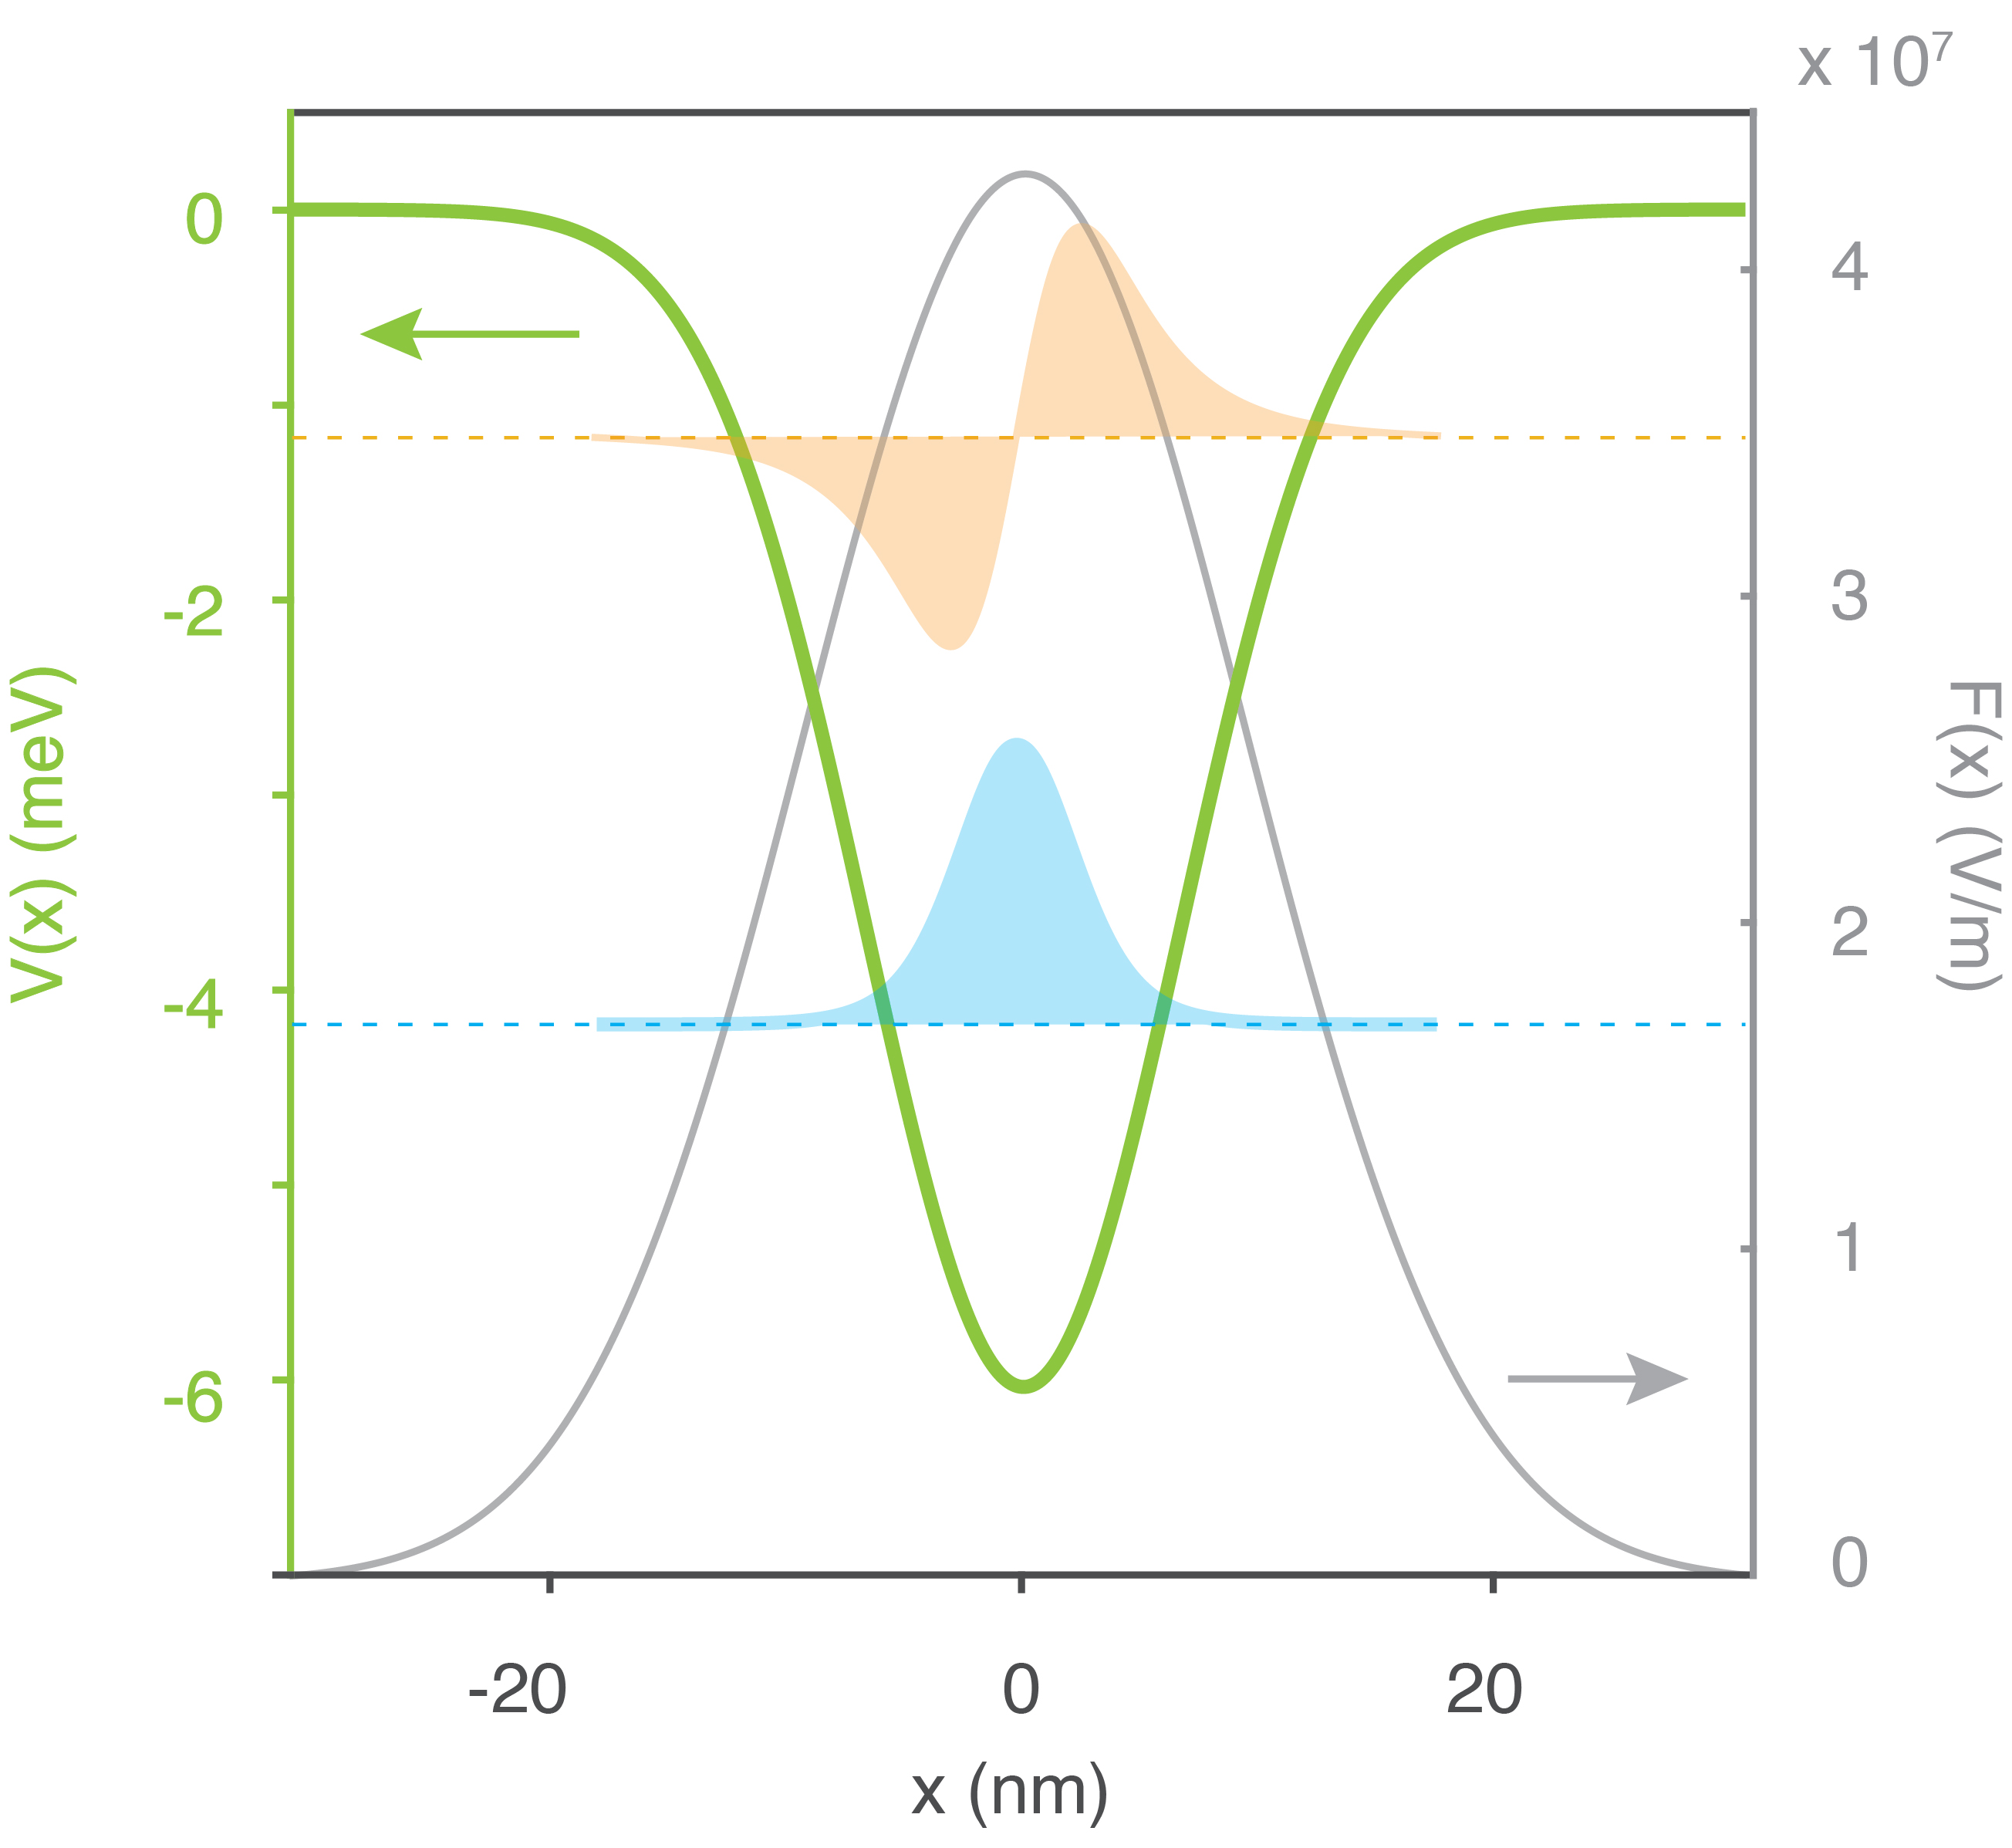
\includegraphics[width=0.5\textwidth]{Figures/C4/figure-S8.jpg} % 
\end{center}
\caption[potential well calculation] {Calculated in-plane electric field \textit{F}(x) (in grey line), confining potential \textit{V}(x) (in green line), and the exciton eigenstates at the 1 $~\mu$m domain region.}
\label{fig.s8}
\end{figure}
\end{quote}
\renewcommand{\baselinestretch}{2}
\small\normalsize
%////////////////Figure End////////////////

\section{Conclusions}

We exploit the recently discovered moiré ferroelectricity in twisted hexagonal boron nitride (hBN) to imprint nanoscale potentials on excitons in 2D semiconductors. 
The strong in-plane electric fields localized at the moiré domain boundaries (DBs) modify the optical reflectance of  MoSe$_2$, indicating that excitons can be confined within a strips as narrow as $\sim$ 10 nanometers. 
The quasi-one-dimensional nature of this confinement is further evidenced by the linear polarization of their optical reflectance. 
In addition, the same fields impose even stronger confinement on Rydberg excitons due to their larger polarizability.

The demonstrated quantum confinement of intralayer excitons at moiré domain walls opens exciting new avenues for controlling excitons at the nanoscale. 
Such a strong in-plane electric field is expected to occur in many types of twisted hetero-structures with broken inversion symmetry \cite{Sung2020-ru}, which can be readily integrated with all sorts of 2D semiconductors to engineer their electronic and excitonic properties\cite{Akamatsu2021-uo,Hu2023-px,He2024-se,Zhang2024-zi}. 
The ferroelectric response observed in many of such twisted structures could enable dynamic electrical control of 1D exciton chains\cite{Kim2025-jv,Vizner-Stern2021-gx,Yasuda2024-qd}. 
The excitonic potential imposed by such an electrostatic lattice — ranging from a few to tens of millielectronvolts — can be tuned to be comparable to the exciton interaction strength\cite{Gu2024-en,Datta2022-po,Tagarelli2023-an,Gu2021-cu,Wang2018-pz}. 
This opens intriguing opportunities for investigating how the interplay between confinement and correlation can give rise to emergent properties in strongly interacting many-body quantum systems, such as quantum optical nonlinearity. 
By employing Rydberg excitons, one can access a compelling regime in which the confinement length scale is comparable to the exciton blockade radius, analogous to one-dimensional Rydberg atom chains\cite{Endres2016-zd,Firstenberg2013-to,Roy2017-nd}. 
To access this intriguing regime, new optical methods may be required to investigate how light interacts with the 1D excitonic chains as it propagates along and within the domain walls, such as near-field techniques\cite{Zhang2022-ty,Crottini2001-lg}.
%Chapter 5

\renewcommand{\thechapter}{5}

\chapter{Interlayer exciton and optical nonlinearity of Fermi polaron in Trilayer WSe$_2$}
\label{chap5}

Realizing strong nonlinear optical responses is a long-standing goal of both fundamental and technological importance. Recently significant efforts have focused on exploring excitons in solids to achieve nonlinearities even down to few-photon levels. 
However, a crucial tradeoff arises as strong light-matter interactions require large oscillator strength and short radiative lifetime of excitons, which limits their nonlinearity. 
Here we experimentally demonstrate strong nonlinear optical responses with large oscillator strength by exploiting the coupling between excitons and carriers in an atomically thin semiconductor. 
By controlling the electric field and electrostatic doping of trilayer $WSe_2$, we observe the hybridization between intralayer and interlayer excitons and the formation of Fermi polarons. 
Substantial optical nonlinearity is observed under continuous wave and pulsed laser excitation, where the Fermi polaron resonance blueshifts by as much as ~10 meV. 
Intriguingly, we observe a remarkable asymmetry in the optical nonlinearity between electron and hole doping, which is tunable by the applied electric field.
We attribute these features to the optically induced valley polarization due to the interactions between excitons and free charges. 
Our results establish atomically thin heterostructures as a highly versatile platform for engineering nonlinear optical response with applications to classical and quantum optoelectronics.

\section{Introduction}
Nonlinear optical phenomena lie at the heart of classical and quantum optics, with applications ranging from data communications to quantum control\cite{Volz2012-pb,Boyd2020-re}. 
Developing physical systems with stronger optical nonlinearity while reducing their power requirement holds the promise for more efficient optoelectronics and may unlock new technologies such as single-photon switches and transistors\cite{}. 
In recent years, significant efforts have been devoted to investigating excitons in semiconductors as a solid-state medium for realizing strong optical nonlinearity1–3.
Van der Waals heterostructures based on atomically thin transition metal dichalcogenides (TMDs) have emerged as a new platform for fundamental studies of excitons and for engineering optical responses9,10. Excitons in such two-dimensional materials are highly tunable with rich spin-valley physics and possess characteristics promising for optical nonlinearity, such as strong light-matter interactions and weak screening of Coulomb potential10. 
However, a major challenge in achieving high nonlinearity under low excitation power arises from the balance between the strengths of exciton-photon and exciton-exciton interactions11–13. 
For instance, intralayer excitons in these materials exhibit large oscillator strength but experience weak interactions, dominated by exchange interactions and limited by their short lifetime14. 
On the other hand, interlayer excitons in TMD heterostructures have longer lifetimes and experience interactions due to their finite electric dipole moment15,16. 
Unfortunately, spatial separation of the electron-hole wavefunctions leads to weaker absorption of incident photons. 
Several recent studies demonstrated enhanced the interlayer exciton absorption via its hybridization with intralayer excitons in $MoS_2$1,17–19, although the oscillator strength of such hybrid excitons is still an order of magnitude weaker than the intralayer ones. 
So far, strong nonlinearity in the intralayer excitons has not yet been realized.
In this study, we report giant nonlinear optical responses of intralayer charged excitons, i.e., Fermi polarons, on the order of several millielectronvolts under photon flux of 1013 photons per second per square micrometer. 
The strong nonlinearity is highly tunable by doping and electric field, based on which we attribute the nonlinearity to an optically induced valley polarization resulting from exciton-carrier scattering.

\section{Sample Fabrication}
Graphite, hBN flakes are mechanically exfoliated from the bulk crystals onto the silicon chip with $SiO_2$ layer. 
Some of the exfoliated homotrilayer $WSe_2$ flakes were provided by the Quantum material press (QPress) facility in Center for functional nanomaterials (CFN) at Brookhaven national laboratory (BNL). 
The thickness of the hBN flakes and $WSe_2$ layer numbers are estimated based on the color contrast under the optical microscopy. 
The heterostructure is assembled in a transfer station built by Everbeing Int’l Corp., which use PDMS(Polydimethylsiloxane) and PC (Polycarbonate) as stamp and transfer all the flakes in a dry transfer method onto a silicon chip with 285nm $SiO_2$ layer. 
Then the electrical contacts are patterned by electron-beam lithography and a liftoff process where we deposited 5nm of Cr and 80 nm of Au by thermal evaporation.
Figure~\ref{fig.5.1} shows the device schematic and the fabricated device optical image under 100 X magnification. 

%////////////////////////////Figure Panel//////////////////
%Fig.5.1--------------
\renewcommand{\baselinestretch}{1}
\small\normalsize
\begin{quote}
\begin{figure}
\begin{center}
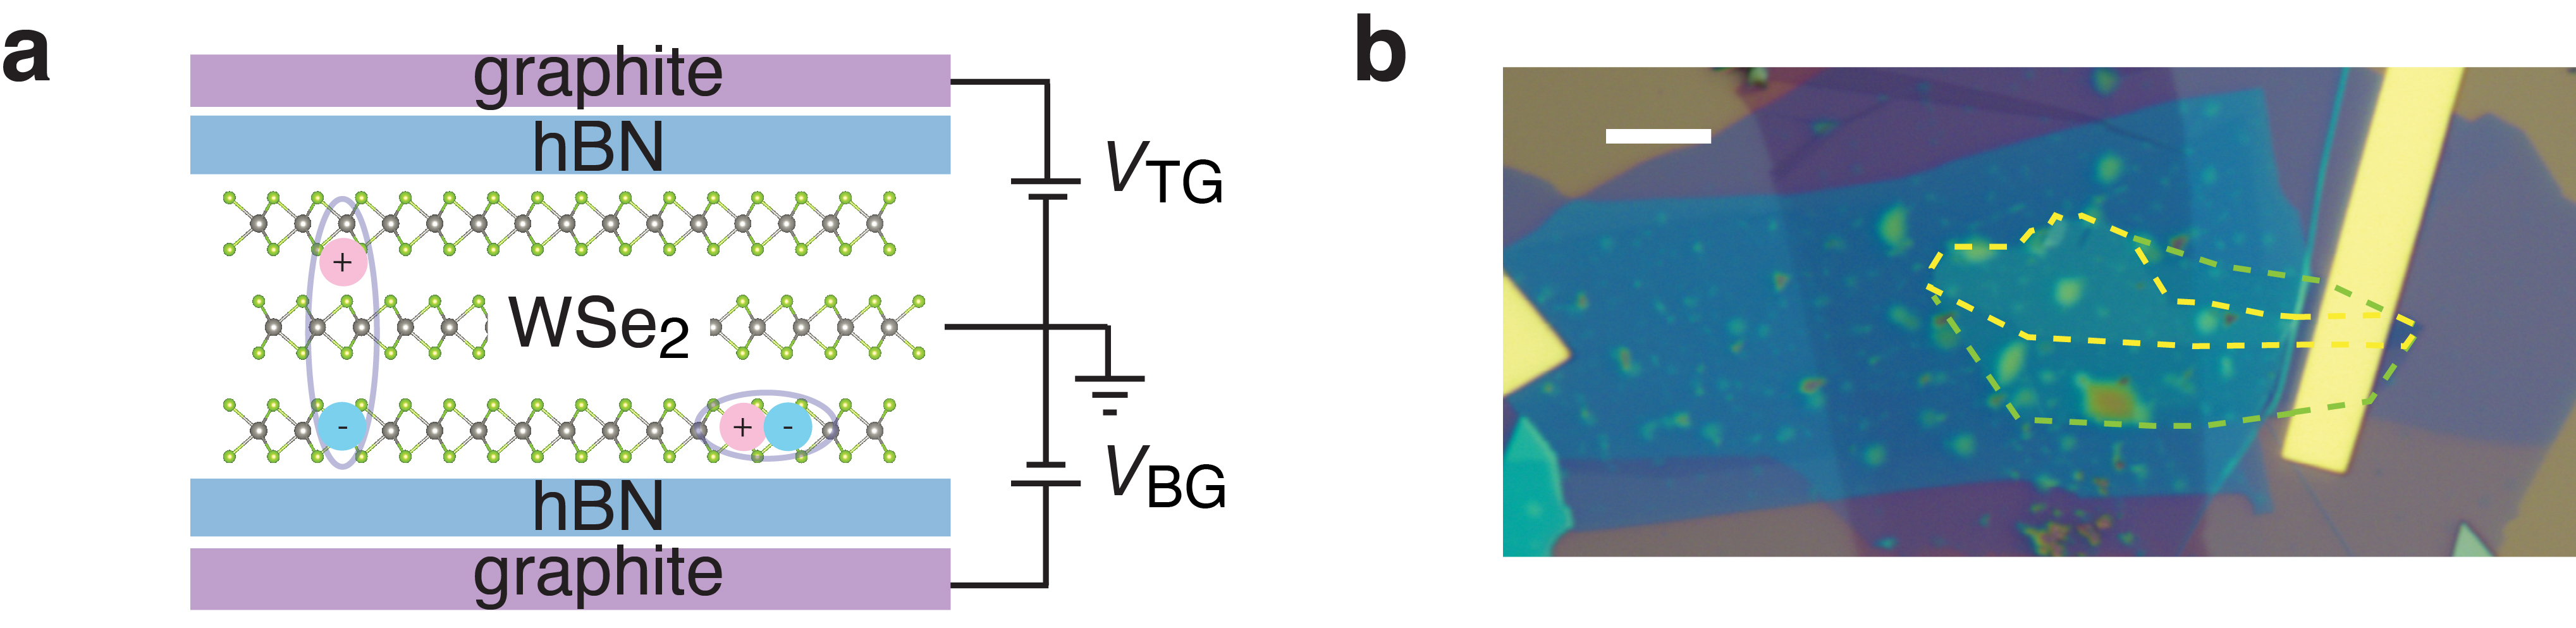
\includegraphics[width=1\textwidth]{Figures/C5/Fig5_1.jpg} % 
\end{center}
\caption[Dual-gated WSe$_2$ homotrilayer van der Waals heterostructure] {\textbf{Dual-gated WSe$_2$ homotrilayer van der Waals heterostructure.} \textbf{a}, Schematic of the trilayer vdW heterostructure. 
The homotrilayer WSe$_2$ is encapsulated with two hBN layers of thickness 15-20 nm. 
\textbf{b}, Optical image of the homotrilayer WSe$_2$ device (scale bar: 5~$\mu$m). 
The trilayer and neighboring bilayer regions are enclosed by yellow and green dashed lines, respectively.}
\label{fig.5.1}
\end{figure}
\end{quote}
\renewcommand{\baselinestretch}{2}
\small\normalsize
% %///////////////////////
\section{Results and Discussions}
\subsection{Electrical control of excitons}
In our experiments, we encapsulate exfoliated WSe$_2$ homotrilayers inside two layers of hBN in a dual-gate geometry to independently control the overall doping levels and the displacement field (Figure~\ref{fig.5.2}). 
Figure~\ref{fig.5.2}a shows the photoluminescence (PL) map of the sample by varying the electric field while keeping the samples undoped. 
We observe strong emission from excitons XI, whose energy linearly shifts with electric field from 1.58 eV to 1.50 eV, and PL peaks at 1.71, 1.55 and 1.52 eV that remains constant with varying electric field. 
We attribute the peak at 1.71 eV to intralayer momentum-direct exciton X$_A$ at the K-K transition, based on their strong absorption (Figure~\ref{fig.5.2}b) and zero Stark shift. 

%////////////////////////////Figure Panel//////////////////
%Fig.5.2--------------
\renewcommand{\baselinestretch}{1}
\small\normalsize
\begin{quote}
\begin{figure}
\begin{center}
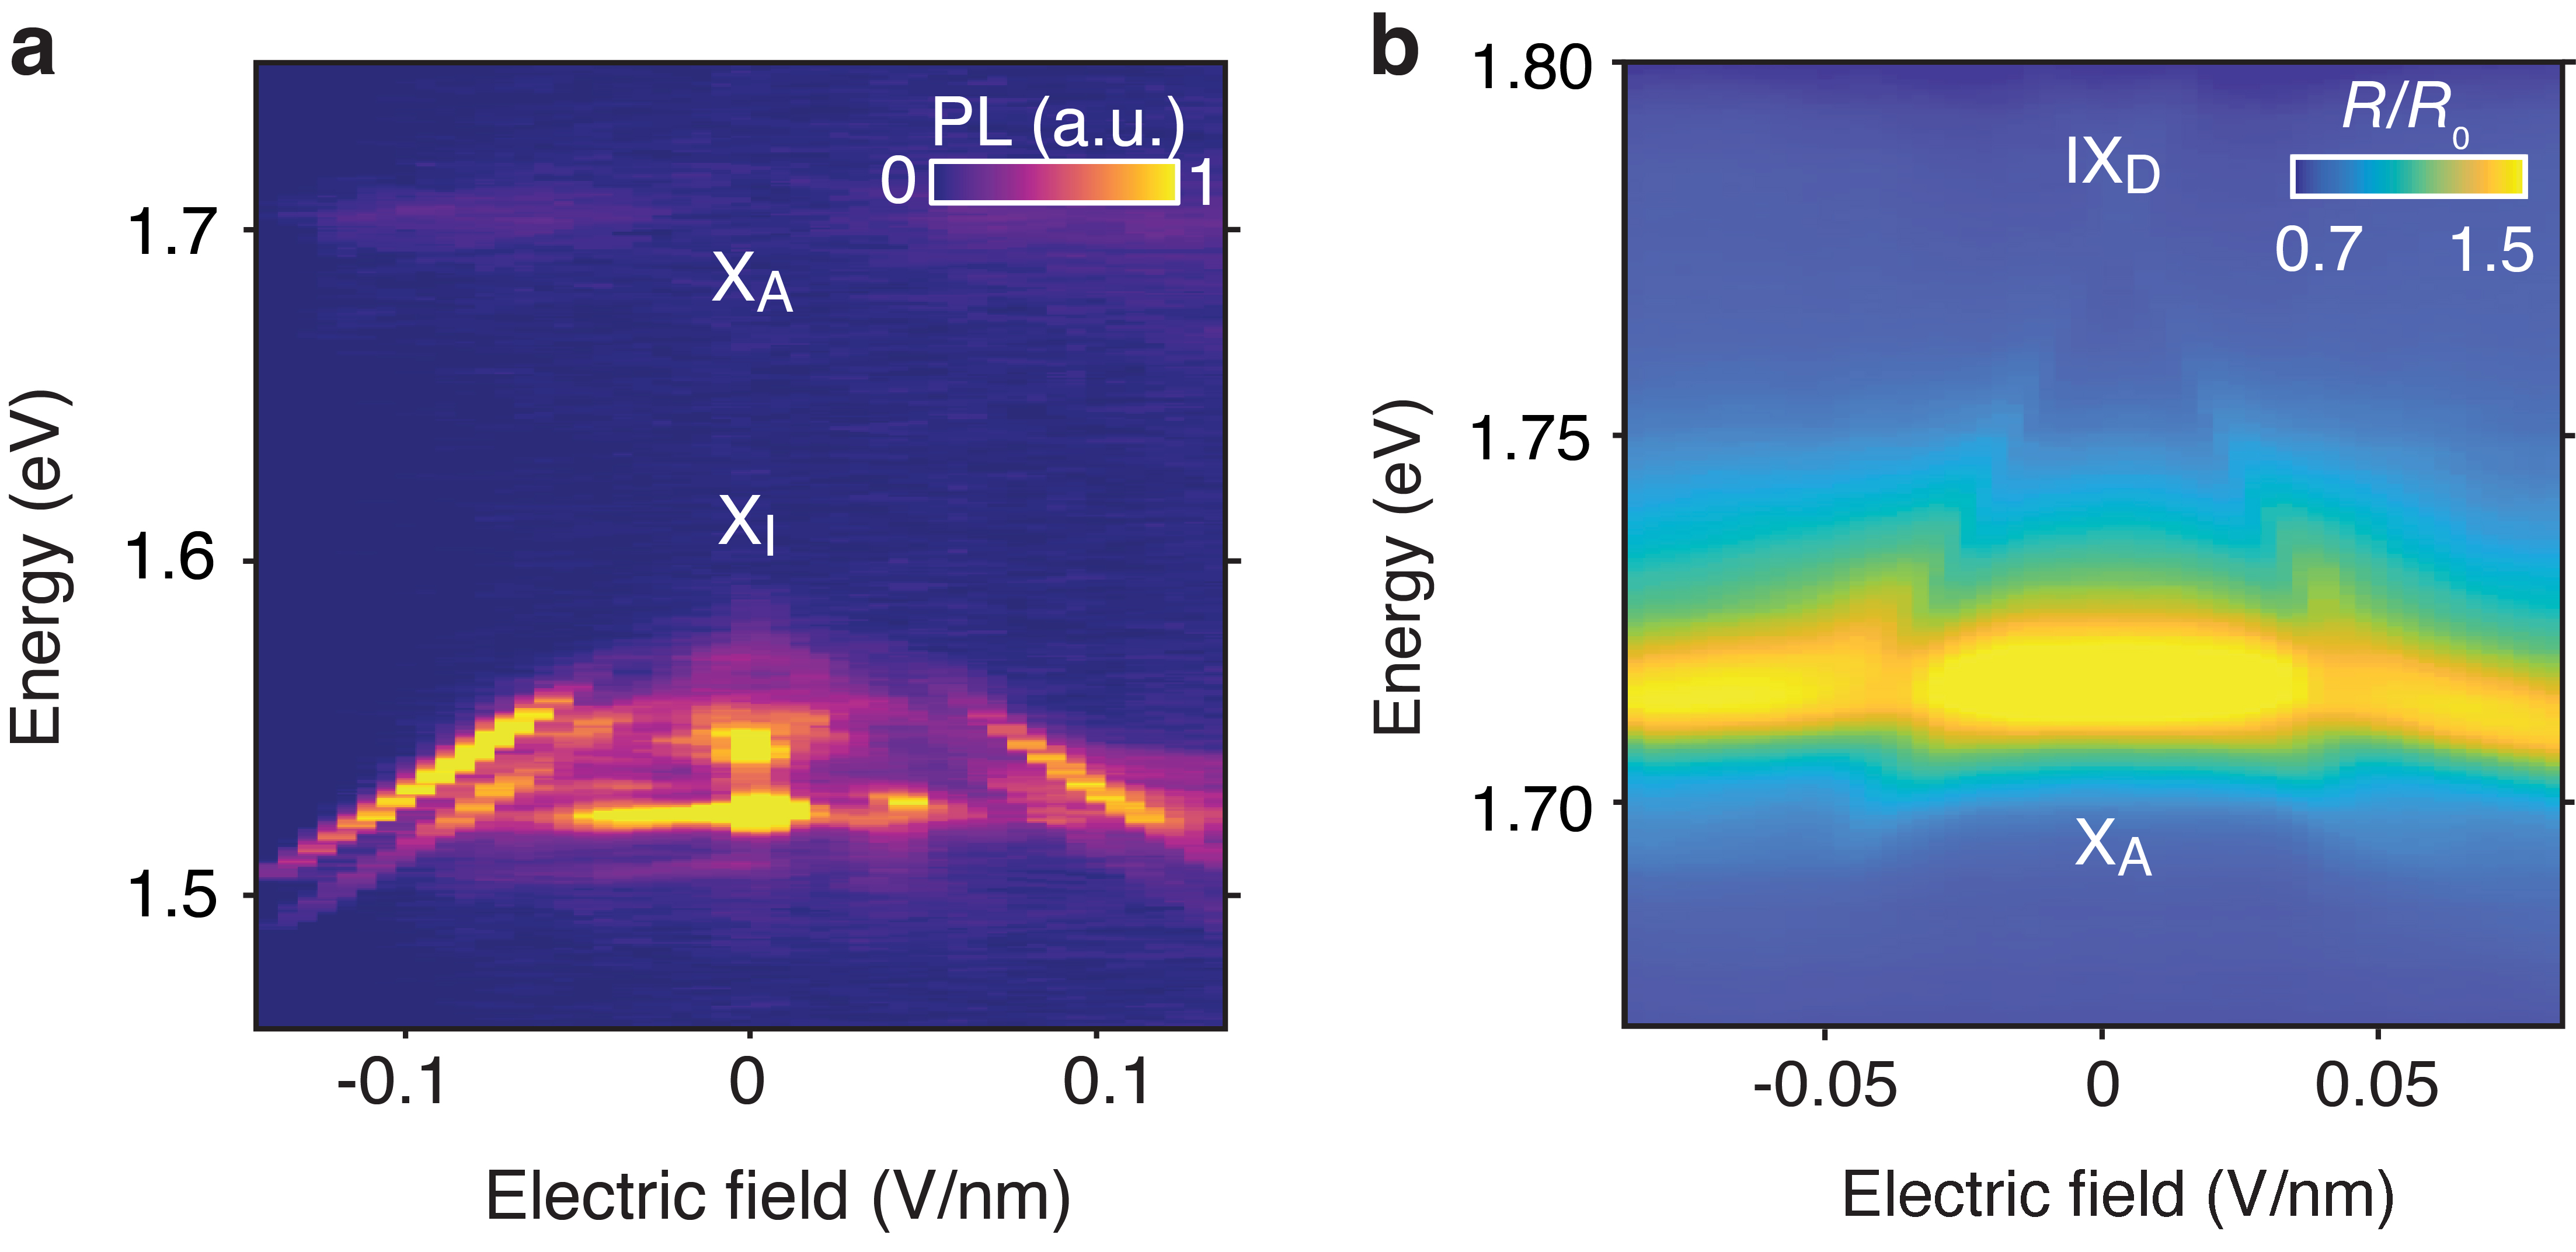
\includegraphics[width=0.85\textwidth]{Figures/C5/Fig5_2.jpg} % 
\end{center}
\caption[Optical characteristic of dual-gated homotrilayer WSe$_2$ van der Waals heterostructure.] {\textbf{Optical characteristic of dual-gated homotrilayer WSe$_2$ van der Waals heterostructure.} 
\textbf{a}, Photoluminescence spectra of the WSe$_2$ trilayer under an applied electric field. 
The bright emission at 1.50--1.58~eV, exhibiting a Stark shift with field, corresponds to the indirect exciton X$_I$. 
The weaker emission near 1.70~eV corresponds to the momentum-direct K--K intralayer exciton X$_A$.  
\textbf{b}, Reflectance spectra of the WSe$_2$ trilayer under an electric field. 
The high-energy momentum-direct K--K interlayer exciton exhibits a Stark shift of $\sim$100~meV and begins to hybridize with X$_A$ when their energies become degenerate around an electric field of $\sim$ 0.05 V/nm.}
\label{fig.5.2}
\end{figure}
\end{quote}
\renewcommand{\baselinestretch}{2}
\small\normalsize
% %///////////////////////

The lower energy of X$_I$ indicates that they are momentum-indirect excitons at the band edge, corresponding to transition across the indirect gap, located at the valence band $\Gamma$ and conduction band Q valleys, according to the band structure calculations20–22. 
From the linear Stark shift, we estimate the electric dipole of X$_I$.  
The energy shift as a function of the electric field of the IX$_D$ and X$_I$ obeys the law of the stark shift, which can be described as:
\begin{equation}
\Delta E = \lvert e \cdot d \cdot E \rvert 
= \left\lvert e \cdot d \cdot \frac{\varepsilon_{\mathrm{hBN}}}{\varepsilon_{\mathrm{WSe_2}}}
\cdot \frac{V_{\mathrm{BG}}}{t_{\mathrm{BG}}} \right\rvert 
\label{eq:deltaE}
\end{equation}
Thus the dipole moment of excitons can be calculated as:
\begin{equation}
d = \left\lvert 
\frac{\Delta E}{e} \cdot 
\frac{\varepsilon_{\mathrm{WSe_2}}}{\varepsilon_{\mathrm{hBN}}} \cdot 
\frac{t_{\mathrm{BG}}}{V_{\mathrm{BG}}} 
\right\rvert
\label{eq:d_expression}
\end{equation}
The estimated electric dipole of X$_I$ is around 0.78 $nm\cdot e$. 
The corresponding vertical displacement of the electron-hole pair in X$_I$ is approximately half of the distance between the top and bottom tungsten layers, indicating the electrons or holes are partially layer delocalized. 

Next, we measure the reflectance of the trilayer under an electric field (Figure~\ref{fig.5.2}b). 
In addition to the intralayer X$_A$, we observe an additional reflectance contrast at 1.78 eV (IX$_D$), which exhibits a substantial Stark effect of almost 100 meV (additional devices shown in Figure~\ref{fig.5.2}). 
The finite reflection contrast and linear Stark effect of IX$_D$ suggest that it corresponds to interlayer exciton at the direct K-K transition with larger oscillator strength than those momentum-indirect excitons, X$_I$, observed in PL.
From the slope of the Stark effect, we estimate the electron-hole displacement to be 1.35 $nm$. 
Interestingly, as the energy of IX$_D$ approaches that of the intralayer exciton X$_A$ under a higher electric field, we observe an apparent anti-crossing behavior of X$_A$ and IX$_D$ near the electric field of 0.05 V/nm. 
We note that the levels are not fully avoided and there is always finite reflection from X$_A$ at 1.71 eV for all electric fields, which will be discussed in more depth later. 

%////////////////////////////Figure Panel//////////////////
%Fig.5.3--------------
\renewcommand{\baselinestretch}{1}
\small\normalsize
\begin{quote}
\begin{figure}
\begin{center}
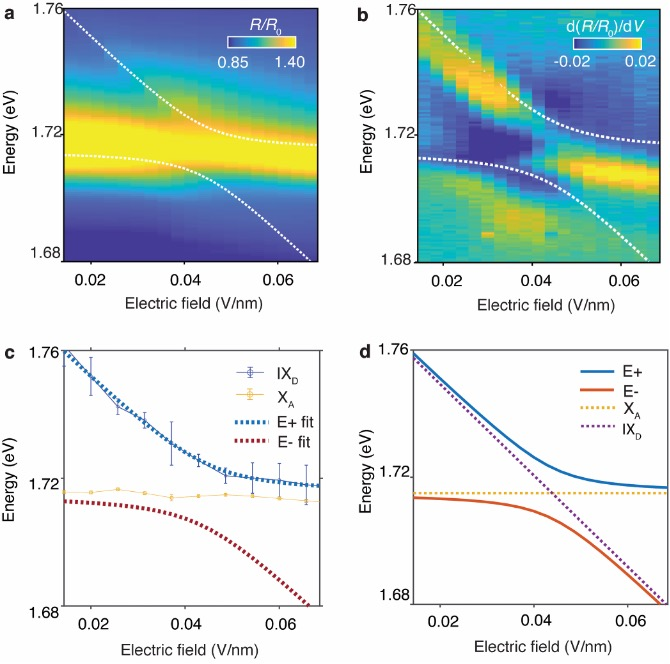
\includegraphics[width=0.8\textwidth]{Figures/C5/Fig5_3.jpg} % 
\end{center}
\caption[Analysis of anti-crossing between IX$_D$ and X$_A$ in device D1.] {\textbf{Analysis of anti-crossing between IX$_D$ and X$_A$ in device D1.} 
\textbf{a}, Reflectance spectra ($R/R_{0}$) as a function of the electric field near the anti-crossing region.  
\textbf{b}, Voltage derivative of reflectance spectra, $d(R/R_{0})/dV$.  
The white dashed lines in \textbf{(a)} and \textbf{(b)} represent the energies fitted with a two-level model.  
\textbf{c}, Fitted anti-crossing between the IX$_D$ and X$_A$.  
The solid lines with error bars in \textbf{(c)} denote the fitted peak energies of IX$_D$ (blue) and X$_A$ (yellow) extracted with Lorentzian fits to the spectra.  
The dotted line shows the IX$_D$ branch obtained from the coupled oscillator model.  
Error bars represent the variance of the fitted peak energies.  
\textbf{d}, Simulated two-level anti-crossing.}
\label{fig.5.3}
\end{figure}
\end{quote}
\renewcommand{\baselinestretch}{2}
\small\normalsize
% %///////////////////////
To quantitatively understand the avoided crossing, we extract the exciton energies by fitting reflectance spectra and then model the anti-crossing based on a two-level system with a Hamiltonian:
\begin{equation}
H =
\begin{pmatrix}
E_{1} & W \\
W & E_{2}
\end{pmatrix}
\label{eq:Hamiltonian}
\end{equation}
where $E_{1}$ and $E_{2}$ are the unperturbed energies of the IX$_{D}$ and X$_{A}$, respectively, and $W$ is the coupling strength. The new eigenvalues can be expressed as:
\begin{equation}
E_{\pm} = \frac{1}{2}(E_{1}+E_{2})
\pm \frac{1}{2}\sqrt{(E_{1}-E_{2})^{2}+4\lvert W\rvert^{2}}
\label{eq:eigenvalues}
\end{equation}
where $E_{\pm}$ correspond to the energies of the two branches.  
In Figures~\ref{fig.5.3}c, we extract the peak positions $E_{\pm}$ by fitting the reflectance spectra with Lorentzian functions.  
We then set $E_{2} = 1.715~\text{eV}$, corresponding to the mean energy of X$_A$, and keep it constant.  
$E_{1}$ is calculated based on the IX$_D$ energy at zero electric field and its Stark shift.  
The Stark shift slope $k$ is estimated to be $-1.436~\text{eV/V}$ for this device. 
The fitted anti-crossing is shown in Figures~\ref{fig.5.3}c,d, yielding a coupling parameter of $W = 10 \pm 2~\text{meV}$ between X$_A$ and IX$_D$. 

%////////////////////////////Figure Panel//////////////////
%Fig.5.4--------------
\renewcommand{\baselinestretch}{1}
\small\normalsize
\begin{quote}
\begin{figure}
\begin{center}
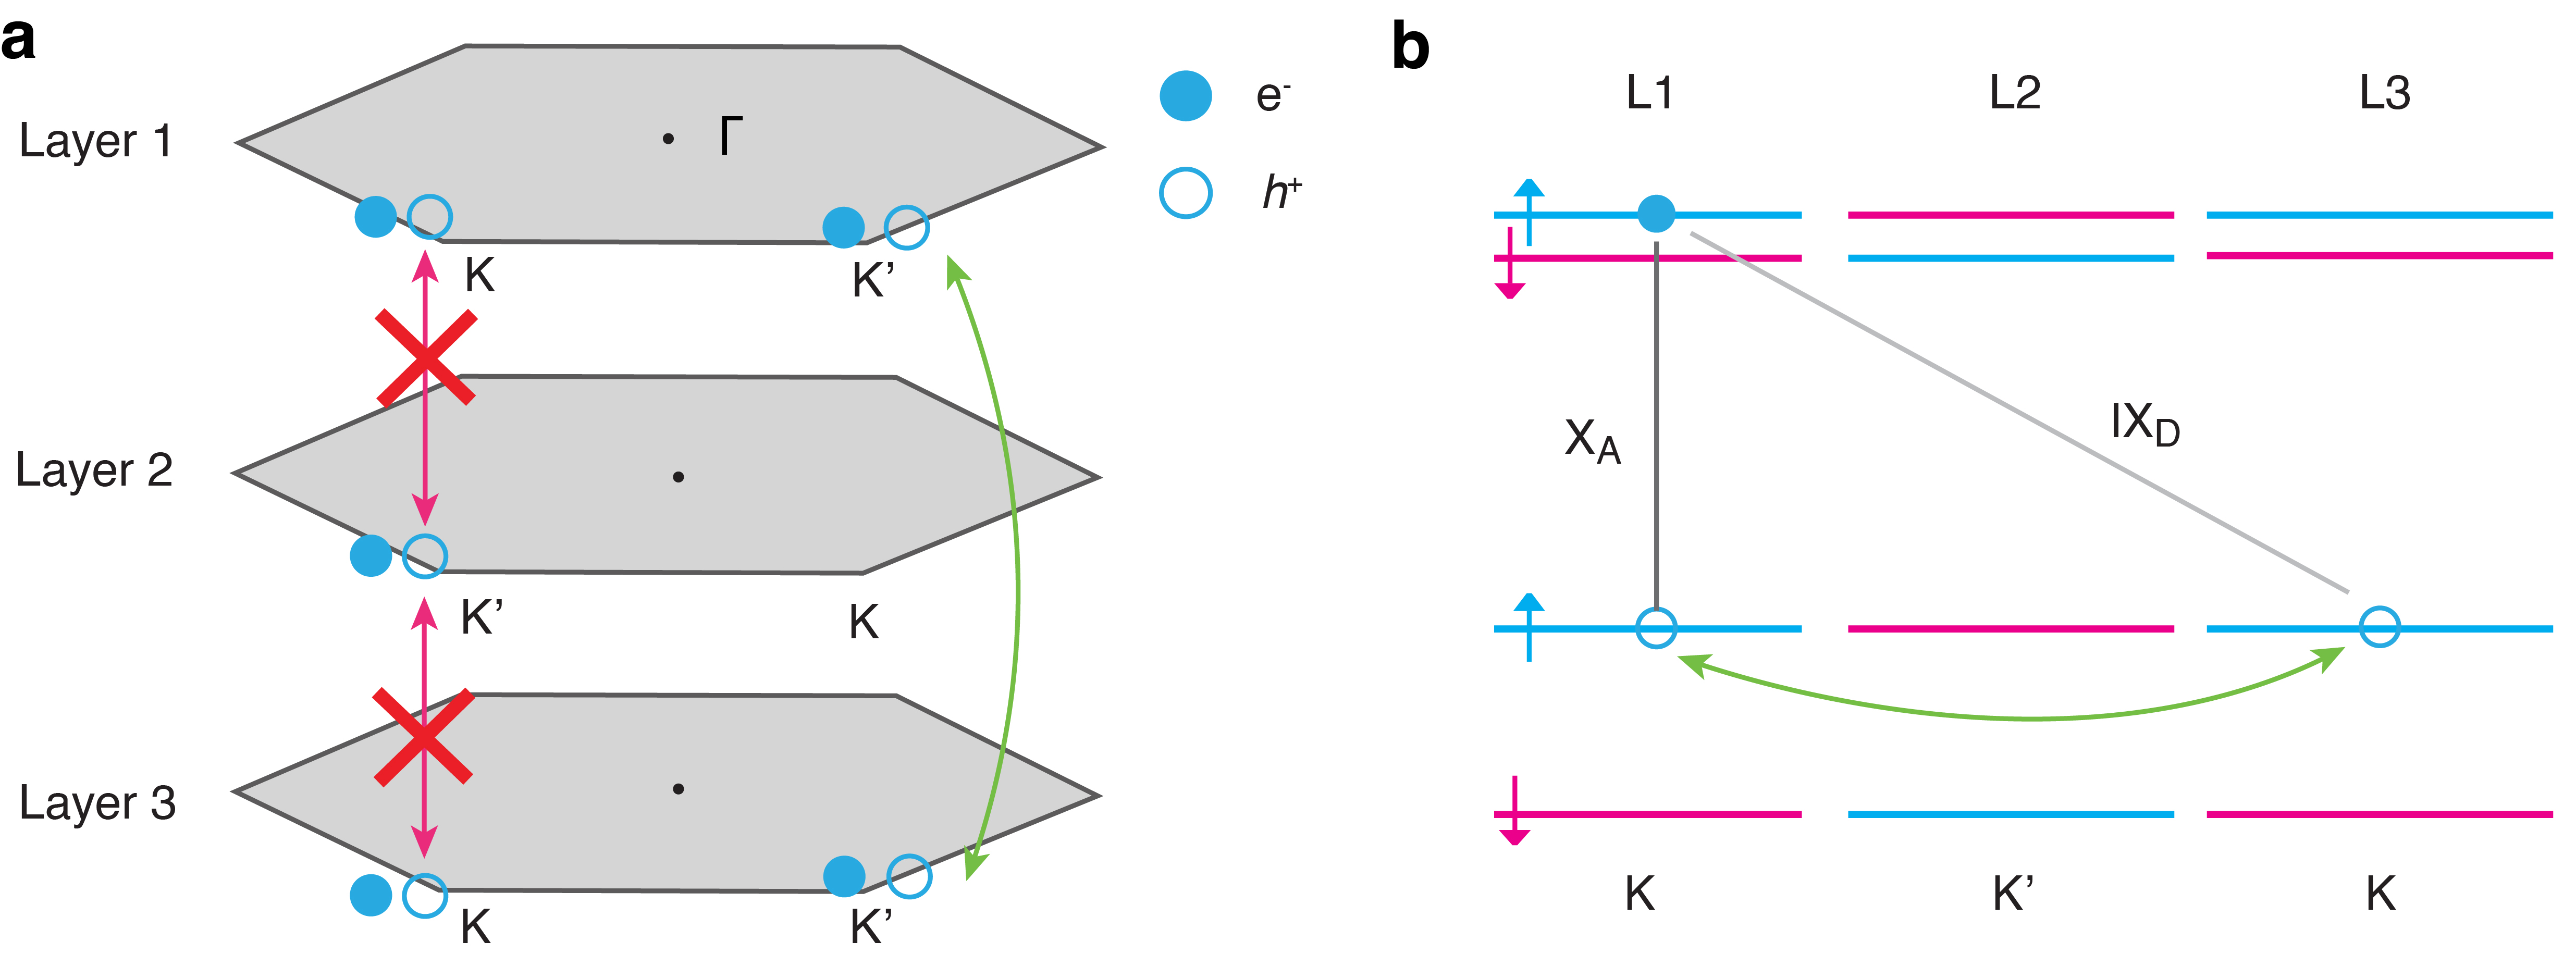
\includegraphics[width=0.9\textwidth]{Figures/C5/Fig5_4.jpg} % 
\end{center}
\caption[Electronic band structure of trilayer WSe$_2$.] 
{\textbf{Electronic band structure of trilayer WSe$_2$.} 
\textbf{a}, The crystal structure of natural trilayer WSe$_2$ dictates alternating $K$ and $K'$ valleys among neighboring layers.  
The strong spin--orbit coupling of holes leads to weak tunneling between neighboring layers but strong tunneling between the top and bottom layers.  
\textbf{b}, Hole tunneling between the top and bottom layers results in the hybridization of intralayer $K$--$K$ excitons X$_A$ and interlayer $K$--$K$ excitons IX$_D$. }
\label{fig.5.4}
\end{figure}
\end{quote}
\renewcommand{\baselinestretch}{2}
\small\normalsize
% %///////////////////////

The observed Stark effect and anti-crossing in WSe$_2$ trilayers can be understood by examining their crystal and band structure. 
In trilayers, each monolayer is rotated by $180^{\circ}$, resulting in alternating $K$ and $K'$ points between layers~\cite{ref27} (Figures~\ref{fig.5.4}a,b). 
Here we mainly consider the hole tunneling process, which is predicted to be much stronger than electron tunneling according to density functional theory calculations~\cite{ref28}. 
The sizeable spin--orbit coupling in the valence band dictates that direct tunneling between neighboring layers is much weaker than tunneling between the top and bottom layers across the middle layer (Figures~\ref{fig.5.4}a,b). 
Such tunneling gives rise to finite oscillator strength of interlayer $K$--$K$ excitons (IX$_D$) and their avoided crossing with intralayer excitons X$_A$~\cite{ref29}. 
Indeed, the experimentally extracted coupling strength between X$_A$ and IX$_D$ is consistent with the calculated interlayer hole tunneling strength at the $K$ valley~\cite{ref22}. 
This picture is further supported by our measured dipole moment of IX$_D$, which is close to the distance between the top and bottom layers, and it explains our observation that the level crossing at X$_A$ is not fully avoided, since IX$_D$ does not couple to intralayer excitons in the middle layer.

%////////////////////////////Figure Panel//////////////////
%Fig.5.5--------------
\renewcommand{\baselinestretch}{1}
\small\normalsize
\begin{quote}
\begin{figure}
\begin{center}
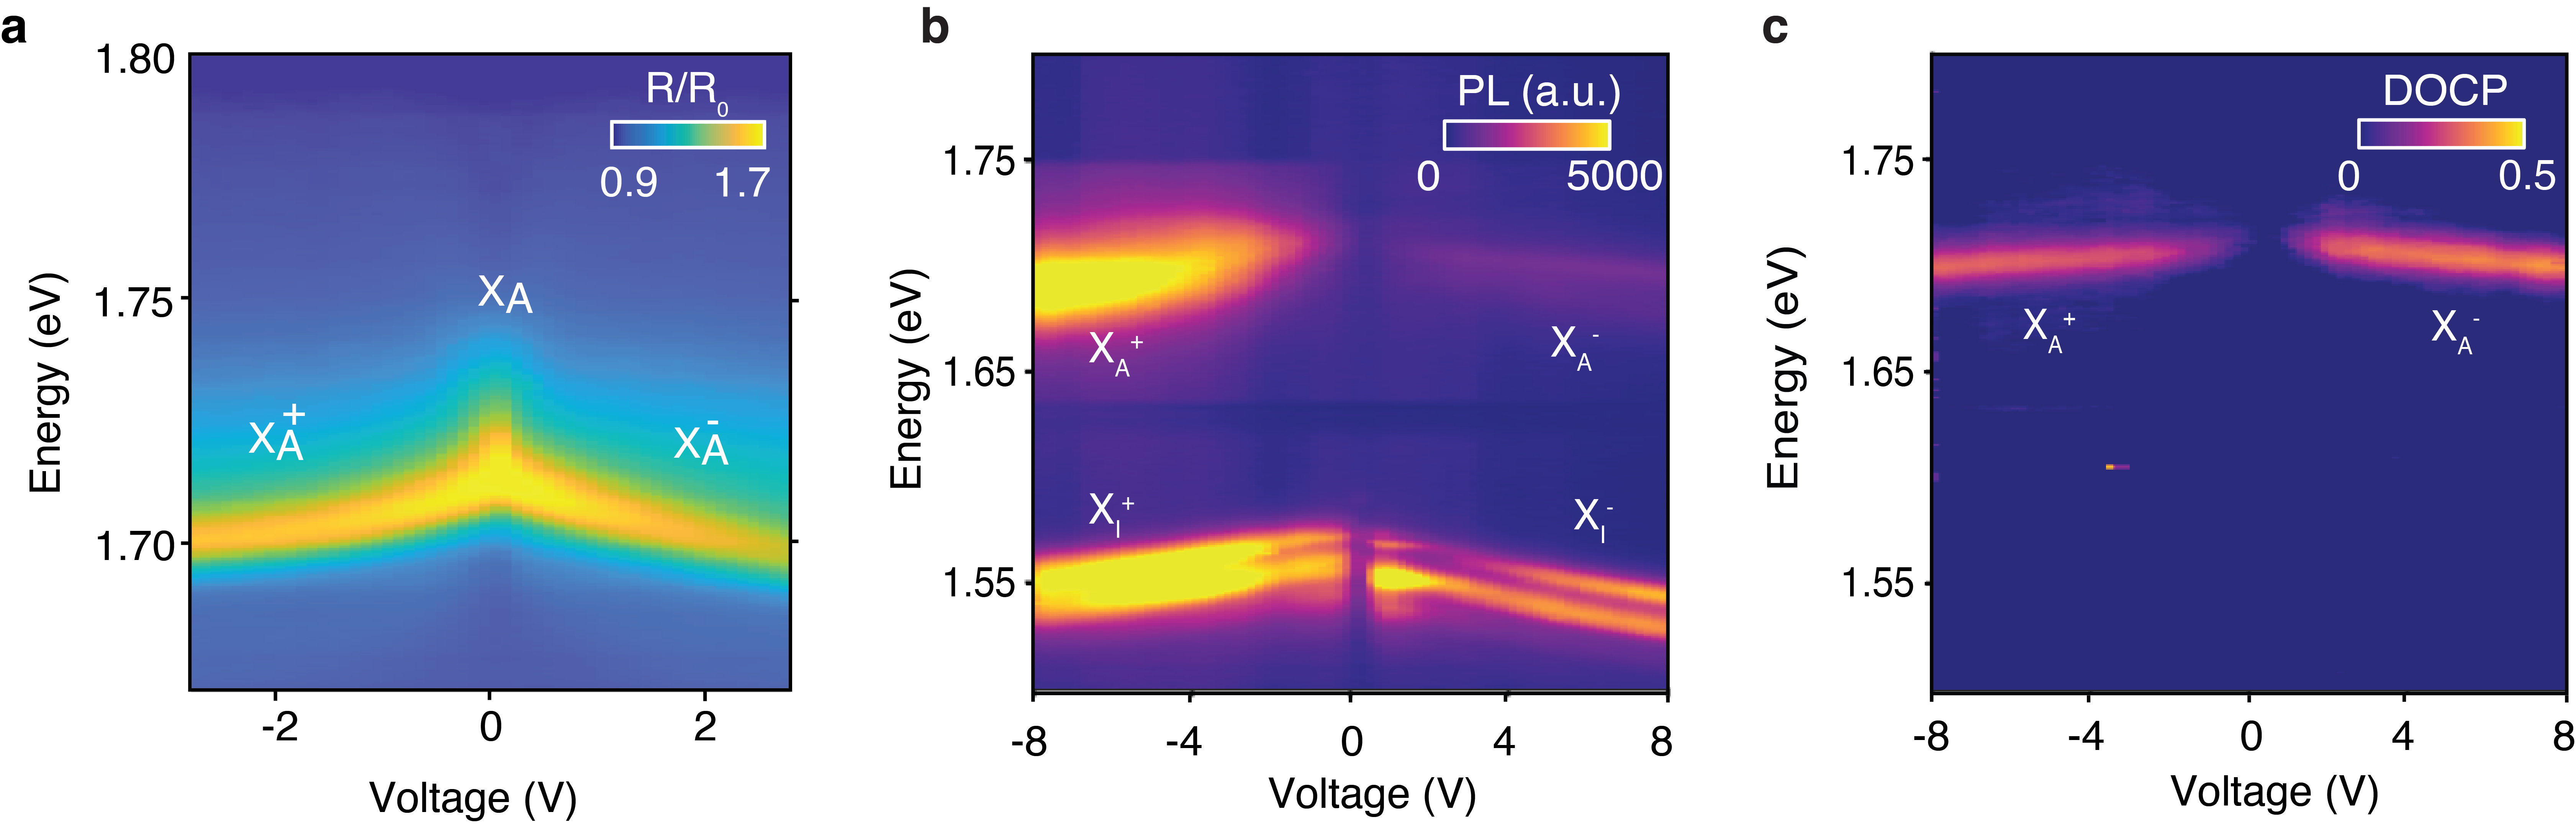
\includegraphics[width=1\textwidth]{Figures/C5/Fig5_5.jpg} % 
\end{center}
\caption[Doping-dependent optical characteristics of trilayer WSe$_2$ at 4~K.] 
{\textbf{Doping-dependent optical characteristics of trilayer WSe$_2$ at 4~K.} 
\textbf{a}, Doping-dependent reflectance spectra of the WSe$_2$ trilayer at 4~K, measured from device D1. 
With increasing doping concentration, the intralayer trion or Fermi polaron (X$_A^-$ / X$_A^+$) shifts toward lower energy.  
\textbf{b}, Doping-dependent photoluminescence of the trilayer WSe$_2$ at $E_z = 0$, measured from device D2 at 4~K under above-band excitation with a 635~nm diode laser.  
\textbf{c}, Degree of circular polarization (DOCP) of the X$_A^+$ and X$_A^-$. 
The bright emission in the range of 1.5--1.6~eV corresponds to the momentum-indirect trion/Fermi polaron, whereas the higher-energy emission around 1.7~eV corresponds to the momentum-direct ($K$--$K$) intralayer trion/Fermi polaron.  
Both charged excitons X$_I$ and X$_A$ exhibit a redshift with increasing doping density.  
}
\label{fig.5.5}
\end{figure}
\end{quote}
\renewcommand{\baselinestretch}{2}
\small\normalsize
% %///////////////////////
We further characterize how electrostatic gating modifies intralayer excitons X$_A$ and their hybridization with interlayer excitons. 
Figure~\ref{fig.5.5}a shows the doping-dependent reflectance spectra of the sample under zero electric field. 
Upon doping, the reflectance from neutral X$_A$ diminishes as they lose oscillator strength, while charged intralayer excitons emerge and shift to lower energies, with similar behavior observed in photoluminescence (PL) (Figure~\ref{fig.5.5}b). 
The redshift of charged excitons with increasing doping can be explained in terms of attractive Fermi polarons~\cite{ref23}, or by an increase in the exciton--trion energy splitting with increasing Fermi energy~\cite{ref24}. 
The similar doping dependence of reflectance and PL arises from the absence of Pauli blocking in both cases when the free carriers do not occupy the $K$ valley~\cite{ref25}. 
As we focus on the highly doped regime where excitons interact with a large number of carriers, we refer to these charged excitons as Fermi polarons in later discussions~\cite{ref23}.

\subsection{Giant optical nonlinearity of Fermi polaron}
Next, we study the nonlinear optical response of excitons by measuring the sample’s reflectance spectra under different laser pumping conditions.
Figures~\ref{fig.5.6}a--c show the reflectance spectra of the sample, probed with a halogen lamp, while being excited with a 635~nm continuous-wave (CW) laser of varying power. 
When the trilayers are electron-doped or intrinsic, optical pumping does not significantly alter the reflectance spectra. 
Intriguingly, however, in the hole-doped regime, optical pumping leads to a pronounced blueshift of the Fermi polaron X$_A^+$, on the order of a few meV, accompanied by a slight linewidth increase under tens of microwatts of excitation (Figure~\ref{fig.5.6}b). 
The oscillator strength of X$_A^+$, extracted from the reflectance spectra, remains nearly constant at low excitation power but decreases at higher power. 
We note that the PL signals are more than four orders of magnitude weaker than the reflected light and are therefore negligible.

%////////////////////////////Figure Panel//////////////////
%Fig.5.6--------------
\renewcommand{\baselinestretch}{1}
\small\normalsize
\begin{quote}
\begin{figure}
\begin{center}
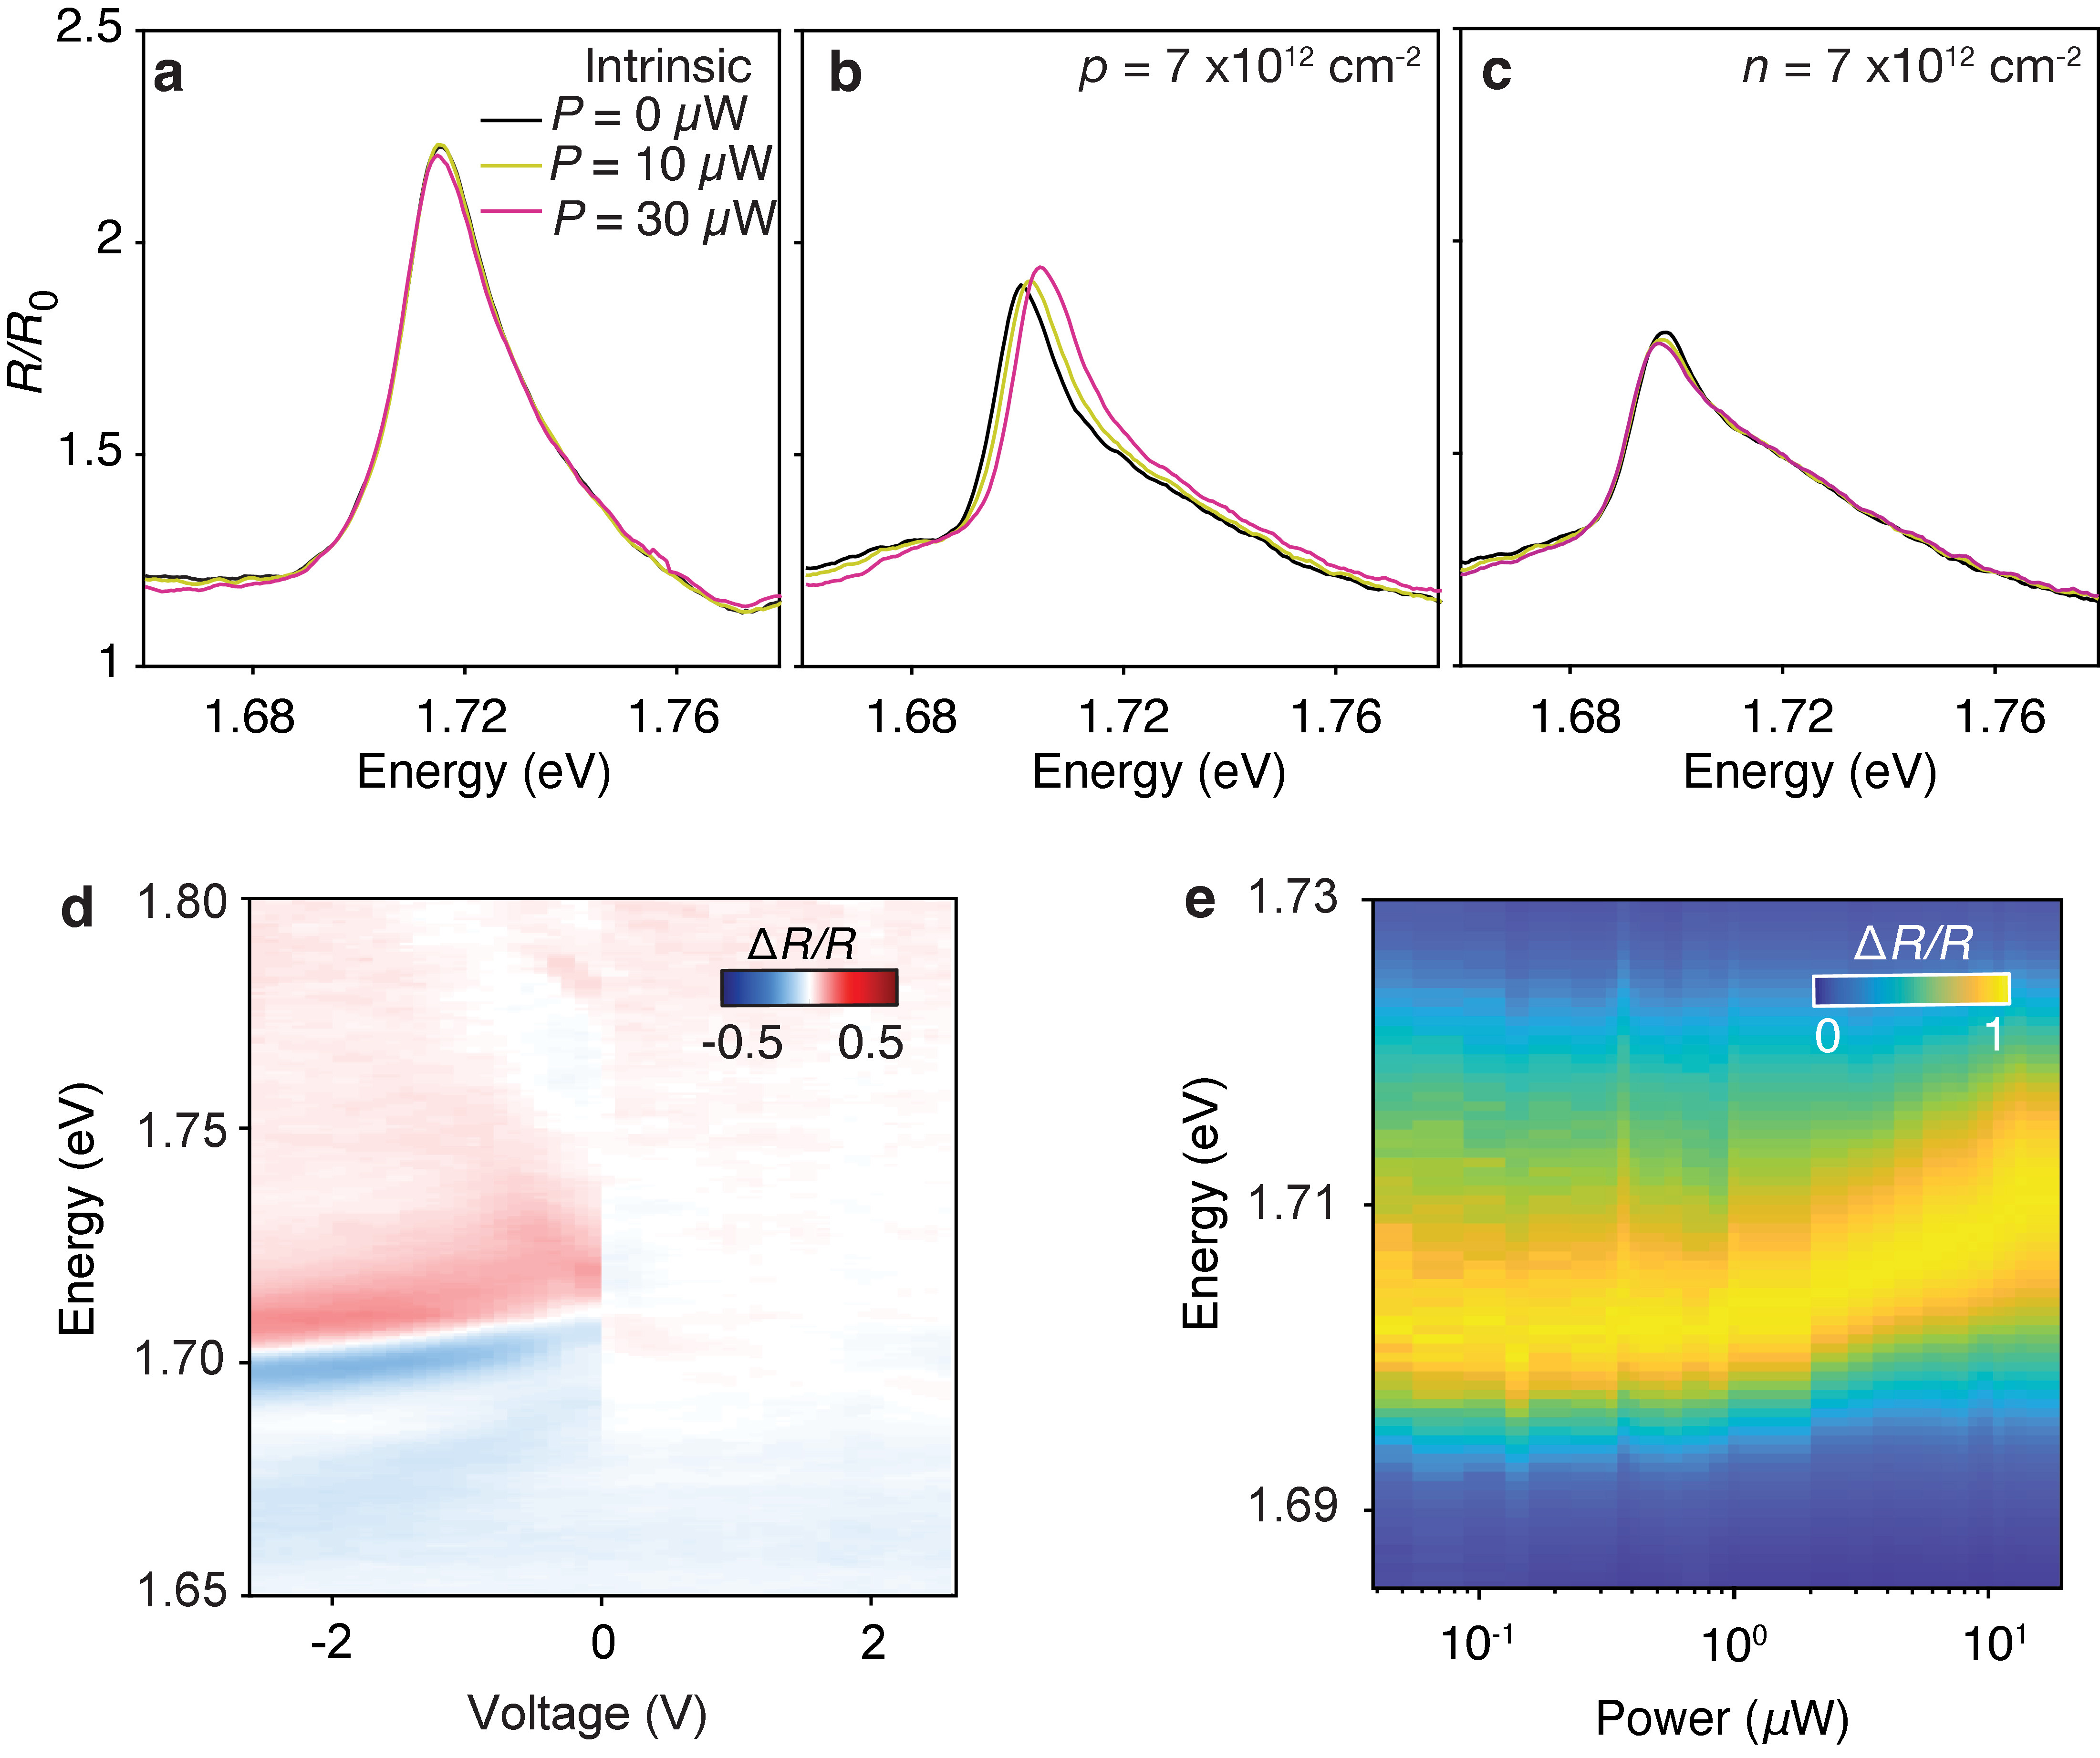
\includegraphics[width=0.85\textwidth]{Figures/C5/Fig5_6.jpg} % 
\end{center}
\caption[Nonlinearity in hole-doped homotrilayer WSe$_2$ at $T = 4$~K.] 
{\textbf{Nonlinearity in hole-doped homotrilayer WSe$_2$ at $T = 4$~K.} 
\textbf{a--c}, Reflectance contrast $R/R_{0}$ of the trilayer under 0~$\mu$W, 10~$\mu$W, and 30~$\mu$W CW (635~nm) laser excitation at different doping levels, where $R_{0}$ is the reflectance of a reference region near the trilayer (bare graphite/hBN/graphite on SiO$_2$). 
Intriguingly, the exciton blueshifts when the sample is hole-doped.  
\textbf{d}, Relative change in reflectance induced by 30~$\mu$W of CW laser pumping under different doping conditions. 
The color map is obtained by normalizing the reflectance with optical pumping to that without optical pumping,  
$\frac{\Delta R}{R} = \frac{R_{30\,\mu\mathrm{W}}}{R_{\mathrm{NoPump}}} - 1$.
Therefore,a positive value (red) at higher energies and a negative value (blue) at lower energies indicate a blueshift. 
The apparent discontinuity near 0~V is due to the high excitation power and finite voltage step used.  
\textbf{e}, Blueshift of X$_A^+$ as a function of pulsed laser excitation power (718--720~nm, resonant with X$_A^+$) at a hole density of $7 \times 10^{12}$~cm$^{-2}$. 
The apparent redshift in the peak energy below 1~$\mu$W is due to fluctuations; in fact, X$_A^+$ consistently shifts toward higher energy with increasing power.}
\label{fig.5.6}
\end{figure}
\end{quote}
\renewcommand{\baselinestretch}{2}
\small\normalsize
%////////////////////////////Figure Panel//////////////////

% To visualize the doping dependence of the nonlinearity, we measure the relative change in the sample’s reflectance induced by optical pumping,  
% $\frac{\Delta R}{R} = \frac{R_{p}}{R_{np}} - 1$,
% where $R_{p}$ and $R_{np}$ are the sample’s reflectance spectra with and without laser pumping, respectively. 
% Figure~5.6d shows $\Delta R / R$ under symmetric gating with zero electric field, where we observe a striking asymmetry between the electron- and hole-doped regimes. 
% We briefly note that the observed nonlinearity of intralayer excitons is orders of magnitude stronger than that of dipolar interlayer excitons in bilayer TMDs~\cite{ref19,ref26} (see Table~S1 for a detailed comparison with other systems). 
% Another critical distinction is that the nonlinearity in bilayer TMDs occurs for interlayer excitons in the intrinsic regime~\cite{ref1,ref19}.
%////////////////////////////Figure Panel//////////////////
%Fig.5.7--------------
\renewcommand{\baselinestretch}{1}
\small\normalsize
\begin{quote}
\begin{figure}
\begin{center}
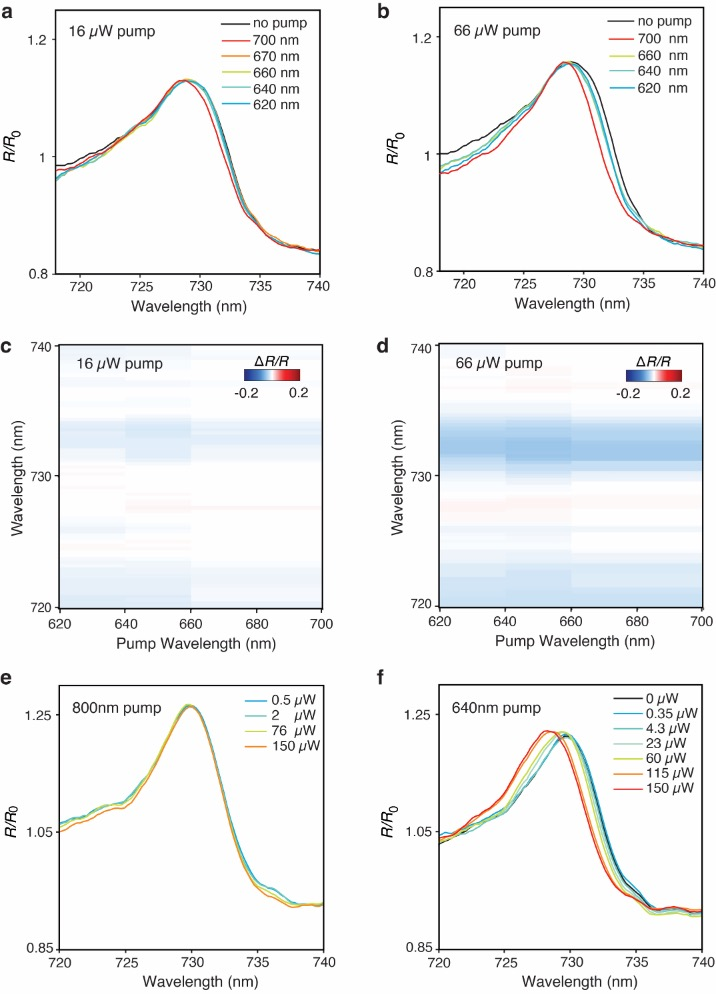
\includegraphics[width=0.7\textwidth]{Figures/C5/Fig5_7.jpg} % 
\end{center}
\caption[Effect of pumping photon energy on nonlinearity.] 
{\textbf{Effect of pumping photon energy on nonlinearity.}
\textbf{a, b,} Blueshift of X$_A^+$ under laser excitation at different center wavelengths ($\sim$10~nm spectral width) with a fixed pumping power at \textbf{(a)} 16~$\mu$W and \textbf{(b)} 66~$\mu$W. 
\textbf{c, d,} The corresponding reflectance changes induced by optical pumping at different wavelengths show no significant wavelength dependence. 
\textbf{e, f,} when exciting the system with photon energies below X$_A^+$, we did not observe significant blueshift \textbf{(e)}, in contrast to higher energy excitation at 640~nm \textbf{(f)}. 
All data is acquired from device D3. We also note that the resonant excitation results in a much more pronounced blueshift.
}
\label{fig.5.7}
\end{figure}
\end{quote}
\renewcommand{\baselinestretch}{2}
\small\normalsize
% %///////////////////////

To visualize the doping dependence of the nonlinearity, we measure the relative change in the sample’s reflectance induced by optical pumping,  
$\frac{\Delta R}{R} = \frac{R_{p}}{R_{np}} - 1$,
where $R_{p}$ and $R_{np}$ are the sample’s reflectance spectra with and without laser pumping, respectively. 
Figure~5.6d shows $\Delta R / R$ under symmetric gating with zero electric field, where we observe a striking asymmetry between the electron- and hole-doped regimes. 
We briefly note that the observed nonlinearity of intralayer excitons is orders of magnitude stronger than that of dipolar interlayer excitons in bilayer TMDs~\cite{ref19,ref26} (see Table~S1 for a detailed comparison with other systems). 
Another critical distinction is that the nonlinearity in bilayer TMDs occurs for interlayer excitons in the intrinsic regime~\cite{ref1,ref19}.

In addition to non-resonant excitation, we also probe the optical nonlinearity by resonantly exciting X$_A$ with a pulsed laser (718--730~nm wavelength, $\sim$100~ps pulse duration), and we observe qualitatively similar nonlinear behavior with a $\sim$10~meV blueshift of X$_A^+$ and a linewidth increase, but only on the hole-doped side(Figure~\ref{fig.5.6}e). 
To investigate how excitation photon energy impacts the nonlinearity, we tune the pulsed laser energy across the X$_A^+$ resonance. 
This resonant excitation results in a stronger blueshift than higher-energy excitation, while no obvious shift in X$_A^+$ is observed when the photon energy falls below X$_A^+$ (Figure~\ref{fig.5.7}). 
Additionally, we find no significant wavelength dependence when the photon energy exceeds X$_A^+$ (Figure~\ref{fig.5.7}). 
Notably, pulsed excitation generates an order-of-magnitude smaller blueshift than the CW laser at lower power, even though its peak power is comparable to the CW laser’s average power (Figure~\ref{fig.5.8}).

%////////////////////////////Figure Panel//////////////////
%Fig.5.8--------------
\renewcommand{\baselinestretch}{1}
\small\normalsize
\begin{quote}
\begin{figure}
\begin{center}
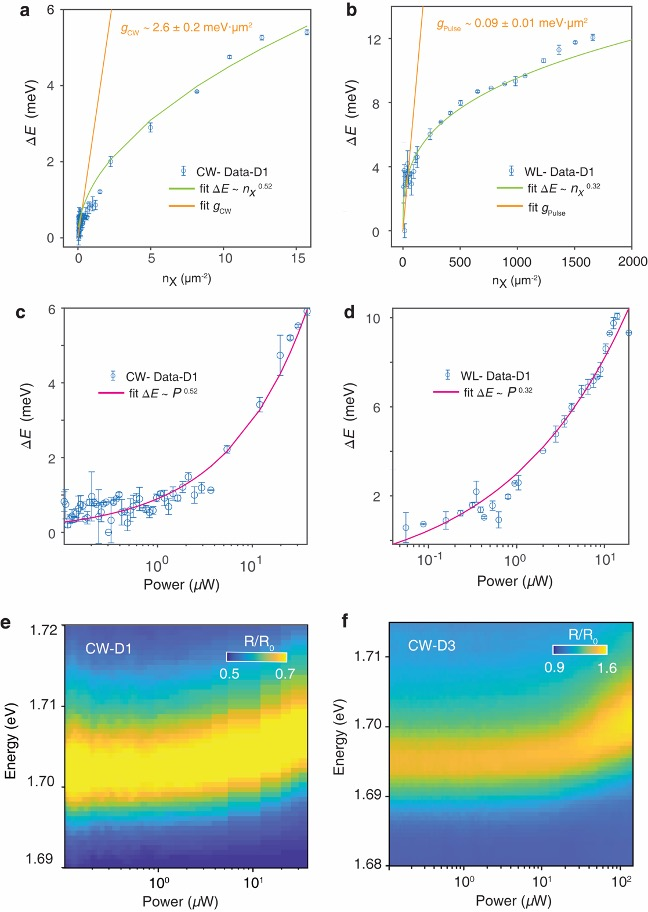
\includegraphics[width=0.75\textwidth]{Figures/C5/Fig5_8.jpg} % 
\end{center}
\caption[Analysis of power-dependent blueshift of X$_A^+$ under CW laser (a, c) and white laser excitation (b, d).] 
{\textbf{Analysis of power-dependent blueshift of X$_A^+$ under CW laser (a, c) and white laser excitation (b, d).}
\textbf{a,b,} Extraction of interaction strength $g$ from \textbf{(a)} CW laser and \textbf{(b)} pulsed laser pumping induced X$_A^+$ blueshift vs. exciton density for D1. 
The exciton density is calculated from pump flux based on $n_X=P \alpha \tau/\hbar \omega$, where $P$ is the pump power, $\alpha$ is the absorption coefficient, $\tau$ is the lifetime of the Fermi polaron, $\hbar \omega$ is the photon energy. 
The Fermi polaron lifetime is assumed as 2 ps. 
The interaction strength is extracted from the linear fit of the $\Delta E$--$n_X$ curve in the low exciton density regime. 
The larger $g$ values under CW excitation could be related to the complex relaxation dynamics of the exciton populations and an overestimation of exciton density under pulsed excitation. 
We also fit the blue shift amount as $\Delta E = a \cdot n_X^{(b)}$ over the entire data range. 
The fitting for CW laser and pulsed laser shows a sublinear response for X$_A^+$ as polaron density. 
The hole doping density is kept at $8 \times 10^{12}$ cm$^{-2}$. 
\textbf{c, d,} The same data as shown in \textbf{a, b,} plotted on semilog scale, with power as the x-axis. 
\textbf{e, f,} Power-dependent blueshift of X$_A^+$ under CW laser for \textbf{e,} device D1 and \textbf{f,} device D3. 
All error bars in \textbf{a-d} represent the variance of fitting peak energy.
}
\label{fig.5.8}
\end{figure}
\end{quote}
\renewcommand{\baselinestretch}{2}
\small\normalsize
% %///////////////////////
%////////////////////////////Figure Panel//////////////////
%Fig.5.9--------------
\renewcommand{\baselinestretch}{1}
\small\normalsize
\begin{quote}
\begin{figure}
\begin{center}
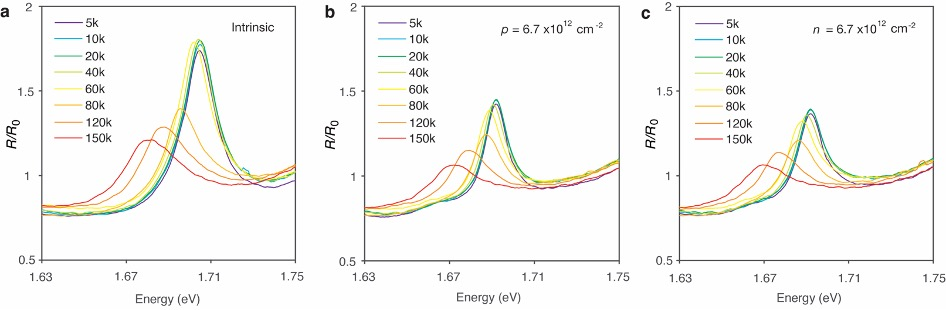
\includegraphics[width=1\textwidth]{Figures/C5/Fig5_9.jpg} % 
\end{center}
\caption[Temperature-dependent reflectance spectra of the trilayer under a constant doping density under zero electric field.] 
{\textbf{Temperature-dependent reflectance spectra of the trilayer under a constant doping density under zero electric field.}
In all cases, which include \textbf{(a)} intrinsic, \textbf{(b)} hole-doping, and \textbf{(c)} electron-doping, we observe strong redshift with increasing temperatures. Therefore, the observed nonlinearity, which corresponds to exciton blueshift, cannot be described as simple laser heating effects.}
\label{fig.5.9}
\end{figure}
\end{quote}
\renewcommand{\baselinestretch}{2}
\small\normalsize
% %///////////////////////

\section{Discussions}
The observed optical nonlinearity and their doping dependence cannot be simply explained by heating or carrier injection from the laser since both effects result in redshift of the intralayer excitons (Figures~\ref{fig.5.5}a and~\ref{fig.5.9}). 
Therefore, we examine how the interactions among the elementary excitations in the systems, \textit{i.e.}, intralayer excitons X$_A$, momentum-indirect excitons X$_I$, and free carriers, may give rise to the observed nonlinearity.

\subsection{Estimation of exciton interaction strength}
First, we extract a large interaction strength $g \sim 2~\mathrm{meV}\,\mu\mathrm{m}^{2}$ from the linear fit of energy blueshift vs.\ X$_A^+$ density at low power~\cite{ref30} (Figure~\ref{fig.5.8}). 
It is apparent that excitonic interactions (i.e.\ between X$_A$--X$_A$ and X$_A$--X$_I$) alone cannot produce the observed nonlinearity. 
On the one hand, the X$_A$--X$_A$ interactions among intralayer excitons are repulsive but weak, which scales linearly with density with a coefficient of $g_{\mathrm{ex}}\sim \alpha E_B R^{2}\sim 1.9~\mu\mathrm{eV}\,\mu\mathrm{m}^{2}$, where $\alpha$ is a constant ($\sim 6$), $E_B \approx 100~\mathrm{meV}$ is the exciton binding energy and $R$ ($\sim 1.78~\mathrm{nm}$) denotes the exciton Bohr radius in trilayers~\cite{ref31}. 
Given the short lifetime of X$_A$ ($\sim$picoseconds)~\cite{ref32,ref33} and thus the small density ($\sim 10^{9}~\mathrm{cm}^{-2}$), the amount of blueshift is expected to be orders of magnitude smaller than the experimental values (and comparable to monolayers and bilayers~\cite{ref20,ref31}). 
On the other hand, although X$_A$ can acquire a dipole moment via its hybridization with IX$_D$ and experience X$_A$--X$_I$ dipolar interaction with X$_I$, such interactions should have persisted in the intrinsic and electron-doped regime. 
Furthermore, we estimate an upper limit of dipolar interaction strength. 
We note that to the first order, there should be zero net dipoles and weak dipolar interactions under symmetric gating. 
However, the emergence of local net dipoles is plausible due to spontaneous symmetry breaking. 
Considering this, we calculate an upper limit for the dipolar interactions, assuming all dipoles are aligned. 
Using a parallel plate model, the dipolar interaction strength is given by $g_d=\frac{e^{2} d}{\varepsilon_{0}\,\varepsilon_{\mathrm{TMD}}}$, where $e d$ is the dipole moment of X$_A$. 
This dipole moment, $e d$, acquired from the hybridization with IX$_D$, can be estimated from the composition percentage of each exciton species in the coupled oscillator model. 
The value peaks when X$_A$ become degenerate with IX$_D$ reaching $\sim 0.7~\mathrm{nm}\cdot e$, and leading to an estimated dipolar interaction strength of $g_d \sim 1.8~\mu\mathrm{eV}\,\mu\mathrm{m}^{2}$, orders of magnitude smaller than the experimental interaction strength $g$. 
This conclusion is supported by the experimental observation of much weaker nonlinearity of X$_I$ than X$_A^+$, even when X$_I$ is fully polarized by an external electric field (see Figure~\ref{fig.5.10}).

%////////////////////////////Figure Panel//////////////////
%Fig.5.10--------------
\renewcommand{\baselinestretch}{1}
\small\normalsize
\begin{quote}
\begin{figure}
\begin{center}
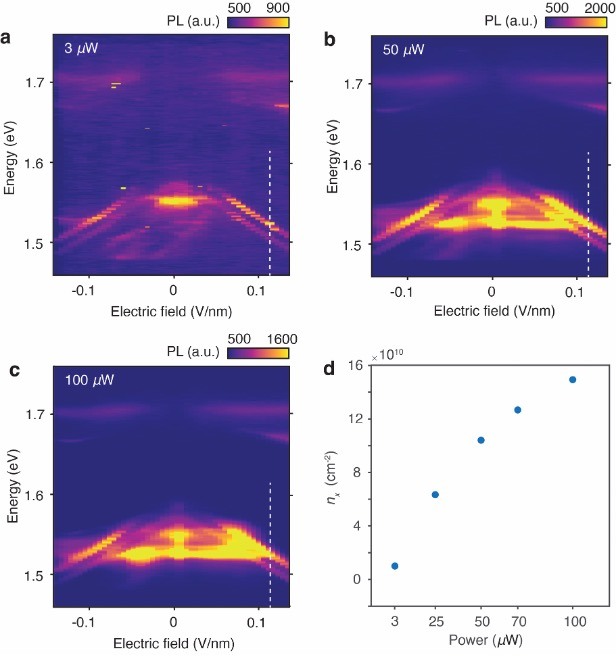
\includegraphics[width=0.75\textwidth]{Figures/C5/Fig5_10.jpg} % 
\end{center}
\caption[Estimation of X$_I$ density as a function of pump power.] 
{\textbf{Estimation of X$_I$ density as a function of pump power.}
\textbf{a-c,} Electric field-dependent PL map under different pump power \textbf{(a)} 3 $\mu$W, \textbf{(b)} 50 $\mu$W, \textbf{(c)} 100 $\mu$W at the trilayer region. 
At an electric field of 0.12 V/nm, a maximum blue shift in a value of 3.3 meV of the X$_I$ is observed. 
\textbf{(f)} X$_I$ exciton density inferred from the above X$_I$ blueshift under an applied electric field of 0.12 V/nm.
}
\label{fig.5.10}
\end{figure}
\end{quote}
\renewcommand{\baselinestretch}{2}
\small\normalsize
% %///////////////////////

\subsection{Nonlinearity due to valley polarization}
Therefore, we attribute the observed nonlinearity to a valley polarization created from the interactions between X$_A$ and free carriers. 
In particular, excitons created by optical pumping may induce a nonequilibrium valley population imbalance of resident carriers between $K$ and $\Gamma$ valleys, via mechanisms such as exciton--carrier scattering~\cite{ref34,ref35}. 
Importantly, under zero electric field, the energy difference between $K$ and $\Gamma$ valleys is rather small in trilayers~\cite{ref22}, on the order of tens of millielectronvolts, based on first-principle calculations and transport studies (Figure~\ref{fig.5.11}a). 
As a result, electrostatically doped holes at the $\Gamma$ point could be efficiently scattered into the $K$ valley by excitons such as X$_A$ and X$_I$, via Coulombic and exchange interactions~\cite{ref34,ref35} (Figure~\ref{fig.5.11}b). 
This net accumulation of valley population at $K$ (and $K'$) induces phase-space filling and, consequently, the observed blueshift of X$_A^+$. 
Such a scattering process would also introduce additional dephasing, which explains the increase in the X$_A^+$ linewidth.

%////////////////////////////Figure Panel//////////////////
%Fig.5.11--------------
\renewcommand{\baselinestretch}{1}
\small\normalsize
\begin{quote}
\begin{figure}
\begin{center}
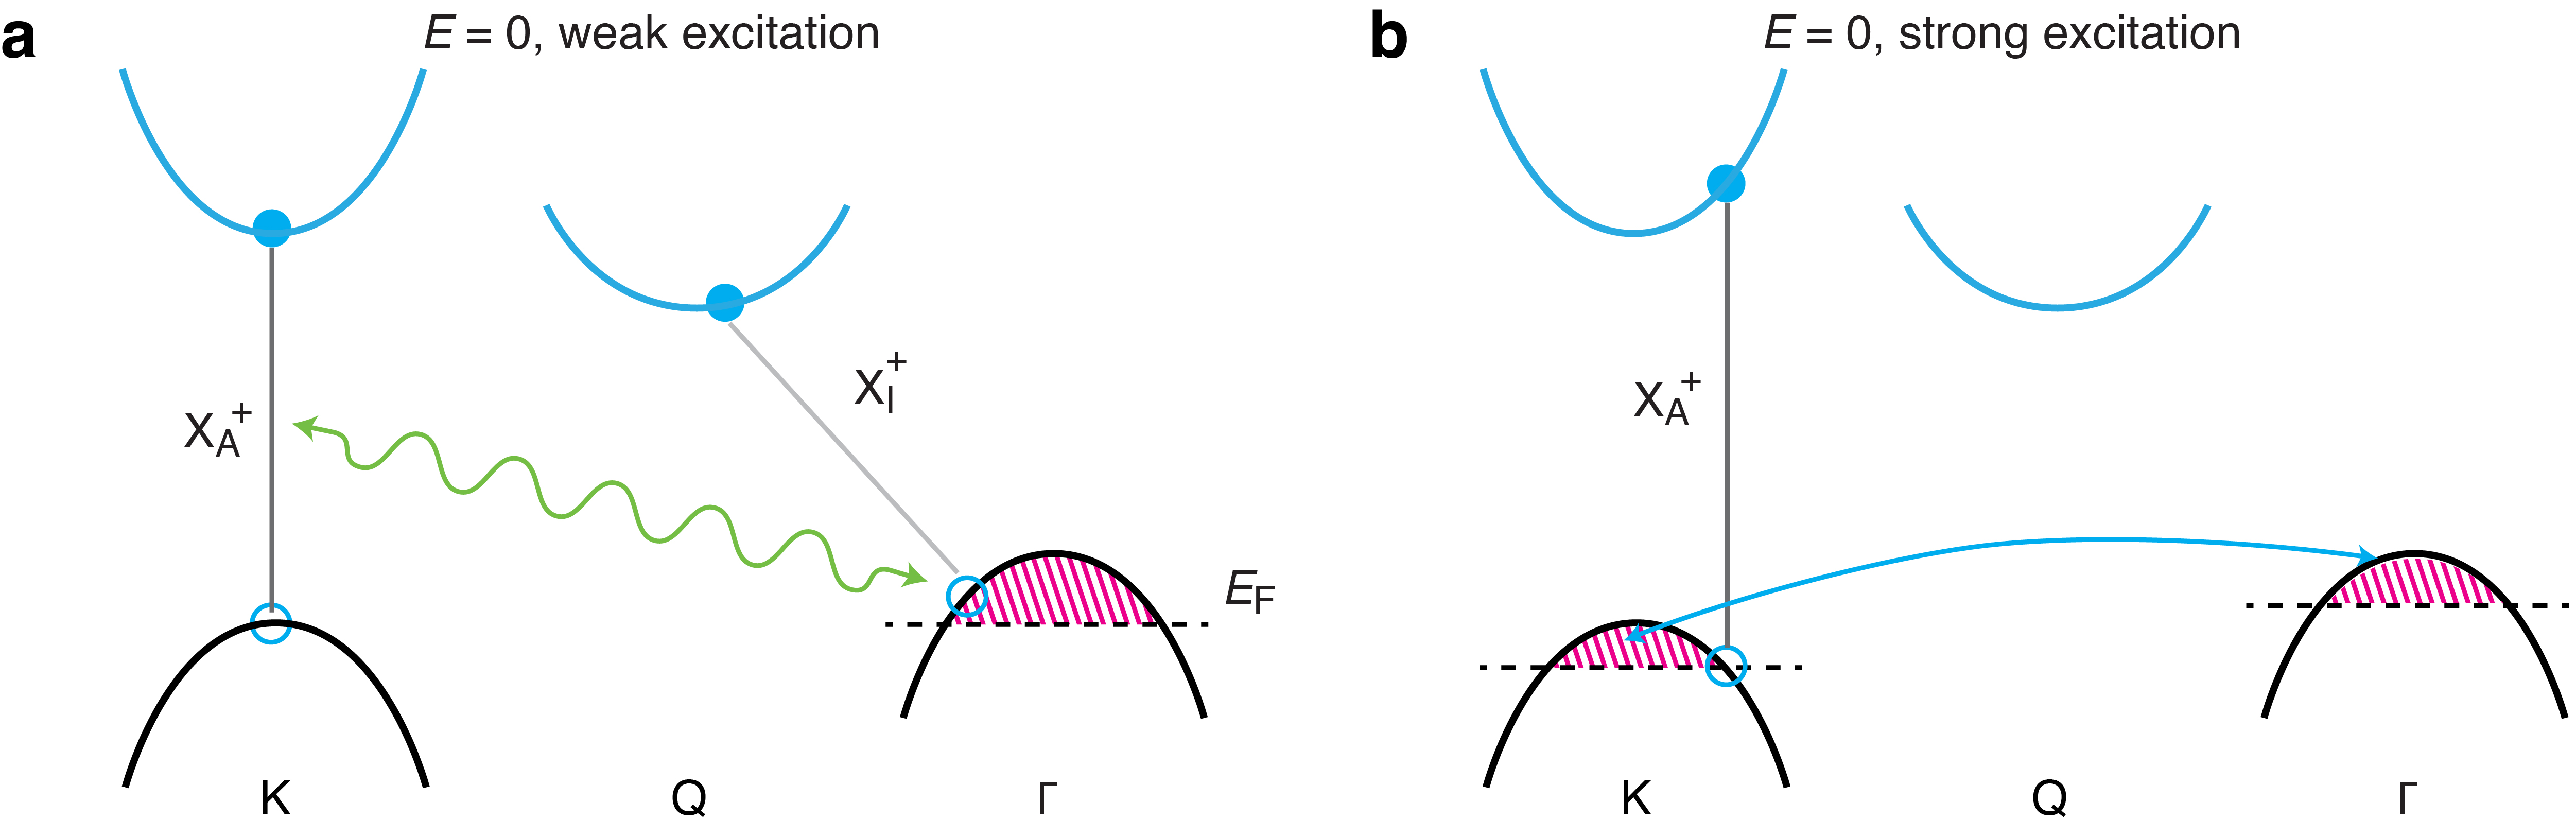
\includegraphics[width=1\textwidth]{Figures/C5/Fig5_11.jpg} % 
\end{center}
\caption[Optically induced valley polarization.] 
{\textbf{Optically induced valley polarization.}
\textbf{a, }Optical excitation generates both momentum direct intralayer X$_A^+$  and momentum indirect XI of higher population. 
Intralayer Fermi polaron X$_A^+$ can interact with X$_I$ and the free holes in the system. 
\textbf{b,} Under strong optical excitation, the interaction between intralayer excitons and free charges can induce a population transfer of carriers from the $\Gamma$ to the $K$ valley. 
The energy difference between $\Gamma$ and $K$ is small. 
The additional free carriers in K valley leads to phase space filling and optically induced blueshift of X$_A^+$. We note that in this nonequilibrium state, the dashed lines do not represent the Fermi level but are indications for the carrier population.
}
\label{fig.5.11}
\end{figure}
\end{quote}
\renewcommand{\baselinestretch}{2}
\small\normalsize
% %///////////////////////
Meanwhile, the oscillator strength remains unchanged at low excitation power, since it depends on the total doping level, but decreases at higher power due to saturation. 
In addition to the exciton--carrier scattering, the net valley polarization may also be created by the electric field induced by optical pumping. 
For instance, it has been suggested in bilayer TMDs that the generation of dipolar X$_I$ excitons may create a non-zero displacement field due to spontaneous symmetry breaking~\cite{ref1}. 
Such a displacement field can introduce a relative energy shift between $K$ and $\Gamma$ valleys~\cite{ref22}, thus creating a valley polarization. 
To further investigate such possible valley polarization, we probe the population of the resident carriers in the $K$ and $K'$ valleys under circularly polarized resonant excitation. 
As shown in Figure~\ref{fig.5.12}, we observe a stronger blueshift of X$_A^+$ in the $K$ than in the $K'$ valley when exciting excitons in the $K$ valley, consistent with our optically induced valley polarization picture.

%////////////////////////////Figure Panel//////////////////
%Fig.5.12--------------
\renewcommand{\baselinestretch}{1}
\small\normalsize
\begin{quote}
\begin{figure}
\begin{center}
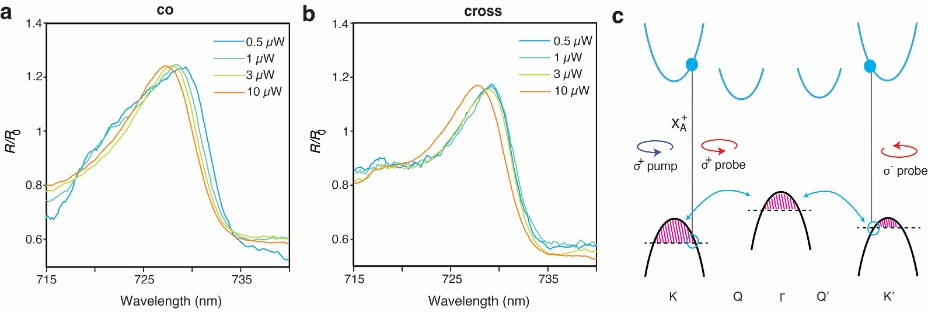
\includegraphics[width=1\textwidth]{Figures/C5/Fig5_12.jpg} % 
\end{center}
\caption[Valley-polarized holes under resonant circularly polarized excitation.] 
{\textbf{Valley-polarized holes under resonant circularly polarized excitation.} \textbf{a, b,} Power-dependent blueshift of X$_A^+$ under resonant pumping with \textbf{(a)} $\sigma^+/\sigma^+$ (pumping and probing $K$ valley) and \textbf{(b)} $\sigma^+/\sigma^-$ configuration (pumping $K$, while probing $K'$ valley) when the sample is hole-doped. 
We observe a stronger blueshift of X$_A^+$ in \textbf{(a)}. 
In particular, we observe a $\sim$1.3~nm blueshift under 3~$\mu$W pump when the pump and probe are co-polarized and no obvious shift in the cross-polarized case. 
Further increasing the pumping power to 10~$\mu$W leads to a blueshift in the cross-polarized setup, albeit still being smaller than the co-polarized case, which suggests the holes are partially polarized in $K$ vs.\ $K'$. 
The data is acquired from device D3. 
\textbf{c,} Nonequilibrium hole accumulation in $K$ and $K'$ valleys induced by selective valley pumping with a circularly polarized excitation. 
The resulting population imbalance between $K$ and $K'$ causes different amounts of blueshift in X$_A^+$ nonlinearity between the two valleys.   
}
\label{fig.5.12}
\end{figure}
\end{quote}
\renewcommand{\baselinestretch}{2}
\small\normalsize
% %///////////////////////
The proposed valley polarization mechanism also explains the strong electron--hole asymmetry of optical nonlinearity. 
Intrinsic trilayer WSe$_2$ exhibit weak nonlinearity, since no valley polarization can be created without resident carriers. 
In the electron-doped case, the valley polarization of resident carriers is prevented by the much larger energy splitting, on the order of hundreds of millielectronvolts, between $Q$ (band minimum) and the $K$ valleys (where X$_A$ resides) in the conduction band~\cite{ref22}. 
We also briefly note that in TMD monolayers, optical pumping with circularly polarized light can polarize carriers in $K$ vs.\ $K'$ valleys~\cite{ref32,ref33,ref34,ref35,ref36,ref37,ref38}. 
The generation of valley imbalance in monolayers has been attributed to mechanisms such as different inter-valley vs.\ intra-valley carrier relaxation rates, and different indirect excitons and spin-forbidden dark excitons relaxation rates~\cite{ref39,ref40}. 
Unlike in monolayers, where a spin flip of carriers is required for scattering between $K$ and $K'$ valleys, the $\Gamma$ point is spin-degenerate so that the intervalley scattering between $K$ and $\Gamma$ in trilayers can happen via a spin-conserving process, such as direct Coulomb and exchange interactions between holes and excitons. 
We note that X$_I$ likely plays a crucial role in exciton--electron scattering owing to their larger population than X$_A$ (see Figure~\ref{fig.5.10} for estimated X$_I$ density). 
Since relaxation processes of X$_A \rightarrow$ X$_I$ and X$_I \rightarrow$ ground state both involve finite momentum transfer, they can facilitate the valley polarization process via exciton--carrier scattering. 
This suggests that the dynamics of valley polarization could occur at a timescale similar to the X$_I$ lifetime, on the order of nanoseconds, which may explain our observation of weaker nonlinearity created by the pulsed laser compared to CW excitation with the same peak power (Figure~\ref{fig.5.8}).

To further corroborate our hypothesis, we control the relative energies of $\Gamma$ and $K$ valleys by applying an external electric field~\cite{ref20,ref22}, and study the resulting changes in both the energies and optical nonlinearity of Fermi polarons. 

First, we measure the reflectance of the X$_A^+$ and X$_A^-$ as we change the electric field under fixed doping levels (Figures~\ref{fig.5.13}a,b). 
With an increasing field, the energy of the X$_A^+$ blueshifts at a smaller electric field and then switches to a redshift above an electric field of $\sim$0.05~V/nm (Figure~\ref{fig.5.13}a). 
The electric field shifts the valence band maximum from $\Gamma$ to $K$ due to the distinct orbital characters of the eigenstates~\cite{ref22}. 
While the eigenstate at $K$ becomes layer-polarized with higher energies with the field, the wavefunction at the $\Gamma$ point features large interlayer coupling with only small energy changes under the field~\cite{ref22}.
This shift from $\Gamma$ to $K$ leads to more phase-space filling in $K$ and a blueshift of X$_A^+$, consistent with our proposed mechanism for optical nonlinearity (Figure~\ref{fig.5.14}). 
Above an electric field of $\sim$0.05~V/nm, X$_A^+$ begins to redshift. 
This electric field is comparable to the critical field under which the band edge shifts from $\Gamma$ to $K$, as determined from transport studies~\cite{ref22} (note that the literature-reported field differs from our definition by a factor of the relative dielectric constant). 

In stark contrast, the energy shift of the X$_A^-$ is much smaller in the electron-doped region (Figure~\ref{fig.5.13}b), where the band edge remains at the $Q$ point. 
The small energy variation of X$_A^-$ can be explained by the avoided crossing, similar to the undoped case.

%////////////////////////////Figure Panel//////////////////
%Fig.5.13--------------
\renewcommand{\baselinestretch}{1}
\small\normalsize
\begin{quote}
\begin{figure}[htbp]
\begin{center}
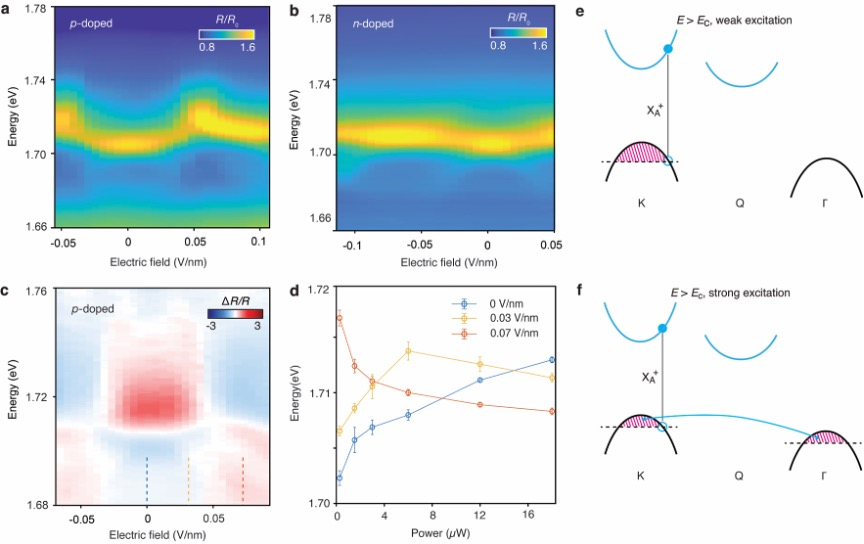
\includegraphics[width=1\textwidth]{Figures/C5/Fig5_13.jpg} % 
\end{center}
\caption[Electric-field dependent exciton energy and nonlinearity in homotrilayer WSe$_2$ at $T = 4$~K.] 
{\textbf{Electric-field dependent exciton energy and nonlinearity in homotrilayer WSe$_2$ at $T = 4$~K.} \textbf{a, b}, Electric-field dependence of the intralayer Fermi polaron reflectance contrast $R/R_{0}$ in trilayer with \textbf{(a)} hole and \textbf{(b)} electron doping density of $4.9 \times 10^{12}$~cm$^{-2}$. 
\textbf{c}, Reflectance change induced by a pulsed laser excitation of 12~$\mu$W power. 
The color map is obtained the same way as Figure~\ref{fig.5.6} d. 
Under a small electric field, X$_A^+$ shows a blueshift but it begins to redshift under excitation at higher electric fields. 
\textbf{d}, Line plots of the X$_A^+$ power-dependent peak shift under different electric fields. 
The X$_A^+$ shows a blueshift of $\sim$10~meV under zero applied electric field and a redshift of similar magnitude under large electric fields. 
The corresponding electric fields for these linecuts are indicated by the dashed lines in \textbf{(c)}. 
The error bars represent the uncertainty in determining the peak energy when fitting the reflection data. 
\textbf{e, f}, An electric field induces a shift of the valence band edge from $\Gamma$ to $K$ valley. 
Under strong optical pumping, a net valley polarization is induced by exciton--carrier scattering with increased carriers at the $\Gamma$ point, which leads to the optically induced redshift of X$_A^+$ at higher electric fields. 
In the nonequilibrium states, the dashed lines are used as indications for the carrier populations, and do not represent the Fermi level.}
\label{fig.5.13}
\end{figure}
\end{quote}
\renewcommand{\baselinestretch}{2}
\small\normalsize
% %/////////////////////// 

Intriguingly, the electric field also dramatically changes the nonlinear responses of X$_A^+$. 
As shown in Figure~\ref{fig.5.13}c, the reflectance change induced by optical pumping, $\Delta R/R$, shows a clear flip in the color contrast at $\sim$0.05~V/nm, which coincides with the crossover field between the blueshift and redshift of X$_A^+$ in Figure~\ref{fig.5.13}a. 
The magnitude of the blueshift and redshift is similar under the same excitation conditions, around 10~meV (Figure~\ref{fig.5.13}d). 
Such electric-field control of optical nonlinearity provides additional supporting evidence for our proposed mechanism involving valley polarization (Figures~\ref{fig.5.13} e,f). 
Figure~\ref{fig.5.13} e shows the modified band structure above the critical field~\cite{ref22}. 
Under optical excitation, the same exciton--hole scattering process can induce a population transfer of holes from $K$ to $\Gamma$, and reduce the X$_A^+$ energies (Figure~\ref{fig.5.13} f). 
This also explains the similar critical electric fields where both nonlinearity and electric-field susceptibility turn from blue- to redshift.

%////////////////////////////Figure Panel//////////////////
%Fig.5.14--------------
\vspace{2em}
\renewcommand{\baselinestretch}{2}
\small\normalsize
\begin{quote}
\begin{figure}[htbp]
\begin{center}
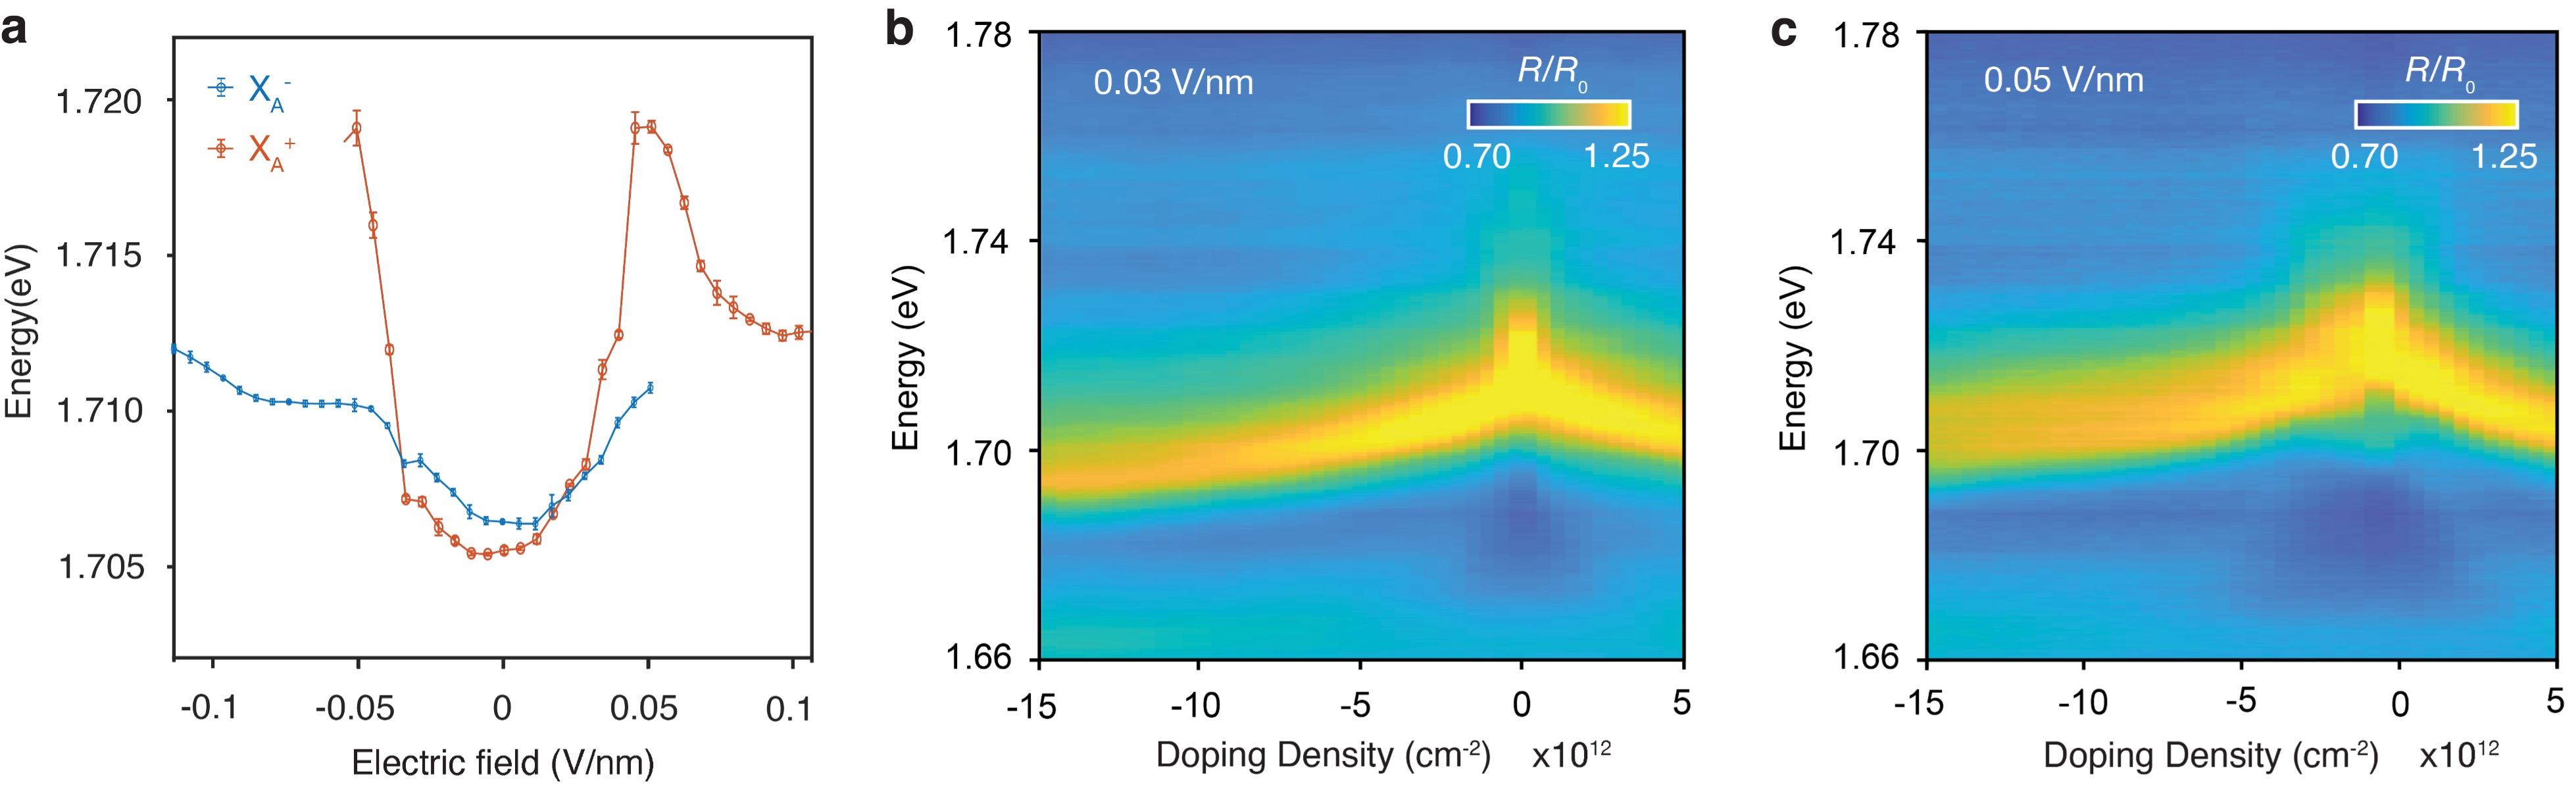
\includegraphics[width=1\textwidth]{Figures/C5/Fig5_14.jpg} % 
\end{center}
\caption[Electric-field tuning of Fermi polarons.] 
{\textbf{Electric-field tuning of Fermi polarons.} 
\textbf{a}, Energy shift of X$_A^-$ and X$_A^+$ with applied electric field at constant doping. 
The electron and hole doping densities are both kept at $4.9 \times 10^{12}$~cm$^{-2}$. 
The peak position is obtained by fitting the reflectance spectra with a Lorentzian model. 
The error bars represent the variance of the fitted peak energy.  
\textbf{b, c}, Doping dependence of the intralayer Fermi polaron reflectance contrast $R/R_{0}$ in trilayer with applied \textbf{(b)} 0.03~V/nm, \textbf{(c)} 0.05~V/nm electric field. 
The negative doping density represents the hole-doped side. 
An obvious blueshift and broadening of X$_A^+$ is observed on the hole side with increasing electric field, corresponding to additional phase-space filling due to the population transfer from $\Gamma$ to $K$ valleys. 
Such a shift is much weaker on the electron side.}
\label{fig.5.14}
\end{figure}
\end{quote}
\renewcommand{\baselinestretch}{2}
\small\normalsize
% %/////////////////////// 

\newpage
\section{Conclusions}
Our results demonstrating highly nonlinear excitons with large oscillator strengths open avenues for engineering exciton--carrier interactions in atomically thin heterostructures to explore strongly interacting many-body physics and develop novel optoelectronics. 
By designing the atomic and electronic structures of the heterostructures, one may engineer the strong interactions between bright, dark excitons, and free charges~\cite{ref26}. 
The excitonic and free charge populations are highly tunable, and elucidating the complex interactions between intralayer, interlayer excitons, and charges will be of significant future interest for studying many-body physics in a hybrid Fermi--Bose system~\cite{ref41,ref42,ref43}, from both theoretical and experimental perspectives. 
These strongly interacting optical excitations can be used to realize active nonlinear metasurfaces based on spatial confinement of excitons by moiré superlattices and local electrostatic gates~\cite{ref44,ref45,ref46}. 
Combining strong nonlinearity with spatial confinement could also further boost nonlinearity and allow exploring quantum optical effects, including nonclassical light sources and few-photon nonlinearity~\cite{ref11,ref47}. 
While current experiments require $10^3$--$10^4$ photons to shift the resonance by a linewidth, improving materials quality and engineering the photonic environment could lower the required photon count significantly by reducing the Fermi polaron linewidth. 
Finally, the demonstrated optical control of exciton resonances could enable novel nonlinear optoelectronic devices such as all-optical switching, nonlinear optomechanical resonators~\cite{ref48,ref49}, and optical limiting devices~\cite{ref4,ref50}.
%Chapter 6

\renewcommand{\thechapter}{6}

\chapter{Enhancing optical nonlinearity through \texorpdfstring{\\}{ }microcavity system }
\label{chap6}

\section{Introduction}
% An emerging field of quantum nonlinear optics seeks to achieve strong nonlinearity with lower power and ultimately even at the few-photon level. 
% This has been a significant goal in both classical and nonclassical optics, as it enables energy-efficient devices such as optical switches, single-photon transistors, and gates~\cite{ref1,ref2,ref3,ref4}. 
% However, photons, as the fundamental units of light, generally do not interact with each other unless under very specific conditions. 
% One approach to facilitate strong photon--photon interactions is by integrating materials with strong nonlinearities. 
% For example, systems such as single atoms~\cite{ref5,ref6}, molecules~\cite{ref7}, and atomic defects in solids~\cite{ref8}, where the reflectance and absorption of the particle can be modified by a single photon with inherently strong nonlinearities. 
% Such nonlinearity can be considered as, for instance, third-order nonlinearities such as saturable absorption with a saturation intensity corresponding to one photon per lifetime~\cite{ref9}. 
% However, a major challenge to demonstrate single-photon nonlinearity lies in the deterministic coupling of light to these emitters, such as embedding them in optical resonators~\cite{ref4,ref5,ref6,ref10}. 

% An alternative approach involves using extended optical excitations, such as excitons in semiconductors. 
% Excitons have larger oscillator strengths, which lead to stronger coupling to light, making them a promising candidate for achieving the desired nonlinear interactions~\cite{ref11}. 
% The exciton density-dependent resonance leads to third-order nonlinearity, which can be both dispersive and dissipative. 
% The challenge, however, lies in the relatively weak nonlinearities due to the weak interactions among excitons that are charge neutral. 
% For instance, in 2D semiconductors such as monolayer MoSe$_2$~\cite{ref12}, the excitonic nonlinearity induced by the exciton--exciton interaction can be observed as exciton blueshift under pulsed laser excitation. 
% The interaction strength, $g_{\mathrm{exc}}$, is defined as the energy shift induced per unit area density of excitons. 
% Rather generally, the exciton--exciton interaction $g_{\mathrm{exc}}$, dominated by exchange interactions, is on the order of $\sim E_B R_b^2$, where $E_B$ is the exciton binding energy and $R_b$ is the exciton Bohr radius. 
% Notably, a smaller Bohr radius leads to tighter binding of excitons, which makes $g_{\mathrm{exc}}$ more or less agnostic of materials, on the order of $\sim \mu$eV$\cdot\mu$m$^2$, whether in TMDs or GaAs quantum wells~\cite{ref13}.

% Given the intrinsically weak exciton--exciton interactions, various strategies are being pursued to enhance nonlinearity to the few-photon regime. 
% A prominent approach involves integrating optical materials with cavities or waveguides~\cite{ref19,ref20}. 
% For example, embedding TMDs into optical cavities leads to the formation of exciton--polaritons---a state that is half-light and half-matter---when the energy exchange between photons and excitons occurs faster than their respective decay rates. 
% This strong light--matter coupling is typically characterized by the emergence of two polariton states with distinct energies---lower and upper polaritons~\cite{ref21}. 
% The coupling strength, also known as vacuum Rabi splitting, can be determined by observing the anti-crossing behavior between excitons and photons. 
% Crucially, polaritons often exhibit different nonlinear responses compared to bare excitons. 
% In particular, the nonlinearity of polariton can be expressed as the susceptibility:  
% \begin{equation}
% \chi^{(3)}(r) = \frac{16 g_{\mathrm{exc-ph}}^{4}}{|\Gamma|^{2} \Gamma} \cdot \frac{i U(r)}{\Gamma + i U(r)} 
% \label{eq:susceptibility}
% \end{equation}
% where $g_{\mathrm{exc-ph}}$ is the coupling strength between exciton and photon, $U(r)$ is the interaction strength between two excitons at distance $r$, and $\Gamma$ is the linewidth. 
% Meanwhile, the cavity modifies the linewidth of the excitons, often reducing the number of photons required to shift the resonance by a linewidth.  

% Last but not least, with increasing pumping intensity, the vacuum Rabi splitting between the two polaritons also decreases, leading to the energy shift of polaritons~\cite{ref22,ref23}. 
% The reduction in the splitting is due to phase-space filling~\cite{ref24}, where more exciton population leads to fewer excitons left to couple to the cavity photon, similar to saturable absorption. 
% In fact, the Rabi splitting strength $\Omega$ depends on the polariton density:  
% \begin{equation}
% \Omega = 2g \left(1 - \frac{n \pi R_b^2}{2}\right)
% \label{eq:rabi}
% \end{equation}
% which leads to a phase-space-filling-induced nonlinearity, with the strength quantified as $g_{\mathrm{pol-pol}} \propto a_b^2 \hbar \Omega$~\cite{ref25}.
% At low density, the exchange interactions from the excitonic component dominate the polariton nonlinearity, resulting in a blue shift of both polariton branch resonances~\cite{ref26}.  

% TMDs offer several appealing features for exploring the nonlinear interaction of polaritons in the strong light--matter coupling regime. 
% With excitons in TMDs possessing large binding energies ranging from 200 to 500~meV and large oscillator strengths, strong coupling can persist even at room temperature with possibly enhanced exciton-mediated nonlinearity~\cite{ref27}. 
% The nonlinearity of polaritons generated in TMDs varies significantly depending on the specific species coupled to the cavity photon. 
% In monolayer WSe$_2$, the 2s exciton--polaritons exhibit a larger nonlinearity of approximately $46.4 \pm 13.9~\mu$eV$\cdot\mu$m$^2$, which is about four times larger than that of the 1s state~\cite{ref24}. 
% This difference is expected, given the larger Bohr radius of the 2s exciton. 
% Biexciton polaritons also exhibit a nonlinear interaction boost~\cite{ref28}. 
% Phase-space filling was thought to play an important role in the measured nonlinear response in TMD polaritons. 
% Similarly, trion--polaritons in monolayer MoSe$_2$ microcavities exhibit enhancement of the nonlinearity strength of $\sim 37 \pm 3~\mu$eV$\cdot\mu$m$^2$ at a low electron density and pump fluence~\cite{ref29}, driven by the strong band-filling effect. 
% However, the increased nonlinearity observed in 2s exciton- and trion-polaritons comes at the cost of reduced coupling strength between the optical excitation and the photons due to their weaker oscillator strength.  

% Another approach uses interlayer excitons with stronger dipolar repulsion, such as those in bilayer MoS$_2$~\cite{ref15}. 
% Such interlayer excitons can have sufficient oscillator strength to enable strong coupling when the carrier tunneling in the material is large enough to produce hybridization between interlayer and intralayer states~\cite{ref30}. 
% Combining this IX exciton with cavity photons forms the dipolar interlayer polariton, which has a ten-fold enhancement of the nonlinearity strength ($g_{\mathrm{IX}} \sim 100 \pm 2~\mu$eV$\cdot\mu$m$^2$) compared with the conventional intralayer exciton ($g_A \sim 10 \pm 0.2~\mu$eV$\cdot\mu$m$^2$) embedded in a microcavity~\cite{ref15,ref31}.  

% An intriguing set of recent experiments uses the moiré superlattice in 2D materials to demonstrate strong nonlinearity in exciton--polariton systems~\cite{ref32}. 
% With the moiré excitons confined within each site, they experience strong on-site interactions~\cite{ref33,ref34,ref35}, which suggests that exciton blockade can occur when the average exciton--exciton density is close to the size of the moiré cell, on the order of a few to tens of nanometers, much larger than the blockade radius of bare excitons. 
% Meanwhile, the exciton and photon can still couple collectively among all the cells, which maintains the system in a strong coupling regime.  

% With the above developments, it has become more feasible for this system to finally enter the quantum nonlinear optics regime when the polariton nonlinear interaction strength surpasses the linewidth. 
% In such a case, the optical response of the system is significantly altered by the presence of a single photon, leading to unprecedented phenomena and technologies in solids. 
% One example is the so-called photon blockade~\cite{ref36,ref37}, where a single polariton can inhibit the transmission of additional photons. 
% Such photon blockade effects can be observed through photon antibunching and could open exciting avenues for realizing nonclassical light sources in quantum nonlinear optics~\cite{ref38,ref39,ref40,ref41}.  

Strong optical nonlinearities at the few-photon level are highly sought after for energy-efficient photonic and quantum devices, such as all-optical switches, transistors, and gates~\cite{Hwang2009-rg,Turchette1995-nv,Chang2007-lw,Volz2012-pb}. 
Yet photons do not naturally interact, and achieving such effects requires materials or systems with enhanced nonlinear responses.  

Early approaches used individual quantum emitters such as atoms, molecules, or defects, where a single photon can substantially alter absorption or reflectance~\cite{Birnbaum2005-ix,Schuster2008-nv,Lounis2000-iy,Castelletto2014-pv}. 
While these systems demonstrate strong nonlinearities, their practical use is limited by the challenge of deterministically coupling photons to isolated emitters~\cite{Harris1990-ej,Fushman2008-lk}.  

Excitons in semiconductors offer a collective platform, with large oscillator strengths that enable strong light--matter coupling\cite{Wang2018-my}.
However, because excitons are charge neutral, their mutual interactions are relatively weak, producing nonlinearities on the order of only a few $\mu$eV$\cdot\mu$m$^2$ across both TMDs and quantum wells~\cite{Scuri2018-bn,Shahnazaryan2017-gx}.  

Embedding excitons in optical cavities forms exciton--polaritons, hybrid light--matter quasiparticles that inherit both strong coupling and nonlinear response~\cite{Liu2015-hm,Deng2010-ul}. 
Compared with bare excitons, polaritons show enhanced nonlinearities due to modified linewidths and collective light--matter interactions. 
The polariton nonlinear shift can be contributed from the exciton-exciton interaction at lower exciton population desntiy\cite{Gu2021-cu,Ciuti2003-zj} and phase-space filling,
where exciton saturation reduces the available oscillator strength~\cite{Song2024-na,Gu2021-cu}.  

TMD monolayers provide an especially attractive platform due to their large binding energies (200--500 meV) and strong oscillator strengths, enabling robust polariton formation even at room temperature~\cite{Wang2018-my}. 
Recent studies have reported enhanced nonlinearities in higher-order exciton states, biexcitons, and trions~\cite{Gu2021-cu,Wei2023-by,Emmanuele2020-oh}, though these gains can come at the cost of weaker light coupling. 
Interlayer excitons, with their strong dipole--dipole repulsion, and moiré-confined excitons further offer routes to boost polariton interactions by an order of magnitude or more~\cite{Datta2022-po,Leisgang2020-mn,Louca2023-in,Zhang2021-eb}.  

These advances suggest that exciton--polaritons in 2D materials are a promising pathway toward the quantum nonlinear optics regime, where the interaction strength exceeds the linewidth. 
In this limit, a single polariton can block the transmission of others, giving rise to photon blockade and enabling nonclassical light sources~\cite{A-Verger-C-Ciuti-and-I-Carusotto2006-wd,Munoz-Matutano2019-cg,Somaschi2016-uk,He2013-od,Turunen2022-wom,Delteil2019-pp}.  

In this work, we present a method to utilize a 1D microcavity with highly confined photons to couple with the Fermi polaron in homotrilayer WSe$_2$, aiming to further enhance the nonlinearity and reduce the number of photons required for photon blockade. 
We first designed this high-quality microcavity with highly reflective dielectric Bragg mirrors (TiO$_2$ and SiO$_2$) for the designed wavelength of light (730~nm). 
We then embed the trilayer WSe$_2$ device with monolayer/bilayer graphene as dual gates into this microcavity. 
Thanks to the large oscillator strength of the excitons and polarons in the trilayer WSe$_2$, we can enter a strong coupling regime between the exciton/polaron and the photon---indicated by the signature of the formation of polaritons, which can be tuned by electrical gating.

\section{Design of gate compatible 1D microcavity}
\subsection{Cavity simulation}
Embedding TMDs or other 2D materials with a 1D microcavity has already been demonstrated~\cite{cite}. 
However, the overall quality factor of the cavity can be low due to the large inhomogeneous nature of the van der Waals structure. 
As a result, gate-dependent control of polaritons is seldom studied, as the gating material graphite has high optical loss, and adding it to the structure would further reduce the $Q$ value. 

Here, we tune the position of the graphite gate. 
By placing the graphite at the mode field minimum, the cavity loss can be greatly reduced. 
As shown in the schematic below, the total cavity length $l$ is given by the total thickness of the van der Waals stack. 
The cavity length is expressed as $l = \frac{m \lambda_{0}}{2 n_{\mathrm{hBN}}}$,
where $m$ is the mode number inside the cavity. 
For a mode value of $m=5$, we need four layers of hBN: two of them with thicknesses $l_{\mathrm{gr1}}$ and $l_{\mathrm{gr2}}$, and the other two with thicknesses of $\frac{1}{2} l_c$. 
Placing graphite at the node of the field gives the distance 
$l_{\mathrm{gr1}},\, l_{\mathrm{gr2}} = \frac{n \, l}{m}$ and the condition  
$l_{\mathrm{gr1}} + l_{\mathrm{gr2}} + l_c = l$.

%Fig.6.1--------------
% \vspace{1em}
\renewcommand{\baselinestretch}{1}
\small\normalsize
\begin{quote}
\begin{figure}[htbp]
\begin{center}
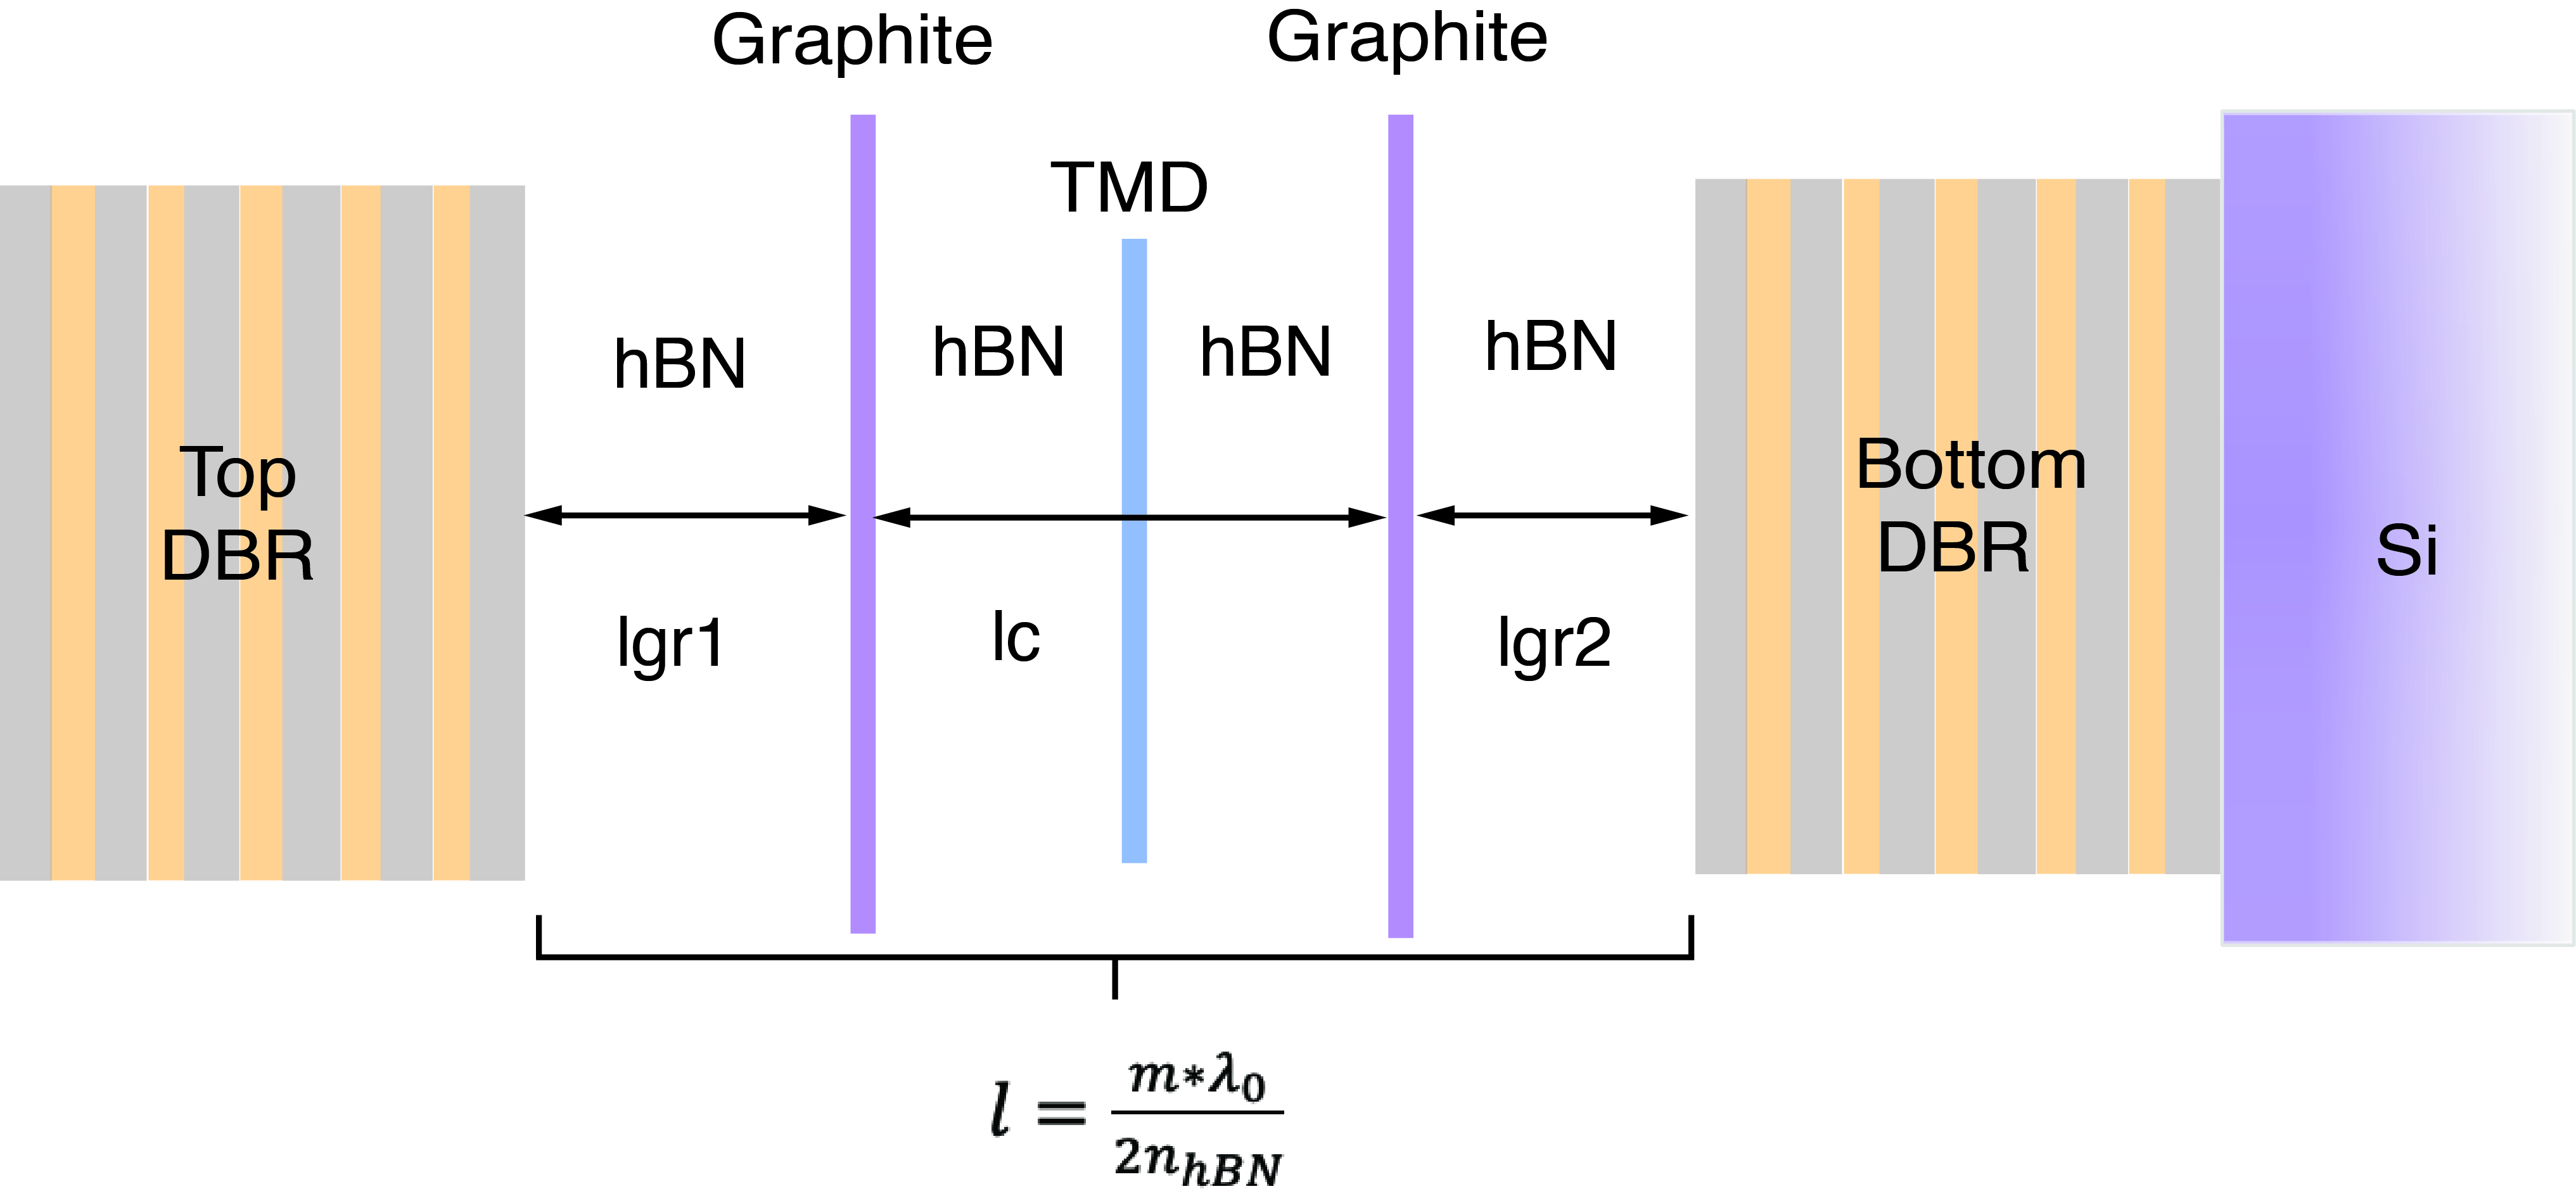
\includegraphics[width=0.7\textwidth]{Figures/C6/Fig6.1.jpg} % 
\end{center}
\caption[Schematic of van der Waals 1D microcavity design.] 
{\textbf{Schematic of van der Waals 1D microcavity design.}}
\label{fig.6.1}
\end{figure}
\end{quote}
\renewcommand{\baselinestretch}{2}
\small\normalsize
% %/////////////////////// 
Then by using the Transfer Matrix Method (TMM) with the optical indices of all constituent materials (hBN, graphite) and the thickness of each layer, we can simulate the field distribution and optimize the $Q$-factor of our proposed microcavity structure. 
Figure~\ref{fig.6.1} shows the schematic and the simulated reflectance spectrum of the microcavity with the embedded van der Waals stack (without TMD). 
According to our simulation, the cavity achieves a $Q$-factor of approximately 2500 at normal incidence (Figure~\ref{fig.6.2}).

%Fig.6.2--------------
% \vspace{1em}
\renewcommand{\baselinestretch}{1}
\small\normalsize
\begin{quote}
\begin{figure}[htbp]
\begin{center}
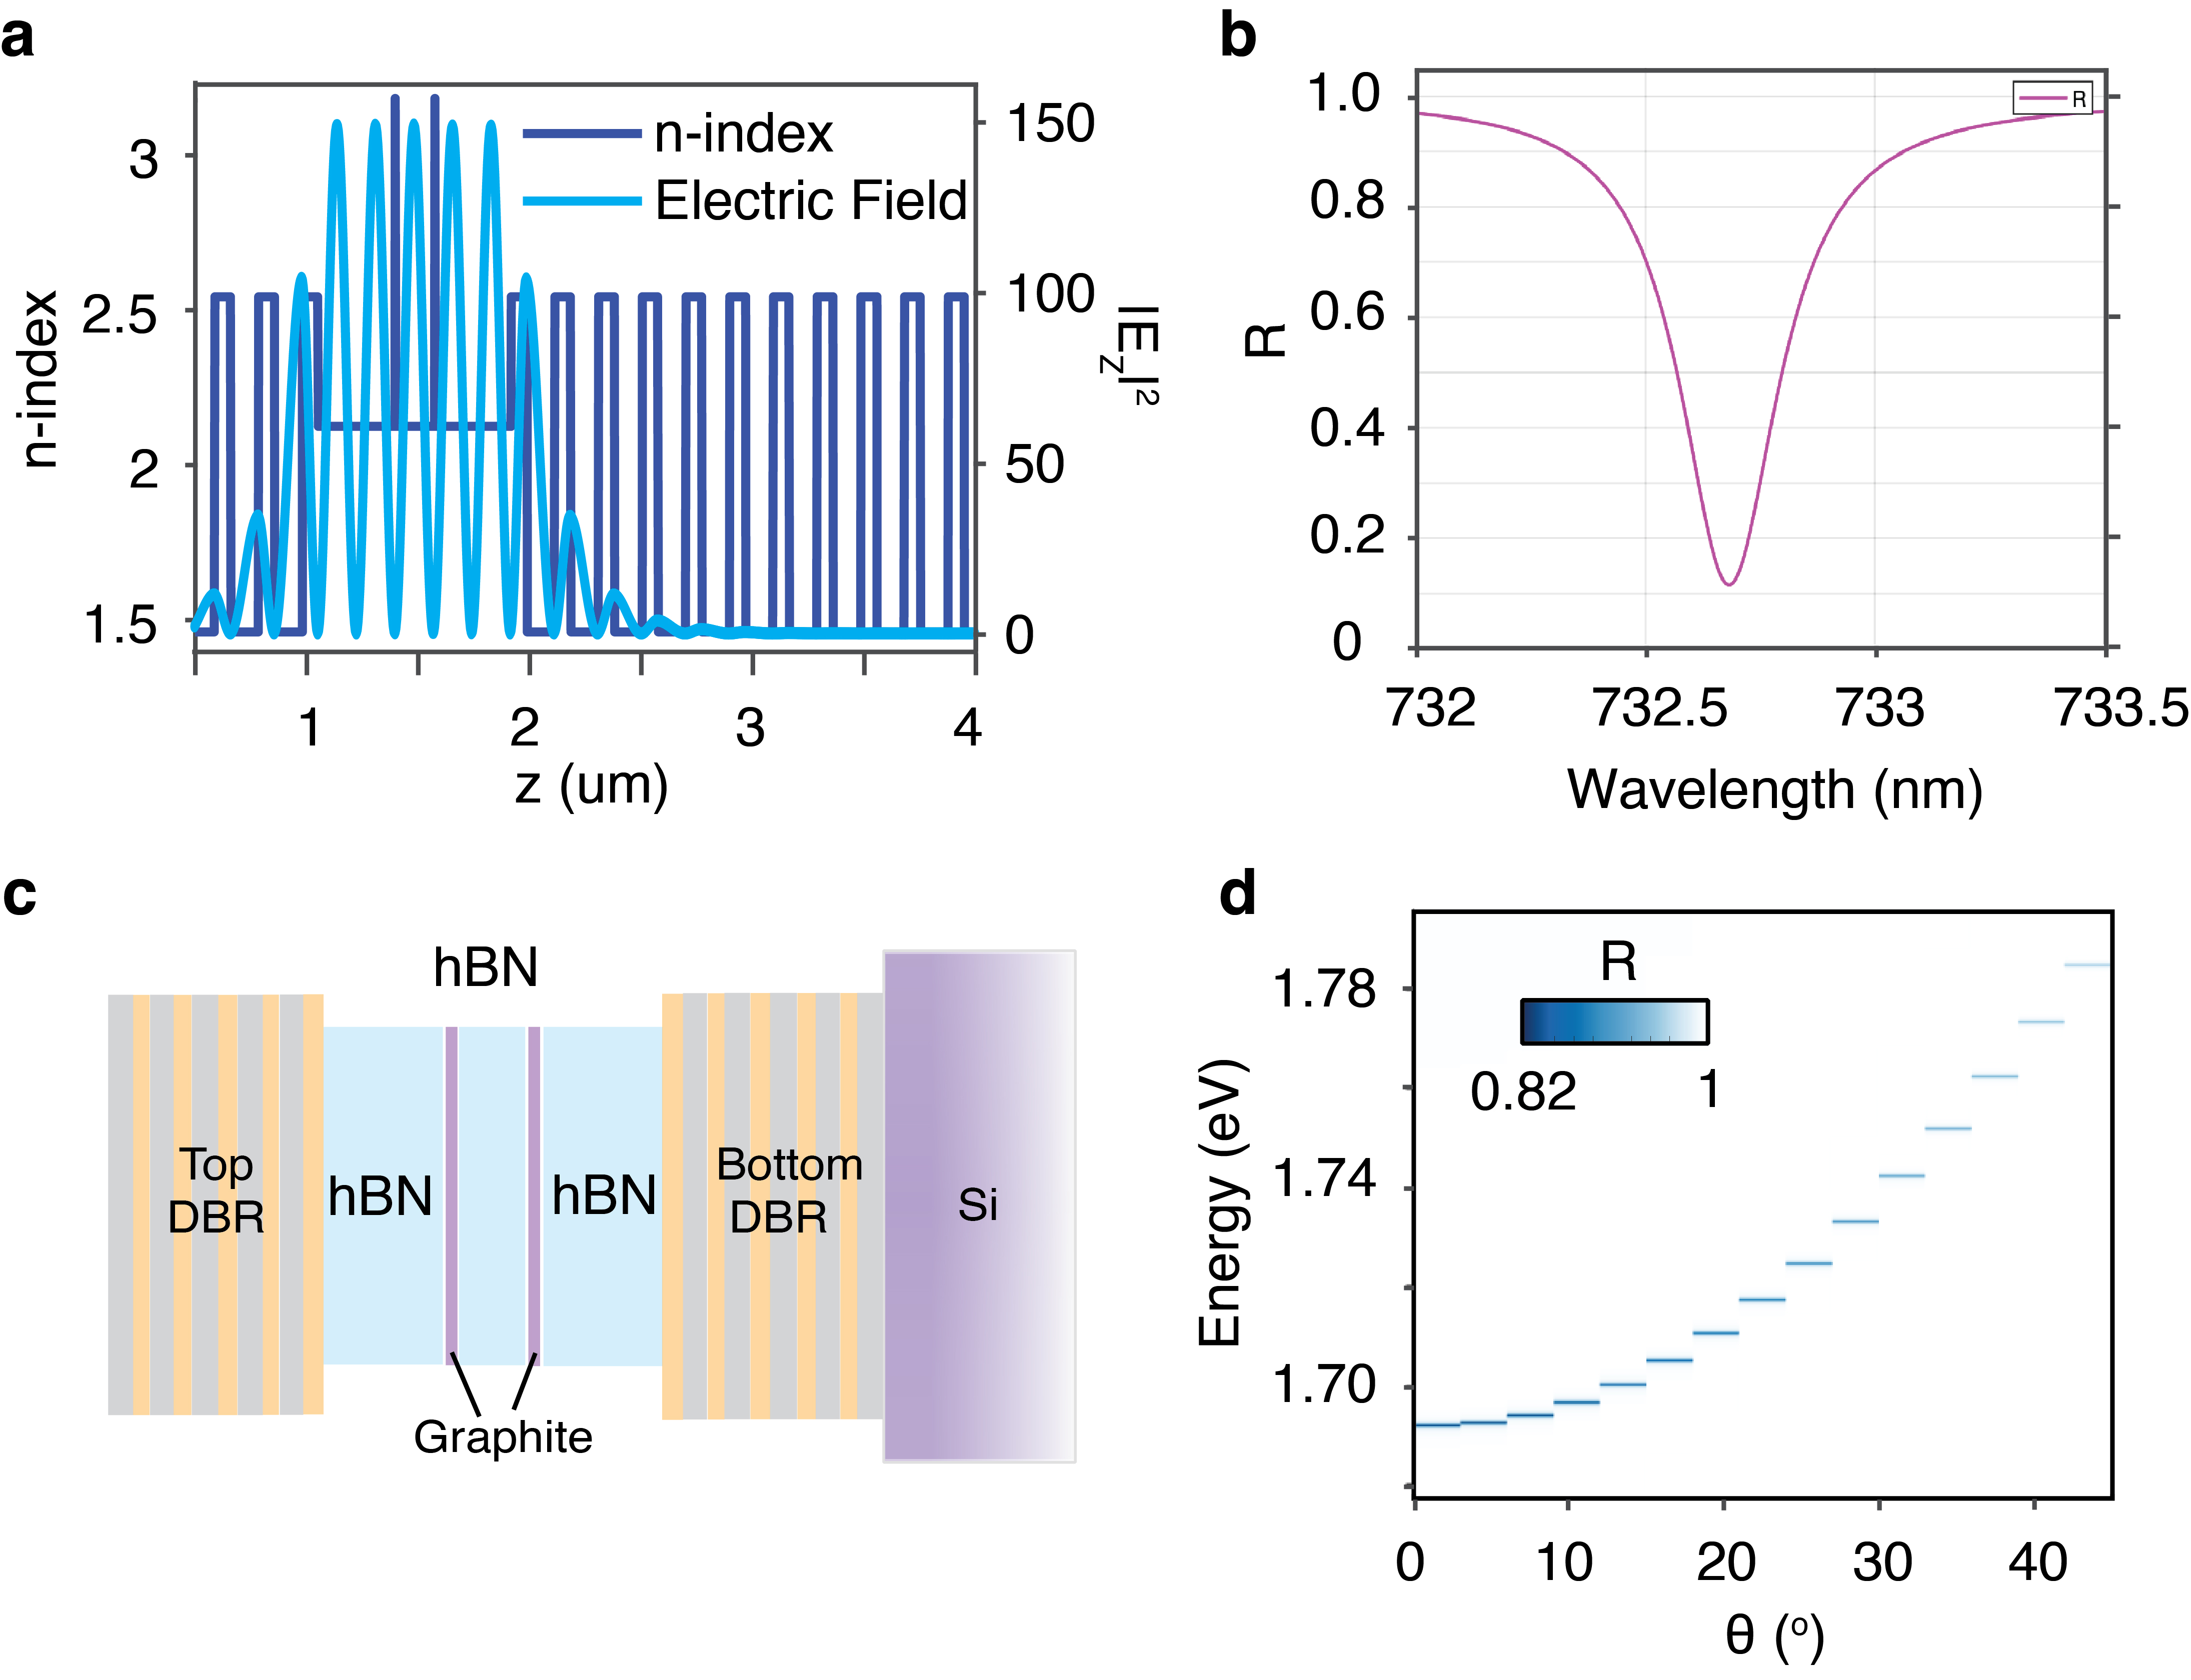
\includegraphics[width=0.8\textwidth]{Figures/C6/Fig6.2.jpg} % 
\end{center}
\caption[TMM simulation of high quality all-dielectric DBR encapsulated van der Waals microcavity simulation.] 
{\textbf{TMM simulation of high quality all-dielectric DBR encapsulated van der Waals microcavity simulation.}.\textbf{a,} The cavity structure and the field distribution along the $z$ direction (5 modes in cavity). \textbf{b,} Reflectance of the empty van der Waals microcavity. \textbf{c,} van der Waals stack embedded within the microcavity. \textbf{d,} cavity resonance energy tuning by the incident angle $\theta$.}
\label{fig.6.2}
\end{figure}
\end{quote}
\renewcommand{\baselinestretch}{2}
\small\normalsize
% %/////////////////////// 
\subsection{Polariton simulation}
We then integrate the trilayer WSe$_2$ into this high-$Q$ cavity and simulate the polariton dispersion. 
At first, we extract the dielectric function of the trilayer WSe$_2$ A exciton transition based on the Lorentzian model\cite{}:  
\begin{equation}
\varepsilon(\omega) = \varepsilon_{\infty} + \frac{f \omega_{0}^{2}}{\omega_{0}^{2} - \omega^{2} - i \Gamma \omega}
\label{eq:Lorentz}
\end{equation}
where $\varepsilon_{\infty}$ is the dielectric response at high frequency (background permittivity), 
$f$ is the oscillator strength of the X$_A^+$ transition of the trilayer WSe$_2$, 
and $\Gamma$ is the linewidth of the exciton transition.  

We can thus calculate the dielectric function and extract $n$ and $k$ based on this model and fit it with our reflectivity spectrum of WSe$_2$ at 4~K (see Figure~\ref{fig.6.3}). 
The parameters used for the simulation are listed below:  
Resonant wavelength: 729.4~nm; oscillator strength $f$: 1.4; polaron linewidth: 10~meV; background permittivity: 25.9\cite{}.

%Fig.6.3--------------
% \vspace{1em}
\renewcommand{\baselinestretch}{1}
\small\normalsize
\begin{quote}
\begin{figure}[htbp]
\begin{center}
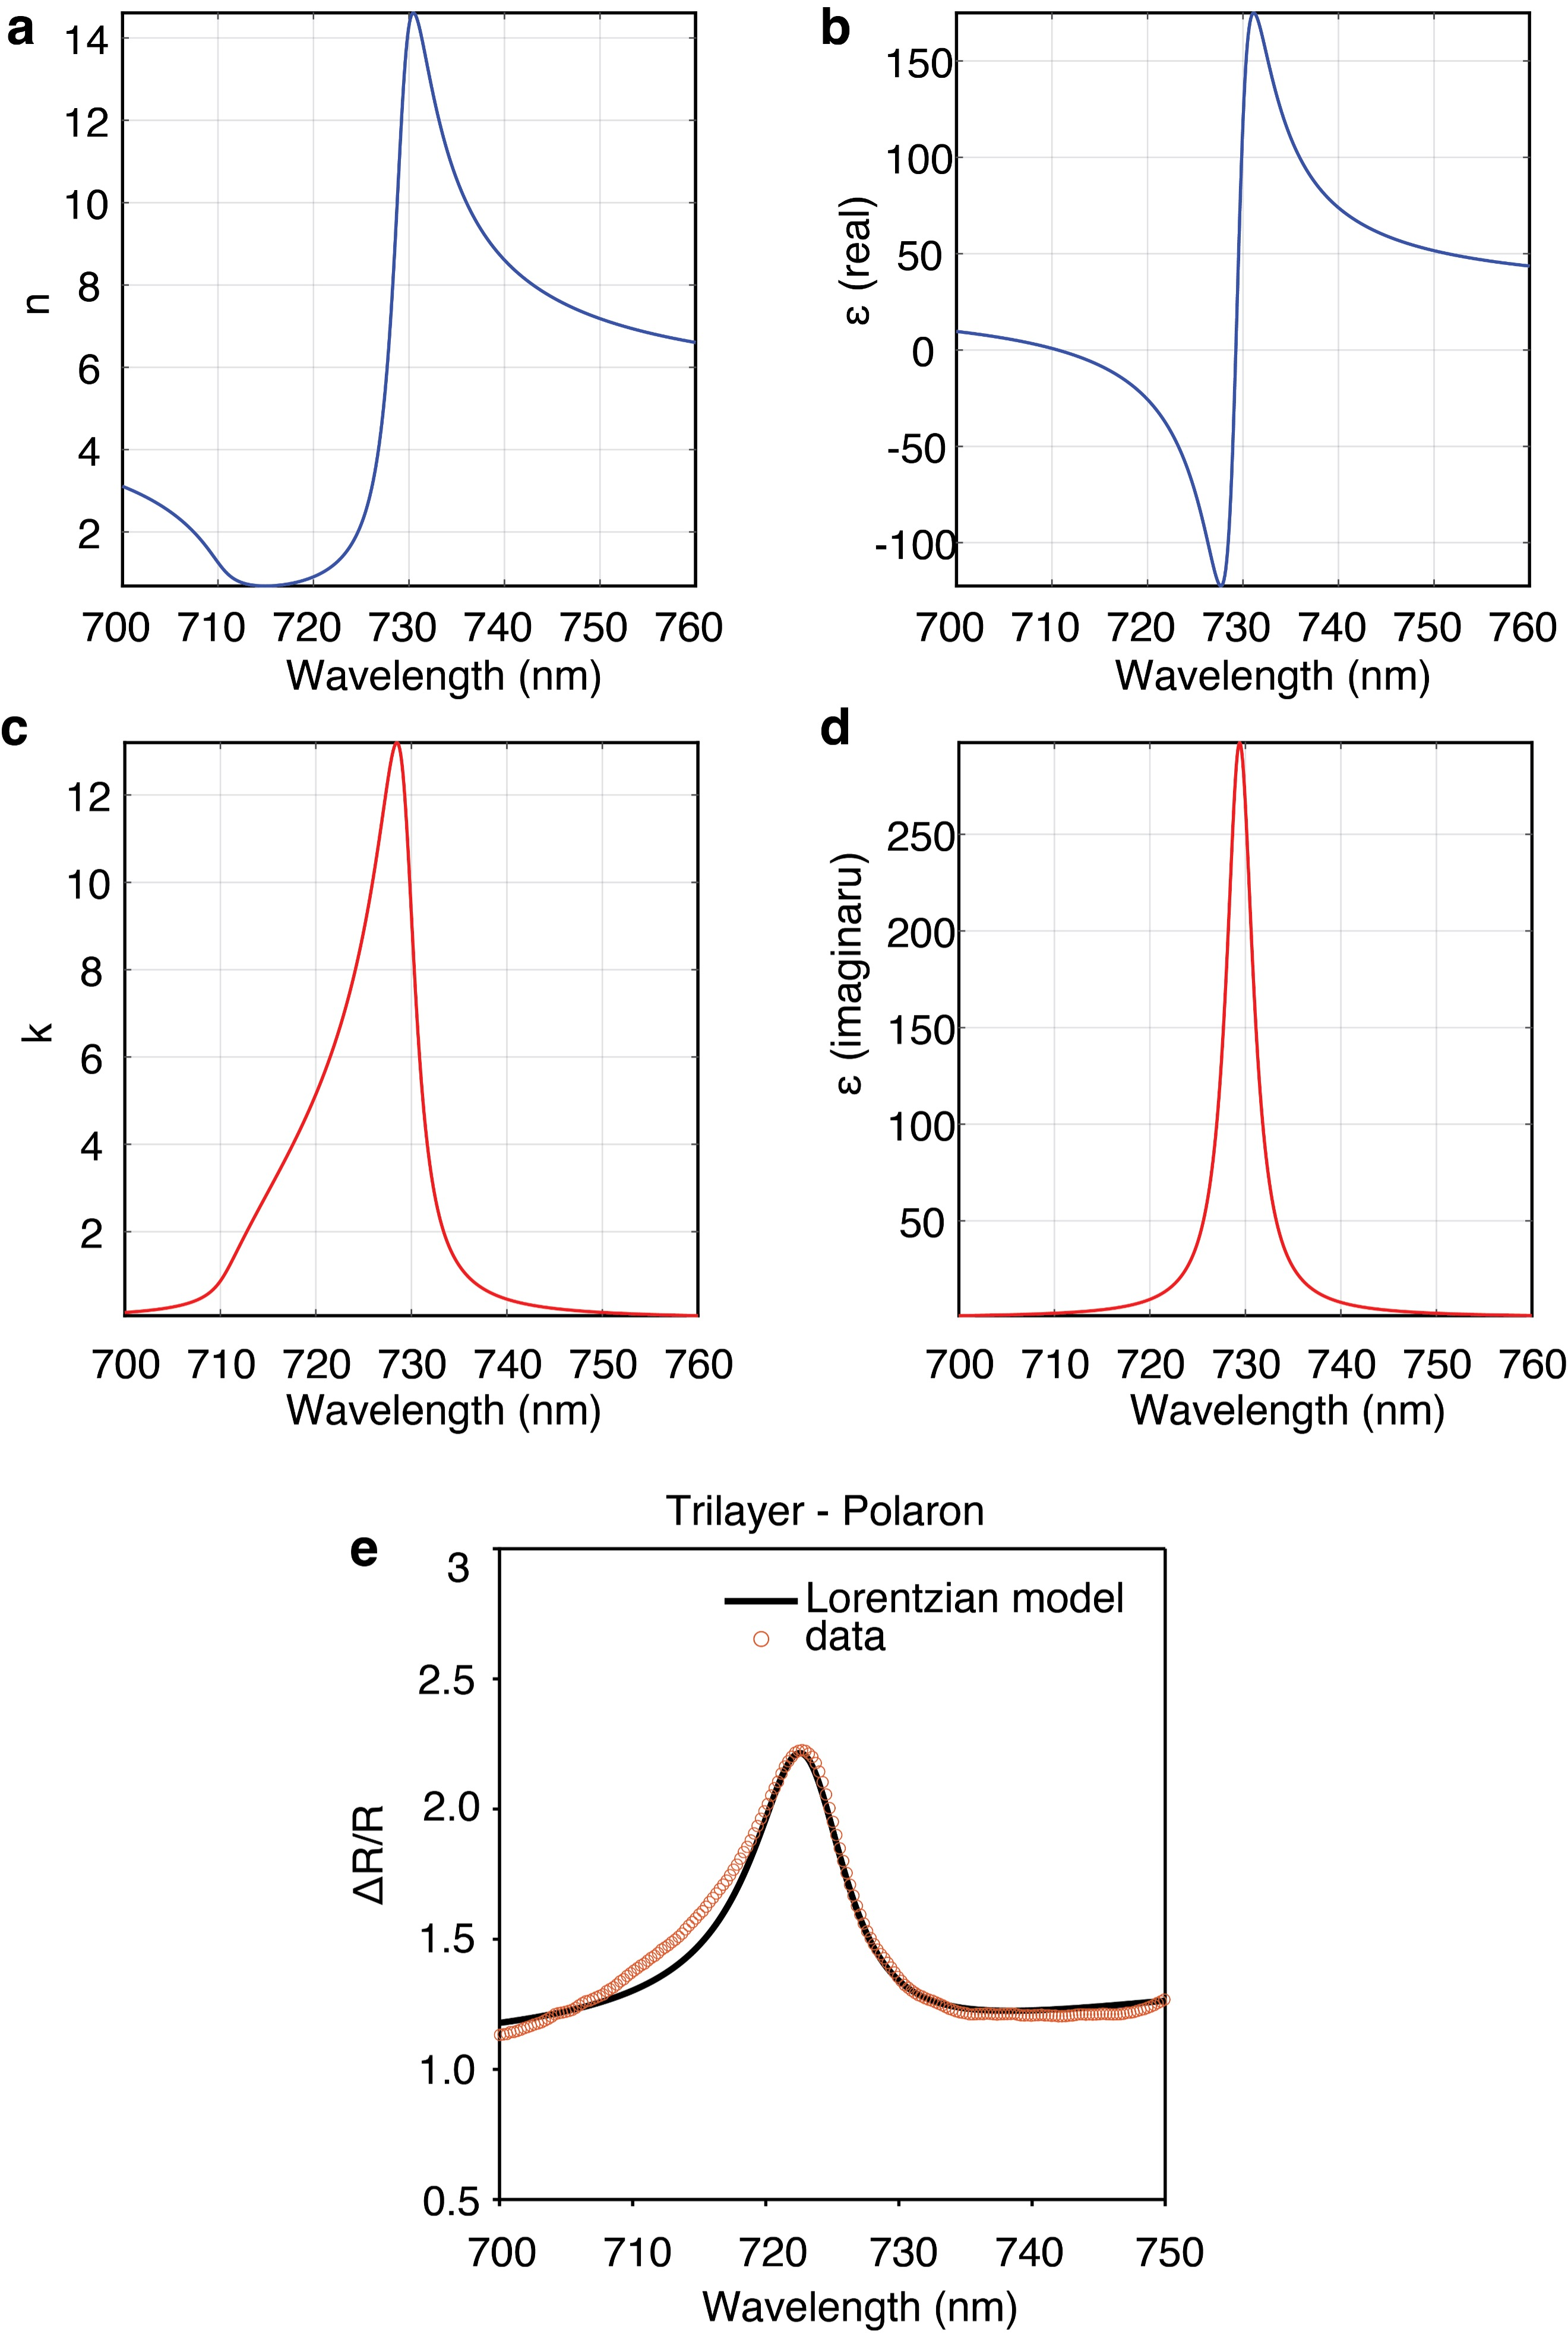
\includegraphics[width=0.65\textwidth]{Figures/C6/Fig6.3.jpg} % 
\end{center}
\caption[Calculated dielectric function and optical index of trilayer WSe$_2$ at $4$ K based on Lorentzian model.] 
{\textbf{Calculated dielectric function and optical index of trilayer WSe$_2$ at $4$ K based on Lorentzian model.}
\textbf{a,b,} Real part of the refractive index and dielectric function. \textbf{c,d,} Imaginary part of the refractive index and dielectric function. \textbf{e,} Comparison of the calculated trilayer WSe$_2$ reflectance and the experimental result.}
\label{fig.6.3}
\end{figure}
\end{quote}
\renewcommand{\baselinestretch}{2}
\small\normalsize
% %/////////////////////// 
When we insert the trilayer WSe$_2$ at the antinodes of the resonant field in the cavity, the exciton resonant with the cavity mode will strongly interact with optical field, leading to a new excitation quasiparticle called polariton. 
The energy of the lower and upper polariton can be derived as Eq.~\ref{eq:LP_UP} as we discussed in \ref{chap4} in the simulation.
Since polaritons are a superposition of the photon and exciton at the same $k_{\parallel}$, 
their fractions of exciton and photon components can be quantified by the squared amplitudes of the Hopfield coefficients $X_{k_{\parallel}}$ and $C_{k_{\parallel}}$. 
In the simulation, the coefficients are calculated based on the Eq.~\ref{eq:Hopcoefficient_Xk} and \ref{eq:Hopcoefficient_Ck}.

Since our objective is to realize nonlinear behavior in the lower polariton, we begin by employing a cavity mode that is resonant with the Fermi polaron(detuning $\Delta$ at zero). 
This configuration maximizes the exciton fraction in the lower polariton branch, thereby providing the most favorable conditions for observing nonlinear effects.

Figure~\ref{fig.6.4} shows the simulated polariton dispersion at $\Delta = 0$, from which we can extract the coupling strength of $\hbar \Omega \sim 42$~meV. While this condition highlights the anti-crossing that defines strong coupling, optimal device performance requires finite detuning. 

%Fig.6.4--------------
% \vspace{1em}
\renewcommand{\baselinestretch}{1}
\small\normalsize
\begin{quote}
\begin{figure}[htbp]
\begin{center}
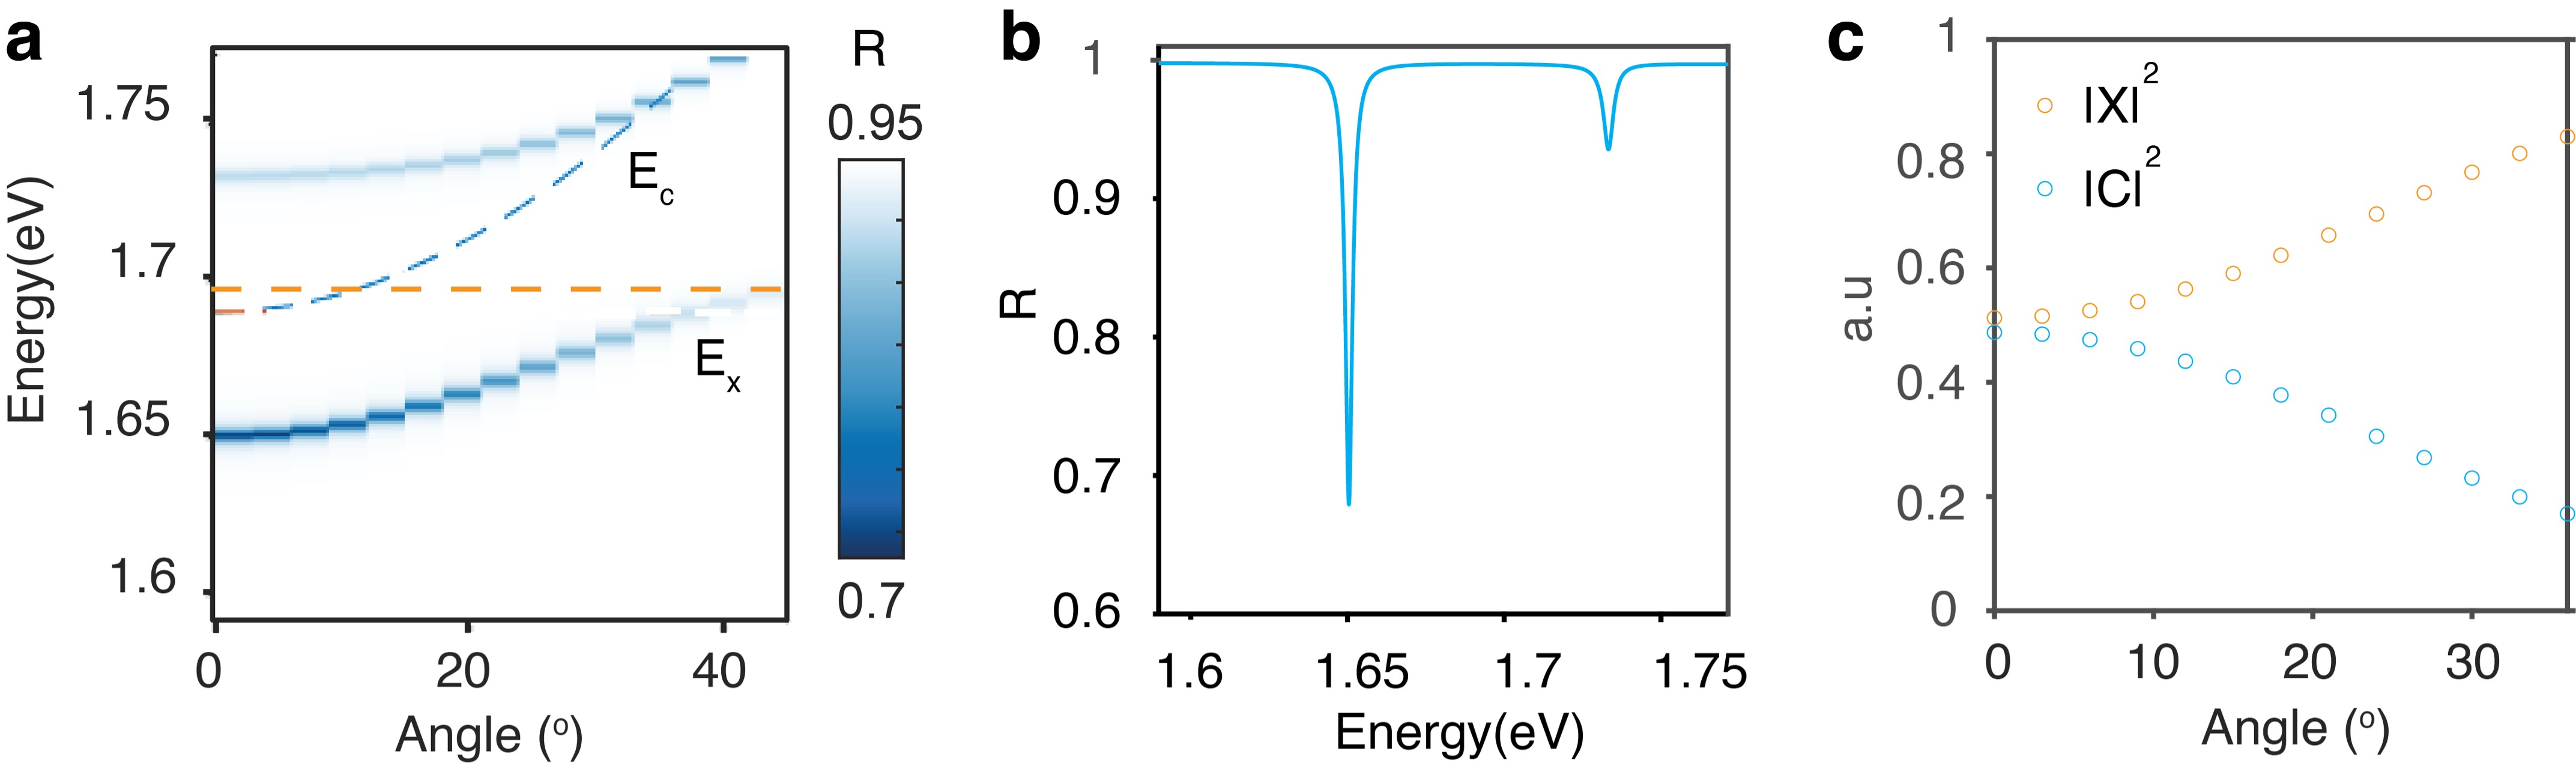
\includegraphics[width=1\textwidth]{Figures/C6/Fig6.4.jpg} % 
\end{center}
\caption[TMM simulation of trilayer WSe$_2$ embedded microcavity reflectance.] 
{\textbf{TMM simulation of trilayer WSe$_2$ embedded microcavity reflectance.}
\textbf{a,}Polariton dispersion at zero detuning ($\Delta = 0$) as a function of incident angle. 
The blue and orange dashed line refers to the cavity and exciton resonance, respectively. 
\textbf{b,} Reflectance spectrum of the polariton at normal incidence. 
\textbf{c,} Calculated Hopfield coefficient of the lower polariton branch.}
\label{fig.6.4}
\end{figure}
\end{quote}
\renewcommand{\baselinestretch}{2}
\small\normalsize
% %/////////////////////// 
Detuning $\Delta$ modifies the relative photon and exciton fractions of the polariton states. 
The polariton’s lifetime primarily inherits from the photon fraction $\lvert C_{k_{\parallel}} \rvert^2$, while nonlinear interactions inherit from the exciton fraction $\lvert X_{k_{\parallel}} \rvert^2$. 
Thus, achieving strong polariton–polariton interactions requires balancing excitonic interaction strength with photonic lifetime. 
This trade-off is quantified by:
$g \sim \lvert X_{k_{\parallel}} \rvert^4 \, U_{\mathrm{ex}}$
where $U_{\mathrm{ex}}$ refers to the exciton–exciton interaction strength. 

We examine a range of detuned conditions by modifying the cavity resonance through both the cavity length (hBN thickness) and the in-plane wavevector $k_{\parallel}$ (as shown in Figure~\ref{fig.6.5}).
According to the simulation results, larger excitonic fractions are obtained only for detuning values $\Delta\geq 0$. The maximum degree of antibunching is expected when the exciton and cavity photon are close to resonance. 
In this case, the required cavity hBN thickness is estimated to be 165–170 nm, corresponding to a cavity resonance near 730 nm. 

%Fig.6.5--------------
% \vspace{1em}
\renewcommand{\baselinestretch}{1}
\small\normalsize
\begin{quote}
\begin{figure}[htbp]
\begin{center}
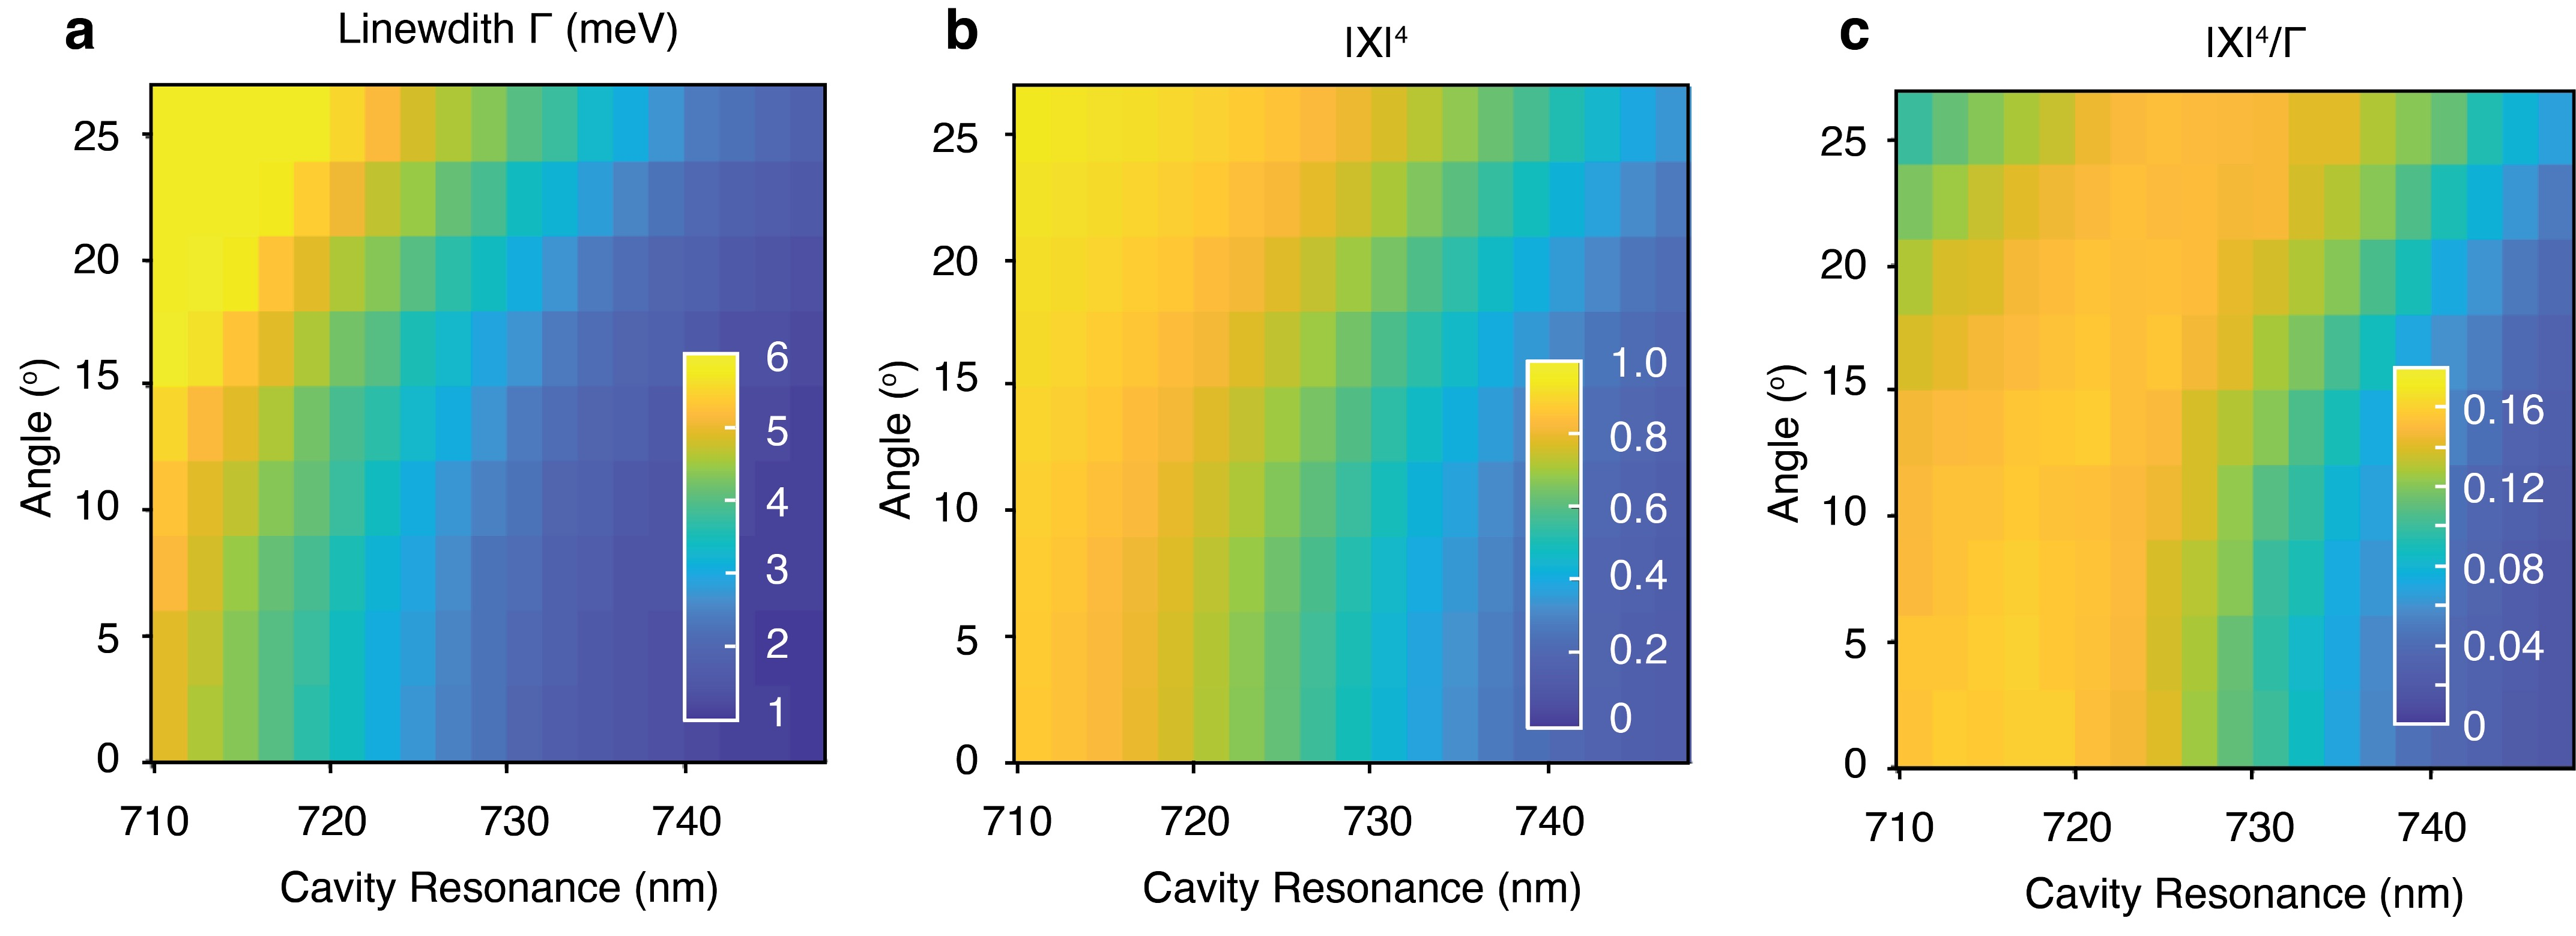
\includegraphics[width=1\textwidth]{Figures/C6/Fig6.5.jpg} % 
\end{center}
\caption[\textit{In situ} tuning lower polariton’s property via detuning $\Delta$.] 
{\textbf{\textit{In situ} tuning lower polariton’s property via detuning $\Delta$.}
\textbf{a}, Linewidth of the lower polariton as a function of cavity resonance and angle. 
\textbf{b}, Excitonic contribution $\lvert X_{k_{\parallel}} \rvert^4$ extracted from the Hopfield coefficient. 
\textbf{c}, Effective interaction strength parameter $\lvert X_{k_{\parallel}} \rvert^4 / \Gamma$ indicating the maximum degree of antibunching.
}
\label{fig.6.5}
\end{figure}
\end{quote}
\renewcommand{\baselinestretch}{2}
\small\normalsize
% %/////////////////////// 

\section{Sample Fabrication}
We used a bottom DBR stack comprising 12.5 pairs of TiO$_2$/SiO$_2$ films with alternating thicknesses of 340~nm/120~nm sputtered on 285~nm SiO$_2$/Si. 
This combination produces a stopband between 710--780~nm. 
Graphite and hBN flakes were then mechanically exfoliated from bulk crystals onto the silicon chip with a SiO$_2$ layer. 
The thickness of each layer was identified using Atomic Force Microscopy (AFM). 
Based on our Transfer Matrix Method (TMM) simulation, we selected 80~nm hBN (Device~1) / 90~nm hBN (Device~2) as the top and bottom encapsulation, which yields a cavity resonance close to the Fermi polaron. 
Monolayer graphene / bilayer graphite was chosen for the top and bottom gates due to the strong absorption of thick graphite in the visible range. 

The van der Waals heterostructures were assembled using a dry-transfer method with PDMS (polydimethylsiloxane) and PC (polycarbonate) as the stamp, sequentially stacking all the flakes onto the bottom DBR substrate. 
Electrical contacts were then defined by electron-beam lithography, followed by a liftoff process after thermal evaporation of 5~nm Cr and 100~nm Au. 
Finally, the silver top mirror (35--40~nm thick) was patterned using the same lithography and liftoff procedure. 
During the electron-beam lithography step for the silver mirror, a low beam current of 300~pA was employed to minimize potential degradation of the optical properties of the trilayer WSe$_2$ in the active region.
Figures~\ref{fig.6.6} shows the optical image of the fabricated devices.
Figures~\ref{fig.6.7} shows the device schematic and the simulated reflectace spectrum for D1 and D2.

%Fig.6.6--------------
% \vspace{1em}
\renewcommand{\baselinestretch}{1}
\small\normalsize
\begin{quote}
\begin{figure}[htbp]
\begin{center}
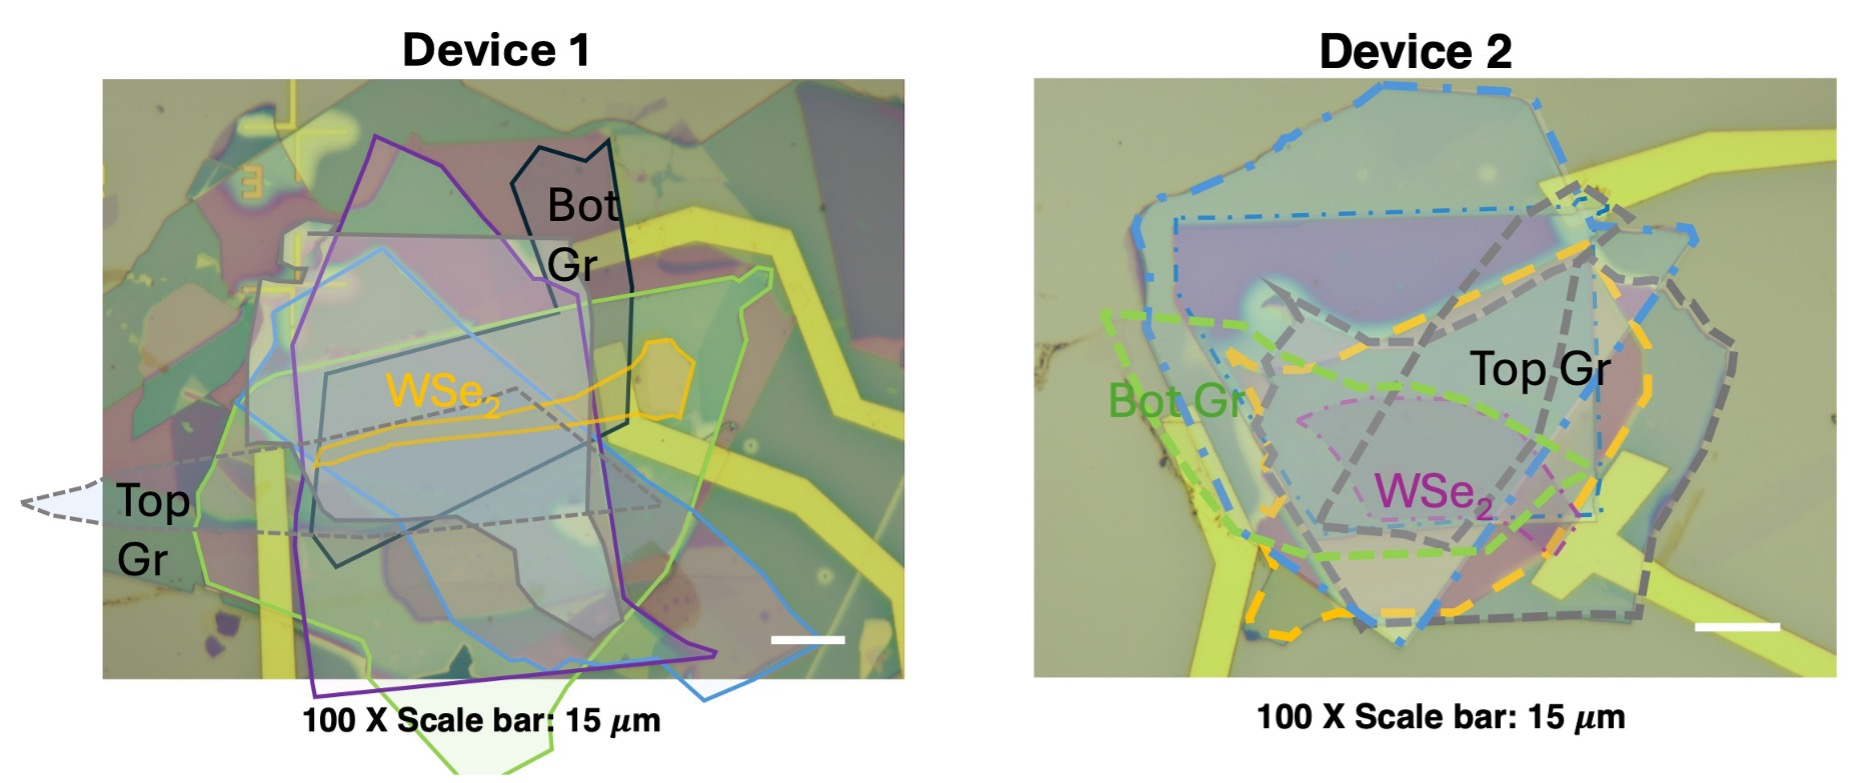
\includegraphics[width=1\textwidth]{Figures/C6/Fig6.6.jpg} % 
\end{center}
\caption[Optical image of the van der Waals microcavity Device 1 and 2 (without Ag)] 
{\textbf{Optical image of the van der Waals microcavity Device 1 and 2 (without Ag)}
}
\label{fig.6.6}
\end{figure}
\end{quote}
\renewcommand{\baselinestretch}{2}
\small\normalsize
% %/////////////////////// 
%Fig.6.7--------------
% \vspace{1em}
\renewcommand{\baselinestretch}{1}
\small\normalsize
\begin{quote}
\begin{figure}[htbp]
\begin{center}
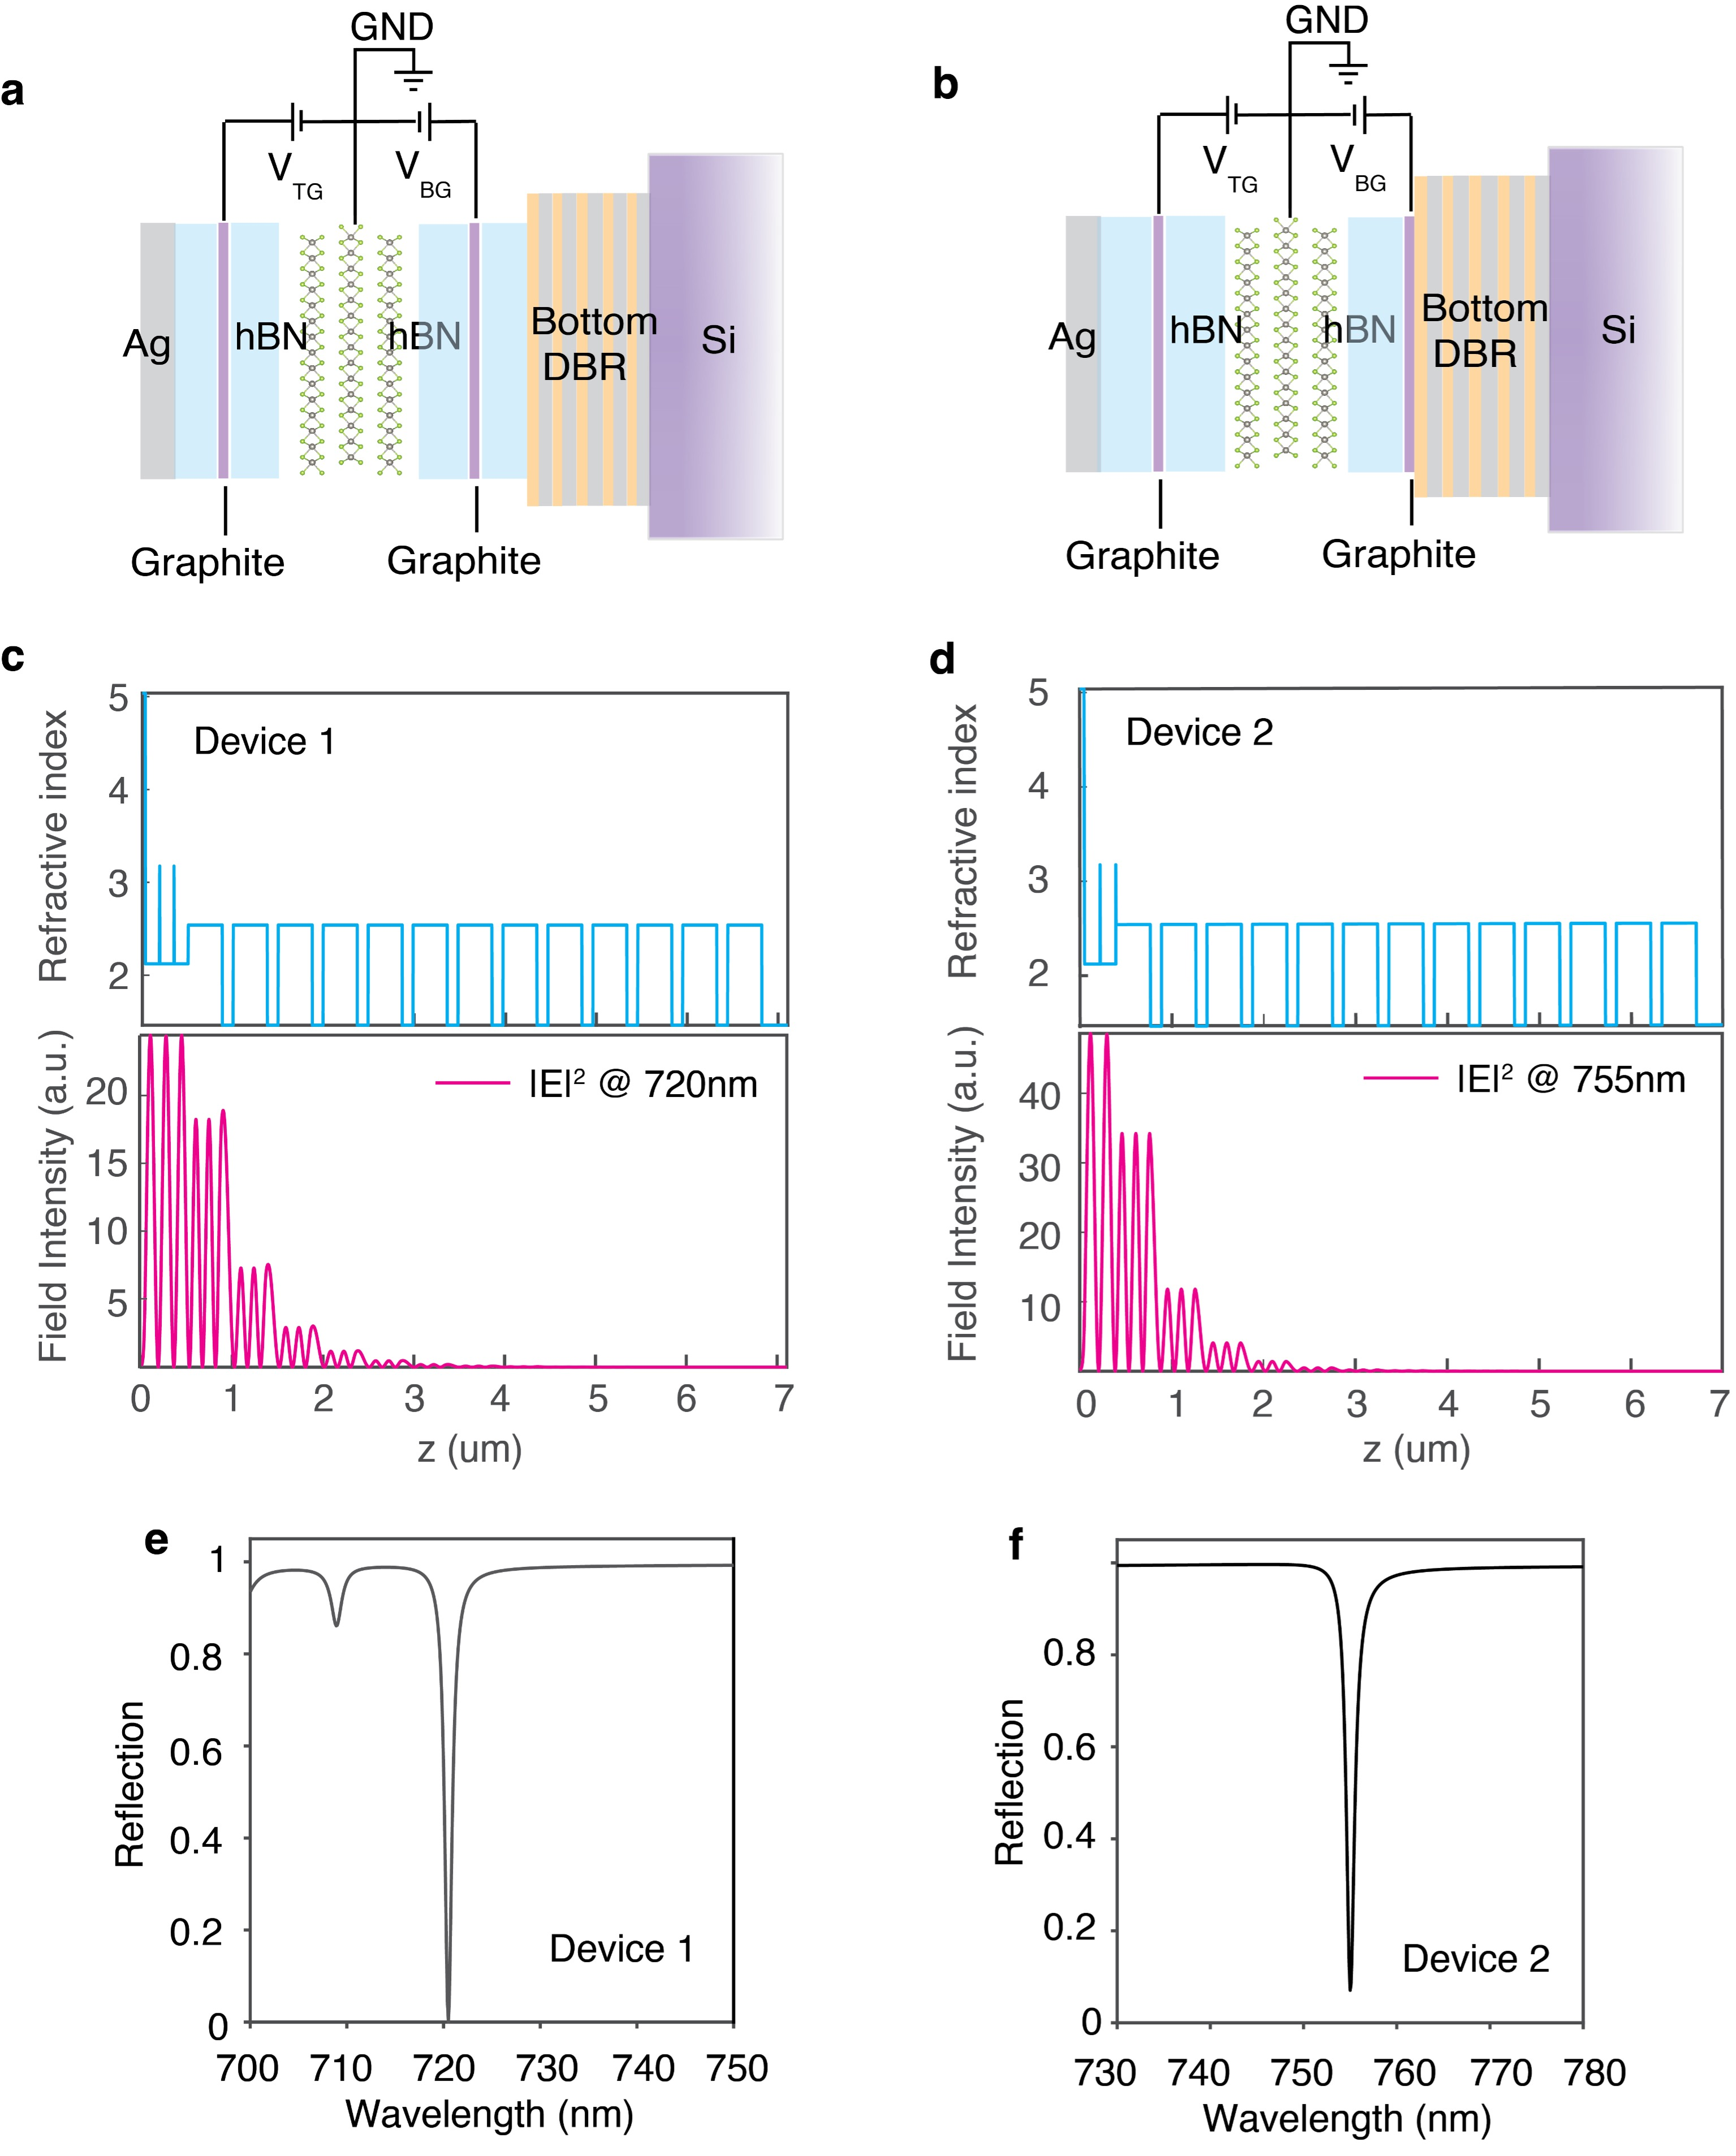
\includegraphics[width=0.8\textwidth]{Figures/C6/Fig6.7.jpg} % 
\end{center}
\caption[TMM Simulation of the Ag/DBR microcavity resonance for D1 and D2.] 
{\textbf{TMM Simulation of the Ag/DBR microcavity resonance for D1 and D2.}
\textbf{a, b,} Schematic of D1 and D2. \textbf{c, d,} Corresponded cavity structure and field intensity distribution $|E|^2$. In D1 there are in total three modes within the cavity, while in D2 there are two. 
However, the thinner cavity length structure should simplifier fabrication process, thus may lead to higher quality. \textbf{e, f,} Simulated cavity resonance. The linewidth is $\sim$ 0.7 nm for both resonances. 
}
\label{fig.6.7}
\end{figure}
\end{quote}
\renewcommand{\baselinestretch}{2}
\small\normalsize
% %/////////////////////// 

\section{Results and Discussions}
The cavity resonance of the first device D1 is designed for on resonantly couple to the exciton X$_A$ of the monolayer WSe$_2$ and slightly blue-detuned to the polaron in trilayer WSe$_2$. 
The cavity resonance of the second device D2 is designed red detuned to the trilayer WSe$_2$ polaron ($\Delta = -2 \hbar \Omega$). 
We first characterize the resonant energy and quality factor of the bare cavity, prior to the introduction of the monolayer or trilayer WSe$_2$. 
Due to the inherent inhomogeneity in the 2D stack, the linewidth of the cavity mode can be as narrow as 4 nm, corresponding to a quality factor of approximately 182.5.

\subsection{k-space imaging of the polariton dispersion in monolayer/ trilayer WSe$_2$}
To investigate exciton--polariton formation, we performed angle-resolved reflection imaging on both monolayer and trilayer WSe$_2$ embedded in the optical cavity in D1. 
Clear signatures of strong coupling between excitons and cavity photons were observed in both regions (see Figure~\ref{fig.6.8}). 
By fitting the upper and lower polariton with a coupled oscillator model, we extract the coupling strength $\hbar \Omega$ (half of the Rabi splitting) based on the Eq.~\ref{eq:LP_UP}.

% %/////////////////////// 
%Fig.6.7--------------
% \vspace{1em}
\renewcommand{\baselinestretch}{1}
\small\normalsize
\begin{quote}
\begin{figure}[htbp]
\begin{center}
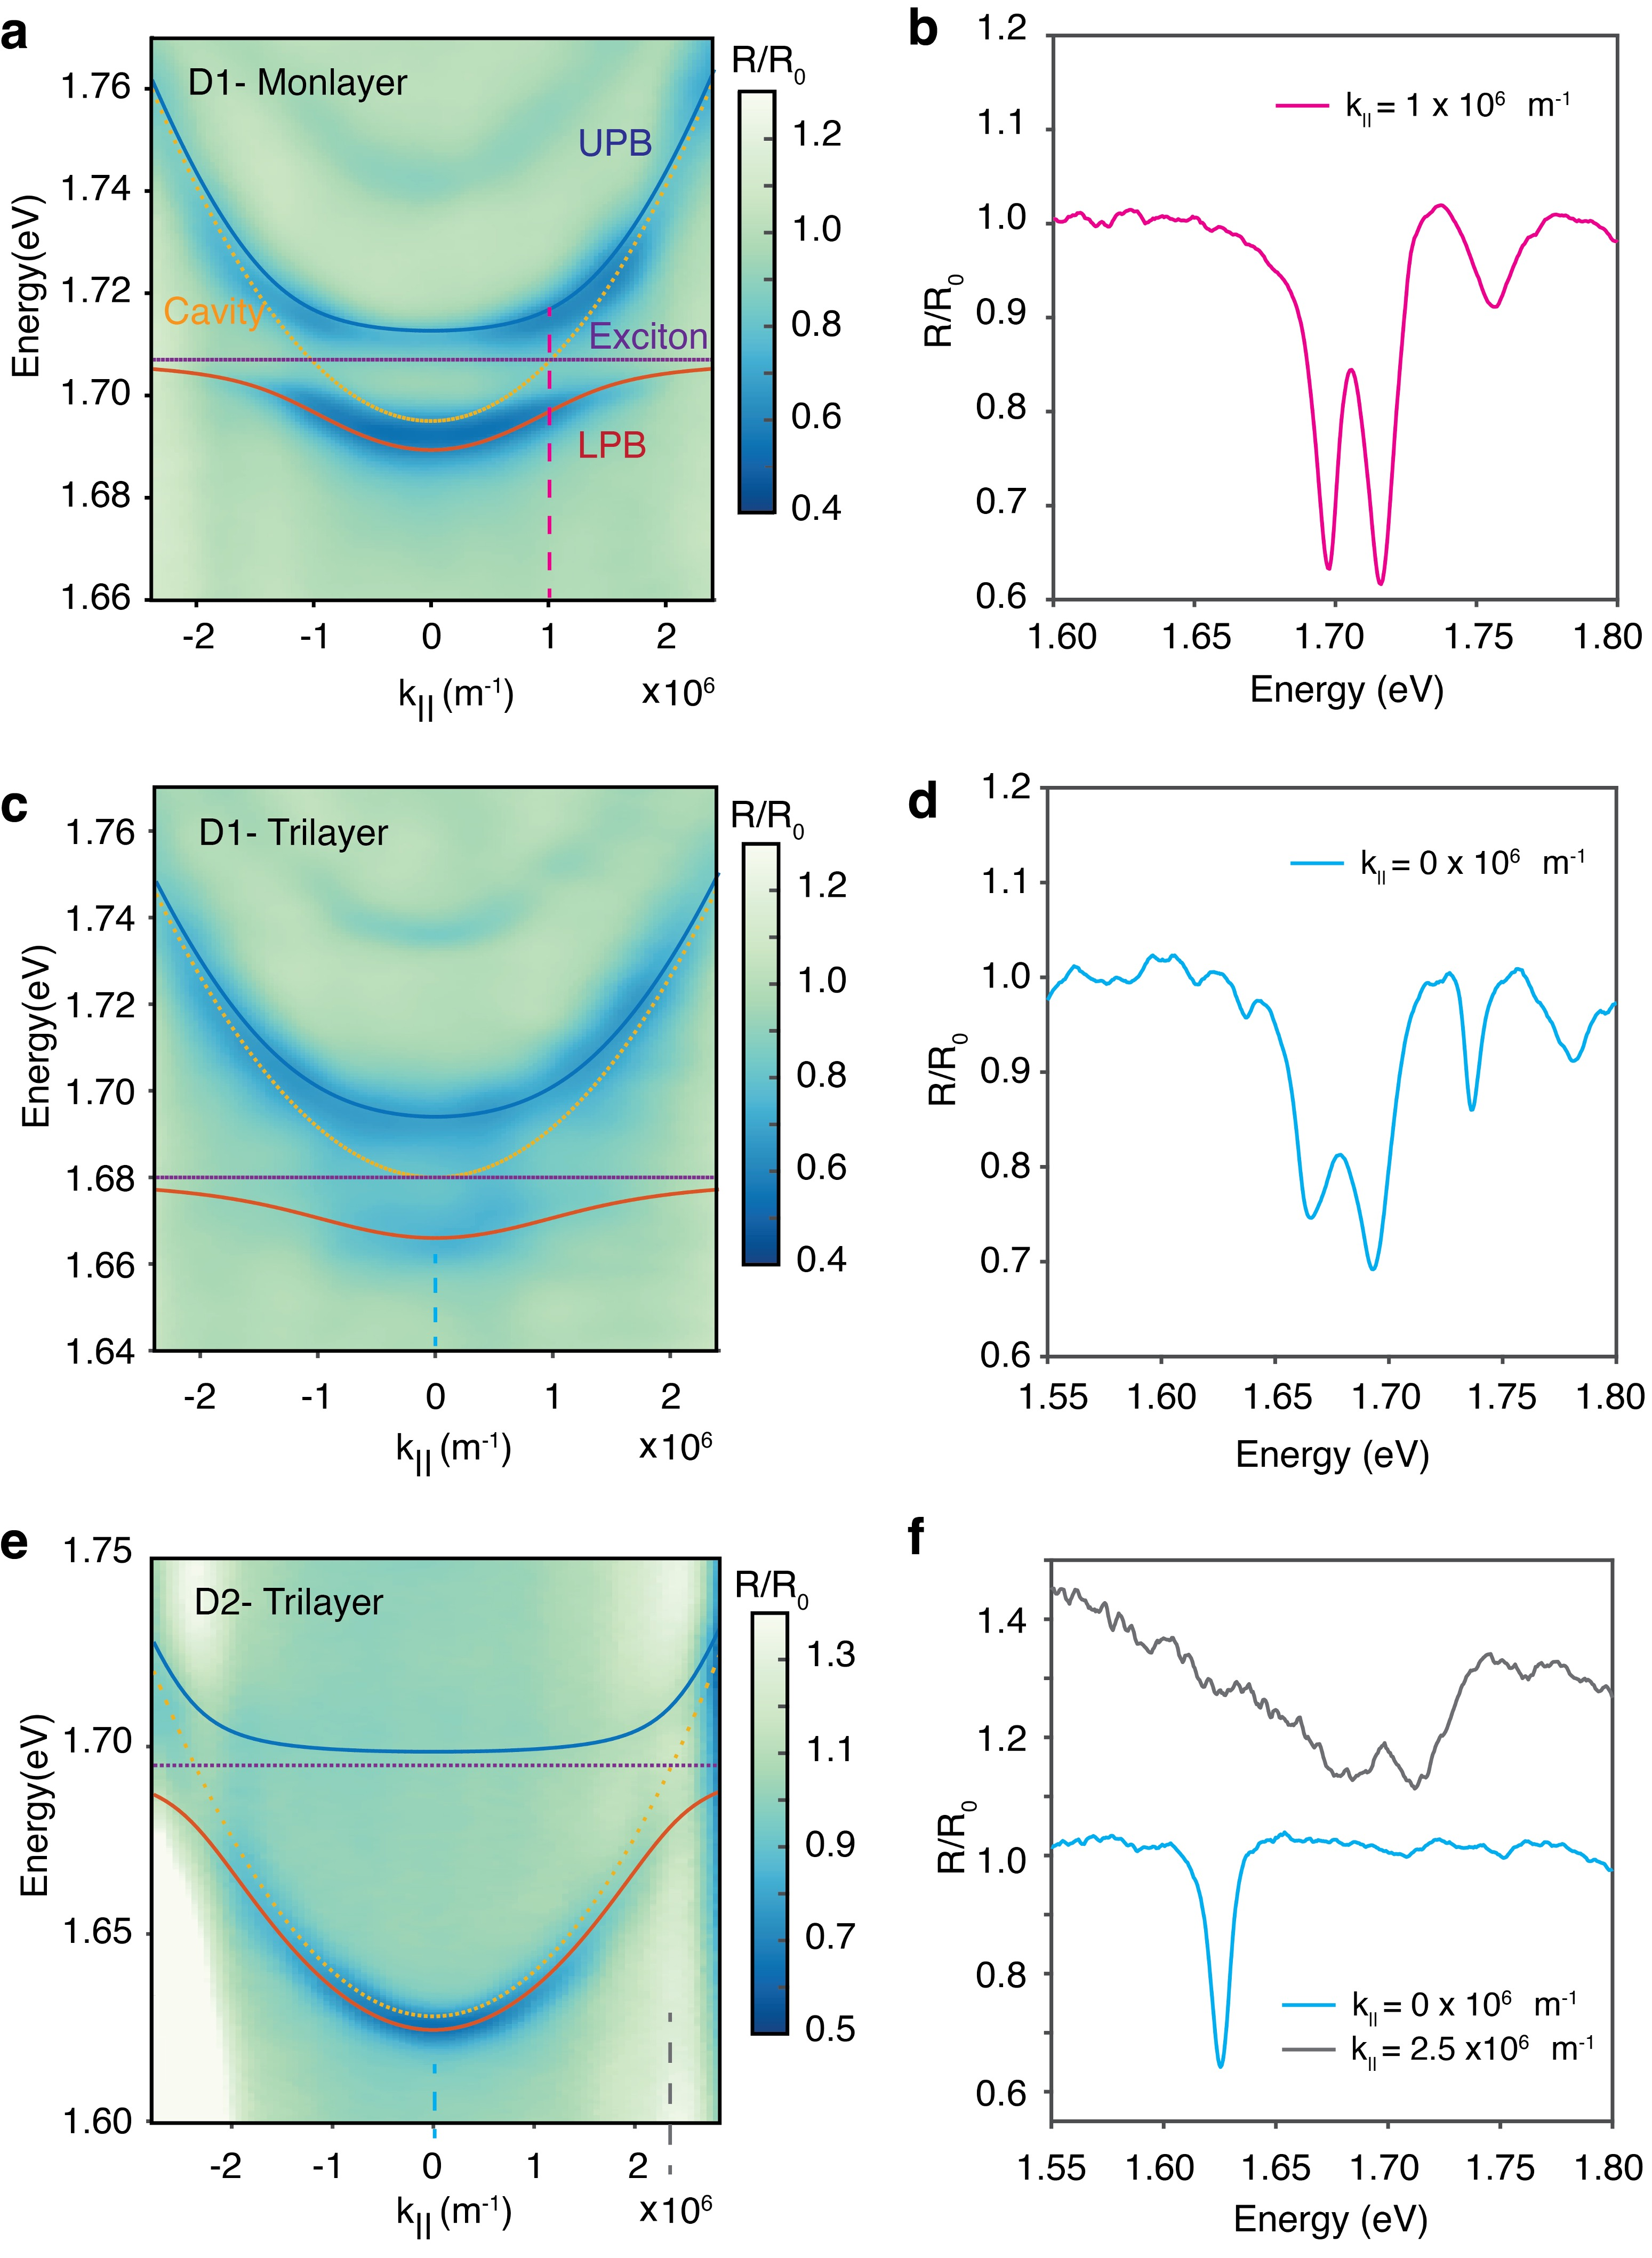
\includegraphics[width=0.8\textwidth]{Figures/C6/Fig6.8.jpg} % 
\end{center}
\caption[Strong coupling of exciton/polaron-polaritons in monolayer and trilayer WSe$_2$.] 
{\textbf{Strong coupling of exciton/polaron-polaritons in monolayer and trilayer WSe$_2$.}
\textbf{a}, Angle-resolved reflectance spectrum of exciton polaritons in D1 monolayer WSe$_2$ ($\Delta>0$).  
\textbf{c}, D1 trilayer WSe$_2$ ($\Delta=0$).  
\textbf{e}, D2 trilayer WSe$_2$ ($\Delta<0$).  
The blue and red solid lines show the fitted upper and lower polariton modes. 
The yellow dotted line corresponds to the cavity mode dispersion, and the purple dotted line marks the exciton energy.  
\textbf{b}, Reflectance spectrum of D1 monolayer at the anti-crossing position indicated by the magenta dashed line in (a).  
The energy splitting between LPB and UPB is $2\hbar\Omega \approx 20 \pm 1$~meV.  
\textbf{d}, Reflectance spectrum of D1 trilayer at $k_{\parallel}=0$ (where $E_{\mathrm{exc}} = E_{\mathrm{ph}}$), indicated by the blue dashed line in (c).  
The energy splitting between LPB and UPB is $2\hbar\Omega \approx 30 \pm 2$~meV.  
\textbf{f}, Reflectance spectrum of D2 trilayer at $k_{\parallel}=0$ (blue solid line) and at the anti-crossing region where $E_{\mathrm{exc}} = E_{\mathrm{ph}}$ (gray solid line).  
The energy splitting between LPB and UPB is $2\hbar\Omega \approx 33 \pm 3$~meV.
}
\label{fig.6.8}
\end{figure}
\end{quote}
\renewcommand{\baselinestretch}{2}
\small\normalsize
% %/////////////////////// 

For the monolayer, we obtained a coupling strength of about 10~meV for $\hbar\Omega$, while in the trilayer the value increases to $\sim$15~meV.
Given the cavity linewidth $\gamma_{\mathrm{cav}}$ (6--10~meV) and the polaron linewidth $\gamma_{\mathrm{polaron}}$ ($\sim$10~meV), these values satisfy the strong-coupling condition, $2\hbar\Omega > \gamma_{\mathrm{cav}} + \gamma_{\mathrm{polaron}}$.
Meeting this criterion confirms that the system supports polaritons as the new eigenmodes, as evidenced experimentally by the anti-crossing in the dispersion.
By contrast, in the weak-coupling regime the anti-crossing would be absent, and the exciton and photon resonances would remain uncoupled.

The stronger coupling observed in the trilayer can be attributed to the collective nature of light–matter interaction.
In multilayer structures, the vacuum Rabi splitting scales with the total oscillator strength coupled to the mode, which increases with the number of active layers $N$ if assuming uniform field overlap.
A standard approximation in multiple–quantum-well microcavities gives:
\begin{equation}
\hbar\Omega \sim \sqrt{\frac{N f}{L_{\mathrm{eff}}}}
\label{eq:Rabi_layers}
\end{equation}
where $f$ is the per-layer oscillator strength of the active transition and $L_{\mathrm{eff}}$ is the optical length of the cavity~\cite{ref41}.
This takes the same form as Eq.~\eqref{eq:rabi}.
This therefore predicts a square-root dependence of $\hbar\Omega$ on the number of embedded layers, so a trilayer ($N=3$) naturally exhibits a larger splitting than a monolayer ($N=1$).

This square-root scaling is well established in strongly coupled systems such as GaAs and CdTe multiple–quantum-well microcavities, where collective enhancement from multiple wells boosts the light–matter interaction.
The same principle applies to TMDs: the trilayer exhibits enhanced coupling because the effective oscillator strength is multiplied by the number of coupled layers.

Furthermore, in the trilayer region the exciton resonance (1.69~eV) lies close to the cavity photon energy, which causes the upper polariton branch to remain near the bare cavity dispersion while the lower polariton branch follows the excitonic dispersion, consistent with the measured anti-crossing.

\subsection{Electrically tunable exciton/polaron-polaritons in monolayer and trilayer WSe$_2$}
Electrical control of van der Waals heterostructures enables dynamic tuning of many-body interactions in TMD layers, giving rise to the formation of exciton–polarons.
Because polaritons inherit the intrinsic properties of their excitonic component, electrical gating serves as an effective knob to modulate their dispersion, composition, and nonlinear response.
Such tunability offers a pathway toward reconfigurable polaritonic devices, where propagation, confinement, and interaction strength can be actively controlled without altering the cavity structure.

To investigate these effects, we measured gate-dependent reflectance to access the polaron – polariton states.
For more efficient and uniform doping, a halogen lamp was used to illuminate a large area of the sample, thereby enhancing charge transfer at the locally probed spot during gating.
In the monolayer region, as shown in Figure~\ref{fig.6.9}a, the two polariton branches exhibit smooth energy blueshifts under intrinsic and low-doping conditions.
This behavior arises from phase-space filling of the repulsive polaron in monolayer WSe$_2$ under doping.
At higher hole-doping levels, attractive polaron–polaritons emerge, but with a reduced energy splitting ($\sim$13~meV) compared to the intrinsic case ($\sim$22~meV).

% %/////////////////////// 
%Fig.6.9--------------
% \vspace{1em}
\renewcommand{\baselinestretch}{1}
\small\normalsize
\begin{quote}
\begin{figure}[htbp]
\begin{center}
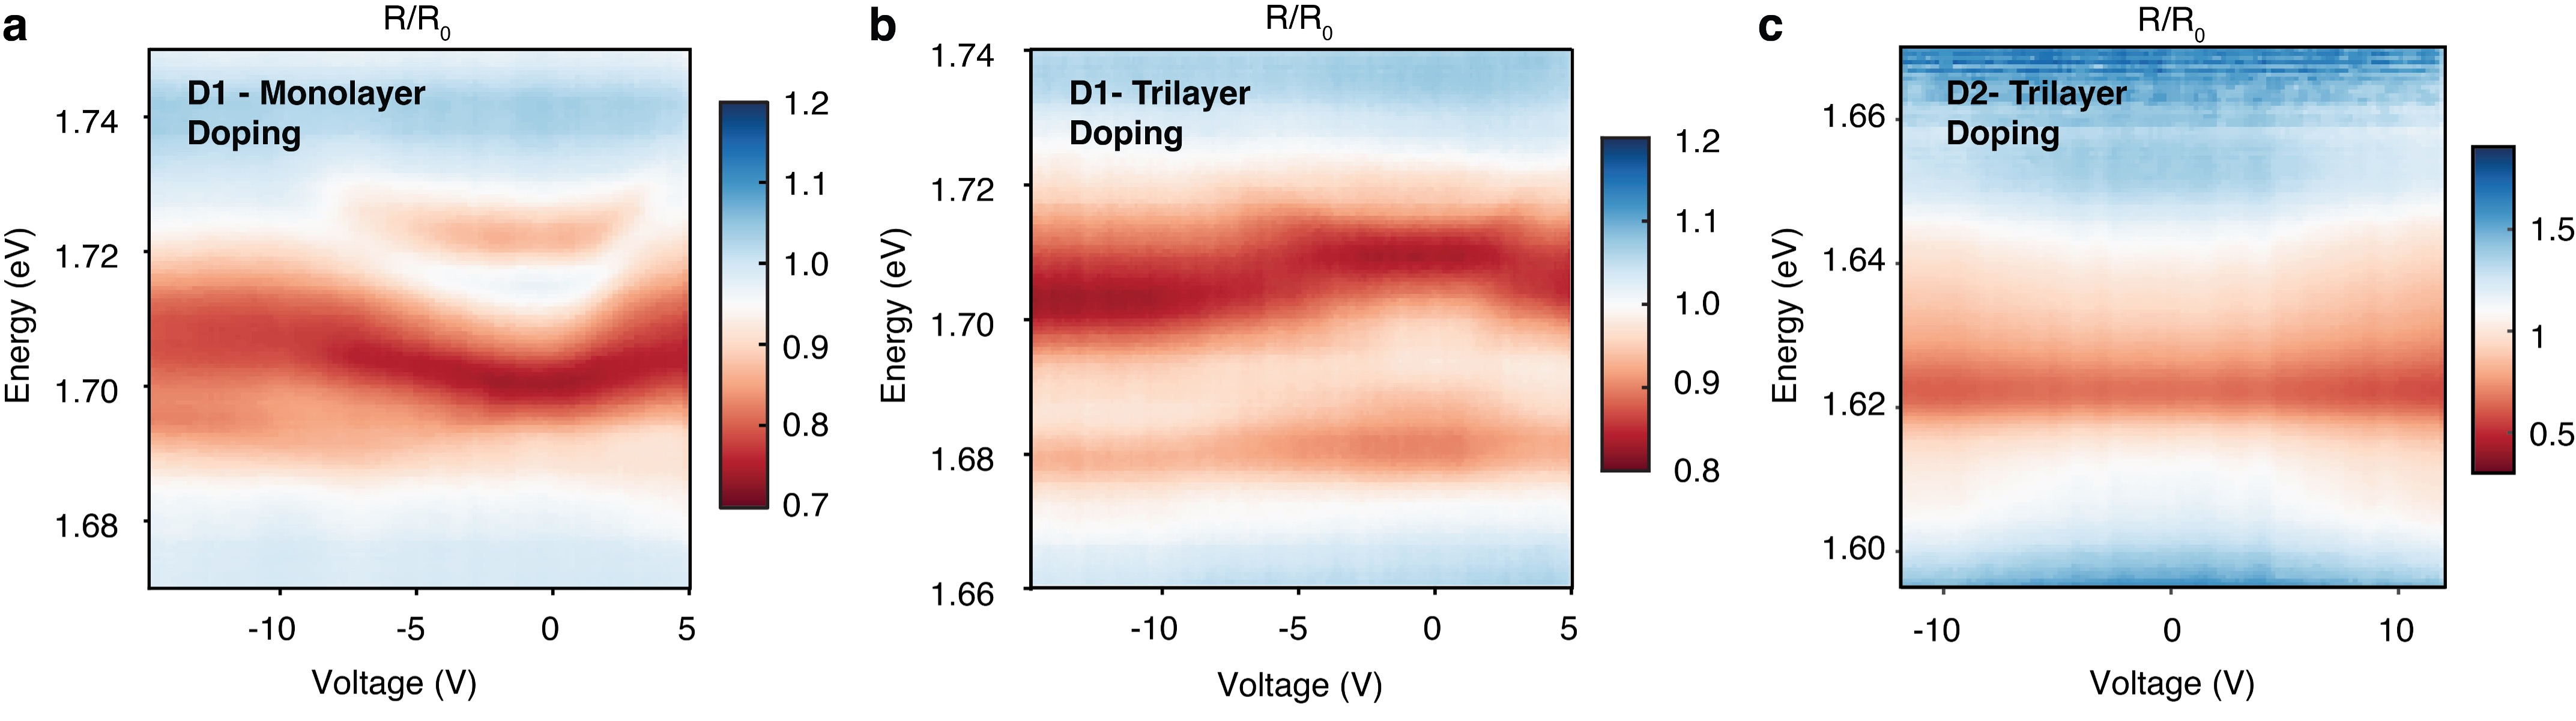
\includegraphics[width=1\textwidth]{Figures/C6/Fig6.9.jpg} % 
\end{center}
\caption[Doping dependent map of reflectance at 5 K.] 
{\textbf{Doping dependent map of reflectance at 5 K.}
Normalized reflectance as a function of gate voltage in \textbf{a,} monolayer and \textbf{b,} trilayer WSe$_2$ in D1, \textbf{c,} trilayer WSe$_2$ in D2.
} 
\label{fig.6.9}
\end{figure}
\end{quote}
\renewcommand{\baselinestretch}{2}
\small\normalsize
% %/////////////////////// 
In contrast, in the trilayer WSe$_2$ region of D1, we observe consistently large Rabi splittings across all gating regimes, with an exciton–polariton splitting of $\sim$ 30.5~meV and a polaron–polariton splitting of $\sim$ 28.3~meV.  
The persistence of large energy splittings under all electrical gating conditions in the trilayer region is expected, since polarons in trilayers possess larger oscillator strength and therefore couple more strongly to the cavity photon.  

By comparison, in the D2 trilayer WSe$_2$ region with detuning $\Delta \sim -2\hbar\Omega$, the lower polariton branch has a high photon fraction and is therefore expected to show minimal gate dependence.  
Experimentally, we indeed observe only a broadening of the dip feature with increasing gate voltage, which can be attributed to linewidth broadening of the polaron species arising from exciton–carrier scattering.

\subsection{Distinct polariton nonlinear behavior with power}
Next, we studied the polariton nonlinear behavior in the monolayer and trilayer regions in D1. 
A supercontinuum white laser was used for broadband power dependent reflection measurements, with the wavelength range selected by an acousto-optic tunable filter (AOTF): 715–755 nm for the trilayer region and 715–750 nm for the monolayer region (see in Figure~\ref{fig.6.10}).

% %/////////////////////// 
%Fig.6.10--------------
% \vspace{1em}
\renewcommand{\baselinestretch}{1}
\small\normalsize
\begin{quote}
\begin{figure}[htbp]
\begin{center}
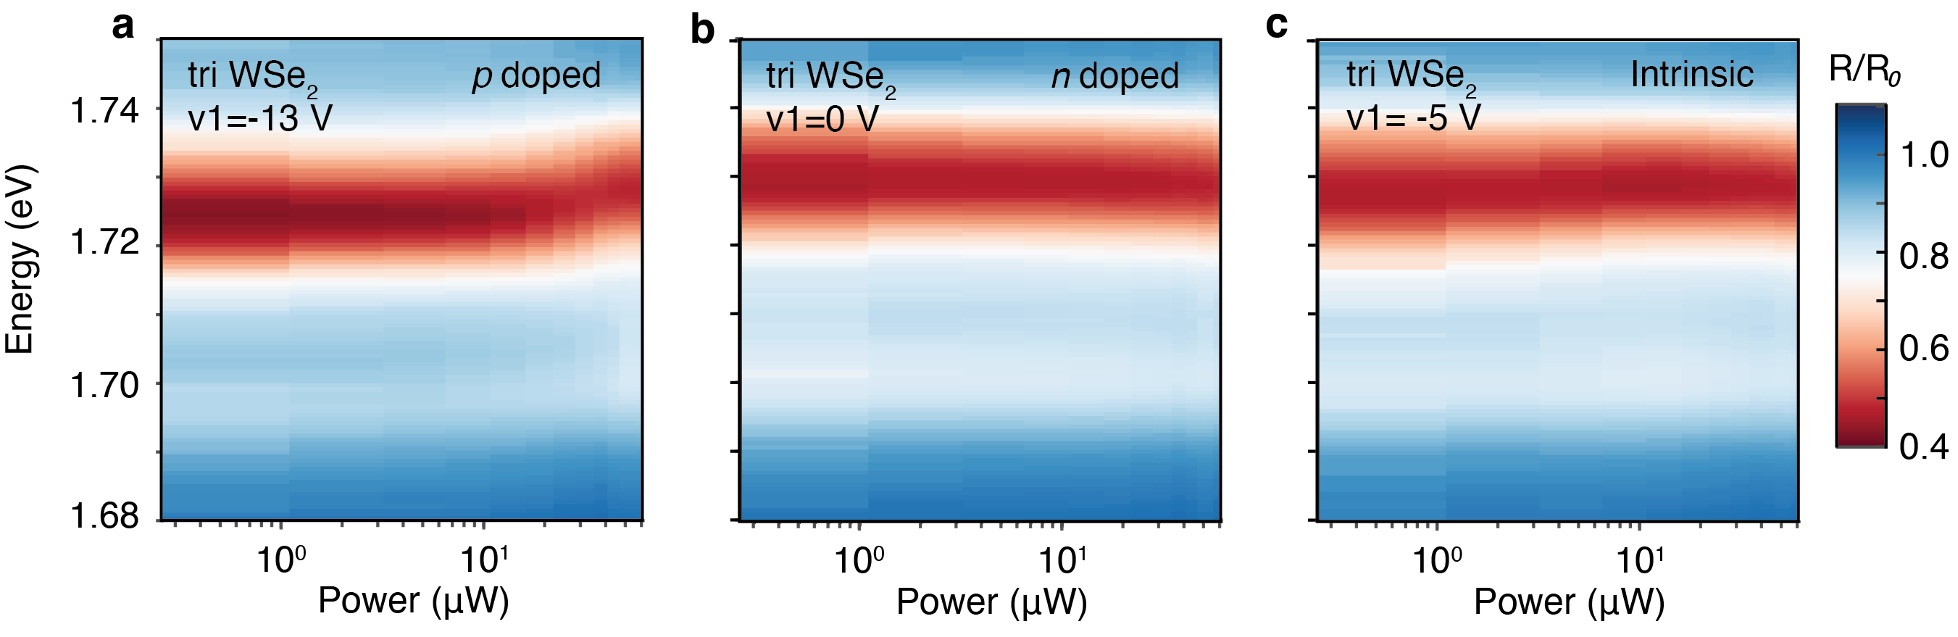
\includegraphics[width=1\textwidth]{Figures/C6/Fig6.10.jpg} % 
\end{center}
\caption[Power dependent reflectance of polaritons in trilayer WSe$_2$.] 
{\textbf{Power dependent reflectance of polaritons in trilayer WSe$_2$.}
\textbf{a,} LP and UP polaron polariton energy blueshift as a function of the pulsed laser excitation average power (715-755 nm). Both the polariton species shows an energy blueshift with power, while for the \textbf{b,} electron dope and \textbf{c,} intrinsic case this nonlinear behavior is absent.
} 
\label{fig.6.10}
\end{figure}
\end{quote}
\renewcommand{\baselinestretch}{2}
\small\normalsize
% %/////////////////////// 
In the trilayer region, we compared two doping conditions at: intrinsic (V1 = -5 V) and hole doped side (V1 = -13V). 
This nonzero voltage corresponded intrinsic case is due to the inefficient doping across the sample by using the supercontinuum laser as a small excitation spot. 
Under hole doping, both polariton branches exhibited energy blueshifts with increasing excitation power: the lower polariton shifted by ~4.3 meV, while the upper branch shifted by ~3.8 meV.
The difference in blueshift can be attributed to the unequal exciton fractions in the LPB and UPB, since the nonlinear interaction between the polaritons contributed from the excitonic part scales as $\lvert X_{(k_{\parallel})} \rvert^{4} \cdot g_{\mathrm{exc}}$. 
In contrast, under intrinsic doping, only the upper branch showed an energy redshift of about 1.2 meV, while the lower branch exhibited no significant change.

In the monolayer region, within the same power range, no energy shift was observed. 
However, when we further increased both the excitation power and the laser bandwidth, the lower and upper polariton energies shifted toward each other. 
This behavior is consistent with phase space filling induced polariton nonlinearity: at high non-resonant excitation power, 
the exciton density increases, and phase-space filling reduces the available oscillator strength, weakening the light–matter coupling and thereby decreasing the Rabi splitting.

We then quantitatively analyzed the photon flux required to induce the observed polariton shift and compared it with the polaron nonlinearity. 
For an excitation bandwidth of 715--755~nm, a lower polariton blueshift of 4.3~meV corresponded to approximately $2.5 \times 10^{5}$ photons per~$\mu$m$^{2}$. 
In homotrilayer WSe$_2$, a comparable nonlinear shift ($\sim$4~meV) was observed at a similar photon flux. 
However, due to the large cavity leakage (cavity mode FWHM $\sim$10~nm), the polariton linewidth ($\sim$16~meV) is significantly broader than the polaron linewidth ($\sim$10~meV). 
In this case, the polariton linewidth is primarily limited by the cavity quality.

\section{Summary and Outlook}
In summary, we fabricated electrically tunable one-dimensional microcavity with trilayer WSe$_2$ van der Waals heterostructures embedded. 
By varying the thickness of the encapsulating hBN layers, we achieved different detuning $\Delta$ conditions at zero in-plane wavevector. 
At $T = 5$~K, we observed strong coupling between excitons/polarons and cavity photons, as evidenced by the formation of lower and upper polaritons. 
Angle-resolved reflectivity measurements revealed clear anti-crossing behavior between the polariton branches. 
The extracted Rabi splitting of the exciton–polariton in the trilayer was approximately 30~meV, significantly larger than the 20~meV splitting observed in the monolayer, which is due to the enhanced oscillator strength of excitons/polarons in the trilayer. 
Notably, strong coupling persists across a wide range of gate voltages in trilayers, in contrast to the monolayer case, where it disappears under similar conditions.  

Under resonant excitation of the polariton modes in trilayer WSe$_2$, we observed clear nonlinear responses in the weak-pump regime. 
In the hole-doped case, both the lower and upper polariton branches exhibited energy blueshifts with increasing pump power, whereas no such shifts were detected under intrinsic or electron-doped conditions. 
This behavior is consistent with polaron-mediated interactions in homotrilayer WSe$_2$, indicating that excitonic interactions dominate the polariton nonlinearity at low excitation densities. 
At higher pump powers, the Rabi splitting progressively decreased, which we attribute to phase-space filling effects that reduce the available excitonic oscillator strength and weaken the light–matter coupling.  

Overall, our results demonstrate that polaron–polaritons in trilayer WSe$_2$ combine strong oscillator strength with pronounced optical nonlinearities under hole doping. 
These properties establish trilayer WSe$_2$ microcavities as a promising platform for exploring bright, strongly interacting polariton systems, and for advancing towards the quantum nonlinear regime, where phenomena such as polariton blockade and strongly correlated photonic states are anticipated.

%Chapter 7

\renewcommand{\thechapter}{7}

\chapter{Summary and Outlook}
\label{chap7}
section{Summary}

section{Outlook}

\titleformat{\chapter}

% {\normalfont\large}{Appendix \thechapter:}{1em}{}

%Appendix
\appendix
\renewcommand{\thechapter}{A}
\renewcommand{\chaptername}{Appendix A}

\chapter{Clean room process}

\label{chapA}

\renewcommand{\baselinestretch}{1}
\small\normalsize

% \addcontentsline{toc}{chapter}{Bibliography}
% \include{Bibliography} %To be used when typing your own bibliography
% \bibliographystyle{unsrt}


%When using Bibtex, delete the previous line and use the following
%three lines:
\newpage
\chapter*{Bibliography}
\addcontentsline{toc}{chapter}{Bibliography}

% suppress the automatic heading inside thebibliography
\begingroup
  \renewcommand{\bibname}{}% keep it empty so no extra title is printed
  \bibliographystyle{unsrt}
  \bibliography{paper2}
\endgroup

% \bibliographystyle{unsrt}
% \bibliography{paperpile} %replace "Galactic,Dottie" with the
%                 file name(s) of your bib file(s)

%When using Natbib, use the following three lines:
%\newpage
%\bibliographystyle{unsrtnat}
%\bibliography{Galactic,Dottie} %replace "Galactic,Dottie" with the
%                 file name(s) of your bib file(s)

\end{document}
